\documentclass[a4paper,12pt]{article}
\usepackage[T1]{fontenc}
\usepackage[utf8]{inputenc}
\usepackage[polish]{babel}
\usepackage{graphicx}
\usepackage{geometry}
\usepackage{enumitem}
\usepackage{hyperref}
\usepackage{xcolor}
\usepackage{float}
\usepackage{array}    % Dla zaawansowanych opcji kolumn tabeli
\usepackage{tabularx} % Do tworzenia tabel o zadanej szerokości z kolumnami typu X
% \usepackage{enumitem} % Jeśli chcesz mieć większą kontrolę nad formatowaniem list (np. mniejsze odstępy) - na razie usunąłem specyficzne opcje tego pakietu
\usepackage{longtable}
\usepackage{array} % Często przydatny z longtable dla zaawansowanych opcji kolumn


\geometry{margin=2.5cm}

\title{\textbf{OpenTravel}\\\
\large{Propozycja kompleksowej platformy do planowania i realizacji podróży}}
\author{Mateusz Bielówka, Maksim Dziatkou, Patryk Chamera
\\ Berenike Banek, Karol Bystrek}
\date{\today}

\begin{document}
\maketitle

\begin{figure}[H]
    \centering
    
\includegraphics[width=\linewidth]{images/logo.png}
    \label{fig:logo}
\end{figure}

\newpage

\tableofcontents
\newpage

\section*{Wprowadzenie i cel projektu}
Celem projektu OpenTravel jest stworzenie innowacyjnej aplikacji mobilnej, która zintegruje funkcjonalności najpopularniejszych aplikacji transportowych w jednym, intuicyjnym interfejsie.
Projekt zakłada połączenie możliwości narzędzi takich jak Jakdojade czy Uber, a także aplikacji służących do zakupu biletów kolejowych i wyszukiwania lotów.
Głównym założeniem jest opracowanie kompleksowej platformy, która ma na celu zaspokojenie wszystkich potrzeb transportowych użytkowników bez konieczności przełączania się między różnymi aplikacjami.
OpenTravel ma umożliwić płynne planowanie podróży praktycznie każdym środkiem transportu, co stanowi odpowiedź na rosnące zapotrzebowanie na zintegrowane rozwiązania w dziedzinie mobilności.

\section{Ogólny opis systemu i kluczowe funkcjonalności}
Platforma OpenTravel projektowana jest z myślą o dostarczeniu użytkownikom wszechstronnego narzędzia do zarządzania podróżami. Poniżej przedstawiono kluczowe obszary funkcjonalne, które system ma obejmować.

\subsection*{Transport publiczny}
W ramach funkcjonalności związanych z transportem publicznym, aplikacja OpenTravel ma oferować możliwość zakupu biletów jednorazowych i okresowych na komunikację miejską, potencjalnie eliminując potrzebę posiadania gotówki czy dedykowanej karty miejskiej.
Planuje się, że użytkownicy będą mieli dostęp do aktualnych rozkładów jazdy wszystkich środków transportu publicznego, w miarę możliwości w czasie rzeczywistym, oraz będą mogli otrzymywać powiadomienia o ewentualnych opóźnieniach lub zmianach w kursowaniu.
System ma umożliwiać planowanie optymalnych tras z uwzględnieniem przesiadek oraz zapisywanie najczęściej używanych połączeń dla szybkiego dostępu.

\subsection*{Przejazdy taksówkami}
Aplikacja ma umożliwiać zamawianie przejazdów taksówkami z precyzyjnym określeniem miejsca odbioru i punktu docelowego.
Przewiduje się, że przed złożeniem zamówienia użytkownik otrzyma kalkulację przewidywanego kosztu przejazdu oraz będzie miał możliwość wyboru klasy pojazdu (np. standard, premium, pojazd dostosowany do przewozu osób z niepełnosprawnościami).
W trakcie oczekiwania na taksówkę, użytkownik powinien móc śledzić lokalizację zamówionego pojazdu w czasie rzeczywistym.
System ma również oferować funkcję oceniania kierowców po zakończonym przejeździe oraz realizację bezgotówkowych rozliczeń bezpośrednio przez aplikację.

\subsection*{Bilety kolejowe}
W zakresie transportu kolejowego, OpenTravel ma umożliwiać wyszukiwanie dostępnych połączeń krajowych i międzynarodowych oraz zakup biletów na pociągi różnych przewoźników obsługujących dany region.
Planuje się, że użytkownicy będą mogli korzystać z interaktywnego wyboru miejsca w pociągu z wizualizacją układu wagonu, jeśli API przewoźnika na to pozwoli.
Zakupione bilety mają być przechowywane w formie elektronicznej, gotowe do kontroli.
Aplikacja ma również za zadanie dostarczać powiadomienia o opóźnieniach, odwołaniach lub zmianach peronów, a także potencjalnie integrować się z programami lojalnościowymi przewoźników kolejowych.

\subsection*{Loty}
Moduł lotniczy ma oferować zaawansowane wyszukiwanie połączeń z możliwością filtrowania według ceny, czasu trwania czy liczby przesiadek.
Użytkownicy powinni móc porównywać ceny lotów z różnych linii lotniczych i platform sprzedażowych oraz otrzymywać alerty o specjalnych ofertach i promocjach na wybrane kierunki.
Aplikacja ma dążyć do umożliwienia odprawy online bezpośrednio z jej poziomu, dostarczania informacji o mapach lotnisk, bramkach, opóźnieniach i udogodnieniach, a także pozwolić na rezerwację transportu z i na lotnisko.

\newpage
\section{Analiza wymagań funkcjonalnych}
Niniejszy rozdział poświęcony jest szczegółowej analizie wymagań funkcjonalnych systemu OpenTravel. Celem tej analizy jest precyzyjne zdefiniowanie, jakie działania system będzie realizował oraz jakie funkcje udostępni swoim użytkownikom i systemom zewnętrznym. Zakres analizy obejmuje identyfikację wszystkich kluczowych interakcji użytkownika z systemem oraz interakcji między komponentami systemu a stowarzyszonymi usługami.

\subsection{Aktorzy Systemu OpenTravel}
W ramach systemu OpenTravel zidentyfikowano kluczowe role, zwane aktorami, które będą wchodzić w interakcję z platformą. Aktorzy reprezentują zarówno użytkowników końcowych, jak i zewnętrzne systemy lub podmioty współpracujące. Poniżej przedstawiono ich listę wraz z krótkim opisem.

\begin{description}
    \item[\textbf{Użytkownik}] Główny aktor systemu, reprezentujący osobę fizyczną korzystającą z aplikacji do planowania podróży, wyszukiwania połączeń, zakupu biletów oraz zarządzania rezerwacjami. Obejmuje zróżnicowane profile, takie jak podróżny indywidualny, turysta, student, senior czy pracownik korporacyjny.
    \item[\textbf{Użytkownik z niepełnosprawnością}] Podtyp \textit{Użytkownika}, który dodatkowo korzysta ze specyficznych funkcji systemu ułatwiających podróżowanie, np. filtrowania pod kątem dostępności infrastruktury lub rezerwacji usług transportowych dostosowanych do jego potrzeb.
    \item[\textbf{Kierowca}] Aktor wykonujący usługi przewozowe; interakcja z systemem OpenTravel obejmuje przyjmowanie zleceń, zarządzanie statusami kursów oraz rozliczenia za pośrednictwem platformy.
    \item[\textbf{Administrator systemu}] Osoba lub zespół odpowiedzialny za zarządzanie operacyjne i techniczne platformą OpenTravel, w tym konfigurację, monitorowanie, zarządzanie użytkownikami, treścią oraz integracjami z systemami zewnętrznymi.
    \item[\textbf{Przewoźnik Miejski}] Zewnętrzny podmiot (np. Zarząd Transportu Miejskiego, Miejskie Przedsiębiorstwo Komunikacyjne) lub jego system informatyczny, odpowiedzialny za dostarczanie do OpenTravel danych dotyczących transportu publicznego (rozkłady jazdy, trasy, taryfy biletowe, dane czasu rzeczywistego) oraz umożliwiający zakup i obsługę biletów na komunikację miejską poprzez integrację z platformą.
    \item[\textbf{Przewoźnik Prywatny (dla przejazdów typu taxi/na żądanie)}] Zewnętrzny podmiot świadczący usługi transportowe typu taxi lub inne przejazdy na żądanie. Aktor ten udostępnia dane o swoich trasach, taryfach i dostępności pojazdów, integrując je z platformą OpenTravel.
    \item[\textbf{Przewoźnik Kolejowy}] Zewnętrzny podmiot lub system dostarczający dane o połączeniach kolejowych (rozkłady, ceny, dostępność, status pociągów) i odbierający informacje o sprzedanych biletach/rezerwacjach za pośrednictwem OpenTravel.
    \item[\textbf{Przewoźnik Lotniczy}] Zewnętrzny podmiot lub system (linia lotnicza, system rezerwacyjny, agregator) udostępniający dane o lotach (rozkłady, ceny, dostępność, status) i umożliwiający procesy rezerwacji, zakupu oraz potencjalnie odprawy online poprzez platformę OpenTravel.
    \item[\textbf{Dostawca Usług Płatności}] Zewnętrzny system (np. bramka płatnicza) integrowany z OpenTravel, odpowiedzialny za bezpieczne przetwarzanie i autoryzację transakcji finansowych dokonywanych przez Użytkowników.
\end{description}

\subsection{Lista Przypadków Użycia}
Poniższa lista przedstawia zidentyfikowane przypadki użycia dla systemu OpenTravel, pogrupowane według głównych obszarów funkcjonalnych. Każdy przypadek użycia reprezentuje konkretną interakcję aktora z systemem, mającą osiągnąć określony cel. Diagramy przypadków użycia wizualizują te interakcje oraz powiązania między aktorami a przypadkami użycia w poszczególnych modułach systemu.

\subsubsection{Zarządzanie Kontem i Funkcje Ogólne}
\begin{enumerate}[label=\arabic*.]
    \item Rejestracja w systemie (Nowy Użytkownik, Nowy Kierowca)
    \item Logowanie do systemu (Użytkownik, Administrator systemu, Kierowca)
    \item Zarządzanie danymi konta (Użytkownik, Administrator systemu, Kierowca)
    \item Odzyskiwanie hasła (Użytkownik, Administrator systemu, Kierowca)
    \item Zarządzanie metodami płatności (Użytkownik)
    \item Dodawanie zniżek do konta (Użytkownik)
    \item Zarządzanie danymi do faktury (Użytkownik)
    \item Przeglądanie historii podróży (Użytkownik)
    \item Przeglądanie historii kursów (Kierowca)
    \item Przeglądanie historii zakupionych biletów (Użytkownik)
    \item Konfiguracja preferencji powiadomień (Użytkownik)
    \item Wyświetlanie aktywnego biletu do kontroli (Użytkownik)
    \item Uzyskiwanie pomocy (Użytkownik, Kierowca)
    \item Zarządzanie kontami użytkowników (Administrator systemu)
    \item Monitorowanie stanu systemu i logów (Administrator systemu)
    \item Generowanie raportów systemowych (Administrator systemu)
    \item Wybór preferowanych środków transportu (Użytkownik)
    \item Definiowanie preferencji dostępności (Użytkownik z niepełnosprawnością, Użytkownik)
    \item Podgląd zarobków (Kierowca)
    \item Dodawanie biletów/rezerwacji do kalendarza (Użytkownik)
\end{enumerate}
\begin{figure}[H]
    \centering
    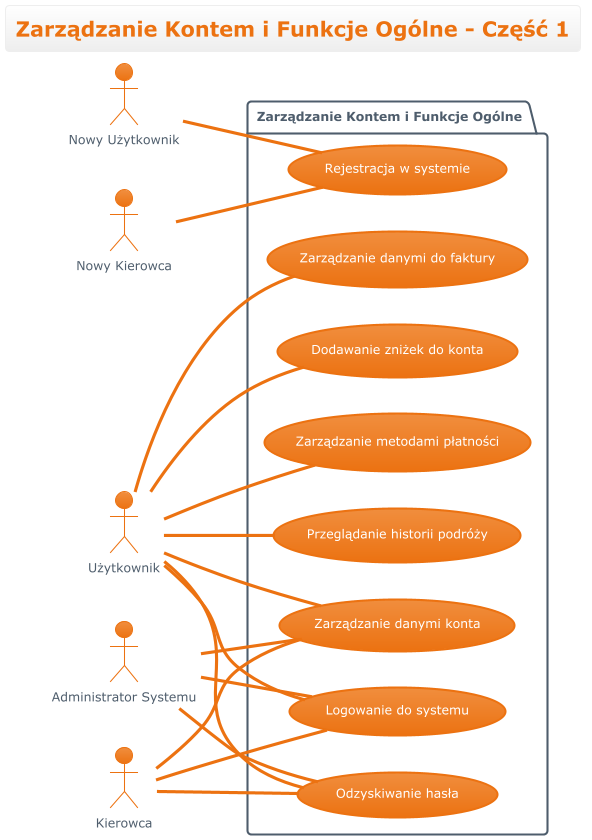
\includegraphics[width=0.8\linewidth]{diagramy/przypadki_uzycia/images/diagram_zarzadzanie_kontem_1.png}
    \caption{Diagram przypadków użycia: Funkcje ogólne - część 1}
    \label{fig:diag_zk_1}
\end{figure}
\begin{figure}[H]
    \centering
    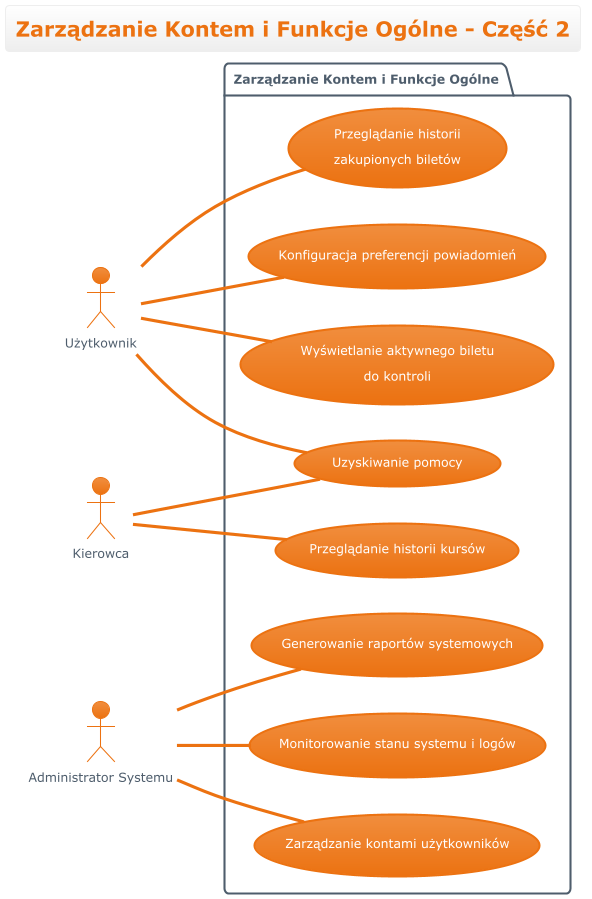
\includegraphics[width=0.8\linewidth]{diagramy/przypadki_uzycia/images/diagram_zarzadzanie_kontem_2.png}
    \caption{Diagram przypadków użycia: Funkcje ogólne - część 2}
    \label{fig:diag_zk_2}
\end{figure}
\begin{figure}[H]
    \centering
    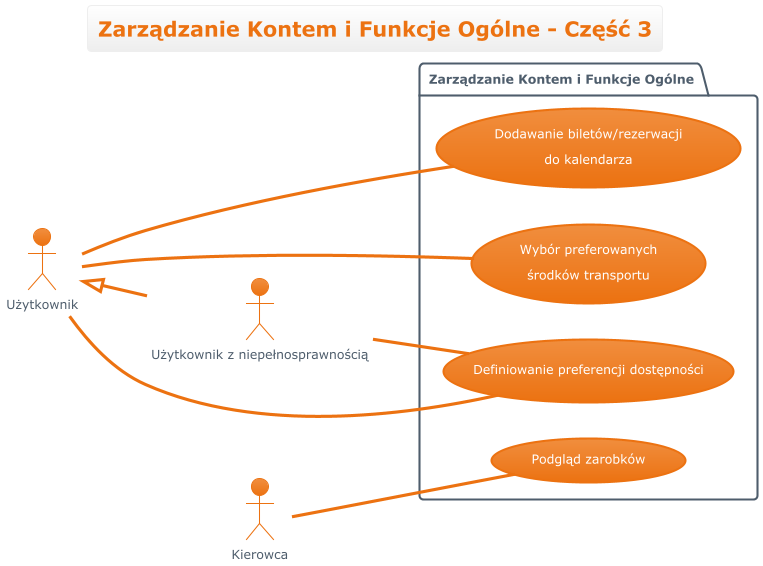
\includegraphics[width=0.8\linewidth]{diagramy/przypadki_uzycia/images/diagram_zarzadzanie_kontem_3.png}
    \caption{Diagram przypadków użycia: Funkcje ogólne - część 3}
    \label{fig:diag_zk_3}
\end{figure}

\subsubsection{Transport Publiczny}
\begin{enumerate}[label=\arabic*.]
    \item Wyszukiwanie połączeń komunikacji miejskiej (Użytkownik)
    \item Wyświetlanie rozkładu jazdy komunikacji miejskiej (Użytkownik)
    \item Zakup biletu jednorazowego na komunikację miejską (Użytkownik, Przewoźnik Miejski, Dostawca Usług Płatności)
    \item Zakup biletu okresowego na komunikację miejską (Użytkownik, Przewoźnik Miejski, Dostawca Usług Płatności)
    \item Planowanie trasy multimodalnej (Użytkownik)
    \item Zapisywanie ulubionych tras i przystanków (Użytkownik)
    \item Otrzymywanie powiadomień o zmianach w komunikacji miejskiej (Użytkownik)
    \item Dostarczanie danych o transporcie publicznym (Przewoźnik Miejski)
\end{enumerate}
\begin{figure}[H]
    \centering
    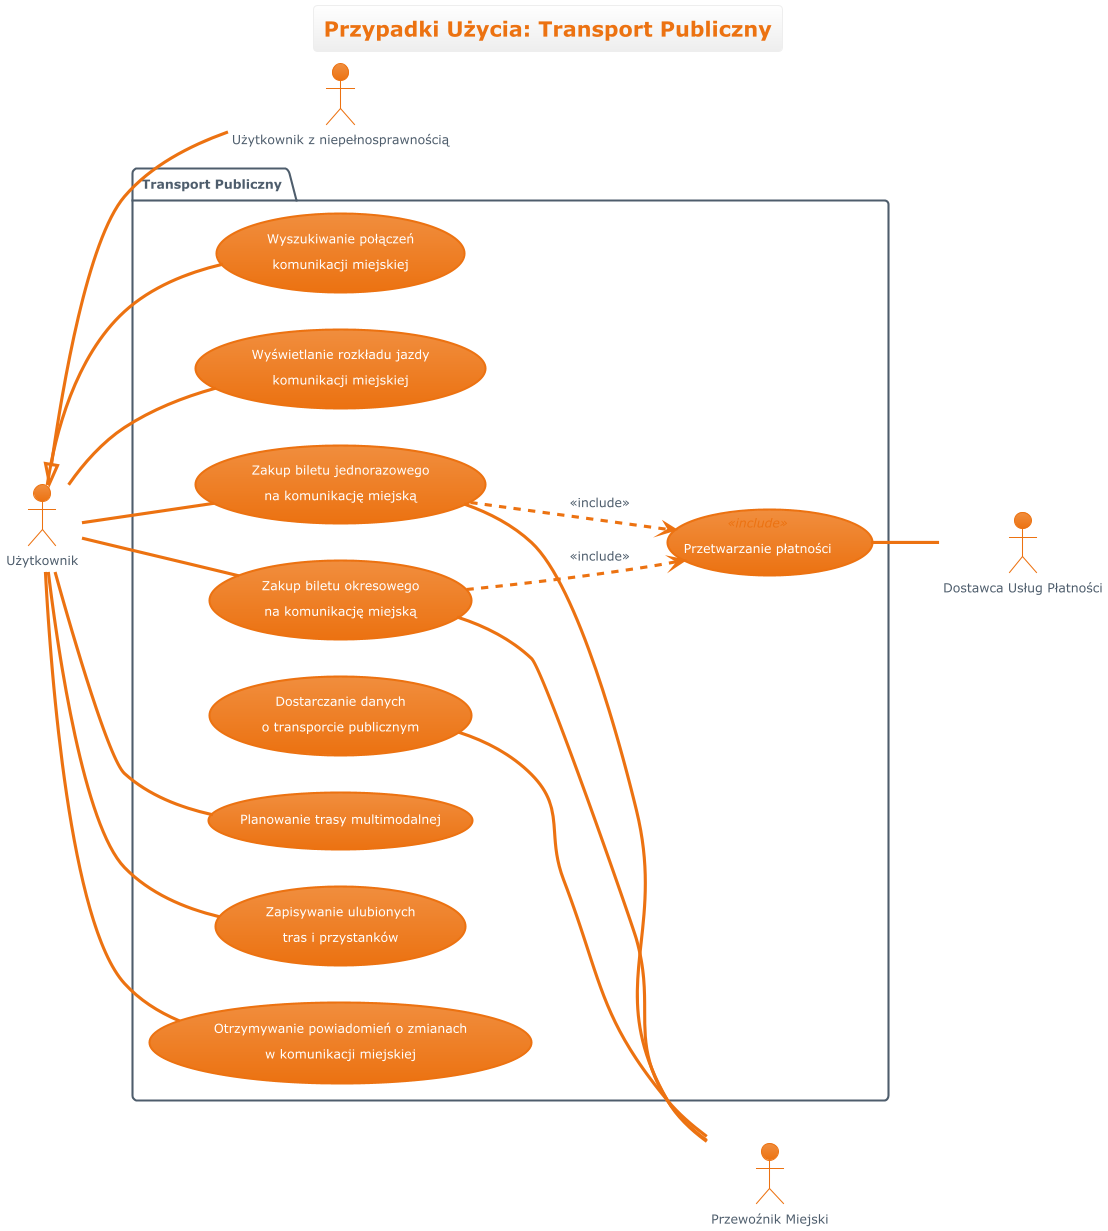
\includegraphics[width=0.9\linewidth]{diagramy/przypadki_uzycia/images/diagram_transport_publiczny.png}
    \caption{Diagram przypadków użycia: Transport publiczny}
    \label{fig:diag_tp}
\end{figure}

\subsubsection{Przejazdy Taksówką / Na Żądanie}
\begin{enumerate}[label=\arabic*.]
    \item Zamawianie przejazdu (Użytkownik, Przewoźnik Prywatny, Dostawca Usług Płatności)
    \item Rezerwacja przyszłego przejazdu (Użytkownik, Kierowca, Przewoźnik Prywatny, Dostawca Usług Płatności)
    \item Śledzenie lokalizacji zamówionego pojazdu (Użytkownik, Kierowca)
    \item Anulowanie zamówionego przejazdu (Użytkownik, Kierowca, Przewoźnik Prywatny, Dostawca Usług Płatności)
    \item Ocena kierowcy i przejazdu (Użytkownik)
    \item Otrzymywanie powiadomienia o przyjeździe pojazdu (Użytkownik)
    \item Akceptacja lub odrzucenie zlecenia (Kierowca, Przewoźnik Prywatny)
    \item Nawigowanie do miejsca odbioru pasażera (Kierowca)
    \item Zgłaszanie rozpoczęcia kursu (Kierowca)
    \item Zgłaszanie zakończenia kursu (Kierowca, Dostawca Usług Płatności)
    \item Zgłaszanie gotowości do przyjmowania zleceń (Kierowca)
\end{enumerate}
\begin{figure}[H]
    \centering
    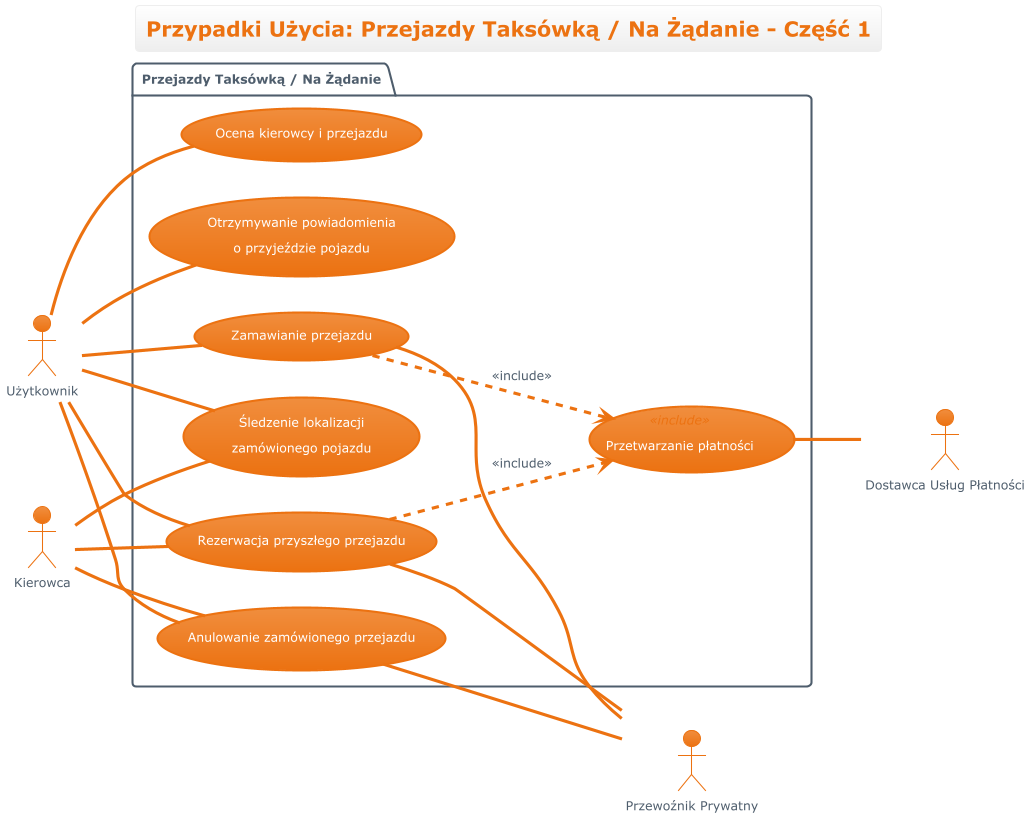
\includegraphics[width=0.8\linewidth]{diagramy/przypadki_uzycia/images/diagram_przejazdy_taksowka_1.png}
    \caption{Diagram przypadków użycia: Przejazdy taksówką / na żądanie - część 1}
    \label{fig:diag_pt_1}
\end{figure}
\begin{figure}[H]
    \centering
    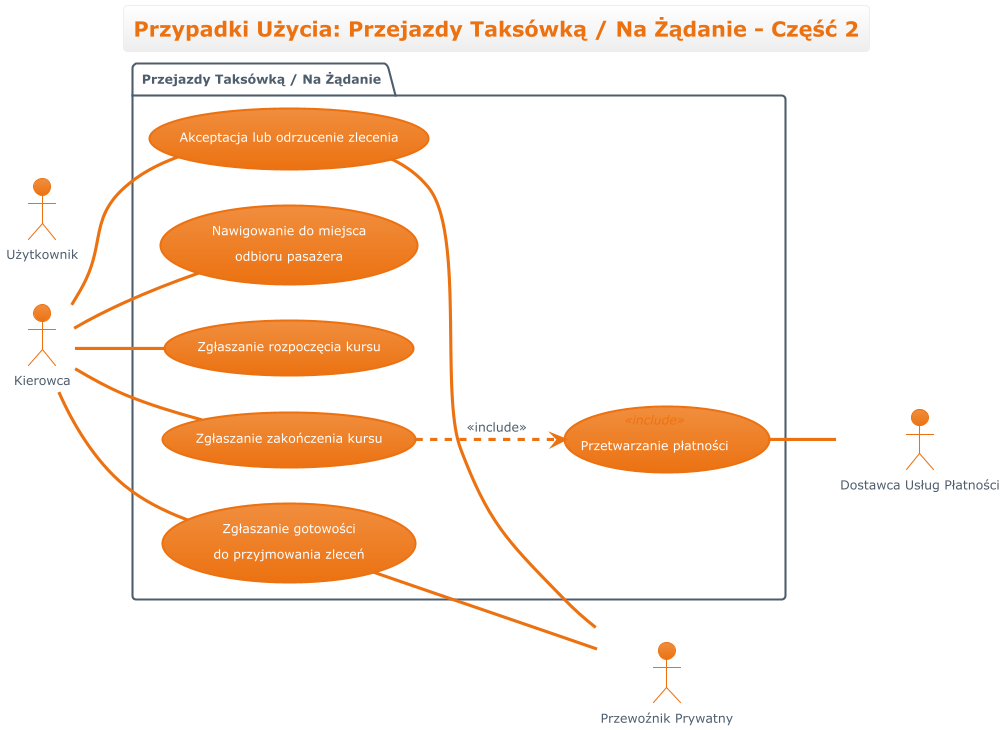
\includegraphics[width=0.8\linewidth]{diagramy/przypadki_uzycia/images/diagram_przejazdy_taksowka_2.png}
    \caption{Diagram przypadków użycia: Przejazdy taksówką / na żądanie - część 2}
    \label{fig:diag_pt_2}
\end{figure}

\subsubsection{Bilety Kolejowe}
\begin{enumerate}[label=\arabic*.]
    \item Wyszukiwanie połączeń kolejowych (Użytkownik)
    \item Wyświetlanie szczegółów połączenia kolejowego (Użytkownik)
    \item Wybór miejsca w pociągu (Użytkownik)
    \item Dodawanie danych pasażera (Użytkownik)
    \item Zakup biletu kolejowego (Użytkownik, Przewoźnik Kolejowy, Dostawca Usług Płatności)
    \item Otrzymywanie powiadomień o zmianach dotyczących podróży koleją (Użytkownik)
    \item Anulowanie biletu kolejowego (Użytkownik, Przewoźnik Kolejowy, Dostawca Usług Płatności)
    \item Wymiana biletu kolejowego (Użytkownik, Przewoźnik Kolejowy, Dostawca Usług Płatności)
    \item Pobieranie faktury za bilet kolejowy (Użytkownik)
\end{enumerate}
\begin{figure}[H]
    \centering
    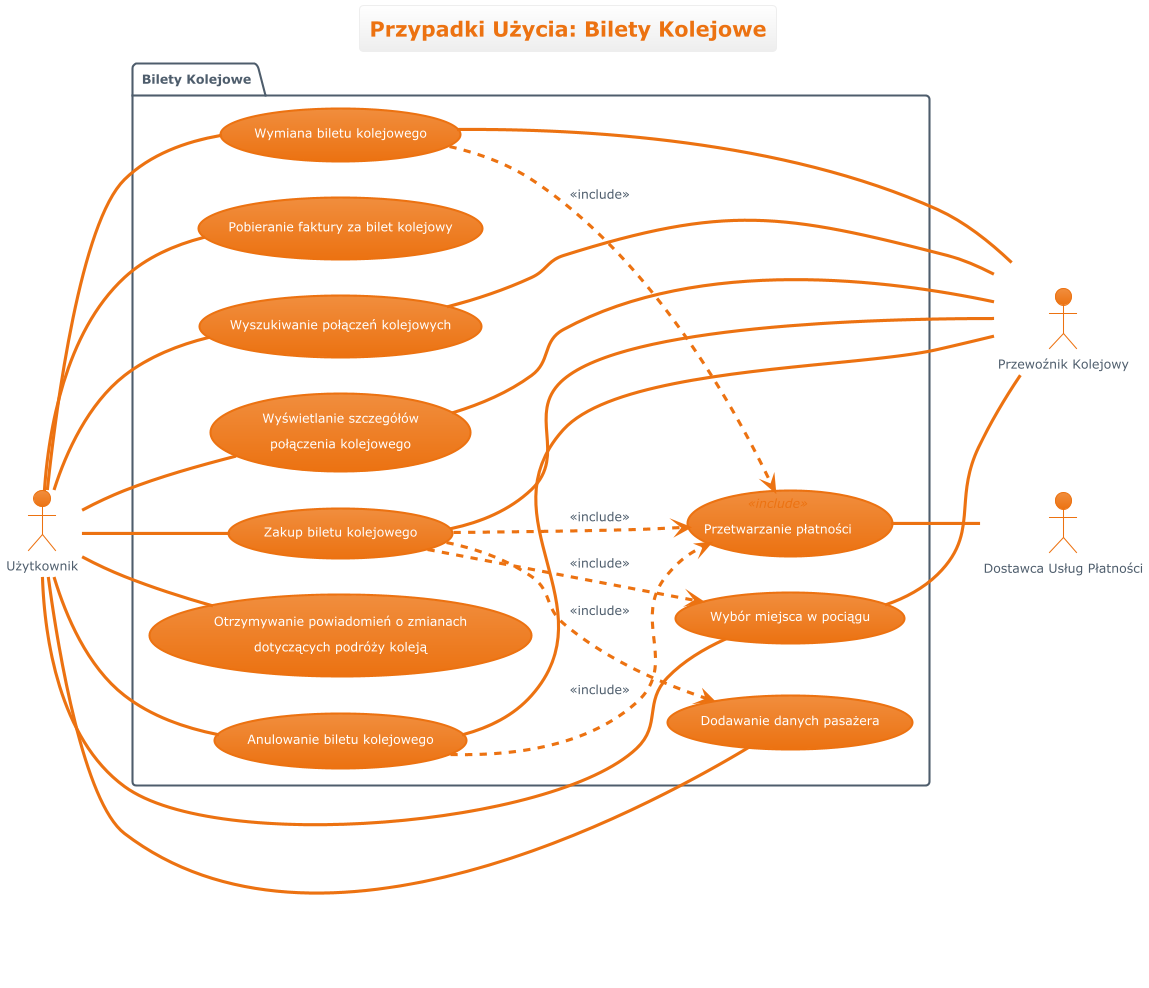
\includegraphics[width=0.8\linewidth]{diagramy/przypadki_uzycia/images/diagram_bilety_kolejowe_1.png}
    \caption{Diagram przypadków użycia: Bilety kolejowe}
    \label{fig:diag_bk_1}
\end{figure}

\subsubsection{Bilety Lotnicze}
\begin{enumerate}[label=\arabic*.]
    \item Ustawianie preferencji wyszukiwania lotów (Użytkownik)
    \item Zakup/Rezerwacja biletu lotniczego (Użytkownik, Przewoźnik lotniczy, Dostawca Usług Płatności)
    \item Wyszukiwanie połączeń lotniczych (Użytkownik)
    \item Wyświetlanie szczegółów połączenia lotniczego (Użytkownik)
    \item Porównywanie cen biletów lotniczych (Użytkownik)
    \item Dostarczanie danych o połączeniach i cenach biletów lotniczych (Przewoźnik Lotniczy)
    \item Rezerwacja transportu na/z lotniska (Użytkownik, Kierowca, Przewoźnik Prywatny, Dostawca Usług Płatności)
    \item Zarządzanie kartą pokładową (Użytkownik)
    \item Sprawdzanie statusu lotu (Użytkownik)
    \item Otrzymywanie alertów cenowych na loty (Użytkownik)
    \item Wyświetlanie mapy lotniska (Użytkownik)
\end{enumerate}
\begin{figure}[H]
    \centering
    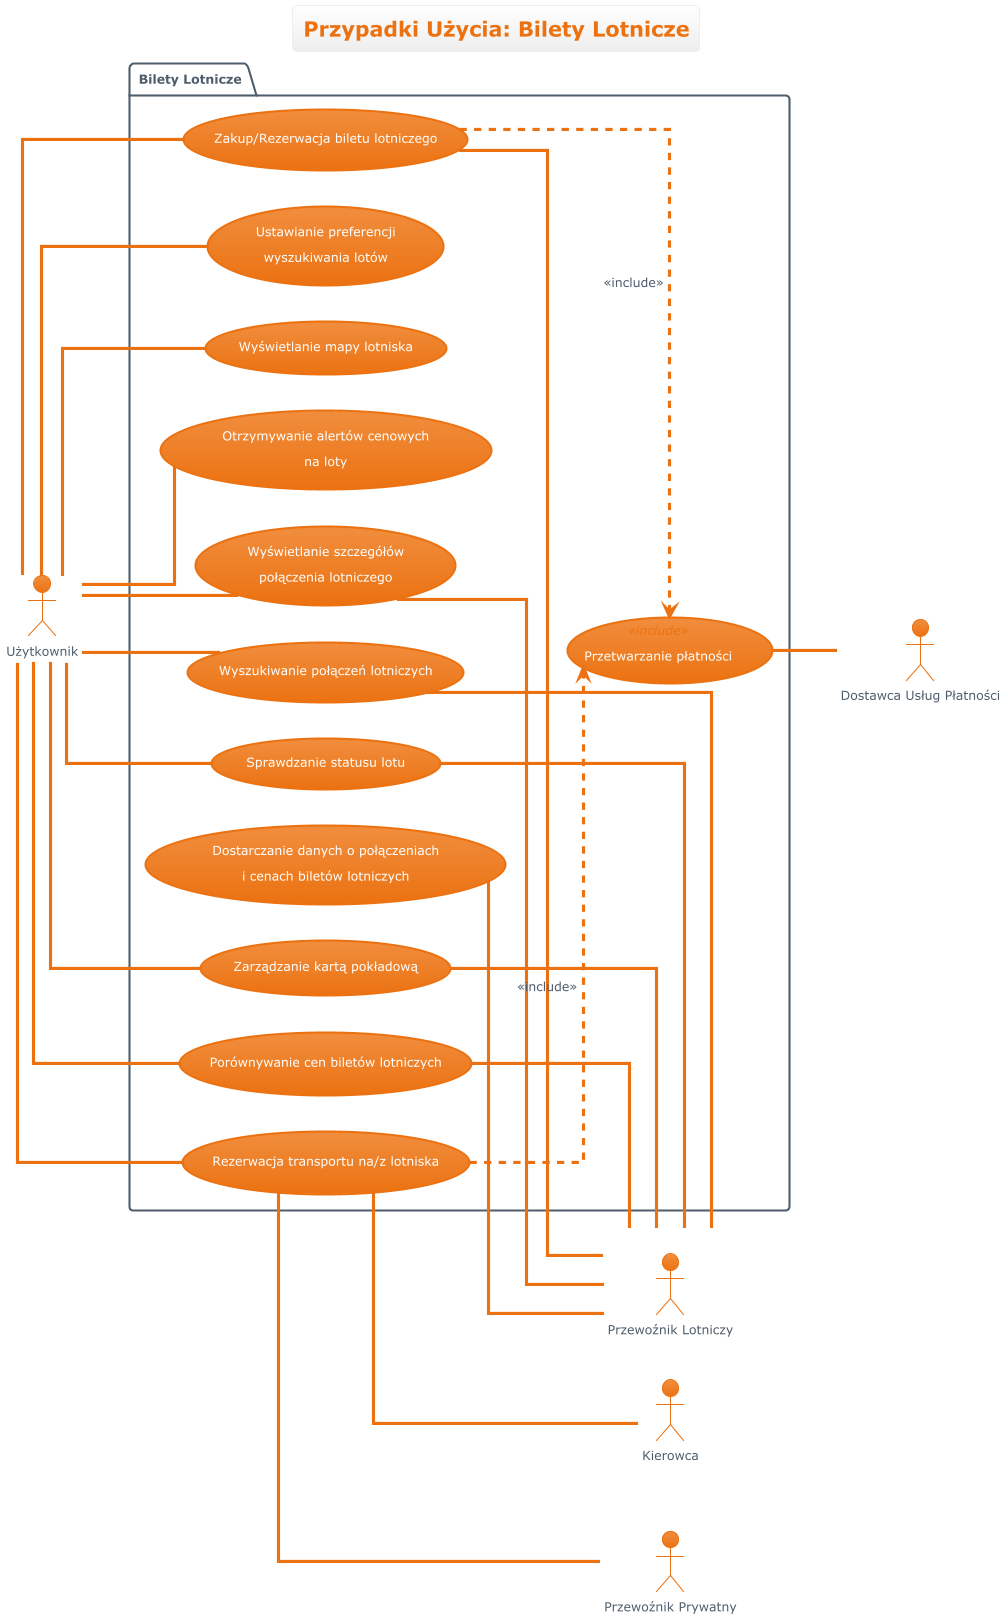
\includegraphics[width=0.8\linewidth]{diagramy/przypadki_uzycia/images/diagram_bilety_lotnicze_1.png}
    \caption{Diagram przypadków użycia: Bilety lotnicze}
    \label{fig:diag_bl_1}
\end{figure}










% POCZATEK -------------
















\newpage
\section{Scenariusze Przypadków Użycia}
\label{sec:scenarios}
Niniejszy rozdział zawiera szczegółowe scenariusze dla wybranych przypadków użycia zidentyfikowanych w systemie OpenTravel. Każdy scenariusz opisuje krok po kroku interakcję aktorów z systemem, warunki początkowe i końcowe, główny ciąg zdarzeń oraz możliwe alternatywne przebiegi i sytuacje wyjątkowe. Celem jest precyzyjne zdefiniowanie zachowania systemu w odpowiedzi na działania użytkowników i systemów zewnętrznych.


\subsection{Zarządzanie Kontem i Funkcje Ogólne}


\subsubsection{PU-ZK-01: Rejestracja w systemie}

\begingroup % Lokalny zasięg dla \small i \arraystretch
\small % Zmniejszenie czcionki w tabeli
\renewcommand{\arraystretch}{1.2} % Zmniejszona interlinia dla większej zwięzłości

% Definicja szerokości pierwszej kolumny
\newlength{\pierwszakolumnaszerokoscPUZKDetailShort} % Nowa unikalna nazwa
\setlength{\pierwszakolumnaszerokoscPUZKDetailShort}{4.0cm} % Możesz dostosować tę szerokość

% Definicja szerokości drugiej kolumny (obliczana)
\newlength{\drugakolumnaszerokoscPUZKDetailShort} % Nowa unikalna nazwa
\setlength{\drugakolumnaszerokoscPUZKDetailShort}{\dimexpr\textwidth-\pierwszakolumnaszerokoscPUZKDetailShort-2\tabcolsep-3\arrayrulewidth\relax}


\begin{longtable}{|p{\pierwszakolumnaszerokoscPUZKDetailShort}|p{\drugakolumnaszerokoscPUZKDetailShort}|}
    \caption{Scenariusz przypadku użycia: PU-ZK-01 Rejestracja w systemie}\\ 
    \hline
    \textbf{Element} & \textbf{Opis} \\
    \hline
    \endfirsthead 

    \multicolumn{2}{c}%
    {{\bfseries\tablename\ \thetable} -- \textit{kontynuacja z poprzedniej strony}} \\
    \hline
    \textbf{Element} & \textbf{Opis} \\
    \hline
    \endhead 

    \hline
    \multicolumn{2}{r}{{\textit{Ciąg dalszy na następnej stronie}}} \\
    \endfoot 

    \hline
    \endlastfoot 

    % --- Początek MAKSYMALNIE SKRÓCONEJ I UZUPEŁNIONEJ treści tabeli ---
    \textbf{Aktorzy} & Nowy Użytkownik, Nowy Kierowca. \\
    \hline
    \textbf{Zakres} & Utworzenie konta Użytkownika/Kierowcy w OpenTravel. \\
    \hline
    \textbf{Poziom} & Cel użytkownika. \\
    \hline
    \textbf{Udziałowcy i ich cele} & 
        \begin{itemize} \itemsep0pt \parskip0pt \parsep0pt
            \item \textit{Aktor:} Dostęp do funkcji systemu.
            \item \textit{System:} Pozyskanie zweryfikowanych użytkowników.
        \end{itemize} \\
    \hline
    \textbf{Zdarzenie wyzwalające} & Aktor wybiera opcję "Rejestracja". \\
    \hline
    \textbf{Warunki wstępne} & 
        \begin{itemize} \itemsep0pt \parskip0pt \parsep0pt
            \item Dostęp do interfejsu rejestracji.
            \item Brak istniejącego konta.
            \item Działający system i adres e-mail Aktora.
        \end{itemize} \\
    \hline
    \textbf{Warunki końcowe dla sukcesu} & 
        \begin{itemize} \itemsep0pt \parskip0pt \parsep0pt
            \item Konto Aktora utworzone, dane zapisane.
            \item Otrzymano e-mail potwierdzający/aktywacyjny.
            \item Możliwość logowania po weryfikacji e-mail.
            \item Konto Kierowcy może wymagać dodatkowej weryfikacji przez Administratora.
        \end{itemize} \\
    \hline
    \textbf{Warunki końcowe dla niepowodzenia} & 
        \begin{itemize} \itemsep0pt \parskip0pt \parsep0pt
            \item Konto nieutworzone.
            \item Komunikat o błędzie dla Aktora.
        \end{itemize} \\
    \hline
    \textbf{Scenariusz główny} & 
        \textbf{Dla Nowego Użytkownika:}
        \begin{enumerate} \itemsep0pt \parskip0pt \parsep0pt
            \item Aktor wybiera "Rejestracja", wypełnia formularz (e-mail, hasło, dane os.), akceptuje warunki.
            \item System waliduje dane.
            \item Jeśli OK: tworzy konto, wysyła e-mail aktywacyjny.
            \item Aktor klika link aktywacyjny; konto aktywne.
        \end{enumerate}
        \vspace{0.3em} % Minimalny odstęp
        \textbf{Dla Nowego Kierowcy:}
        \begin{enumerate} \itemsep0pt \parskip0pt \parsep0pt
            \item Aktor wybiera "Rejestracja jako Kierowca", wypełnia formularz (dane jak Użytkownik + ew. dane dot. uprawnień/pojazdu/dokumentów), akceptuje warunki.
            \item System waliduje dane.
            \item Jeśli OK: tworzy konto (status np. "Oczekuje na weryfikację"), wysyła e-mail (np. z linkiem aktywacyjnym i info o dalszych krokach).
            \item Aktor weryfikuje e-mail (jeśli wymagane). Konto oczekuje na weryfikację dokumentów/aktywację przez Administratora.
        \end{enumerate} \\
    \hline
    \textbf{Scenariusze alternatywne} & 
        \begin{itemize} \itemsep0pt \parskip0pt \parsep0pt
            \item \textbf{A1: Rejestracja przez konto zewnętrzne (np. Google):} Aktor autoryzuje przez zewn. dostawcę; system pobiera dane; Aktor uzupełnia/akceptuje.
            \item \textbf{A2: Brak akceptacji regulaminu:} Rejestracja wstrzymana.
        \end{itemize} \\
    \hline
    \textbf{Sytuacje wyjątkowe (Przykłady)} & 
        \begin{itemize} \itemsep0pt \parskip0pt \parsep0pt
            \item \textbf{W1: E-mail zajęty:} Komunikat, sugestia logowania/zmiany.
            \item \textbf{W2: Błędne hasło/dane:} Komunikat o błędzie, wymóg poprawy.
            \item \textbf{W3: Błąd systemowy (e-mail/baza):} Komunikat o błędzie tech.
        \end{itemize} \\
\end{longtable}
\endgroup


% DRUGI --------------

\subsubsection{PU-ZK-02: Logowanie do systemu}

\begingroup % Lokalny zasięg dla \small i \arraystretch
\small % Zmniejszenie czcionki w tabeli
\renewcommand{\arraystretch}{1.3} % Dostosowanie interlinii dla czytelności

% Definicja szerokości pierwszej kolumny
\newlength{\pierwszakolumnaszerokoscPUZKLog} % Unikalna nazwa dla tej tabeli
\setlength{\pierwszakolumnaszerokoscPUZKLog}{3.8cm} % Możesz dostosować tę szerokość

% Definicja szerokości drugiej kolumny (obliczana)
\newlength{\drugakolumnaszerokoscPUZKLog} % Unikalna nazwa
\setlength{\drugakolumnaszerokoscPUZKLog}{\dimexpr\textwidth-\pierwszakolumnaszerokoscPUZKLog-2\tabcolsep-3\arrayrulewidth\relax}


\begin{longtable}{|p{\pierwszakolumnaszerokoscPUZKLog}|p{\drugakolumnaszerokoscPUZKLog}|}
    \caption{Scenariusz przypadku użycia: PU-ZK-02 Logowanie do systemu }\\ 
    \hline
    \textbf{Element} & \textbf{Opis} \\
    \hline
    \endfirsthead 

    \multicolumn{2}{c}%
    {{\bfseries\tablename\ \thetable} -- \textit{kontynuacja z poprzedniej strony}} \\
    \hline
    \textbf{Element} & \textbf{Opis} \\
    \hline
    \endhead 

    \hline
    \multicolumn{2}{r}{{\textit{Ciąg dalszy na następnej stronie}}} \\
    \endfoot 

    \hline
    \endlastfoot 

    % --- Początek SKRÓCONEJ treści tabeli dla Logowania ---
    \textbf{Aktorzy} & Użytkownik, Administrator systemu, Kierowca (dalej: Zarejestrowany Aktor). \\
    \hline
    \textbf{Zakres} & Umożliwienie Zarejestrowanemu Aktorowi dostępu do systemu OpenTravel po weryfikacji tożsamości. \\
    \hline
    \textbf{Poziom} & Cel użytkownika / Funkcja systemowa. \\
    \hline
    \textbf{Udziałowcy i ich cele} & 
        \begin{itemize} \itemsep0pt \parskip0pt \parsep0pt
            \item \textit{Zarejestrowany Aktor:} Dostęp do spersonalizowanych funkcji i danych.
            \item \textit{System OpenTravel:} Zapewnienie bezpiecznego dostępu tylko autoryzowanym aktorom.
        \end{itemize} \\
    \hline
    \textbf{Zdarzenie wyzwalające} & Aktor wybiera "Logowanie" i wprowadza dane uwierzytelniające. \\
    \hline
    \textbf{Warunki wstępne} & 
        \begin{itemize} \itemsep0pt \parskip0pt \parsep0pt
            \item Aktor posiada aktywne konto w systemie.
            \item Aktor zna swoje dane logowania (np. e-mail/login i hasło).
            \item Dostępny interfejs logowania i działający system.
        \end{itemize} \\
    \hline
    \textbf{Warunki końcowe dla sukcesu} & 
        \begin{itemize} \itemsep0pt \parskip0pt \parsep0pt
            \item Aktor jest zalogowany do systemu.
            \item Ustanowiona aktywna sesja dla Aktora.
            \item Dostęp do funkcji zgodnych z uprawnieniami Aktora.
        \end{itemize} \\
    \hline
    \textbf{Warunki końcowe dla niepowodzenia} & 
        \begin{itemize} \itemsep0pt \parskip0pt \parsep0pt
            \item Aktor nie jest zalogowany.
            \item System wyświetla komunikat o błędzie logowania.
        \end{itemize} \\
    \hline
    \textbf{Scenariusz główny} & 
        \begin{enumerate} \itemsep0pt \parskip0pt \parsep0pt
            \item Aktor wybiera opcję "Logowanie".
            \item System wyświetla formularz (e-mail/login, hasło).
            \item Aktor wprowadza dane uwierzytelniające i zatwierdza.
            \item System weryfikuje poprawność danych z bazą.
            \item Dane poprawne: System ustanawia sesję, Aktor uzyskuje dostęp do panelu/widoku zgodnego z rolą.
        \end{enumerate} \\
    \hline
    \textbf{Scenariusze alternatywne} & 
        \begin{itemize} \itemsep0pt \parskip0pt \parsep0pt
            \item \textbf{A1: Logowanie przez konto zewnętrzne (np. Google):} Aktor wybiera opcję; po autoryzacji u dostawcy zewn., system loguje Aktora.
            \item \textbf{A2: Opcja "Zapamiętaj mnie":} Aktor zaznacza; system ułatwia przyszłe logowania (np. przez token).
            \item \textbf{A3: Aktor wybiera "Odzyskaj hasło":} Przejście do przypadku użycia PU-ZK-04 Odzyskiwanie hasła.
        \end{itemize} \\
    \hline
    \textbf{Sytuacje wyjątkowe (Przykłady)} & 
        \begin{itemize} \itemsep0pt \parskip0pt \parsep0pt
            \item \textbf{W1: Błędne dane logowania:} Komunikat "Nieprawidłowe dane logowania". Możliwość ponowienia.
            \item \textbf{W2: Konto nieaktywne/zablokowane:} Komunikat o statusie konta; info o krokach do aktywacji/odblokowania.
            \item \textbf{W3: Przekroczono limit prób logowania:} Tymczasowa blokada logowania (np. dla konta/IP).
            \item \textbf{W4: Błąd systemowy podczas logowania:} Komunikat o błędzie technicznym.
        \end{itemize} \\
    % --- Koniec SKRÓCONEJ treści tabeli dla Logowania ---
\end{longtable}
\endgroup



% Trzeci 

\subsubsection{PU-ZK-03: Zarządzanie danymi konta}

\begingroup % Lokalny zasięg dla \small i \arraystretch
\small % Zmniejszenie czcionki w tabeli
\renewcommand{\arraystretch}{1.3} % Dostosowanie interlinii dla czytelności

% Definicja szerokości pierwszej kolumny
\newlength{\pierwszakolumnaszerokoscPUZKDaneShort} 
\setlength{\pierwszakolumnaszerokoscPUZKDaneShort}{4.2cm} % Możesz dostosować tę szerokość

% Definicja szerokości drugiej kolumny (obliczana)
\newlength{\drugakolumnaszerokoscPUZKDaneShort} 
\setlength{\drugakolumnaszerokoscPUZKDaneShort}{\dimexpr\textwidth-\pierwszakolumnaszerokoscPUZKDaneShort-2\tabcolsep-3\arrayrulewidth\relax}


\begin{longtable}{|p{\pierwszakolumnaszerokoscPUZKDaneShort}|p{\drugakolumnaszerokoscPUZKDaneShort}|}
    \caption{Scenariusz przypadku użycia: PU-ZK-03 Zarządzanie danymi konta}\\ 
    \hline
    \textbf{Element} & \textbf{Opis} \\
    \hline
    \endfirsthead 

    \multicolumn{2}{c}%
    {{\bfseries\tablename\ \thetable} -- \textit{kontynuacja z poprzedniej strony}} \\
    \hline
    \textbf{Element} & \textbf{Opis} \\
    \hline
    \endhead 

    \hline
    \multicolumn{2}{r}{{\textit{Ciąg dalszy na następnej stronie}}} \\
    \endfoot 

    \hline
    \endlastfoot 

    % --- Początek SKRÓCONEJ treści tabeli ---
    \textbf{Aktorzy} & Użytkownik, Administrator systemu, Kierowca. \\
    \hline
    \textbf{Zakres} & Umożliwia Aktorom przeglądanie i modyfikację danych konta; Administrator zarządza kontami użytkowników. \\
    \hline
    \textbf{Poziom} & Cel użytkownika / Funkcja systemowa. \\
    \hline
    \textbf{Udziałowcy i ich cele} & 
        \begin{itemize} \itemsep0pt \parskip0pt \parsep0pt
            \item \textit{Aktor (Użytkownik/Kierowca):} Aktualizacja danych, zarządzanie bezpieczeństwem (hasło), personalizacja.
            \item \textit{Administrator:} Zarządzanie kontami, integralność danych, wsparcie.
            \item \textit{System:} Bezpieczne zarządzanie aktualnymi danymi kont.
        \end{itemize} \\
    \hline
    \textbf{Zdarzenie wyzwalające} & 
        \begin{itemize} \itemsep0pt \parskip0pt \parsep0pt
            \item \textit{Aktor (Użytkownik/Kierowca):} Wybiera opcję "Ustawienia".
            \item \textit{Administrator:} Wybiera zarządzanie użytkownikami i konkretne konto.
        \end{itemize} \\
    \hline
    \textbf{Warunki wstępne} & 
        \begin{itemize} \itemsep0pt \parskip0pt \parsep0pt
            \item Aktor zalogowany do systemu.
            \item System dostępny.
            \item Administrator ma odpowiednie uprawnienia.
        \end{itemize} \\
    \hline
    \textbf{Warunki końcowe dla sukcesu} & 
        \begin{itemize} \itemsep0pt \parskip0pt \parsep0pt
            \item Dane konta zaktualizowane (jeśli były modyfikacje).
            \item Aktor widzi zmiany w profilu.
            \item Administrator wykonał operacje zarządcze.
            \item Zmiany zapisane w bazie danych.
        \end{itemize} \\
    \hline
    \textbf{Warunki końcowe dla niepowodzenia} & 
        \begin{itemize} \itemsep0pt \parskip0pt \parsep0pt
            \item Zmiany nie zostały zapisane (błąd walidacji).
            \item Aktor otrzymuje komunikat o błędzie.
            \item System pozostaje w spójnym stanie.
        \end{itemize} \\
    \hline
    \textbf{Scenariusz główny} & 
        \textbf{Dla Użytkownika/Kierowcy (modyfikacja własnych danych):}
        \begin{enumerate} \itemsep0pt \parskip0pt \parsep0pt
            \item Aktor przechodzi do sekcji zarządzania kontem.
            \item System wyświetla dane konta (dane os., kontaktowe, hasło, preferencje; Kierowca: dane pojazdu/dokumenty).
            \item Aktor wybiera dane do edycji, wprowadza zmiany, zatwierdza.
            \item System waliduje i zapisuje zmiany. Wyświetla potwierdzenie.
        \end{enumerate}
        \vspace{0.5em}
        \textbf{Dla Administratora systemu (zarządzanie kontem):}
        \begin{enumerate} \itemsep0pt \parskip0pt \parsep0pt
            \item Administrator loguje się, wyszukuje i wybiera konto.
            \item System wyświetla dane konta i opcje zarządcze (np. zmiana statusu, reset hasła, edycja uprawnień).
            \item Administrator wybiera akcję, potwierdza (jeśli wymagane).
            \item System wykonuje akcję, zapisuje zmiany, wyświetla potwierdzenie.
        \end{enumerate} \\
    \hline
    \textbf{Scenariusze alternatywne} & 
        \begin{itemize} \itemsep0pt \parskip0pt \parsep0pt
            \item \textbf{A1: (Użytkownik/Kierowca) Zmiana hasła:} Aktor wybiera opcję, podaje stare i nowe hasło (z potwierdzeniem); system weryfikuje i aktualizuje.
            \item \textbf{A2: (Użytkownik/Kierowca) Anulowanie edycji:} Zmiany przed zapisem są odrzucane, dane pozostają niezmienione.
            \item \textbf{A3: (Kierowca) Aktualizacja danych pojazdu/dokumentów:} Kierowca aktualizuje specyficzne dane; mogą podlegać weryfikacji przez Administratora.
        \end{itemize} \\
    \hline
    \textbf{Sytuacje wyjątkowe (Przykłady)} & 
        \begin{itemize} \itemsep0pt \parskip0pt \parsep0pt
            \item \textbf{W1: Nieudana walidacja danych (format, polityka):} Komunikat błędu, zmiany niezapisane.
            \item \textbf{W2: (Zmiana hasła) Błędne stare hasło:} Komunikat, zmiana niemożliwa.
            \item \textbf{W3: (Administrator) Brak uprawnień do akcji:} Akcja zablokowana, komunikat.
            \item \textbf{W4: Błąd zapisu do bazy / Błąd systemowy:} Komunikat o błędzie technicznym.
            \item \textbf{W5: E-mail już w użyciu (przy próbie zmiany na istniejący):} Komunikat o konflikcie.
        \end{itemize} \\
    % --- Koniec SKRÓCONEJ treści tabeli ---
\end{longtable}
\endgroup


% Czwarty

\subsubsection{PU-ZK-04: Odzyskiwanie hasła}

\begingroup % Lokalny zasięg dla \small i \arraystretch
\small % Zmniejszenie czcionki w tabeli
\renewcommand{\arraystretch}{1.3} % Dostosowanie interlinii dla czytelności

% Definicja szerokości pierwszej kolumny
\newlength{\pierwszakolumnaszerokoscPUZKOdzysk} 
\setlength{\pierwszakolumnaszerokoscPUZKOdzysk}{4.2cm} % Możesz dostosować tę szerokość

% Definicja szerokości drugiej kolumny (obliczana)
\newlength{\drugakolumnaszerokoscPUZKOdzysk} 
\setlength{\drugakolumnaszerokoscPUZKOdzysk}{\dimexpr\textwidth-\pierwszakolumnaszerokoscPUZKOdzysk-2\tabcolsep-3\arrayrulewidth\relax}


\begin{longtable}{|p{\pierwszakolumnaszerokoscPUZKOdzysk}|p{\drugakolumnaszerokoscPUZKOdzysk}|}
    \caption{Scenariusz przypadku użycia: PU-ZK-04 Odzyskiwanie hasła}\\ 
    \hline
    \textbf{Element} & \textbf{Opis} \\
    \hline
    \endfirsthead 

    \multicolumn{2}{c}%
    {{\bfseries\tablename\ \thetable} -- \textit{kontynuacja z poprzedniej strony}} \\
    \hline
    \textbf{Element} & \textbf{Opis} \\
    \hline
    \endhead 

    \hline
    \multicolumn{2}{r}{{\textit{Ciąg dalszy na następnej stronie}}} \\
    \endfoot 

    \hline
    \endlastfoot 

    % --- Początek SKRÓCONEJ treści tabeli ---
    \textbf{Aktorzy} & Użytkownik, Kierowca, Administrator systemu. \\
    \hline
    \textbf{Zakres} & Umożliwia Użytkownikowi/Kierowcy odzyskanie/zresetowanie zapomnianego hasła. Administrator może inicjować reset hasła dla użytkowników. \\
    \hline
    \textbf{Poziom} & Cel użytkownika / Funkcja systemowa. \\
    \hline
    \textbf{Udziałowcy i ich cele} & 
        \begin{itemize} \itemsep0pt \parskip0pt \parsep0pt
            \item \textit{Użytkownik/Kierowca:} Odzyskanie dostępu do konta.
            \item \textit{Administrator:} Pomoc użytkownikom w odzyskaniu dostępu, zarządzanie bezpieczeństwem.
            \item \textit{System OpenTravel:} Zapewnienie bezpiecznego mechanizmu resetowania haseł.
        \end{itemize} \\
    \hline
    \textbf{Zdarzenie wyzwalające} & 
        \begin{itemize} \itemsep0pt \parskip0pt \parsep0pt
            \item \textit{Użytkownik/Kierowca:} Wybiera opcję "Zapomniałem hasła" na ekranie logowania.
            \item \textit{Administrator:} Inicjuje reset hasła dla użytkownika z panelu administracyjnego.
        \end{itemize} \\
    \hline
    \textbf{Warunki wstępne} & 
        \begin{itemize} \itemsep0pt \parskip0pt \parsep0pt
            \item \textit{Użytkownik/Kierowca:} Posiada konto z zarejestrowanym adresem e-mail.
            \item System dostępny, usługa e-mail działa.
            \item \textit{Administrator:} Zalogowany, posiada odpowiednie uprawnienia.
        \end{itemize} \\
    \hline
    \textbf{Warunki końcowe dla sukcesu} & 
        \begin{itemize} \itemsep0pt \parskip0pt \parsep0pt
            \item \textit{Użytkownik/Kierowca:} Pomyślnie ustawił nowe hasło i może zalogować się na konto.
            \item \textit{Dla akcji Admina:} Użytkownik otrzymał instrukcje/link do resetu hasła.
            \item Bezpieczeństwo konta jest zachowane poprzez zmianę hasła.
        \end{itemize} \\
    \hline
    \textbf{Warunki końcowe dla niepowodzenia} & 
        \begin{itemize} \itemsep0pt \parskip0pt \parsep0pt
            \item Hasło nie zostało zmienione; Aktor nie odzyskał dostępu.
            \item Wyświetlono komunikat o błędzie.
        \end{itemize} \\
    \hline
    \textbf{Scenariusz główny} & 
        \textbf{Dla Użytkownika/Kierowcy:}
        \begin{enumerate} \itemsep0pt \parskip0pt \parsep0pt
            \item Aktor wybiera "Zapomniałem hasła".
            \item System prosi o podanie adresu e-mail konta. Aktor podaje e-mail.
            \item System weryfikuje e-mail; jeśli istnieje, wysyła e-mail z linkiem/kodem do resetu. Informuje Aktora.
            \item Aktor odbiera e-mail, używa linku/kodu.
            \item System wyświetla formularz ustawienia nowego hasła.
            \item Aktor wprowadza i zatwierdza nowe hasło (zgodne z polityką).
            \item System zapisuje nowe hasło, informuje o sukcesie.
        \end{enumerate}
        \vspace{0.5em}
        \textbf{Dla Administratora systemu (inicjowanie resetu):}
        \begin{enumerate} \itemsep0pt \parskip0pt \parsep0pt
            \item Admin w panelu wybiera użytkownika i opcję "Resetuj hasło".
            \item System generuje tymczasowe hasło lub wysyła link do resetu na e-mail użytkownika.
            \item System informuje Admina o akcji; użytkownik kończy proces.
        \end{enumerate} \\
    \hline
    \textbf{Scenariusze alternatywne} & 
        \begin{itemize} \itemsep0pt \parskip0pt \parsep0pt
            \item \textbf{A1: Odzyskiwanie przez pytanie bezpieczeństwa (jeśli zaimplementowane):} Po podaniu e-maila, system zadaje pytanie bezp.; poprawna odpowiedź prowadzi do resetu.
            \item \textbf{A2: Użytkownik/Kierowca rezygnuje z procesu:} Aktor zamyka formularz przed ustawieniem nowego hasła; hasło pozostaje niezmienione.
        \end{itemize} \\
    \hline
    \textbf{Sytuacje wyjątkowe (Przykłady)} & 
        \begin{itemize} \itemsep0pt \parskip0pt \parsep0pt
            \item \textbf{W1: E-mail nie istnieje w systemie:} Komunikat "Brak konta dla podanego adresu e-mail".
            \item \textbf{W2: Link/kod do resetu nieprawidłowy/wygasł:} Komunikat błędu, sugestia ponowienia.
            \item \textbf{W3: Nowe hasło nie spełnia polityki bezpieczeństwa:} Komunikat, wymóg poprawy.
            \item \textbf{W4: Błąd wysyłki e-maila z linkiem/kodem:} Komunikat o błędzie technicznym.
        \end{itemize} \\
\end{longtable}
\endgroup



% PIĄTY

\subsubsection{PU-ZK-05: Zarządzanie metodami płatności}

\begingroup % Lokalny zasięg dla \small i \arraystretch
\small % Zmniejszenie czcionki w tabeli
\renewcommand{\arraystretch}{1.3} % Dostosowanie interlinii dla czytelności

% Definicja szerokości pierwszej kolumny
\newlength{\pierwszakolumnaszerokoscPUZKPlat} 
\setlength{\pierwszakolumnaszerokoscPUZKPlat}{4.2cm} 

% Definicja szerokości drugiej kolumny (obliczana)
\newlength{\drugakolumnaszerokoscPUZKPlat} 
\setlength{\drugakolumnaszerokoscPUZKPlat}{\dimexpr\textwidth-\pierwszakolumnaszerokoscPUZKPlat-2\tabcolsep-3\arrayrulewidth\relax}


\begin{longtable}{|p{\pierwszakolumnaszerokoscPUZKPlat}|p{\drugakolumnaszerokoscPUZKPlat}|}
    \caption{Scenariusz przypadku użycia: PU-ZK-05 Zarządzanie metodami płatności}\\ 
    \hline
    \textbf{Element} & \textbf{Opis} \\
    \hline
    \endfirsthead 

    \multicolumn{2}{c}%
    {{\bfseries\tablename\ \thetable} -- \textit{kontynuacja z poprzedniej strony}} \\
    \hline
    \textbf{Element} & \textbf{Opis} \\
    \hline
    \endhead 

    \hline
    \multicolumn{2}{r}{{\textit{Ciąg dalszy na następnej stronie}}} \\
    \endfoot 

    \hline
    \endlastfoot 

    % --- Początek SKRÓCONEJ treści tabeli ---
    \textbf{Aktorzy} & Użytkownik. \\
    \hline
    \textbf{Zakres} & Umożliwia Użytkownikowi dodawanie, przeglądanie, usuwanie oraz ustawianie domyślnej metody płatności (np. karty płatniczej) w systemie OpenTravel. \\
    \hline
    \textbf{Poziom} & Cel użytkownika / Funkcja systemowa. \\
    \hline
    \textbf{Udziałowcy i ich cele} & 
        \begin{itemize} \itemsep0pt \parskip0pt \parsep0pt
            \item \textit{Użytkownik:} Wygodne i bezpieczne zarządzanie środkami płatniczymi do transakcji w systemie.
            \item \textit{System OpenTravel:} Zapewnienie bezpiecznego przechowywania (tokenizacji) danych płatniczych, ułatwienie płatności.
            \item \textit{Dostawca Usług Płatności:} Przetwarzanie transakcji.
        \end{itemize} \\
    \hline
    \textbf{Zdarzenie wyzwalające} & Użytkownik wybiera opcję "Metody płatności" / "Portfel" w ustawieniach swojego konta. \\
    \hline
    \textbf{Warunki wstępne} & 
        \begin{itemize} \itemsep0pt \parskip0pt \parsep0pt
            \item Użytkownik jest zalogowany do systemu OpenTravel.
            \item System jest zintegrowany z Dostawcą Usług Płatności.
        \end{itemize} \\
    \hline
    \textbf{Warunki końcowe dla sukcesu} & 
        \begin{itemize} \itemsep0pt \parskip0pt \parsep0pt
            \item \textit{(Dodawanie):} Nowa metoda płatności dodana, zweryfikowana i zapisana/ztokenizowana.
            \item \textit{(Usuwanie):} Wybrana metoda płatności usunięta z konta.
            \item \textit{(Ustawianie domyślnej):} Metoda ustawiona jako domyślna.
            \item Użytkownik widzi zaktualizowaną listę metod płatności.
        \end{itemize} \\
    \hline
    \textbf{Warunki końcowe dla niepowodzenia} & 
        \begin{itemize} \itemsep0pt \parskip0pt \parsep0pt
            \item Operacja na metodzie płatności nie powiodła się.
            \item Wyświetlono komunikat o błędzie.
        \end{itemize} \\
    \hline
    \textbf{Scenariusz główny} & 
        \textbf{Dodawanie nowej metody (np. karty):}
        \begin{enumerate} \itemsep0pt \parskip0pt \parsep0pt
            \item Użytkownik wybiera "Dodaj nową metodę płatności".
            \item System wyświetla formularz danych karty (nr, data ważności, CVV, etc.). Użytkownik wprowadza dane.
            \item System (przez Dostawcę Usług Płatności) weryfikuje i autoryzuje kartę (np. micro-transakcja, 3D Secure).
            \item Po pomyślnej weryfikacji, metoda jest dodawana. System potwierdza.
        \end{enumerate}
        \vspace{0.3em}
        \textbf{Przeglądanie metod:}
        \begin{enumerate} \itemsep0pt \parskip0pt \parsep0pt
            \item Użytkownik wchodzi do sekcji metod płatności.
            \item System wyświetla listę zapisanych metod (np. zamaskowane numery kart).
        \end{enumerate}
        \vspace{0.3em}
        \textbf{Usuwanie metody:}
        \begin{enumerate} \itemsep0pt \parskip0pt \parsep0pt
            \item Użytkownik wybiera metodę i opcję "Usuń". Potwierdza.
            \item System usuwa metodę z konta. System potwierdza.
        \end{enumerate}
        \vspace{0.3em}
        \textbf{Ustawianie domyślnej metody:}
        \begin{enumerate} \itemsep0pt \parskip0pt \parsep0pt
            \item Użytkownik wybiera metodę i opcję "Ustaw jako domyślną".
            \item System oznacza metodę jako domyślną. System potwierdza.
        \end{enumerate} \\
    \hline
    \textbf{Scenariusze alternatywne} & 
        \begin{itemize} \itemsep0pt \parskip0pt \parsep0pt
            \item \textbf{A1: Edycja danych metody (np. daty ważności - jeśli wspierane):} Użytkownik edytuje, system weryfikuje.
            \item \textbf{A2: Dodawanie innego typu metody (np. PayPal - jeśli wspierane):} Proces specyficzny dla danego typu (np. przekierowanie).
        \end{itemize} \\
    \hline
    \textbf{Sytuacje wyjątkowe (Przykłady)} & 
        \begin{itemize} \itemsep0pt \parskip0pt \parsep0pt
            \item \textbf{W1: Nieudana weryfikacja nowej metody:} Komunikat błędu od Dostawcy; metoda nie jest dodawana.
            \item \textbf{W2: Niepoprawne dane metody:} Komunikat o błędzie walidacji.
            \item \textbf{W3: Próba usunięcia jedynej/wymaganej metody:} System uniemożliwia lub ostrzega.
            \item \textbf{W4: Błąd komunikacji z Dostawcą Usług Płatności:} Komunikat o błędzie technicznym.
        \end{itemize} \\
\end{longtable}
\endgroup


% SZOSTY

\subsubsection{PU-ZK-06: Dodawanie zniżek do konta}

\begingroup % Lokalny zasięg dla \small i \arraystretch
\small % Zmniejszenie czcionki w tabeli
\renewcommand{\arraystretch}{1.3} % Dostosowanie interlinii dla czytelności

% Definicja szerokości pierwszej kolumny
\newlength{\pierwszakolumnaszerokoscPUZKZnizki} 
\setlength{\pierwszakolumnaszerokoscPUZKZnizki}{4.2cm} 

% Definicja szerokości drugiej kolumny (obliczana)
\newlength{\drugakolumnaszerokoscPUZKZnizki} 
\setlength{\drugakolumnaszerokoscPUZKZnizki}{\dimexpr\textwidth-\pierwszakolumnaszerokoscPUZKZnizki-2\tabcolsep-3\arrayrulewidth\relax}


\begin{longtable}{|p{\pierwszakolumnaszerokoscPUZKZnizki}|p{\drugakolumnaszerokoscPUZKZnizki}|}
    \caption{Scenariusz przypadku użycia: PU-ZK-06 Dodawanie zniżek do konta}\\ 
    \hline
    \textbf{Element} & \textbf{Opis} \\
    \hline
    \endfirsthead 

    \multicolumn{2}{c}%
    {{\bfseries\tablename\ \thetable} -- \textit{kontynuacja z poprzedniej strony}} \\
    \hline
    \textbf{Element} & \textbf{Opis} \\
    \hline
    \endhead 

    \hline
    \multicolumn{2}{r}{{\textit{Ciąg dalszy na następnej stronie}}} \\
    \endfoot 

    \hline
    \endlastfoot 

    % --- Początek BARDZO SKRÓCONEJ treści tabeli ---
    \textbf{Aktorzy} & Użytkownik. \\
    \hline
    \textbf{Zakres} & Umożliwia Użytkownikowi dodawanie i zarządzanie zniżkami/ulgami (np. na przejazdy, bilety) do swojego konta w OpenTravel. \\
    \hline
    \textbf{Poziom} & Cel użytkownika. \\
    \hline
    \textbf{Udziałowcy i ich cele} & 
        \begin{itemize} \itemsep0pt \parskip0pt \parsep0pt
            \item \textit{Użytkownik:} Korzystanie z przysługujących ulg, obniżenie kosztów usług.
            \item \textit{System OpenTravel:} Automatyczne uwzględnianie zniżek, personalizacja oferty.
        \end{itemize} \\
    \hline
    \textbf{Zdarzenie wyzwalające} & Użytkownik wybiera opcję "Moje zniżki" / "Dodaj zniżkę" w ustawieniach konta. \\
    \hline
    \textbf{Warunki wstępne} & 
        \begin{itemize} \itemsep0pt \parskip0pt \parsep0pt
            \item Użytkownik zalogowany.
            \item Posiada ważny dokument/kod uprawniający do zniżki.
            \item System obsługuje dany typ zniżki.
        \end{itemize} \\
    \hline
    \textbf{Warunki końcowe dla sukcesu} & 
        \begin{itemize} \itemsep0pt \parskip0pt \parsep0pt
            \item Zniżka dodana do konta i aktywna (lub oczekuje na weryfikację).
            \item Zniżka widoczna na liście zniżek Użytkownika.
            \item Możliwość automatycznego stosowania zniżki przy transakcjach.
        \end{itemize} \\
    \hline
    \textbf{Warunki końcowe dla niepowodzenia} & 
        \begin{itemize} \itemsep0pt \parskip0pt \parsep0pt
            \item Zniżka nie została dodana (np. nieważny kod, błąd weryfikacji).
            \item Wyświetlono komunikat o błędzie.
        \end{itemize} \\
    \hline
    \textbf{Scenariusz główny} & 
        \begin{enumerate} \itemsep0pt \parskip0pt \parsep0pt
            \item Użytkownik wybiera "Dodaj zniżkę".
            \item System wyświetla formularz (typ zniżki, nr dokumentu/kod, data ważności itp.).
            \item Użytkownik wprowadza dane zniżki, ew. załącza skan/zdjęcie dokumentu.
            \item Użytkownik zatwierdza.
            \item System waliduje dane (format, ważność, unikalność).
            \item Jeśli OK: zniżka dodana do konta (może wymagać weryfikacji Administratora). System potwierdza.
        \end{enumerate} \\
    \hline
    \textbf{Scenariusze alternatywne} & 
        \begin{itemize} \itemsep0pt \parskip0pt \parsep0pt
            \item \textbf{A1: Automatyczne wykrywanie/sugerowanie zniżek:} System może proponować zniżki na podstawie danych Użytkownika (np. wiek).
            \item \textbf{A2: Edycja/Usuwanie zniżki:} Użytkownik zarządza zapisanymi zniżkami (np. aktualizuje datę ważności, usuwa nieaktualne).
        \end{itemize} \\
    \hline
    \textbf{Sytuacje wyjątkowe (Przykłady)} & 
        \begin{itemize} \itemsep0pt \parskip0pt \parsep0pt
            \item \textbf{W1: Nieprawidłowy/nieważny kod/dokument zniżki:} Komunikat błędu walidacji.
            \item \textbf{W2: Zniżka już dodana / wygasła / niekompatybilna:} Komunikat informacyjny.
            \item \textbf{W3: Typ zniżki nieobsługiwany przez system:} Informacja o braku możliwości dodania.
            \item \textbf{W4: Błąd systemowy podczas dodawania/weryfikacji:} Komunikat o błędzie technicznym.
        \end{itemize} \\
\end{longtable}
\endgroup



\subsubsection{PU-ZK-07: Zarządzanie danymi do faktury}

\begingroup % Lokalny zasięg dla \small i \arraystretch
\small % Zmniejszenie czcionki w tabeli
\renewcommand{\arraystretch}{1.2} % Minimalne dostosowanie interlinii

% Definicja szerokości pierwszej kolumny
\newlength{\pierwszakolumnaszerokoscPUZKFaktura} 
\setlength{\pierwszakolumnaszerokoscPUZKFaktura}{4.0cm} % Minimalnie zmniejszona szerokość

% Definicja szerokości drugiej kolumny (obliczana)
\newlength{\drugakolumnaszerokoscPUZKFaktura} 
\setlength{\drugakolumnaszerokoscPUZKFaktura}{\dimexpr\textwidth-\pierwszakolumnaszerokoscPUZKFaktura-2\tabcolsep-3\arrayrulewidth\relax}


\begin{longtable}{|p{\pierwszakolumnaszerokoscPUZKFaktura}|p{\drugakolumnaszerokoscPUZKFaktura}|}
    \caption{Scenariusz przypadku użycia: PU-ZK-07 Zarządzanie danymi do faktury}\\ 
    \hline
    \textbf{Element} & \textbf{Opis} \\
    \hline
    \endfirsthead 

    \multicolumn{2}{c}%
    {{\bfseries\tablename\ \thetable} -- \textit{kontynuacja z poprzedniej strony}} \\
    \hline
    \textbf{Element} & \textbf{Opis} \\
    \hline
    \endhead 

    \hline
    \multicolumn{2}{r}{{\textit{Ciąg dalszy na następnej stronie}}} \\
    \endfoot 

    \hline
    \endlastfoot 

    % ---   ---
    \textbf{Aktorzy} & Użytkownik. \\
    \hline
    \textbf{Zakres} & Zarządzanie (dodawanie, edycja, usuwanie) danymi Użytkownika do faktur w OpenTravel. \\
    \hline
    \textbf{Poziom} & Cel użytkownika. \\
    \hline
    \textbf{Udziałowcy i ich cele} & 
        \begin{itemize} \itemsep0pt \parskip0pt \parsep0pt
            \item \textit{Użytkownik:} Przechowywanie danych do faktur VAT, ułatwienie ich otrzymywania.
            \item \textit{System:} Umożliwienie zarządzania danymi fakturowymi.
        \end{itemize} \\
    \hline
    \textbf{Zdarzenie wyzwalające} & Użytkownik wybiera opcję "Dane do faktury" w ustawieniach konta. \\
    \hline
    \textbf{Warunki wstępne} & 
        \begin{itemize} \itemsep0pt \parskip0pt \parsep0pt
            \item Użytkownik zalogowany.
            \item System obsługuje przechowywanie danych fakturowych.
        \end{itemize} \\
    \hline
    \textbf{Warunki końcowe dla sukcesu} & 
        \begin{itemize} \itemsep0pt \parskip0pt \parsep0pt
            \item Dane do faktury Użytkownika dodane/zmienione/usunięte.
            \item Zaktualizowane dane widoczne dla Użytkownika.
            \item System może użyć danych przy generowaniu faktur.
        \end{itemize} \\
    \hline
    \textbf{Warunki końcowe dla niepowodzenia} & 
        \begin{itemize} \itemsep0pt \parskip0pt \parsep0pt
            \item Operacja na danych do faktury nie powiodła się.
            \item Wyświetlono komunikat o błędzie.
        \end{itemize} \\
    \hline
    \textbf{Scenariusz główny} & 
        \begin{enumerate} \itemsep0pt \parskip0pt \parsep0pt
            \item Użytkownik wybiera "Dane do faktury".
            \item System wyświetla zapisane dane lub opcję dodania.
            \item \textit{Dodawanie/Edycja:} Użytkownik wypełnia/modyfikuje formularz (NIP, nazwa, adres itp.), zatwierdza.
            \item System waliduje dane (format, wymagane pola).
            \item Jeśli OK: system zapisuje dane, potwierdza.
            \item \textit{Usuwanie:} Użytkownik wybiera dane, potwierdza usunięcie. System usuwa.
        \end{enumerate} \\
    \hline
    \textbf{Scenariusze alternatywne} & 
        \begin{itemize} \itemsep0pt \parskip0pt \parsep0pt
            \item \textbf{A1: Wiele zestawów danych do faktury:} Użytkownik może dodawać i wybierać domyślny zestaw.
            \item \textbf{A2: Użytkownik anuluje edycję/dodawanie:} Zmiany nie są zapisywane.
        \end{itemize} \\
    \hline
    \textbf{Sytuacje wyjątkowe (Przykłady)} & 
        \begin{itemize} \itemsep0pt \parskip0pt \parsep0pt
            \item \textbf{W1: Niepoprawny format danych (np. NIP):} Błąd walidacji.
            \item \textbf{W2: Niekompletne wymagane dane:} Komunikat.
            \item \textbf{W3: Błąd systemowy (zapis/usunięcie):} Błąd techniczny.
        \end{itemize} \\
\end{longtable}
\endgroup





\subsubsection{PU-ZK-08: Przeglądanie historii podróży}

\begingroup % Lokalny zasięg dla \small i \arraystretch
\small % Zmniejszenie czcionki w tabeli
\renewcommand{\arraystretch}{1.2} % Minimalne dostosowanie interlinii

% Definicja szerokości pierwszej kolumny
\newlength{\pierwszakolumnaszerokoscPUZKHistPod} 
\setlength{\pierwszakolumnaszerokoscPUZKHistPod}{4.0cm} 

% Definicja szerokości drugiej kolumny (obliczana)
\newlength{\drugakolumnaszerokoscPUZKHistPod} 
\setlength{\drugakolumnaszerokoscPUZKHistPod}{\dimexpr\textwidth-\pierwszakolumnaszerokoscPUZKHistPod-2\tabcolsep-3\arrayrulewidth\relax}


\begin{longtable}{|p{\pierwszakolumnaszerokoscPUZKHistPod}|p{\drugakolumnaszerokoscPUZKHistPod}|}
    \caption{Scenariusz przypadku użycia: PU-ZK-08 Przeglądanie historii podróży}\\ 
    \hline
    \textbf{Element} & \textbf{Opis} \\
    \hline
    \endfirsthead 

    \multicolumn{2}{c}%
    {{\bfseries\tablename\ \thetable} -- \textit{kontynuacja z poprzedniej strony}} \\
    \hline
    \textbf{Element} & \textbf{Opis} \\
    \hline
    \endhead 

    \hline
    \multicolumn{2}{r}{{\textit{Ciąg dalszy na następnej stronie}}} \\
    \endfoot 

    \hline
    \endlastfoot 

    % ---   ---
    \textbf{Aktorzy} & Użytkownik. \\
    \hline
    \textbf{Zakres} & Przeglądanie przez Użytkownika listy jego przeszłych i nadchodzących podróży (różne środki transportu) w OpenTravel. \\
    \hline
    \textbf{Poziom} & Cel użytkownika. \\
    \hline
    \textbf{Udziałowcy i ich cele} & 
        \begin{itemize} \itemsep0pt \parskip0pt \parsep0pt
            \item \textit{Użytkownik:} Dostęp do informacji o swoich podróżach (daty, trasy, koszty, statusy).
            \item \textit{System:} Zapewnienie skonsolidowanego widoku historii aktywności podróżniczej.
        \end{itemize} \\
    \hline
    \textbf{Zdarzenie wyzwalające} & Użytkownik wybiera opcję "Moje podróże" / "Historia podróży". \\
    \hline
    \textbf{Warunki wstępne} & 
        \begin{itemize} \itemsep0pt \parskip0pt \parsep0pt
            \item Użytkownik zalogowany.
            \item Istnieją dane o podróżach Użytkownika w systemie.
        \end{itemize} \\
    \hline
    \textbf{Warunki końcowe dla sukcesu} & 
        \begin{itemize} \itemsep0pt \parskip0pt \parsep0pt
            \item System wyświetla listę/historię podróży Użytkownika.
            \item Możliwość przeglądania szczegółów poszczególnych podróży.
        \end{itemize} \\
    \hline
    \textbf{Warunki końcowe dla niepowodzenia} & 
        \begin{itemize} \itemsep0pt \parskip0pt \parsep0pt
            \item Nie można wyświetlić historii (brak danych, błąd).
            \item Wyświetlono komunikat o błędzie/braku historii.
        \end{itemize} \\
    \hline
    \textbf{Scenariusz główny} & 
        \begin{enumerate} \itemsep0pt \parskip0pt \parsep0pt
            \item Użytkownik wybiera "Historia podróży".
            \item System wyświetla listę podróży (data, typ, trasa, status), domyślnie posortowaną.
            \item Użytkownik może filtrować/sortować listę.
            \item Użytkownik wybiera podróż, by zobaczyć jej szczegóły (koszty, bilety itp.).
        \end{enumerate} \\
    \hline
    \textbf{Scenariusze alternatywne} & 
        \begin{itemize} \itemsep0pt \parskip0pt \parsep0pt
            \item \textbf{A1: Brak historii podróży:} System wyświetla komunikat "Brak historii podróży".
            \item \textbf{A2: Eksport historii (jeśli wspierane):} Możliwość eksportu listy/szczegółów do pliku.
        \end{itemize} \\
    \hline
    \textbf{Sytuacje wyjątkowe (Przykłady)} & 
        \begin{itemize} \itemsep0pt \parskip0pt \parsep0pt
            \item \textbf{W1: Błąd ładowania historii:} Komunikat o błędzie technicznym.
            \item \textbf{W2: Niekompletne dane podróży:} Wyświetlane są dostępne informacje.
        \end{itemize} \\
\end{longtable}
\endgroup






\subsubsection{PU-ZK-09: Przeglądanie historii kursów}

\begingroup % Lokalny zasięg dla \small i \arraystretch
\small % Zmniejszenie czcionki w tabeli
\renewcommand{\arraystretch}{1.2} % Minimalne dostosowanie interlinii

% Definicja szerokości pierwszej kolumny
\newlength{\pierwszakolumnaszerokoscPUZKHistKurs} 
\setlength{\pierwszakolumnaszerokoscPUZKHistKurs}{4.0cm} 

% Definicja szerokości drugiej kolumny (obliczana)
\newlength{\drugakolumnaszerokoscPUZKHistKurs} 
\setlength{\drugakolumnaszerokoscPUZKHistKurs}{\dimexpr\textwidth-\pierwszakolumnaszerokoscPUZKHistKurs-2\tabcolsep-3\arrayrulewidth\relax}


\begin{longtable}{|p{\pierwszakolumnaszerokoscPUZKHistKurs}|p{\drugakolumnaszerokoscPUZKHistKurs}|}
    \caption{Scenariusz przypadku użycia: PU-ZK-09 Przeglądanie historii kursów}\\ 
    \hline
    \textbf{Element} & \textbf{Opis} \\
    \hline
    \endfirsthead 

    \multicolumn{2}{c}%
    {{\bfseries\tablename\ \thetable} -- \textit{kontynuacja z poprzedniej strony}} \\
    \hline
    \textbf{Element} & \textbf{Opis} \\
    \hline
    \endhead 

    \hline
    \multicolumn{2}{r}{{\textit{Ciąg dalszy na następnej stronie}}} \\
    \endfoot 

    \hline
    \endlastfoot 

    % ---   ---
    \textbf{Aktorzy} & Kierowca. \\
    \hline
    \textbf{Zakres} & Umożliwia Kierowcy przeglądanie listy swoich zrealizowanych kursów (przejazdów) w systemie OpenTravel. \\
    \hline
    \textbf{Poziom} & Cel użytkownika (Kierowcy). \\
    \hline
    \textbf{Udziałowcy i ich cele} & 
        \begin{itemize} \itemsep0pt \parskip0pt \parsep0pt
            \item \textit{Kierowca:} Dostęp do informacji o zrealizowanych kursach (daty, trasy, zarobki, oceny).
            \item \textit{System:} Zapewnienie Kierowcy wglądu w historię jego aktywności i zarobków.
        \end{itemize} \\
    \hline
    \textbf{Zdarzenie wyzwalające} & Kierowca wybiera opcję "Moje kursy" w aplikacji dla kierowców. \\
    \hline
    \textbf{Warunki wstępne} & 
        \begin{itemize} \itemsep0pt \parskip0pt \parsep0pt
            \item Kierowca zalogowany.
            \item Istnieją dane o zrealizowanych kursach Kierowcy.
        \end{itemize} \\
    \hline
    \textbf{Warunki końcowe dla sukcesu} & 
        \begin{itemize} \itemsep0pt \parskip0pt \parsep0pt
            \item System wyświetla listę/historię kursów Kierowcy.
            \item Możliwość przeglądania szczegółów poszczególnych kursów.
        \end{itemize} \\
    \hline
    \textbf{Warunki końcowe dla niepowodzenia} & 
        \begin{itemize} \itemsep0pt \parskip0pt \parsep0pt
            \item Nie można wyświetlić historii kursów (brak danych, błąd).
            \item Wyświetlono komunikat o błędzie/braku historii.
        \end{itemize} \\
    \hline
    \textbf{Scenariusz główny} & 
        \begin{enumerate} \itemsep0pt \parskip0pt \parsep0pt
            \item Kierowca wybiera "Historia kursów".
            \item System wyświetla listę kursów (data, trasa, zarobek, ocena), domyślnie posortowaną.
            \item Kierowca może filtrować/sortować listę (np. po dacie).
            \item Kierowca wybiera kurs, by zobaczyć szczegóły (płatność, komentarz itp.).
        \end{enumerate} \\
    \hline
    \textbf{Scenariusze alternatywne} & 
        \begin{itemize} \itemsep0pt \parskip0pt \parsep0pt
            \item \textbf{A1: Brak historii kursów:} Komunikat "Brak zrealizowanych kursów".
            \item \textbf{A2: Podsumowania zarobków:} Możliwość wyświetlania podsumowań zarobków za wybrane okresy.
        \end{itemize} \\
    \hline
    \textbf{Sytuacje wyjątkowe (Przykłady)} & 
        \begin{itemize} \itemsep0pt \parskip0pt \parsep0pt
            \item \textbf{W1: Błąd ładowania historii kursów:} Komunikat o błędzie technicznym.
            \item \textbf{W2: Niekompletne dane dla kursów:} Wyświetlane są dostępne informacje.
        \end{itemize} \\
\end{longtable}
\endgroup






\subsubsection{PU-ZK-10: Przeglądanie historii zakupionych biletów}

\begingroup % Lokalny zasięg dla \small i \arraystretch
\small % Zmniejszenie czcionki w tabeli
\renewcommand{\arraystretch}{1.2} % Minimalne dostosowanie interlinii

% Definicja szerokości pierwszej kolumny
\newlength{\pierwszakolumnaszerokoscPUZKHistBil} 
\setlength{\pierwszakolumnaszerokoscPUZKHistBil}{4.0cm} 

% Definicja szerokości drugiej kolumny (obliczana)
\newlength{\drugakolumnaszerokoscPUZKHistBil} 
\setlength{\drugakolumnaszerokoscPUZKHistBil}{\dimexpr\textwidth-\pierwszakolumnaszerokoscPUZKHistBil-2\tabcolsep-3\arrayrulewidth\relax}


\begin{longtable}{|p{\pierwszakolumnaszerokoscPUZKHistBil}|p{\drugakolumnaszerokoscPUZKHistBil}|}
    \caption{Scenariusz przypadku użycia: PU-ZK-10 Przeglądanie historii zakupionych biletów}\\ 
    \hline
    \textbf{Element} & \textbf{Opis} \\
    \hline
    \endfirsthead 

    \multicolumn{2}{c}%
    {{\bfseries\tablename\ \thetable} -- \textit{kontynuacja z poprzedniej strony}} \\
    \hline
    \textbf{Element} & \textbf{Opis} \\
    \hline
    \endhead 

    \hline
    \multicolumn{2}{r}{{\textit{Ciąg dalszy na następnej stronie}}} \\
    \endfoot 

    \hline
    \endlastfoot 

    % ---   ---
    \textbf{Aktorzy} & Użytkownik. \\
    \hline
    \textbf{Zakres} & Umożliwia Użytkownikowi przeglądanie listy wszystkich biletów (na różne środki transportu) zakupionych za pośrednictwem systemu OpenTravel. \\
    \hline
    \textbf{Poziom} & Cel użytkownika. \\
    \hline
    \textbf{Udziałowcy i ich cele} & 
        \begin{itemize} \itemsep0pt \parskip0pt \parsep0pt
            \item \textit{Użytkownik:} Dostęp do informacji o zakupionych biletach (dane, ceny, statusy, opcja pobrania).
            \item \textit{System:} Zapewnienie centralnego repozytorium biletów Użytkownika.
        \end{itemize} \\
    \hline
    \textbf{Zdarzenie wyzwalające} & Użytkownik wybiera opcję "Historia biletów" w aplikacji. \\
    \hline
    \textbf{Warunki wstępne} & 
        \begin{itemize} \itemsep0pt \parskip0pt \parsep0pt
            \item Użytkownik zalogowany.
            \item Istnieją dane o zakupionych biletach Użytkownika w systemie.
        \end{itemize} \\
    \hline
    \textbf{Warunki końcowe dla sukcesu} & 
        \begin{itemize} \itemsep0pt \parskip0pt \parsep0pt
            \item System wyświetla listę/historię zakupionych biletów.
            \item Możliwość przeglądania szczegółów i zarządzania biletami (np. pobranie).
        \end{itemize} \\
    \hline
    \textbf{Warunki końcowe dla niepowodzenia} & 
        \begin{itemize} \itemsep0pt \parskip0pt \parsep0pt
            \item Nie można wyświetlić historii biletów (brak danych, błąd).
            \item Wyświetlono komunikat o błędzie/braku biletów.
        \end{itemize} \\
    \hline
    \textbf{Scenariusz główny} & 
        \begin{enumerate} \itemsep0pt \parskip0pt \parsep0pt
            \item Użytkownik wybiera "Historia biletów".
            \item System wyświetla listę biletów (typ, trasa, data, cena, status), domyślnie posortowaną.
            \item Użytkownik może filtrować/sortować listę (np. po dacie, typie).
            \item Użytkownik wybiera bilet, by zobaczyć szczegóły (dane podróżnego, kod QR, opcje).
        \end{enumerate} \\
    \hline
    \textbf{Scenariusze alternatywne} & 
        \begin{itemize} \itemsep0pt \parskip0pt \parsep0pt
            \item \textbf{A1: Brak zakupionych biletów:} Komunikat "Brak zakupionych biletów".
            \item \textbf{A2: Dostęp do opcji zarządzania biletem (np. anuluj - jeśli dostępne):} Przejście do funkcji zarządzania z poziomu biletu.
            \item \textbf{A3: Pobranie biletu (PDF/PKPASS):} Możliwość pobrania do użytku offline.
        \end{itemize} \\
    \hline
    \textbf{Sytuacje wyjątkowe (Przykłady)} & 
        \begin{itemize} \itemsep0pt \parskip0pt \parsep0pt
            \item \textbf{W1: Błąd ładowania historii biletów:} Komunikat o błędzie technicznym.
            \item \textbf{W2: Niekompletne dane dla biletów:} Wyświetlane są dostępne informacje.
        \end{itemize} \\
\end{longtable}
\endgroup


\newpage

\subsubsection{PU-ZK-11: Konfiguracja preferencji powiadomień}

\begingroup % Lokalny zasięg dla \small i \arraystretch
\small % Zmniejszenie czcionki w tabeli
\renewcommand{\arraystretch}{1.2} % Minimalne dostosowanie interlinii

% Definicja szerokości pierwszej kolumny
\newlength{\pierwszakolumnaszerokoscPUZKPowiad} 
\setlength{\pierwszakolumnaszerokoscPUZKPowiad}{4.0cm} 

% Definicja szerokości drugiej kolumny (obliczana)
\newlength{\drugakolumnaszerokoscPUZKPowiad} 
\setlength{\drugakolumnaszerokoscPUZKPowiad}{\dimexpr\textwidth-\pierwszakolumnaszerokoscPUZKPowiad-2\tabcolsep-3\arrayrulewidth\relax}


\begin{longtable}{|p{\pierwszakolumnaszerokoscPUZKPowiad}|p{\drugakolumnaszerokoscPUZKPowiad}|}
    \caption{Scenariusz przypadku użycia: PU-ZK-11 Konfiguracja preferencji powiadomień}\\ 
    \hline
    \textbf{Element} & \textbf{Opis} \\
    \hline
    \endfirsthead 

    \multicolumn{2}{c}%
    {{\bfseries\tablename\ \thetable} -- \textit{kontynuacja z poprzedniej strony}} \\
    \hline
    \textbf{Element} & \textbf{Opis} \\
    \hline
    \endhead 

    \hline
    \multicolumn{2}{r}{{\textit{Ciąg dalszy na następnej stronie}}} \\
    \endfoot 

    \hline
    \endlastfoot 

    % ---   ---
    \textbf{Aktorzy} & Użytkownik. \\
    \hline
    \textbf{Zakres} & Personalizacja przez Użytkownika ustawień dotyczących otrzymywania powiadomień (np. o statusie podróży, promocjach) z systemu OpenTravel. \\
    \hline
    \textbf{Poziom} & Cel użytkownika. \\
    \hline
    \textbf{Udziałowcy i ich cele} & 
        \begin{itemize} \itemsep0pt \parskip0pt \parsep0pt
            \item \textit{Użytkownik:} Otrzymywanie tylko istotnych informacji, kontrola nad kanałami komunikacji.
            \item \textit{System:} Efektywna komunikacja z Użytkownikiem zgodnie z jego preferencjami.
        \end{itemize} \\
    \hline
    \textbf{Zdarzenie wyzwalające} & Użytkownik wybiera opcję "Ustawienia powiadomień" w ustawieniach. \\
    \hline
    \textbf{Warunki wstępne} & 
        \begin{itemize} \itemsep0pt \parskip0pt \parsep0pt
            \item Użytkownik zalogowany.
            \item System oferuje konfigurowalne powiadomienia.
        \end{itemize} \\
    \hline
    \textbf{Warunki końcowe dla sukcesu} & 
        \begin{itemize} \itemsep0pt \parskip0pt \parsep0pt
            \item Preferencje powiadomień Użytkownika zaktualizowane i zapisane.
            \item System wysyła powiadomienia zgodnie z nowymi ustawieniami.
        \end{itemize} \\
    \hline
    \textbf{Warunki końcowe dla niepowodzenia} & 
        \begin{itemize} \itemsep0pt \parskip0pt \parsep0pt
            \item Zmiany w preferencjach nie zostały zapisane (błąd systemu).
            \item Wyświetlono komunikat o błędzie.
        \end{itemize} \\
    \hline
    \textbf{Scenariusz główny} & 
        \begin{enumerate} \itemsep0pt \parskip0pt \parsep0pt
            \item Użytkownik wybiera "Ustawienia powiadomień".
            \item System wyświetla listę typów powiadomień (status rezerwacji, oferty itp.) i kanałów (e-mail, SMS, push).
            \item Użytkownik włącza/wyłącza typy i wybiera kanały dla każdego.
            \item Użytkownik zatwierdza zmiany.
            \item System zapisuje preferencje, potwierdza.
        \end{enumerate} \\
    \hline
    \textbf{Scenariusze alternatywne} & 
        \begin{itemize} \itemsep0pt \parskip0pt \parsep0pt
            \item \textbf{A1: Ustawienia "Nie przeszkadzać":} Możliwość ustawienia okresów bez powiadomień.
            \item \textbf{A2: Globalne włączenie/wyłączenie powiadomień:} Szybka opcja zarządzania wszystkimi alertami.
        \end{itemize} \\
    \hline
    \textbf{Sytuacje wyjątkowe (Przykłady)} & 
        \begin{itemize} \itemsep0pt \parskip0pt \parsep0pt
            \item \textbf{W1: Błąd zapisu ustawień:} Komunikat o błędzie technicznym.
            \item \textbf{W2: Niektóre powiadomienia obowiązkowe (np. krytyczne zmiany):} System informuje Użytkownika, że nie można ich wyłączyć.
        \end{itemize} \\
\end{longtable}
\endgroup




\subsubsection{PU-ZK-12: Wyświetlanie aktywnego biletu do kontroli}

\begingroup % Lokalny zasięg dla \small i \arraystretch
\small % Zmniejszenie czcionki w tabeli
\renewcommand{\arraystretch}{1.2} % Minimalne dostosowanie interlinii

% Definicja szerokości pierwszej kolumny
\newlength{\pierwszakolumnaszerokoscPUZKBiletKontrola} 
\setlength{\pierwszakolumnaszerokoscPUZKBiletKontrola}{4.0cm} 

% Definicja szerokości drugiej kolumny (obliczana)
\newlength{\drugakolumnaszerokoscPUZKBiletKontrola} 
\setlength{\drugakolumnaszerokoscPUZKBiletKontrola}{\dimexpr\textwidth-\pierwszakolumnaszerokoscPUZKBiletKontrola-2\tabcolsep-3\arrayrulewidth\relax}


\begin{longtable}{|p{\pierwszakolumnaszerokoscPUZKBiletKontrola}|p{\drugakolumnaszerokoscPUZKBiletKontrola}|}
    \caption{Scenariusz przypadku użycia: PU-ZK-12 Wyświetlanie aktywnego biletu do kontroli}\\ 
    \hline
    \textbf{Element} & \textbf{Opis} \\
    \hline
    \endfirsthead 

    \multicolumn{2}{c}%
    {{\bfseries\tablename\ \thetable} -- \textit{kontynuacja z poprzedniej strony}} \\
    \hline
    \textbf{Element} & \textbf{Opis} \\
    \hline
    \endhead 

    \hline
    \multicolumn{2}{r}{{\textit{Ciąg dalszy na następnej stronie}}} \\
    \endfoot 

    \hline
    \endlastfoot 

    % ---   ---
    \textbf{Aktorzy} & Użytkownik. \\
    \hline
    \textbf{Zakres} & Umożliwia Użytkownikowi szybkie wyświetlenie aktywnego biletu (np. kod QR) w aplikacji OpenTravel w celu okazania go do kontroli. \\
    \hline
    \textbf{Poziom} & Cel użytkownika. \\
    \hline
    \textbf{Udziałowcy i ich cele} & 
        \begin{itemize} \itemsep0pt \parskip0pt \parsep0pt
            \item \textit{Użytkownik:} Szybki dostęp do ważnego biletu w momencie kontroli.
            \item \textit{System:} Niezawodne prezentowanie biletów do kontroli.
            \item \textit{Kontroler (zewn.):} Możliwość weryfikacji biletu.
        \end{itemize} \\
    \hline
    \textbf{Zdarzenie wyzwalające} & Użytkownik wybiera "Pokaż bilet" / "Aktywny bilet" lub system automatycznie go sugeruje. \\
    \hline
    \textbf{Warunki wstępne} & 
        \begin{itemize} \itemsep0pt \parskip0pt \parsep0pt
            \item Użytkownik zalogowany.
            \item Posiada aktywny, ważny bilet na bieżącą/nadchodzącą podróż.
            \item Aplikacja ma dostęp do danych biletu (online/offline).
        \end{itemize} \\
    \hline
    \textbf{Warunki końcowe dla sukcesu} & 
        \begin{itemize} \itemsep0pt \parskip0pt \parsep0pt
            \item Aktywny bilet (np. kod QR) wyraźnie wyświetlony na ekranie.
            \item Bilet gotowy do weryfikacji przez kontrolera.
        \end{itemize} \\
    \hline
    \textbf{Warunki końcowe dla niepowodzenia} & 
        \begin{itemize} \itemsep0pt \parskip0pt \parsep0pt
            \item Nie można wyświetlić biletu (brak, błąd).
            \item Wyświetlono komunikat o błędzie/braku biletu.
        \end{itemize} \\
    \hline
    \textbf{Scenariusz główny} & 
        \begin{enumerate} \itemsep0pt \parskip0pt \parsep0pt
            \item Użytkownik wybiera opcję wyświetlenia aktywnego biletu.
            \item System identyfikuje odpowiedni aktywny bilet.
            \item System wyświetla bilet (np. kod QR, dane biletu, zwiększona jasność ekranu).
            \item Użytkownik okazuje ekran urządzenia kontrolerowi.
        \end{enumerate} \\
    \hline
    \textbf{Scenariusze alternatywne} & 
        \begin{itemize} \itemsep0pt \parskip0pt \parsep0pt
            \item \textbf{A1: Dostęp offline do biletu:} Wyświetlenie wcześniej pobranego biletu bez internetu.
            \item \textbf{A2: Wyświetlanie wielu biletów (np. dla grupy):} Możliwość przełączania między biletami.
        \end{itemize} \\
    \hline
    \textbf{Sytuacje wyjątkowe (Przykłady)} & 
        \begin{itemize} \itemsep0pt \parskip0pt \parsep0pt
            \item \textbf{W1: Brak aktywnego biletu:} Komunikat "Brak aktywnych biletów".
            \item \textbf{W2: Błąd wyświetlania biletu (np. problem z QR):} Komunikat o błędzie.
            \item \textbf{W3: Niska bateria urządzenia:} Możliwe ostrzeżenie systemowe.
            \item \textbf{W4: Bilet nieważny/wygasł:} System informuje o statusie biletu.
        \end{itemize} \\
\end{longtable}
\endgroup



\subsubsection{PU-ZK-13: Uzyskiwanie pomocy}

\begingroup % Lokalny zasięg dla \small i \arraystretch
\small % Zmniejszenie czcionki w tabeli
\renewcommand{\arraystretch}{1.2} % Minimalne dostosowanie interlinii

% Definicja szerokości pierwszej kolumny
\newlength{\pierwszakolumnaszerokoscPUZKPomoc} 
\setlength{\pierwszakolumnaszerokoscPUZKPomoc}{4.0cm} 

% Definicja szerokości drugiej kolumny (obliczana)
\newlength{\drugakolumnaszerokoscPUZKPomoc} 
\setlength{\drugakolumnaszerokoscPUZKPomoc}{\dimexpr\textwidth-\pierwszakolumnaszerokoscPUZKPomoc-2\tabcolsep-3\arrayrulewidth\relax}


\begin{longtable}{|p{\pierwszakolumnaszerokoscPUZKPomoc}|p{\drugakolumnaszerokoscPUZKPomoc}|}
    \caption{Scenariusz przypadku użycia: PU-ZK-13 Uzyskiwanie pomocy}\\ 
    \hline
    \textbf{Element} & \textbf{Opis} \\
    \hline
    \endfirsthead 

    \multicolumn{2}{c}%
    {{\bfseries\tablename\ \thetable} -- \textit{kontynuacja z poprzedniej strony}} \\
    \hline
    \textbf{Element} & \textbf{Opis} \\
    \hline
    \endhead 

    \hline
    \multicolumn{2}{r}{{\textit{Ciąg dalszy na następnej stronie}}} \\
    \endfoot 

    \hline
    \endlastfoot 

    % ---   ---
    \textbf{Aktorzy} & Użytkownik, Kierowca. \\
    \hline
    \textbf{Zakres} & Dostęp Aktora do zasobów pomocy (FAQ) oraz kontakt z obsługą klienta OpenTravel w razie problemów/pytań. \\
    \hline
    \textbf{Poziom} & Cel użytkownika. \\
    \hline
    \textbf{Udziałowcy i ich cele} & 
        \begin{itemize} \itemsep0pt \parskip0pt \parsep0pt
            \item \textit{Aktor:} Rozwiązanie problemów, uzyskanie odpowiedzi, zgłoszenie uwag.
            \item \textit{System/Obsługa Klienta:} Zapewnienie wsparcia, zbieranie informacji zwrotnej.
        \end{itemize} \\
    \hline
    \textbf{Zdarzenie wyzwalające} & Aktor wybiera opcję "Pomoc" . \\
    \hline
    \textbf{Warunki wstępne} & 
        \begin{itemize} \itemsep0pt \parskip0pt \parsep0pt
            \item Aktor ma dostęp do aplikacji.
            \item Dostępne zasoby pomocy lub kanały kontaktu.
        \end{itemize} \\
    \hline
    \textbf{Warunki końcowe dla sukcesu} & 
        \begin{itemize} \itemsep0pt \parskip0pt \parsep0pt
            \item Aktor znalazł odpowiedź (np. w FAQ).
            \item Aktor pomyślnie skontaktował się z obsługą.
            \item Problem Aktora rozwiązany lub w trakcie rozwiązywania.
        \end{itemize} \\
    \hline
    \textbf{Warunki końcowe dla niepowodzenia} & 
        \begin{itemize} \itemsep0pt \parskip0pt \parsep0pt
            \item Aktor nie uzyskał pomocy; problem nierozwiązany.
            \item Wyświetlono komunikat o błędzie (np. przy kontakcie).
        \end{itemize} \\
    \hline
    \textbf{Scenariusz główny} & 
        \begin{enumerate} \itemsep0pt \parskip0pt \parsep0pt
            \item Aktor wybiera sekcję "Pomoc".
            \item System wyświetla opcje: FAQ, formularz kontaktowy, czat/telefon .
            \item \textit{FAQ:} Aktor przegląda/wyszukuje i znajduje odpowiedź.
            \item \textit{Formularz/Czat/Telefon:} Aktor opisuje problem/pytanie, wysyła/rozpoczyna rozmowę; otrzymuje potwierdzenie lub pomoc.
        \end{enumerate} \\
    \hline
    \textbf{Scenariusze alternatywne} & 
        \begin{itemize} \itemsep0pt \parskip0pt \parsep0pt
            \item \textbf{A1: Pomoc kontekstowa:} Linki do relevantnych artykułów pomocy w aplikacji.
            \item \textbf{A2: Śledzenie statusu zgłoszenia:} Możliwość monitorowania postępu zgłoszenia.
        \end{itemize} \\
    \hline
    \textbf{Sytuacje wyjątkowe (Przykłady)} & 
        \begin{itemize} \itemsep0pt \parskip0pt \parsep0pt
            \item \textbf{W1: Brak połączenia internetowego (dla pomocy online):} Błąd połączenia.
            \item \textbf{W2: Niedostępność kanału kontaktu (np. czat poza godzinami):} Info o dostępności.
            \item \textbf{W3: Błąd wysyłania formularza:} Błąd techniczny.
        \end{itemize} \\
\end{longtable}
\endgroup




\subsubsection{PU-ZK-14: Zarządzanie kontami użytkowników}

\begingroup % Lokalny zasięg dla \small i \arraystretch
\small % Zmniejszenie czcionki w tabeli
\renewcommand{\arraystretch}{1.2} % Minimalne dostosowanie interlinii

% Definicja szerokości pierwszej kolumny
\newlength{\pierwszakolumnaszerokoscPUZKAdminKonta} 
\setlength{\pierwszakolumnaszerokoscPUZKAdminKonta}{4.0cm} 

% Definicja szerokości drugiej kolumny (obliczana)
\newlength{\drugakolumnaszerokoscPUZKAdminKonta} 
\setlength{\drugakolumnaszerokoscPUZKAdminKonta}{\dimexpr\textwidth-\pierwszakolumnaszerokoscPUZKAdminKonta-2\tabcolsep-3\arrayrulewidth\relax}


\begin{longtable}{|p{\pierwszakolumnaszerokoscPUZKAdminKonta}|p{\drugakolumnaszerokoscPUZKAdminKonta}|}
    \caption{Scenariusz przypadku użycia: PU-ZK-14 Zarządzanie kontami użytkowników}\\ 
    \hline
    \textbf{Element} & \textbf{Opis} \\
    \hline
    \endfirsthead 

    \multicolumn{2}{c}%
    {{\bfseries\tablename\ \thetable} -- \textit{kontynuacja z poprzedniej strony}} \\
    \hline
    \textbf{Element} & \textbf{Opis} \\
    \hline
    \endhead 

    \hline
    \multicolumn{2}{r}{{\textit{Ciąg dalszy na następnej stronie}}} \\
    \endfoot 

    \hline
    \endlastfoot 

    % ---   ---
    \textbf{Aktorzy} & Administrator systemu. \\
    \hline
    \textbf{Zakres} & Zarządzanie kontami Użytkowników i Kierowców (wyszukiwanie, przeglądanie, modyfikacja statusu/uprawnień, reset hasła itp.) przez Administratora. \\
    \hline
    \textbf{Poziom} & Funkcja systemowa / Cel administratora. \\
    \hline
    \textbf{Udziałowcy i ich cele} & 
        \begin{itemize} \itemsep0pt \parskip0pt \parsep0pt
            \item \textit{Administrator:} Utrzymanie porządku i bezpieczeństwa kont, wsparcie użytkowników.
            \item \textit{System:} Narzędzia do efektywnego zarządzania bazą użytkowników.
            \item \textit{Użytkownicy/Kierowcy (pośrednio):} Poprawne działanie kont.
        \end{itemize} \\
    \hline
    \textbf{Zdarzenie wyzwalające} & Admin loguje się do panelu i wybiera funkcję zarządzania użytkownikami. \\
    \hline
    \textbf{Warunki wstępne} & 
        \begin{itemize} \itemsep0pt \parskip0pt \parsep0pt
            \item Administrator zalogowany z odpowiednimi uprawnieniami.
            \item Dostępny panel administracyjny i baza użytkowników.
        \end{itemize} \\
    \hline
    \textbf{Warunki końcowe dla sukcesu} & 
        \begin{itemize} \itemsep0pt \parskip0pt \parsep0pt
            \item Wykonano żądane operacje na koncie/kontach (np. zmiana statusu).
            \item Zmiany zapisane w systemie.
            \item (Jeśli dotyczy) Użytkownik poinformowany o zmianach.
        \end{itemize} \\
    \hline
    \textbf{Warunki końcowe dla niepowodzenia} & 
        \begin{itemize} \itemsep0pt \parskip0pt \parsep0pt
            \item Operacja zarządzania kontem nie powiodła się.
            \item Wyświetlono komunikat o błędzie.
        \end{itemize} \\
    \hline
    \textbf{Scenariusz główny} & 
        \begin{enumerate} \itemsep0pt \parskip0pt \parsep0pt
            \item Admin wybiera "Zarządzanie kontami".
            \item System wyświetla listę kont; Admin wyszukuje/wybiera konto.
            \item System wyświetla szczegóły konta i akcje (edytuj, blokuj, usuń, resetuj hasło itp.).
            \item Admin wybiera i wykonuje akcję, potwierdzając (jeśli wymagane).
            \item System przetwarza akcję, aktualizuje dane. Potwierdza Adminowi.
        \end{enumerate} \\
    \hline
    \textbf{Scenariusze alternatywne} & 
        \begin{itemize} \itemsep0pt \parskip0pt \parsep0pt
            \item \textbf{A1: Masowe operacje na kontach:} Np. blokowanie wielu kont.
            \item \textbf{A2: Przeglądanie logów aktywności konta:} Admin analizuje historię.
        \end{itemize} \\
    \hline
    \textbf{Sytuacje wyjątkowe (Przykłady)} & 
        \begin{itemize} \itemsep0pt \parskip0pt \parsep0pt
            \item \textbf{W1: Próba niedozwolonej operacji:} Akcja zablokowana, komunikat.
            \item \textbf{W2: Błąd systemowy podczas modyfikacji konta:} Błąd techniczny.
            \item \textbf{W3: Nie znaleziono konta:} Komunikat "Nie znaleziono".
        \end{itemize} \\
\end{longtable}
\endgroup




\subsubsection{PU-ZK-15: Monitorowanie stanu systemu i logów}

\begingroup % Lokalny zasięg dla \small i \arraystretch
\small % Zmniejszenie czcionki w tabeli
\renewcommand{\arraystretch}{1.2} % Minimalne dostosowanie interlinii

% Definicja szerokości pierwszej kolumny
\newlength{\pierwszakolumnaszerokoscPUZKMonitoring} 
\setlength{\pierwszakolumnaszerokoscPUZKMonitoring}{4.0cm} 

% Definicja szerokości drugiej kolumny (obliczana)
\newlength{\drugakolumnaszerokoscPUZKMonitoring} 
\setlength{\drugakolumnaszerokoscPUZKMonitoring}{\dimexpr\textwidth-\pierwszakolumnaszerokoscPUZKMonitoring-2\tabcolsep-3\arrayrulewidth\relax}


\begin{longtable}{|p{\pierwszakolumnaszerokoscPUZKMonitoring}|p{\drugakolumnaszerokoscPUZKMonitoring}|}
    \caption{Scenariusz przypadku użycia: PU-ZK-15 Monitorowanie stanu systemu i logów}\\ 
    \hline
    \textbf{Element} & \textbf{Opis} \\
    \hline
    \endfirsthead 

    \multicolumn{2}{c}%
    {{\bfseries\tablename\ \thetable} -- \textit{kontynuacja z poprzedniej strony}} \\
    \hline
    \textbf{Element} & \textbf{Opis} \\
    \hline
    \endhead 

    \hline
    \multicolumn{2}{r}{{\textit{Ciąg dalszy na następnej stronie}}} \\
    \endfoot 

    \hline
    \endlastfoot 

    % ---   ---
    \textbf{Aktorzy} & Administrator systemu. \\
    \hline
    \textbf{Zakres} & Monitorowanie przez Administratora kluczowych wskaźników wydajności, stanu technicznego systemu OpenTravel oraz przeglądanie logów systemowych. \\
    \hline
    \textbf{Poziom} & Funkcja systemowa / Cel administratora. \\
    \hline
    \textbf{Udziałowcy i ich cele} & 
        \begin{itemize} \itemsep0pt \parskip0pt \parsep0pt
            \item \textit{Administrator:} Diagnozowanie problemów, zapewnienie stabilności i wydajności, audyt.
            \item \textit{System:} Zapewnienie narzędzi do monitorowania i logowania zdarzeń.
        \end{itemize} \\
    \hline
    \textbf{Zdarzenie wyzwalające} & Admin wybiera sekcję monitorowania/logów w panelu administracyjnym. \\
    \hline
    \textbf{Warunki wstępne} & 
        \begin{itemize} \itemsep0pt \parskip0pt \parsep0pt
            \item Administrator zalogowany z odpowiednimi uprawnieniami.
            \item System generuje i przechowuje logi oraz dane o stanie.
            \item Dostępne narzędzia do monitorowania/przeglądania.
        \end{itemize} \\
    \hline
    \textbf{Warunki końcowe dla sukcesu} & 
        \begin{itemize} \itemsep0pt \parskip0pt \parsep0pt
            \item Administrator uzyskał dostęp do informacji o stanie systemu/logów.
            \item Możliwość analizy danych, identyfikacji anomalii.
        \end{itemize} \\
    \hline
    \textbf{Warunki końcowe dla niepowodzenia} & 
        \begin{itemize} \itemsep0pt \parskip0pt \parsep0pt
            \item Brak dostępu do danych monitorowania/logów.
            \item Wyświetlono komunikat o błędzie.
        \end{itemize} \\
    \hline
    \textbf{Scenariusz główny} & 
        \begin{enumerate} \itemsep0pt \parskip0pt \parsep0pt
            \item Admin wybiera funkcję monitorowania/logów.
            \item System wyświetla dashboard ze wskaźnikami lub interfejs logów.
            \item Admin analizuje dane, może używać filtrów/wyszukiwania.
            \item Admin identyfikuje problemy lub weryfikuje stan systemu.
        \end{enumerate} \\
    \hline
    \textbf{Scenariusze alternatywne} & 
        \begin{itemize} \itemsep0pt \parskip0pt \parsep0pt
            \item \textbf{A1: Konfiguracja alertów systemowych:} Ustawianie progów dla wskaźników generujących powiadomienia.
            \item \textbf{A2: Eksport logów/danych monitorowania:} Zapis danych do pliku.
        \end{itemize} \\
    \hline
    \textbf{Sytuacje wyjątkowe (Przykłady)} & 
        \begin{itemize} \itemsep0pt \parskip0pt \parsep0pt
            \item \textbf{W1: Brak dostępu do narzędzi (awaria usługi):} Komunikat błędu.
            \item \textbf{W2: Przeciążenie systemu logowania:} Opóźnienia, niekompletne dane.
            \item \textbf{W3: Logi zaszyfrowane/wymagające specjalnych uprawnień:} Dostęp ograniczony.
        \end{itemize} \\
\end{longtable}
\endgroup





\subsubsection{PU-ZK-16: Generowanie raportów systemowych}

\begingroup % Lokalny zasięg dla \small i \arraystretch
\small % Zmniejszenie czcionki w tabeli
\renewcommand{\arraystretch}{1.2} % Minimalne dostosowanie interlinii

% Definicja szerokości pierwszej kolumny
\newlength{\pierwszakolumnaszerokoscPUZKRaporty} 
\setlength{\pierwszakolumnaszerokoscPUZKRaporty}{4.0cm} 

% Definicja szerokości drugiej kolumny (obliczana)
\newlength{\drugakolumnaszerokoscPUZKRaporty} 
\setlength{\drugakolumnaszerokoscPUZKRaporty}{\dimexpr\textwidth-\pierwszakolumnaszerokoscPUZKRaporty-2\tabcolsep-3\arrayrulewidth\relax}


\begin{longtable}{|p{\pierwszakolumnaszerokoscPUZKRaporty}|p{\drugakolumnaszerokoscPUZKRaporty}|}
    \caption{Scenariusz przypadku użycia: PU-ZK-16 Generowanie raportów systemowych}\\ 
    \hline
    \textbf{Element} & \textbf{Opis} \\
    \hline
    \endfirsthead 

    \multicolumn{2}{c}%
    {{\bfseries\tablename\ \thetable} -- \textit{kontynuacja z poprzedniej strony}} \\
    \hline
    \textbf{Element} & \textbf{Opis} \\
    \hline
    \endhead 

    \hline
    \multicolumn{2}{r}{{\textit{Ciąg dalszy na następnej stronie}}} \\
    \endfoot 

    \hline
    \endlastfoot 

    % ---   ---
    \textbf{Aktorzy} & Administrator systemu. \\
    \hline
    \textbf{Zakres} & Generowanie i przeglądanie przez Administratora raportów dotyczących działania systemu OpenTravel (statystyki, transakcje, błędy itp.). \\
    \hline
    \textbf{Poziom} & Funkcja systemowa / Cel administratora. \\
    \hline
    \textbf{Udziałowcy i ich cele} & 
        \begin{itemize} \itemsep0pt \parskip0pt \parsep0pt
            \item \textit{Administrator:} Analiza danych, monitorowanie trendów, audyt, podejmowanie decyzji.
            \item \textit{System:} Narzędzia do agregacji danych i generowania raportów.
        \end{itemize} \\
    \hline
    \textbf{Zdarzenie wyzwalające} & Admin wybiera opcję "Raporty" / "Generuj raport" w panelu administracyjnym. \\
    \hline
    \textbf{Warunki wstępne} & 
        \begin{itemize} \itemsep0pt \parskip0pt \parsep0pt
            \item Administrator zalogowany z odpowiednimi uprawnieniami.
            \item System gromadzi dane do raportów.
            \item Dostępne narzędzia do raportowania.
        \end{itemize} \\
    \hline
    \textbf{Warunki końcowe dla sukcesu} & 
        \begin{itemize} \itemsep0pt \parskip0pt \parsep0pt
            \item Raport wygenerowany zgodnie z kryteriami.
            \item Admin ma dostęp do raportu (przeglądanie, pobieranie).
        \end{itemize} \\
    \hline
    \textbf{Warunki końcowe dla niepowodzenia} & 
        \begin{itemize} \itemsep0pt \parskip0pt \parsep0pt
            \item Nie można wygenerować raportu (błąd, brak danych).
            \item Wyświetlono komunikat o błędzie.
        \end{itemize} \\
    \hline
    \textbf{Scenariusz główny} & 
        \begin{enumerate} \itemsep0pt \parskip0pt \parsep0pt
            \item Admin wybiera funkcję generowania raportów.
            \item System wyświetla typy raportów/formularz konfiguracji. Admin wybiera/ustawia kryteria (np. zakres dat).
            \item Admin inicjuje generowanie.
            \item System przetwarza dane i generuje raport.
            \item System udostępnia raport Adminowi (wyświetla, umożliwia pobranie np. PDF, CSV).
        \end{enumerate} \\
    \hline
    \textbf{Scenariusze alternatywne} & 
        \begin{itemize} \itemsep0pt \parskip0pt \parsep0pt
            \item \textbf{A1: Raporty generowane cyklicznie:} System automatycznie generuje i udostępnia predefiniowane raporty.
            \item \textbf{A2: Zapisywanie szablonów raportów:} Admin zapisuje konfiguracje raportów.
        \end{itemize} \\
    \hline
    \textbf{Sytuacje wyjątkowe (Przykłady)} & 
        \begin{itemize} \itemsep0pt \parskip0pt \parsep0pt
            \item \textbf{W1: Brak danych dla kryteriów raportu:} Komunikat "Brak danych".
            \item \textbf{W2: Błąd podczas generowania raportu:} Komunikat o błędzie.
            \item \textbf{W3: Długi czas generowania dużego raportu:} Info o postępie/powiadomienie.
        \end{itemize} \\
\end{longtable}
\endgroup





\subsubsection{PU-ZK-17: Wybór preferowanych środków transportu}

\begingroup % Lokalny zasięg dla \small i \arraystretch
\small % Zmniejszenie czcionki w tabeli
\renewcommand{\arraystretch}{1.2} % Minimalne dostosowanie interlinii

% Definicja szerokości pierwszej kolumny
\newlength{\pierwszakolumnaszerokoscPUZKPrefTrans} 
\setlength{\pierwszakolumnaszerokoscPUZKPrefTrans}{4.0cm} 

% Definicja szerokości drugiej kolumny (obliczana)
\newlength{\drugakolumnaszerokoscPUZKPrefTrans} 
\setlength{\drugakolumnaszerokoscPUZKPrefTrans}{\dimexpr\textwidth-\pierwszakolumnaszerokoscPUZKPrefTrans-2\tabcolsep-3\arrayrulewidth\relax}


\begin{longtable}{|p{\pierwszakolumnaszerokoscPUZKPrefTrans}|p{\drugakolumnaszerokoscPUZKPrefTrans}|}
    \caption{Scenariusz przypadku użycia: PU-ZK-17 Wybór preferowanych środków transportu}\\ 
    \hline
    \textbf{Element} & \textbf{Opis} \\
    \hline
    \endfirsthead 

    \multicolumn{2}{c}%
    {{\bfseries\tablename\ \thetable} -- \textit{kontynuacja z poprzedniej strony}} \\
    \hline
    \textbf{Element} & \textbf{Opis} \\
    \hline
    \endhead 

    \hline
    \multicolumn{2}{r}{{\textit{Ciąg dalszy na następnej stronie}}} \\
    \endfoot 

    \hline
    \endlastfoot 

    % ---   ---
    \textbf{Aktorzy} & Użytkownik. \\
    \hline
    \textbf{Zakres} & Definiowanie przez Użytkownika preferencji dotyczących środków transportu (ulubione, unikane) w celu personalizacji wyszukiwania i sugestii w OpenTravel. \\
    \hline
    \textbf{Poziom} & Cel użytkownika. \\
    \hline
    \textbf{Udziałowcy i ich cele} & 
        \begin{itemize} \itemsep0pt \parskip0pt \parsep0pt
            \item \textit{Użytkownik:} Bardziej dopasowane wyniki wyszukiwania i sugestie podróży.
            \item \textit{System:} Lepsze zrozumienie preferencji, dostarczanie relevantnych opcji.
        \end{itemize} \\
    \hline
    \textbf{Zdarzenie wyzwalające} & Użytkownik wybiera "Preferencje transportu" w ustawieniach konta/profilu. \\
    \hline
    \textbf{Warunki wstępne} & 
        \begin{itemize} \itemsep0pt \parskip0pt \parsep0pt
            \item Użytkownik zalogowany.
            \item System obsługuje definiowanie preferencji transportowych.
        \end{itemize} \\
    \hline
    \textbf{Warunki końcowe dla sukcesu} & 
        \begin{itemize} \itemsep0pt \parskip0pt \parsep0pt
            \item Preferencje Użytkownika dotyczące środków transportu zapisane.
            \item System uwzględnia preferencje w przyszłych wyszukiwaniach/sugestiach.
        \end{itemize} \\
    \hline
    \textbf{Warunki końcowe dla niepowodzenia} & 
        \begin{itemize} \itemsep0pt \parskip0pt \parsep0pt
            \item Zmiany w preferencjach nie zostały zapisane (błąd systemu).
            \item Wyświetlono komunikat o błędzie.
        \end{itemize} \\
    \hline
    \textbf{Scenariusz główny} & 
        \begin{enumerate} \itemsep0pt \parskip0pt \parsep0pt
            \item Użytkownik wybiera "Preferencje transportu".
            \item System wyświetla listę środków transportu z opcjami preferencji (np. ulubiony, unikaj).
            \item Użytkownik zaznacza swoje preferencje.
            \item Użytkownik zatwierdza zmiany.
            \item System zapisuje preferencje. Potwierdza Użytkownikowi.
        \end{enumerate} \\
    \hline
    \textbf{Scenariusze alternatywne} & 
        \begin{itemize} \itemsep0pt \parskip0pt \parsep0pt
            \item \textbf{A1: Ustawianie kolejności preferencji:} Możliwość uszeregowania ulubionych środków.
            \item \textbf{A2: Preferencje specyficzne dla kontekstu (np. podróże służbowe):} Definiowanie różnych zestawów preferencji (jeśli wspierane).
        \end{itemize} \\
    \hline
    \textbf{Sytuacje wyjątkowe (Przykłady)} & 
        \begin{itemize} \itemsep0pt \parskip0pt \parsep0pt
            \item \textbf{W1: Błąd zapisu preferencji:} Komunikat o błędzie technicznym.
            \item \textbf{W2: Wybranie sprzecznych preferencji:} System może poprosić o korektę.
        \end{itemize} \\
\end{longtable}
\endgroup


\subsubsection{PU-ZK-18: Definiowanie preferencji dostępności}

\begingroup % Lokalny zasięg dla \small i \arraystretch
\small % Zmniejszenie czcionki w tabeli
\renewcommand{\arraystretch}{1.2} % Minimalne dostosowanie interlinii

% Definicja szerokości pierwszej kolumny
\newlength{\pierwszakolumnaszerokoscPUZKDostepnosc} 
\setlength{\pierwszakolumnaszerokoscPUZKDostepnosc}{4.0cm} 

% Definicja szerokości drugiej kolumny (obliczana)
\newlength{\drugakolumnaszerokoscPUZKDostepnosc} 
\setlength{\drugakolumnaszerokoscPUZKDostepnosc}{\dimexpr\textwidth-\pierwszakolumnaszerokoscPUZKDostepnosc-2\tabcolsep-3\arrayrulewidth\relax}


\begin{longtable}{|p{\pierwszakolumnaszerokoscPUZKDostepnosc}|p{\drugakolumnaszerokoscPUZKDostepnosc}|}
    \caption{Scenariusz przypadku użycia: PU-ZK-18 Definiowanie preferencji dostępności}\\ 
    \hline
    \textbf{Element} & \textbf{Opis} \\
    \hline
    \endfirsthead 

    \multicolumn{2}{c}%
    {{\bfseries\tablename\ \thetable} -- \textit{kontynuacja z poprzedniej strony}} \\
    \hline
    \textbf{Element} & \textbf{Opis} \\
    \hline
    \endhead 

    \hline
    \multicolumn{2}{r}{{\textit{Ciąg dalszy na następnej stronie}}} \\
    \endfoot 

    \hline
    \endlastfoot 

    % ---   ---
    \textbf{Aktorzy} & Użytkownik z niepełnosprawnością, Użytkownik. \\
    \hline
    \textbf{Zakres} & Definiowanie przez Aktora preferencji dotyczących dostępności usług i interfejsu (np. pojazdy z rampą, asysta, interfejs wysokokontrastowy) w OpenTravel. \\
    \hline
    \textbf{Poziom} & Cel użytkownika. \\
    \hline
    \textbf{Udziałowcy i ich cele} & 
        \begin{itemize} \itemsep0pt \parskip0pt \parsep0pt
            \item \textit{Aktor:} Dostosowanie usług i interfejsu do indywidualnych potrzeb. 
            \item \textit{System:} Zapewnienie inkluzywnych usług, personalizacja doświadczenia.
        \end{itemize} \\
    \hline
    \textbf{Zdarzenie wyzwalające} & Aktor wybiera "Dostępność" / "Ustawienia dostępności" w profilu/ustawieniach. \\
    \hline
    \textbf{Warunki wstępne} & 
        \begin{itemize} \itemsep0pt \parskip0pt \parsep0pt
            \item Aktor zalogowany.
            \item System oferuje konfigurowalne opcje dostępności.
        \end{itemize} \\
    \hline
    \textbf{Warunki końcowe dla sukcesu} & 
        \begin{itemize} \itemsep0pt \parskip0pt \parsep0pt
            \item Preferencje dostępności Aktora zapisane.
            \item System uwzględnia preferencje przy wyszukiwaniu/sugestiach/wyświetlaniu.
        \end{itemize} \\
    \hline
    \textbf{Warunki końcowe dla niepowodnienia} & 
        \begin{itemize} \itemsep0pt \parskip0pt \parsep0pt
            \item Zmiany w preferencjach nie zostały zapisane (błąd systemu).
            \item Wyświetlono komunikat o błędzie.
        \end{itemize} \\
    \hline
    \textbf{Scenariusz główny} & 
        \begin{enumerate} \itemsep0pt \parskip0pt \parsep0pt
            \item Aktor wybiera "Ustawienia dostępności".
            \item System wyświetla opcje dostępności (np. transport bez barier, asysta, opcje interfejsu).
            \item Aktor wybiera/konfiguruje preferencje.
            \item Aktor zatwierdza zmiany.
            \item System zapisuje preferencje. Potwierdza Aktorowi.
        \end{enumerate} \\
    \hline
    \textbf{Scenariusze alternatywne} & 
        \begin{itemize} \itemsep0pt \parskip0pt \parsep0pt
            \item \textbf{A1: Zapisywanie różnych profili dostępności:} Możliwość przełączania między zestawami ustawień.
            \item \textbf{A2: Integracja z systemowymi ustawieniami dostępności urządzenia.}
        \end{itemize} \\
    \hline
    \textbf{Sytuacje wyjątkowe (Przykłady)} & 
        \begin{itemize} \itemsep0pt \parskip0pt \parsep0pt
            \item \textbf{W1: Błąd zapisu preferencji:} Komunikat o błędzie technicznym.
            \item \textbf{W2: Preferencje niedostępne dla danej usługi/regionu:} Info o ograniczeniach.
        \end{itemize} \\
\end{longtable}
\endgroup





\subsubsection{PU-ZK-19: Podgląd zarobków}

\begingroup % Lokalny zasięg dla \small i \arraystretch
\small % Zmniejszenie czcionki w tabeli
\renewcommand{\arraystretch}{1.2} % Minimalne dostosowanie interlinii

% Definicja szerokości pierwszej kolumny
\newlength{\pierwszakolumnaszerokoscPUZKZarobki} 
\setlength{\pierwszakolumnaszerokoscPUZKZarobki}{4.0cm} 

% Definicja szerokości drugiej kolumny (obliczana)
\newlength{\drugakolumnaszerokoscPUZKZarobki} 
\setlength{\drugakolumnaszerokoscPUZKZarobki}{\dimexpr\textwidth-\pierwszakolumnaszerokoscPUZKZarobki-2\tabcolsep-3\arrayrulewidth\relax}


\begin{longtable}{|p{\pierwszakolumnaszerokoscPUZKZarobki}|p{\drugakolumnaszerokoscPUZKZarobki}|}
    \caption{Scenariusz przypadku użycia: PU-ZK-19 Podgląd zarobków}\\ 
    \hline
    \textbf{Element} & \textbf{Opis} \\
    \hline
    \endfirsthead 

    \multicolumn{2}{c}%
    {{\bfseries\tablename\ \thetable} -- \textit{kontynuacja z poprzedniej strony}} \\
    \hline
    \textbf{Element} & \textbf{Opis} \\
    \hline
    \endhead 

    \hline
    \multicolumn{2}{r}{{\textit{Ciąg dalszy na następnej stronie}}} \\
    \endfoot 

    \hline
    \endlastfoot 

    % ---   ---
    \textbf{Aktorzy} & Kierowca. \\
    \hline
    \textbf{Zakres} & Umożliwia Kierowcy przeglądanie zarobków uzyskanych za zrealizowane kursy w systemie OpenTravel (podsumowania, szczegóły wypłat). \\
    \hline
    \textbf{Poziom} & Cel użytkownika (Kierowcy). \\
    \hline
    \textbf{Udziałowcy i ich cele} & 
        \begin{itemize} \itemsep0pt \parskip0pt \parsep0pt
            \item \textit{Kierowca:} Monitorowanie przychodów, weryfikacja rozliczeń, planowanie finansowe.
            \item \textit{System:} Zapewnienie Kierowcy transparentnego wglądu w finanse.
        \end{itemize} \\
    \hline
    \textbf{Zdarzenie wyzwalające} & Kierowca wybiera opcję "Moje zarobki" w aplikacji dla kierowców. \\
    \hline
    \textbf{Warunki wstępne} & 
        \begin{itemize} \itemsep0pt \parskip0pt \parsep0pt
            \item Kierowca zalogowany.
            \item System rejestruje i przetwarza dane o zarobkach Kierowcy.
            \item Istnieją dane o kursach i rozliczeniach Kierowcy.
        \end{itemize} \\
    \hline
    \textbf{Warunki końcowe dla sukcesu} & 
        \begin{itemize} \itemsep0pt \parskip0pt \parsep0pt
            \item System wyświetla informacje o zarobkach Kierowcy.
            \item Kierowca ma wgląd w swoje finanse.
        \end{itemize} \\
    \hline
    \textbf{Warunki końcowe dla niepowodzenia} & 
        \begin{itemize} \itemsep0pt \parskip0pt \parsep0pt
            \item Nie można wyświetlić informacji o zarobkach (brak danych, błąd).
            \item Wyświetlono komunikat o błędzie.
        \end{itemize} \\
    \hline
    \textbf{Scenariusz główny} & 
        \begin{enumerate} \itemsep0pt \parskip0pt \parsep0pt
            \item Kierowca wybiera "Podgląd zarobków".
            \item System wyświetla podsumowanie zarobków (np. za bieżący okres) i opcje przeglądania.
            \item Kierowca może wybrać okres lub typ raportu.
            \item System wyświetla szczegółowe dane (lista kursów z kwotami, prowizje, wypłaty).
        \end{enumerate} \\
    \hline
    \textbf{Scenariusze alternatywne} & 
        \begin{itemize} \itemsep0pt \parskip0pt \parsep0pt
            \item \textbf{A1: Generowanie zestawienia zarobków:} Możliwość pobrania podsumowania do pliku.
            \item \textbf{A2: Podgląd historii wypłat:} Kierowca przegląda listę zrealizowanych wypłat.
        \end{itemize} \\
    \hline
    \textbf{Sytuacje wyjątkowe (Przykłady)} & 
        \begin{itemize} \itemsep0pt \parskip0pt \parsep0pt
            \item \textbf{W1: Błąd ładowania danych o zarobkach:} Komunikat o błędzie technicznym.
            \item \textbf{W2: Rozbieżności w danych:} Kierowca może potrzebować kontaktu z pomocą.
            \item \textbf{W3: Brak przetworzonych danych za najnowszy okres:} Info o możliwym opóźnieniu.
        \end{itemize} \\
\end{longtable}
\endgroup






\subsubsection{PU-ZK-20: Dodawanie biletów/rezerwacji do kalendarza}

\begingroup % Lokalny zasięg dla \small i \arraystretch
\small % Zmniejszenie czcionki w tabeli
\renewcommand{\arraystretch}{1.2} % Minimalne dostosowanie interlinii

% Definicja szerokości pierwszej kolumny
\newlength{\pierwszakolumnaszerokoscPUZKDoKal} 
\setlength{\pierwszakolumnaszerokoscPUZKDoKal}{4.0cm} 

% Definicja szerokości drugiej kolumny (obliczana)
\newlength{\drugakolumnaszerokoscPUZKDoKal} 
\setlength{\drugakolumnaszerokoscPUZKDoKal}{\dimexpr\textwidth-\pierwszakolumnaszerokoscPUZKDoKal-2\tabcolsep-3\arrayrulewidth\relax}


\begin{longtable}{|p{\pierwszakolumnaszerokoscPUZKDoKal}|p{\drugakolumnaszerokoscPUZKDoKal}|}
    \caption{Scenariusz przypadku użycia: PU-ZK-20 Dodawanie biletów/rezerwacji do kalendarza}\\ 
    \hline
    \textbf{Element} & \textbf{Opis} \\
    \hline
    \endfirsthead 

    \multicolumn{2}{c}%
    {{\bfseries\tablename\ \thetable} -- \textit{kontynuacja z poprzedniej strony}} \\
    \hline
    \textbf{Element} & \textbf{Opis} \\
    \hline
    \endhead 

    \hline
    \multicolumn{2}{r}{{\textit{Ciąg dalszy na następnej stronie}}} \\
    \endfoot 

    \hline
    \endlastfoot 

    % ---   ---
    \textbf{Aktorzy} & Użytkownik. \\
    \hline
    \textbf{Zakres} & Umożliwia Użytkownikowi dodanie szczegółów biletu/rezerwacji (np. lotu, pociągu) jako wydarzenia do jego osobistego kalendarza. \\
    \hline
    \textbf{Poziom} & Cel użytkownika. \\
    \hline
    \textbf{Udziałowcy i ich cele} & 
        \begin{itemize} \itemsep0pt \parskip0pt \parsep0pt
            \item \textit{Użytkownik:} Łatwe śledzenie planów podróży, przypomnienia, integracja z harmonogramem.
            \item \textit{System OpenTravel:} Zwiększenie wygody użytkownika przez integrację.
            \item \textit{System Kalendarza (zewn.):} Przechowywanie wydarzeń.
        \end{itemize} \\
    \hline
    \textbf{Zdarzenie wyzwalające} & Użytkownik wybiera opcję "Dodaj do kalendarza" przy szczegółach biletu/rezerwacji. \\
    \hline
    \textbf{Warunki wstępne} & 
        \begin{itemize} \itemsep0pt \parskip0pt \parsep0pt
            \item Użytkownik zalogowany.
            \item Posiada bilet/rezerwację z określonymi datami/godzinami.
            \item (Opcjonalnie) Aplikacja ma uprawnienia do kalendarza lub może generować plik .ics.
        \end{itemize} \\
    \hline
    \textbf{Warunki końcowe dla sukcesu} & 
        \begin{itemize} \itemsep0pt \parskip0pt \parsep0pt
            \item Wydarzenie odpowiadające biletowi/rezerwacji utworzone w kalendarzu Użytkownika.
            \item Wydarzenie zawiera kluczowe informacje (data, godzina, miejsce, nr rezerwacji).
        \end{itemize} \\
    \hline
    \textbf{Warunki końcowe dla niepowodzenia} & 
        \begin{itemize} \itemsep0pt \parskip0pt \parsep0pt
            \item Nie udało się dodać wydarzenia do kalendarza.
            \item Wyświetlono komunikat o błędzie.
        \end{itemize} \\
    \hline
    \textbf{Scenariusz główny} & 
        \begin{enumerate} \itemsep0pt \parskip0pt \parsep0pt
            \item Użytkownik wybiera "Dodaj do kalendarza".
            \item System przygotowuje dane wydarzenia (tytuł, daty, lokalizacja, opis).
            \item System inicjuje dodawanie do kalendarza (bezpośrednio lub przez plik .ics).
            \item Wydarzenie dodane/plik pobrany. System potwierdza.
        \end{enumerate} \\
    \hline
    \textbf{Scenariusze alternatywne} & 
        \begin{itemize} \itemsep0pt \parskip0pt \parsep0pt
            \item \textbf{A1: Automatyczne sugerowanie dodania:} System może sugerować po rezerwacji.
            \item \textbf{A2: Konfiguracja przypomnień:} Opcja ustawienia przypomnień dla wydarzenia.
        \end{itemize} \\
    \hline
    \textbf{Sytuacje wyjątkowe (Przykłady)} & 
        \begin{itemize} \itemsep0pt \parskip0pt \parsep0pt
            \item \textbf{W1: Brak aplikacji/konta kalendarza na urządzeniu.}
            \item \textbf{W2: Brak uprawnień aplikacji do kalendarza.}
            \item \textbf{W3: Błąd komunikacji z API kalendarza / generowania .ics.}
            \item \textbf{W4: Niekompletne dane podróży dla wydarzenia.}
        \end{itemize} \\
\end{longtable}
\endgroup








\subsection{Transport Publiczny}


\subsubsection{PU-TP-01: Wyszukiwanie połączeń komunikacji miejskiej}

\begingroup % Lokalny zasięg dla \small i \arraystretch
\small % Zmniejszenie czcionki w tabeli
\renewcommand{\arraystretch}{1.2} % Minimalne dostosowanie interlinii

% Definicja szerokości pierwszej kolumny
\newlength{\pierwszakolumnaszerokoscPUTPConnSearch} 
\setlength{\pierwszakolumnaszerokoscPUTPConnSearch}{4.0cm} 

% Definicja szerokości drugiej kolumny (obliczana)
\newlength{\drugakolumnaszerokoscPUTPConnSearch} 
\setlength{\drugakolumnaszerokoscPUTPConnSearch}{\dimexpr\textwidth-\pierwszakolumnaszerokoscPUTPConnSearch-2\tabcolsep-3\arrayrulewidth\relax}


\begin{longtable}{|p{\pierwszakolumnaszerokoscPUTPConnSearch}|p{\drugakolumnaszerokoscPUTPConnSearch}|}
    \caption{Scenariusz przypadku użycia: PU-TP-01 Wyszukiwanie połączeń komunikacji miejskiej}\\ 
    \hline
    \textbf{Element} & \textbf{Opis} \\
    \hline
    \endfirsthead 

    \multicolumn{2}{c}%
    {{\bfseries\tablename\ \thetable} -- \textit{kontynuacja z poprzedniej strony}} \\
    \hline
    \textbf{Element} & \textbf{Opis} \\
    \hline
    \endhead 

    \hline
    \multicolumn{2}{r}{{\textit{Ciąg dalszy na następnej stronie}}} \\
    \endfoot 

    \hline
    \endlastfoot 

    % ---   ---
    \textbf{Aktorzy} & Użytkownik. \\
    \hline
    \textbf{Zakres} & Wyszukiwanie przez Użytkownika połączeń komunikacji miejskiej (autobus, tramwaj itp.) na podstawie punktu startowego, docelowego i czasu. \\
    \hline
    \textbf{Poziom} & Cel użytkownika. \\
    \hline
    \textbf{Udziałowcy i ich cele} & 
        \begin{itemize} \itemsep0pt \parskip0pt \parsep0pt
            \item \textit{Użytkownik:} Znalezienie optymalnych połączeń komunikacji miejskiej.
            \item \textit{System:} Dostarczenie aktualnych informacji o połączeniach.
            \item \textit{Przewoźnik Miejski (zewn.):} Dostarczanie danych rozkładowych.
        \end{itemize} \\
    \hline
    \textbf{Zdarzenie wyzwalające} & Użytkownik wybiera opcję wyszukiwania połączeń kom. miejskiej i wprowadza kryteria. \\
    \hline
    \textbf{Warunki wstępne} & 
        \begin{itemize} \itemsep0pt \parskip0pt \parsep0pt
            \item Użytkownik ma dostęp do aplikacji.
            \item System ma dostęp do danych o transporcie publicznym. 
            \item (Opcja) Lokalizacja włączona dla auto-wykrycia startu.
        \end{itemize} \\
    \hline
    \textbf{Warunki końcowe dla sukcesu} & 
        \begin{itemize} \itemsep0pt \parskip0pt \parsep0pt
            \item System wyświetla listę znalezionych połączeń kom. miejskiej.
            \item Użytkownik może wybrać połączenie, by zobaczyć szczegóły.
        \end{itemize} \\
    \hline
    \textbf{Warunki końcowe dla niepowodzenia} & 
        \begin{itemize} \itemsep0pt \parskip0pt \parsep0pt
            \item Nie znaleziono połączeń dla podanych kryteriów.
            \item Błąd dostępu do danych o transporcie publicznym.
            \item Wyświetlono komunikat o błędzie.
        \end{itemize} \\
    \hline
    \textbf{Scenariusz główny} & 
        \begin{enumerate} \itemsep0pt \parskip0pt \parsep0pt
            \item Użytkownik wybiera wyszukiwanie połączeń kom. miejskiej.
            \item System prosi o punkt startowy (może być auto-wykryty), docelowy oraz (opcja) datę/godzinę. Użytkownik wprowadza dane.
            \item Użytkownik inicjuje wyszukiwanie.
            \item System przetwarza zapytanie, korzystając z danych Przewoźników Miejskich. 
            \item System wyświetla listę sugerowanych połączeń (trasa, czas, przesiadki, pojazdy). 
        \end{enumerate} \\
    \hline
    \textbf{Scenariusze alternatywne} & 
        \begin{itemize} \itemsep0pt \parskip0pt \parsep0pt
            \item \textbf{A1: Wyszukiwanie "na teraz" vs. na konkretną godzinę/datę.}
            \item \textbf{A2: Użycie zapisanych ulubionych lokalizacji.} 
            \item \textbf{A3: Filtrowanie wyników (preferowane środki, unikanie przesiadek).}
        \end{itemize} \\
    \hline
    \textbf{Sytuacje wyjątkowe (Przykłady)} & 
        \begin{itemize} \itemsep0pt \parskip0pt \parsep0pt
            \item \textbf{W1: Brak połączeń:} System informuje, może sugerować alternatywy.
            \item \textbf{W2: Błąd komunikacji z systemem Przewoźnika Miejskiego:} Komunikat, wyniki niepełne.
            \item \textbf{W3: Niepoprawne dane wejściowe (np. nierozpoznawalny adres):} Prośba o korektę.
        \end{itemize} \\
\end{longtable}
\endgroup


\newpage

\subsubsection{PU-TP-02: Wyświetlanie rozkładu jazdy komunikacji miejskiej}

\begingroup % Lokalny zasięg dla \small i \arraystretch
\small % Zmniejszenie czcionki w tabeli
\renewcommand{\arraystretch}{1.2} % Minimalne dostosowanie interlinii

% Definicja szerokości pierwszej kolumny
\newlength{\pierwszakolumnaszerokoscPUTPRozklad} 
\setlength{\pierwszakolumnaszerokoscPUTPRozklad}{4.0cm} 

% Definicja szerokości drugiej kolumny (obliczana)
\newlength{\drugakolumnaszerokoscPUTPRozklad} 
\setlength{\drugakolumnaszerokoscPUTPRozklad}{\dimexpr\textwidth-\pierwszakolumnaszerokoscPUTPRozklad-2\tabcolsep-3\arrayrulewidth\relax}


\begin{longtable}{|p{\pierwszakolumnaszerokoscPUTPRozklad}|p{\drugakolumnaszerokoscPUTPRozklad}|}
    \caption{Scenariusz przypadku użycia: PU-TP-02 Wyświetlanie rozkładu jazdy komunikacji miejskiej}\\ 
    \hline
    \textbf{Element} & \textbf{Opis} \\
    \hline
    \endfirsthead 

    \multicolumn{2}{c}%
    {{\bfseries\tablename\ \thetable} -- \textit{kontynuacja z poprzedniej strony}} \\
    \hline
    \textbf{Element} & \textbf{Opis} \\
    \hline
    \endhead 

    \hline
    \multicolumn{2}{r}{{\textit{Ciąg dalszy na następnej stronie}}} \\
    \endfoot 

    \hline
    \endlastfoot 

    % ---   ---
    \textbf{Aktorzy} & Użytkownik. \\
    \hline
    \textbf{Zakres} & Umożliwia Użytkownikowi przeglądanie rozkładów jazdy dla konkretnych linii komunikacji miejskiej lub przystanków w systemie OpenTravel. \\
    \hline
    \textbf{Poziom} & Cel użytkownika. \\
    \hline
    \textbf{Udziałowcy i ich cele} & 
        \begin{itemize} \itemsep0pt \parskip0pt \parsep0pt
            \item \textit{Użytkownik:} Uzyskanie informacji o godzinach odjazdów, trasach linii.
            \item \textit{System:} Dostarczenie aktualnych i czytelnych rozkładów jazdy.
            \item \textit{Przewoźnik Miejski (zewn.):} Dostarczanie danych rozkładowych. 
        \end{itemize} \\
    \hline
    \textbf{Zdarzenie wyzwalające} & Użytkownik wybiera opcję przeglądania rozkładów (np. wybór linii/przystanku). \\
    \hline
    \textbf{Warunki wstępne} & 
        \begin{itemize} \itemsep0pt \parskip0pt \parsep0pt
            \item Użytkownik ma dostęp do aplikacji.
            \item System ma dostęp do danych o rozkładach jazdy. 
        \end{itemize} \\
    \hline
    \textbf{Warunki końcowe dla sukcesu} & 
        \begin{itemize} \itemsep0pt \parskip0pt \parsep0pt
            \item System wyświetla żądany rozkład jazdy (dla linii/przystanku).
            \item Użytkownik może sprawdzić godziny odjazdów.
        \end{itemize} \\
    \hline
    \textbf{Warunki końcowe dla niepowodzenia} & 
        \begin{itemize} \itemsep0pt \parskip0pt \parsep0pt
            \item Nie można wyświetlić rozkładu (brak danych, błąd).
            \item Wyświetlono komunikat o błędzie/braku danych.
        \end{itemize} \\
    \hline
    \textbf{Scenariusz główny} & 
        \begin{enumerate} \itemsep0pt \parskip0pt \parsep0pt
            \item Użytkownik wybiera opcję "Rozkłady jazdy".
            \item System umożliwia wybór/wyszukanie linii lub przystanku. Użytkownik wybiera.
            \item System pobiera i wyświetla rozkład dla wybranej linii/przystanku (godziny, kierunki, dni tyg.).
            \item Użytkownik przegląda rozkład.
        \end{enumerate} \\
    \hline
    \textbf{Scenariusze alternatywne} & 
        \begin{itemize} \itemsep0pt \parskip0pt \parsep0pt
            \item \textbf{A1: Wyświetlanie rozkładu dla konkretnego dnia} (np. roboczy, sobota, święto).
            \item \textbf{A2: Wyświetlanie trasy linii na mapie} z przystankami.
            \item \textbf{A3: Informacje o opóźnieniach w czasie rzeczywistym} (jeśli dostępne). 
        \end{itemize} \\
    \hline
    \textbf{Sytuacje wyjątkowe (Przykłady)} & 
        \begin{itemize} \itemsep0pt \parskip0pt \parsep0pt
            \item \textbf{W1: Brak danych dla linii/przystanku:} Komunikat "Brak danych".
            \item \textbf{W2: Błąd komunikacji z systemem Przewoźnika Miejskiego:} Wyniki niepełne/niedostępne.
            \item \textbf{W3: Nieaktualny rozkład (jeśli brak danych live):} Możliwe ostrzeżenie.
        \end{itemize} \\
\end{longtable}
\endgroup





\subsubsection{PU-TP-03: Zakup biletu jednorazowego na komunikację miejską}

\begingroup % Lokalny zasięg dla \small i \arraystretch
\small % Zmniejszenie czcionki w tabeli
\renewcommand{\arraystretch}{1.2} % Minimalne dostosowanie interlinii

% Definicja szerokości pierwszej kolumny
\newlength{\pierwszakolumnaszerokoscPUTPBiletJedno} 
\setlength{\pierwszakolumnaszerokoscPUTPBiletJedno}{4.0cm} 

% Definicja szerokości drugiej kolumny (obliczana)
\newlength{\drugakolumnaszerokoscPUTPBiletJedno} 
\setlength{\drugakolumnaszerokoscPUTPBiletJedno}{\dimexpr\textwidth-\pierwszakolumnaszerokoscPUTPBiletJedno-2\tabcolsep-3\arrayrulewidth\relax}


\begin{longtable}{|p{\pierwszakolumnaszerokoscPUTPBiletJedno}|p{\drugakolumnaszerokoscPUTPBiletJedno}|}
    \caption{Scenariusz przypadku użycia: PU-TP-03 Zakup biletu jednorazowego na komunikację miejską}\\ 
    \hline
    \textbf{Element} & \textbf{Opis} \\
    \hline
    \endfirsthead 

    \multicolumn{2}{c}%
    {{\bfseries\tablename\ \thetable} -- \textit{kontynuacja z poprzedniej strony}} \\
    \hline
    \textbf{Element} & \textbf{Opis} \\
    \hline
    \endhead 

    \hline
    \multicolumn{2}{r}{{\textit{Ciąg dalszy na następnej stronie}}} \\
    \endfoot 

    \hline
    \endlastfoot 

    % ---   ---
    \textbf{Aktorzy} & Użytkownik, Przewoźnik Miejski (system zewn.), Dostawca Usług Płatności (system zewn.). \\
    \hline
    \textbf{Zakres} & Zakup przez Użytkownika biletu jednorazowego na komunikację miejską poprzez OpenTravel, z realizacją płatności. \\
    \hline
    \textbf{Poziom} & Cel użytkownika. \\
    \hline
    \textbf{Udziałowcy i ich cele} & 
        \begin{itemize} \itemsep0pt \parskip0pt \parsep0pt
            \item \textit{Użytkownik:} Szybki zakup biletu bez gotówki/karty miejskiej.
            \item \textit{System:} Ułatwienie zakupu, integracja z systemami zewn.
            \item \textit{Przewoźnik Miejski:} Sprzedaż biletów, dostarczanie danych.
            \item \textit{Dostawca Usług Płatności:} Bezpieczne przetwarzanie płatności.
        \end{itemize} \\
    \hline
    \textbf{Zdarzenie wyzwalające} & Użytkownik wybiera opcję "Kup bilet jednorazowy". \\
    \hline
    \textbf{Warunki wstępne} & 
        \begin{itemize} \itemsep0pt \parskip0pt \parsep0pt
            \item Użytkownik zalogowany.
            \item Integracja z Przewoźnikiem Miejskim i Dostawcą Płatności.
            \item Użytkownik ma zdefiniowaną metodę płatności lub dodaje ją.
            \item Wybrana taryfa/rodzaj biletu.
        \end{itemize} \\
    \hline
    \textbf{Warunki końcowe dla sukcesu} & 
        \begin{itemize} \itemsep0pt \parskip0pt \parsep0pt
            \item Bilet jednorazowy pomyślnie zakupiony.
            \item Płatność przetworzona.
            \item Bilet dostępny w aplikacji do okazania/aktywacji.
            \item Transakcja zarejestrowana u Przewoźnika Miejskiego.
        \end{itemize} \\
    \hline
    \textbf{Warunki końcowe dla niepowodzenia} & 
        \begin{itemize} \itemsep0pt \parskip0pt \parsep0pt
            \item Zakup biletu nieudany (błąd płatności/systemu).
            \item Wyświetlono komunikat o błędzie.
            \item Płatność niezrealizowana lub zwrócona.
        \end{itemize} \\
    \hline
    \textbf{Scenariusz główny} & 
        \begin{enumerate} \itemsep0pt \parskip0pt \parsep0pt
            \item Użytkownik wybiera zakup biletu jednorazowego, określa typ/strefę.
            \item System wyświetla cenę. Użytkownik wybiera metodę płatności, potwierdza.
            \item Użytkownik autoryzuje płatność.
            \item System (przez Dostawcę Płatności) przetwarza płatność.
            \item Po sukcesie płatności, system komunikuje się z Przewoźnikiem Miejskim.
            \item System otrzymuje bilet elektroniczny, udostępnia go Użytkownikowi.
        \end{enumerate} \\
    \hline
    \textbf{Scenariusze alternatywne} & 
        \begin{itemize} \itemsep0pt \parskip0pt \parsep0pt
            \item \textbf{A1: Zakup wielu biletów jednorazowych.}
            \item \textbf{A2: Zakup biletu z opcją natychmiastowej/późniejszej aktywacji.}
        \end{itemize} \\
    \hline
    \textbf{Sytuacje wyjątkowe (Przykłady)} & 
        \begin{itemize} \itemsep0pt \parskip0pt \parsep0pt
            \item \textbf{W1: Nieudana płatność:} Komunikat, zakup przerwany.
            \item \textbf{W2: Błąd komunikacji z Przewoźnikiem Miejskim po płatności:} Próba anulowania płatności.
            \item \textbf{W3: Niedostępna taryfa:} Komunikat o błędzie.
        \end{itemize} \\
\end{longtable}
\endgroup


\subsubsection{PU-TP-04: Zakup biletu okresowego na komunikację miejską}

\begingroup % Lokalny zasięg dla \small i \arraystretch
\small % Zmniejszenie czcionki w tabeli
\renewcommand{\arraystretch}{1.2} % Minimalne dostosowanie interlinii

% Definicja szerokości pierwszej kolumny
\newlength{\pierwszakolumnaszerokoscPUTPBiletOkres} 
\setlength{\pierwszakolumnaszerokoscPUTPBiletOkres}{4.0cm} 

% Definicja szerokości drugiej kolumny (obliczana)
\newlength{\drugakolumnaszerokoscPUTPBiletOkres} 
\setlength{\drugakolumnaszerokoscPUTPBiletOkres}{\dimexpr\textwidth-\pierwszakolumnaszerokoscPUTPBiletOkres-2\tabcolsep-3\arrayrulewidth\relax}


\begin{longtable}{|p{\pierwszakolumnaszerokoscPUTPBiletOkres}|p{\drugakolumnaszerokoscPUTPBiletOkres}|}
    \caption{Scenariusz przypadku użycia: PU-TP-04 Zakup biletu okresowego na komunikację miejską}\\ 
    \hline
    \textbf{Element} & \textbf{Opis} \\
    \hline
    \endfirsthead 

    \multicolumn{2}{c}%
    {{\bfseries\tablename\ \thetable} -- \textit{kontynuacja z poprzedniej strony}} \\
    \hline
    \textbf{Element} & \textbf{Opis} \\
    \hline
    \endhead 

    \hline
    \multicolumn{2}{r}{{\textit{Ciąg dalszy na następnej stronie}}} \\
    \endfoot 

    \hline
    \endlastfoot 

    % ---   ---
    \textbf{Aktorzy} & Użytkownik, Przewoźnik Miejski (system zewn.), Dostawca Usług Płatności (system zewn.). \\
    \hline
    \textbf{Zakres} & Zakup przez Użytkownika biletu okresowego (np. miesięczny, 30-dniowy) na komunikację miejską poprzez OpenTravel, z realizacją płatności.  \\
    \hline
    \textbf{Poziom} & Cel użytkownika. \\
    \hline
    \textbf{Udziałowcy i ich cele} & 
        \begin{itemize} \itemsep0pt \parskip0pt \parsep0pt
            \item \textit{Użytkownik:} Wygodny zakup biletu długoterminowego.
            \item \textit{System:} Ułatwienie zakupu biletów okresowych, integracja.
            \item \textit{Przewoźnik Miejski:} Sprzedaż biletów okresowych.
            \item \textit{Dostawca Płatności:} Bezpieczne przetwarzanie płatności.
        \end{itemize} \\
    \hline
    \textbf{Zdarzenie wyzwalające} & Użytkownik wybiera opcję "Kup bilet okresowy". \\
    \hline
    \textbf{Warunki wstępne} & 
        \begin{itemize} \itemsep0pt \parskip0pt \parsep0pt
            \item Użytkownik zalogowany.
            \item Integracja z Przewoźnikiem Miejskim i Dostawcą Płatności.
            \item Użytkownik ma metodę płatności lub ją dodaje.
        \end{itemize} \\
    \hline
    \textbf{Warunki końcowe dla sukcesu} & 
        \begin{itemize} \itemsep0pt \parskip0pt \parsep0pt
            \item Bilet okresowy zakupiony i powiązany z kontem Użytkownika.
            \item Płatność przetworzona.
            \item Bilet dostępny w aplikacji do kontroli przez okres ważności.
            \item Transakcja zarejestrowana u Przewoźnika Miejskiego.
        \end{itemize} \\
    \hline
    \textbf{Warunki końcowe dla niepowodzenia} & 
        \begin{itemize} \itemsep0pt \parskip0pt \parsep0pt
            \item Zakup biletu nieudany (błąd płatności/systemu).
            \item Wyświetlono komunikat o błędzie.
            \item Płatność niezrealizowana lub zwrócona.
        \end{itemize} \\
    \hline
    \textbf{Scenariusz główny} & 
        \begin{enumerate} \itemsep0pt \parskip0pt \parsep0pt
            \item Użytkownik wybiera "Kup bilet okresowy", typ biletu i datę startu.
            \item System wyświetla cenę; (opcja) prosi o dane do biletu imiennego. Użytkownik wybiera metodę płatności.
            \item Użytkownik potwierdza zakup i autoryzuje płatność.
            \item System (przez Dostawcę Płatności) przetwarza płatność.
            \item Po sukcesie płatności, system komunikuje się z Przewoźnikiem Miejskim.
            \item System otrzymuje bilet elektroniczny, udostępnia go Użytkownikowi.
        \end{enumerate} \\
    \hline
    \textbf{Scenariusze alternatywne} & 
        \begin{itemize} \itemsep0pt \parskip0pt \parsep0pt
            \item \textbf{A1: Przedłużenie ważności istniejącego biletu okresowego.}
            \item \textbf{A2: Zakup biletu na okaziciela vs. imiennego} (zależnie od oferty).
        \end{itemize} \\
    \hline
    \textbf{Sytuacje wyjątkowe (Przykłady)} & 
        \begin{itemize} \itemsep0pt \parskip0pt \parsep0pt
            \item \textbf{W1: Nieudana płatność:} Komunikat, zakup przerwany.
            \item \textbf{W2: Błąd komunikacji z Przewoźnikiem Miejskim po płatności:} Próba anulowania płatności.
            \item \textbf{W3: Wymagane dane do biletu imiennego niepodane/niezweryfikowane.}
            \item \textbf{W4: Wybrany typ biletu/taryfa niedostępny.}
        \end{itemize} \\
\end{longtable}
\endgroup







\subsubsection{PU-TP-05: Planowanie trasy multimodalnej}

\begingroup % Lokalny zasięg dla \small i \arraystretch
\small % Zmniejszenie czcionki w tabeli
\renewcommand{\arraystretch}{1.2} % Minimalne dostosowanie interlinii

% Definicja szerokości pierwszej kolumny
\newlength{\pierwszakolumnaszerokoscPUTPMultiModal} 
\setlength{\pierwszakolumnaszerokoscPUTPMultiModal}{4.0cm} 

% Definicja szerokości drugiej kolumny (obliczana)
\newlength{\drugakolumnaszerokoscPUTPMultiModal} 
\setlength{\drugakolumnaszerokoscPUTPMultiModal}{\dimexpr\textwidth-\pierwszakolumnaszerokoscPUTPMultiModal-2\tabcolsep-3\arrayrulewidth\relax}


\begin{longtable}{|p{\pierwszakolumnaszerokoscPUTPMultiModal}|p{\drugakolumnaszerokoscPUTPMultiModal}|}
    \caption{Scenariusz przypadku użycia: PU-TP-05 Planowanie trasy multimodalnej}\\ 
    \hline
    \textbf{Element} & \textbf{Opis} \\
    \hline
    \endfirsthead 

    \multicolumn{2}{c}%
    {{\bfseries\tablename\ \thetable} -- \textit{kontynuacja z poprzedniej strony}} \\
    \hline
    \textbf{Element} & \textbf{Opis} \\
    \hline
    \endhead 

    \hline
    \multicolumn{2}{r}{{\textit{Ciąg dalszy na następnej stronie}}} \\
    \endfoot 

    \hline
    \endlastfoot 

    % ---   ---
    \textbf{Aktorzy} & Użytkownik. \\
    \hline
    \textbf{Zakres} & Planowanie przez Użytkownika podróży od A do B z wykorzystaniem kombinacji różnych środków transportu (np. kom. miejska, taxi, rower, pieszo). \\
    \hline
    \textbf{Poziom} & Cel użytkownika. \\
    \hline
    \textbf{Udziałowcy i ich cele} & 
        \begin{itemize} \itemsep0pt \parskip0pt \parsep0pt
            \item \textit{Użytkownik:} Znalezienie optymalnej trasy łączącej różne środki transportu.
            \item \textit{System:} Dostarczenie kompleksowych opcji planowania, integracja usług.
        \end{itemize} \\
    \hline
    \textbf{Zdarzenie wyzwalające} & Użytkownik wybiera planowanie trasy multimodalnej, wprowadza punkt startowy, docelowy i preferencje. \\
    \hline
    \textbf{Warunki wstępne} & 
        \begin{itemize} \itemsep0pt \parskip0pt \parsep0pt
            \item Użytkownik ma dostęp do aplikacji.
            \item System ma dostęp do danych o różnych środkach transportu.
        \end{itemize} \\
    \hline
    \textbf{Warunki końcowe dla sukcesu} & 
        \begin{itemize} \itemsep0pt \parskip0pt \parsep0pt
            \item System wyświetla co najmniej jedną sugerowaną trasę multimodalną.
            \item Użytkownik może przeglądać szczegóły trasy (etapy, środki transportu).
        \end{itemize} \\
    \hline
    \textbf{Warunki końcowe dla niepowodzenia} & 
        \begin{itemize} \itemsep0pt \parskip0pt \parsep0pt
            \item Nie znaleziono trasy multimodalnej dla podanych kryteriów.
            \item Błąd dostępu do danych o transporcie.
            \item Wyświetlono komunikat o błędzie.
        \end{itemize} \\
    \hline
    \textbf{Scenariusz główny} & 
        \begin{enumerate} \itemsep0pt \parskip0pt \parsep0pt
            \item Użytkownik wybiera planowanie trasy multimodalnej.
            \item Wprowadza pkt startowy, docelowy,  czas, preferencje (najszybsza, najtańsza itp.).
            \item Użytkownik inicjuje wyszukiwanie.
            \item System analizuje, kombinuje opcje, oblicza czasy/koszty.
            \item System wyświetla listę tras z podsumowaniem (czas, koszt, środki).
            \item Użytkownik wybiera trasę, by zobaczyć szczegóły (mapa, etapy).
        \end{enumerate} \\
    \hline
    \textbf{Scenariusze alternatywne} & 
        \begin{itemize} \itemsep0pt \parskip0pt \parsep0pt
            \item \textbf{A1: Personalizacja preferencji multimodalnych:} Np. max. dystans pieszy, liczba przesiadek.
            \item \textbf{A2: Rezerwacja/zakup biletów na etapy trasy} (jeśli zintegrowane).
        \end{itemize} \\
    \hline
    \textbf{Sytuacje wyjątkowe (Przykłady)} & 
        \begin{itemize} \itemsep0pt \parskip0pt \parsep0pt
            \item \textbf{W1: Brak możliwości skomponowania trasy:} Komunikat, sugestia zmiany kryteriów.
            \item \textbf{W2: Błąd komunikacji z systemami zewn. dostawców transportu.}
            \item \textbf{W3: Konfliktujące preferencje uniemożliwiają znalezienie trasy.}
        \end{itemize} \\
\end{longtable}
\endgroup






\subsubsection{PU-TP-06: Zapisywanie ulubionych tras i przystanków}

\begingroup % Lokalny zasięg dla \small i \arraystretch
\small % Zmniejszenie czcionki w tabeli
\renewcommand{\arraystretch}{1.2} % Minimalne dostosowanie interlinii

% Definicja szerokości pierwszej kolumny
\newlength{\pierwszakolumnaszerokoscPUTPUlubione} 
\setlength{\pierwszakolumnaszerokoscPUTPUlubione}{4.0cm} 

% Definicja szerokości drugiej kolumny (obliczana)
\newlength{\drugakolumnaszerokoscPUTPUlubione} 
\setlength{\drugakolumnaszerokoscPUTPUlubione}{\dimexpr\textwidth-\pierwszakolumnaszerokoscPUTPUlubione-2\tabcolsep-3\arrayrulewidth\relax}


\begin{longtable}{|p{\pierwszakolumnaszerokoscPUTPUlubione}|p{\drugakolumnaszerokoscPUTPUlubione}|}
    \caption{Scenariusz przypadku użycia: PU-TP-06 Zapisywanie ulubionych tras i przystanków}\\ 
    \hline
    \textbf{Element} & \textbf{Opis} \\
    \hline
    \endfirsthead 

    \multicolumn{2}{c}%
    {{\bfseries\tablename\ \thetable} -- \textit{kontynuacja z poprzedniej strony}} \\
    \hline
    \textbf{Element} & \textbf{Opis} \\
    \hline
    \endhead 

    \hline
    \multicolumn{2}{r}{{\textit{Ciąg dalszy na następnej stronie}}} \\
    \endfoot 

    \hline
    \endlastfoot 

    % ---   ---
    \textbf{Aktorzy} & Użytkownik. \\
    \hline
    \textbf{Zakres} & Zapisywanie przez Użytkownika często używanych tras komunikacji miejskiej oraz ulubionych przystanków dla szybszego dostępu. \\
    \hline
    \textbf{Poziom} & Cel użytkownika. \\
    \hline
    \textbf{Udziałowcy i ich cele} & 
        \begin{itemize} \itemsep0pt \parskip0pt \parsep0pt
            \item \textit{Użytkownik:} Szybszy dostęp do regularnie używanych tras/przystanków, personalizacja.
            \item \textit{System:} Ułatwienie korzystania z często wybieranych opcji.
        \end{itemize} \\
    \hline
    \textbf{Zdarzenie wyzwalające} & Użytkownik, po wyszukaniu trasy lub informacji o przystanku, wybiera opcję "Zapisz jako ulubione". \\
    \hline
    \textbf{Warunki wstępne} & 
        \begin{itemize} \itemsep0pt \parskip0pt \parsep0pt
            \item Użytkownik zalogowany.
            \item System umożliwia zapisywanie ulubionych.
            \item Trasa wyszukana lub przystanek zidentyfikowany.
        \end{itemize} \\
    \hline
    \textbf{Warunki końcowe dla sukcesu} & 
        \begin{itemize} \itemsep0pt \parskip0pt \parsep0pt
            \item Wybrana trasa/przystanek zapisane na liście ulubionych Użytkownika.
            \item Łatwy dostęp do zapisanych elementów.
        \end{itemize} \\
    \hline
    \textbf{Warunki końcowe dla niepowodzenia} & 
        \begin{itemize} \itemsep0pt \parskip0pt \parsep0pt
            \item Nie udało się zapisać trasy/przystanku (błąd, limit).
            \item Wyświetlono komunikat o błędzie.
        \end{itemize} \\
    \hline
    \textbf{Scenariusz główny} & 
        \begin{enumerate} \itemsep0pt \parskip0pt \parsep0pt
            \item \textit{Trasa:} Po wyszukaniu trasy, Użytkownik wybiera "Zapisz trasę", nadaje nazwę.
            \item \textit{Przystanek:} Przeglądając przystanek, Użytkownik wybiera "Dodaj do ulubionych".
            \item System zapisuje element na liście ulubionych. Potwierdza.
            \item \textit{Dostęp:} Użytkownik wybiera "Ulubione", system wyświetla listę.
        \end{enumerate} \\
    \hline
    \textbf{Scenariusze alternatywne} & 
        \begin{itemize} \itemsep0pt \parskip0pt \parsep0pt
            \item \textbf{A1: Edycja nazwy zapisanego elementu.}
            \item \textbf{A2: Usuwanie elementów z listy ulubionych.}
            \item \textbf{A3: Automatyczne sugerowanie zapisania często wyszukiwanych tras.}
        \end{itemize} \\
    \hline
    \textbf{Sytuacje wyjątkowe (Przykłady)} & 
        \begin{itemize} \itemsep0pt \parskip0pt \parsep0pt
            \item \textbf{W1: Błąd zapisu do bazy ulubionych:} Błąd techniczny.
            \item \textbf{W2: Próba zapisania elementu już istniejącego na liście.}
        \end{itemize} \\
\end{longtable}
\endgroup








\subsubsection{PU-TP-07: Otrzymywanie powiadomień o zmianach w komunikacji miejskiej}

\begingroup % Lokalny zasięg dla \small i \arraystretch
\small % Zmniejszenie czcionki w tabeli
\renewcommand{\arraystretch}{1.2} % Minimalne dostosowanie interlinii

% Definicja szerokości pierwszej kolumny
\newlength{\pierwszakolumnaszerokoscPUTPPowiadZmiany} 
\setlength{\pierwszakolumnaszerokoscPUTPPowiadZmiany}{4.0cm} 

% Definicja szerokości drugiej kolumny (obliczana)
\newlength{\drugakolumnaszerokoscPUTPPowiadZmiany} 
\setlength{\drugakolumnaszerokoscPUTPPowiadZmiany}{\dimexpr\textwidth-\pierwszakolumnaszerokoscPUTPPowiadZmiany-2\tabcolsep-3\arrayrulewidth\relax}


\begin{longtable}{|p{\pierwszakolumnaszerokoscPUTPPowiadZmiany}|p{\drugakolumnaszerokoscPUTPPowiadZmiany}|}
    \caption{Scenariusz przypadku użycia: PU-TP-07 Otrzymywanie powiadomień o zmianach w komunikacji miejskiej}\\ 
    \hline
    \textbf{Element} & \textbf{Opis} \\
    \hline
    \endfirsthead 

    \multicolumn{2}{c}%
    {{\bfseries\tablename\ \thetable} -- \textit{kontynuacja z poprzedniej strony}} \\
    \hline
    \textbf{Element} & \textbf{Opis} \\
    \hline
    \endhead 

    \hline
    \multicolumn{2}{r}{{\textit{Ciąg dalszy na następnej stronie}}} \\
    \endfoot 

    \hline
    \endlastfoot 

    % ---   ---
    \textbf{Aktorzy} & Użytkownik. \\
    \hline
    \textbf{Zakres} & Umożliwia Użytkownikowi otrzymywanie powiadomień (np. push) o zmianach w komunikacji miejskiej (opóźnienia, zmiany tras) dla wybranych linii/przystanków. \\
    \hline
    \textbf{Poziom} & Cel użytkownika / Funkcja systemowa. \\
    \hline
    \textbf{Udziałowcy i ich cele} & 
        \begin{itemize} \itemsep0pt \parskip0pt \parsep0pt
            \item \textit{Użytkownik:} Aktualne informacje o utrudnieniach, lepsze planowanie.
            \item \textit{System:} Proaktywne informowanie, minimalizowanie niedogodności.
            \item \textit{Przewoźnik Miejski (zewn.):} Dostarczanie danych o zmianach.
        \end{itemize} \\
    \hline
    \textbf{Zdarzenie wyzwalające} & 
        \begin{itemize} \itemsep0pt \parskip0pt \parsep0pt
            \item Zmiana w komunikacji (np. opóźnienie) wykryta przez system.
            \item Użytkownik subskrybuje powiadomienia dla linii/przystanków.
        \end{itemize} \\
    \hline
    \textbf{Warunki wstępne} & 
        \begin{itemize} \itemsep0pt \parskip0pt \parsep0pt
            \item Użytkownik ma włączone powiadomienia w aplikacji.
            \item Użytkownik subskrybuje alerty lub system oferuje ogólne.
            \item Integracja z Przewoźnikiem Miejskim ws. informacji o zmianach.
        \end{itemize} \\
    \hline
    \textbf{Warunki końcowe dla sukcesu} & 
        \begin{itemize} \itemsep0pt \parskip0pt \parsep0pt
            \item Użytkownik otrzymuje powiadomienie o istotnej zmianie.
            \item Możliwość dostosowania planów podróży.
        \end{itemize} \\
    \hline
    \textbf{Warunki końcowe dla niepowodzenia} & 
        \begin{itemize} \itemsep0pt \parskip0pt \parsep0pt
            \item Użytkownik nie otrzymał powiadomienia lub z opóźnieniem.
            \item Powiadomienie niejasne/niekompletne.
        \end{itemize} \\
    \hline
    \textbf{Scenariusz główny} & 
        \begin{enumerate} \itemsep0pt \parskip0pt \parsep0pt
            \item System (lub Przewoźnik Miejski) wykrywa/ogłasza zmianę (np. opóźnienie linii).
            \item System OpenTravel identyfikuje Użytkowników, których zmiana dotyczy.
            \item System generuje i wysyła powiadomienie (push/SMS) ze szczegółami.
            \item Użytkownik odbiera powiadomienie.
        \end{enumerate} \\
    \hline
    \textbf{Scenariusze alternatywne} & 
        \begin{itemize} \itemsep0pt \parskip0pt \parsep0pt
            \item \textbf{A1: Konfiguracja typów/częstotliwości powiadomień} (przejście do PU-ZK-11).
            \item \textbf{A2: Powiadomienia dla zapisanych ulubionych tras/przystanków.}
        \end{itemize} \\
    \hline
    \textbf{Sytuacje wyjątkowe (Przykłady)} & 
        \begin{itemize} \itemsep0pt \parskip0pt \parsep0pt
            \item \textbf{W1: Brak/opóźnione dane o zmianach od Przewoźnika Miejskiego.}
            \item \textbf{W2: Błąd systemu wysyłki powiadomień.}
            \item \textbf{W3: Użytkownik ma wyłączone powiadomienia dla aplikacji.}
        \end{itemize} \\
\end{longtable}
\endgroup




\subsubsection{PU-TP-08: Dostarczanie danych o transporcie publicznym}

\begingroup % Lokalny zasięg dla \small i \arraystretch
\small % Zmniejszenie czcionki w tabeli
\renewcommand{\arraystretch}{1.2} % Minimalne dostosowanie interlinii

% Definicja szerokości pierwszej kolumny
\newlength{\pierwszakolumnaszerokoscPUTPDaneKM} 
\setlength{\pierwszakolumnaszerokoscPUTPDaneKM}{4.0cm} 

% Definicja szerokości drugiej kolumny (obliczana)
\newlength{\drugakolumnaszerokoscPUTPDaneKM} 
\setlength{\drugakolumnaszerokoscPUTPDaneKM}{\dimexpr\textwidth-\pierwszakolumnaszerokoscPUTPDaneKM-2\tabcolsep-3\arrayrulewidth\relax}


\begin{longtable}{|p{\pierwszakolumnaszerokoscPUTPDaneKM}|p{\drugakolumnaszerokoscPUTPDaneKM}|}
    \caption{Scenariusz przypadku użycia: PU-TP-08 Dostarczanie danych o transporcie publicznym}\\ 
    \hline
    \textbf{Element} & \textbf{Opis} \\
    \hline
    \endfirsthead 

    \multicolumn{2}{c}%
    {{\bfseries\tablename\ \thetable} -- \textit{kontynuacja z poprzedniej strony}} \\
    \hline
    \textbf{Element} & \textbf{Opis} \\
    \hline
    \endhead 

    \hline
    \multicolumn{2}{r}{{\textit{Ciąg dalszy na następnej stronie}}} \\
    \endfoot 

    \hline
    \endlastfoot 

    % ---   ---
    \textbf{Aktorzy} & Przewoźnik Miejski (jego system informatyczny). \\
    \hline
    \textbf{Zakres} & Zapewnienie przez system Przewoźnika Miejskiego aktualnych danych o transporcie publicznym (rozkłady, trasy, taryfy, dane rzeczywiste) systemowi OpenTravel. \\
    \hline
    \textbf{Poziom} & Integracja systemowa / Funkcja systemowa. \\
    \hline
    \textbf{Udziałowcy i ich cele} & 
        \begin{itemize} \itemsep0pt \parskip0pt \parsep0pt
            \item \textit{Przewoźnik Miejski:} Udostępnienie informacji o usługach szerszemu gronu.
            \item \textit{System OpenTravel:} Pozyskanie aktualnych danych dla Użytkowników.
            \item \textit{Użytkownik (pośrednio):} Dostęp do aktualnych informacji o transporcie.
        \end{itemize} \\
    \hline
    \textbf{Zdarzenie wyzwalające} & 
        \begin{itemize} \itemsep0pt \parskip0pt \parsep0pt
            \item OpenTravel wysyła zapytanie o dane do systemu Przewoźnika.
            \item (Lub) System Przewoźnika proaktywnie wysyła aktualizacje (np. API, webhook, GTFS/GTFS-RT).
        \end{itemize} \\
    \hline
    \textbf{Warunki wstępne} & 
        \begin{itemize} \itemsep0pt \parskip0pt \parsep0pt
            \item Ustanowiona integracja (np. API) między OpenTravel a systemem Przewoźnika.
            \item System Przewoźnika posiada aktualne dane i jest gotowy je udostępnić.
            \item (Dla zapytań) Poprawnie sformułowane zapytanie od OpenTravel.
        \end{itemize} \\
    \hline
    \textbf{Warunki końcowe dla sukcesu} & 
        \begin{itemize} \itemsep0pt \parskip0pt \parsep0pt
            \item OpenTravel otrzymał żądane/aktualne dane o transporcie publicznym.
            \item Dane przetworzone i dostępne dla Użytkowników OpenTravel.
        \end{itemize} \\
    \hline
    \textbf{Warunki końcowe dla niepowodzenia} & 
        \begin{itemize} \itemsep0pt \parskip0pt \parsep0pt
            \item Nie udało się pobrać/otrzymać danych (błąd komunikacji/systemu Przewoźnika).
            \item OpenTravel operuje na nieaktualnych danych lub informuje o braku dostępu.
        \end{itemize} \\
    \hline
    \textbf{Scenariusz główny (OpenTravel inicjuje)} & 
        \begin{enumerate} \itemsep0pt \parskip0pt \parsep0pt
            \item OpenTravel wysyła zapytanie o dane (np. rozkład, pozycje pojazdów) do API Przewoźnika.
            \item System Przewoźnika Miejskiego przetwarza zapytanie.
            \item System Przewoźnika zwraca dane w uzgodnionym formacie (np. JSON, XML, GTFS).
            \item OpenTravel odbiera, przetwarza i udostępnia dane.
        \end{enumerate} \\
    \hline
    \textbf{Scenariusze alternatywne} & 
        \begin{itemize} \itemsep0pt \parskip0pt \parsep0pt
            \item \textbf{A1: Przesyłanie danych w czasie rzeczywistym (np. GTFS-RT):} Przewoźnik strumieniuje aktualizacje.
            \item \textbf{A2: Okresowe aktualizacje danych statycznych (np. rozkładów GTFS).}
        \end{itemize} \\
    \hline
    \textbf{Sytuacje wyjątkowe (Przykłady)} & 
        \begin{itemize} \itemsep0pt \parskip0pt \parsep0pt
            \item \textbf{W1: Błąd komunikacji / Awaria systemu Przewoźnika Miejskiego.}
            \item \textbf{W2: Niepoprawny format danych od Przewoźnika.}
            \item \textbf{W3: Brak autoryzacji dostępu do API Przewoźnika.}
        \end{itemize} \\
\end{longtable}
\endgroup

\subsection{Scenariusze dla modułu: Przejazdy Taksówką / Na Żądanie}
W tej sekcji przedstawiono scenariusze dla przypadków użycia związanych z funkcjonalnościami zamawiania i realizacji przejazdów taksówkami lub innymi środkami transportu na żądanie w ramach systemu OpenTravel. Obejmują one interakcje Użytkownika, Kierowcy oraz systemów zewnętrznych Przewoźników Prywatnych i Dostawców Usług Płatności.

\subsubsection{PU-PT-01: Zamawianie przejazdu}

\begingroup % Lokalny zasięg dla \small i \arraystretch
\small % Zmniejszenie czcionki w tabeli
\renewcommand{\arraystretch}{1.2} % Minimalne dostosowanie interlinii

% Definicja szerokości pierwszej kolumny
\newlength{\pierwszakolumnaszerokoscPUTPTZamow}
\setlength{\pierwszakolumnaszerokoscPUTPTZamow}{4.0cm}

% Definicja szerokości drugiej kolumny (obliczana)
\newlength{\drugakolumnaszerokoscPUTPTZamow}
\setlength{\drugakolumnaszerokoscPUTPTZamow}{\dimexpr\textwidth-\pierwszakolumnaszerokoscPUTPTZamow-2\tabcolsep-3\arrayrulewidth\relax}

\begin{longtable}{|p{\pierwszakolumnaszerokoscPUTPTZamow}|p{\drugakolumnaszerokoscPUTPTZamow}|}
    \caption{Scenariusz przypadku użycia: PU-PT-01 Zamawianie przejazdu}\\
    \hline
    \textbf{Element} & \textbf{Opis} \\
    \hline
    \endfirsthead

    \multicolumn{2}{c}%
    {{\bfseries\tablename\ \thetable} -- \textit{kontynuacja z poprzedniej strony}} \\
    \hline
    \textbf{Element} & \textbf{Opis} \\
    \hline
    \endhead

    \hline
    \multicolumn{2}{r}{{\textit{Ciąg dalszy na następnej stronie}}} \\
    \endfoot

    \hline
    \endlastfoot

    % --- ---
    \textbf{Nazwa przypadku użycia} & Zamawianie przejazdu \\
    \hline
    \textbf{Opis przypadku użycia} & Umożliwia Użytkownikowi zamówienie natychmiastowego przejazdu (np. taksówką) poprzez określenie miejsca odbioru i docelowego, wybór opcji przejazdu oraz realizację płatności. \\
    \hline
    \textbf{Aktorzy} & Użytkownik, Przewoźnik Prywatny (system zewnętrzny), Dostawca Usług Płatności (system zewnętrzny). \\
    \hline
    \textbf{Uzasadnienie} & Zapewnienie Użytkownikom szybkiego i wygodnego sposobu na zamówienie transportu na żądanie. \\
    \hline
    \textbf{Warunki wstępne} &
        \begin{itemize} \itemsep0pt \parskip0pt \parsep0pt
            \item Użytkownik jest zalogowany do systemu OpenTravel.
            \item System OpenTravel ma aktywną integrację z co najmniej jednym Przewoźnikiem Prywatnym oraz z Dostawcą Usług Płatności.
            \item Użytkownik ma dostęp do funkcji zamawiania przejazdu.
            \item Użytkownik ma zdefiniowaną co najmniej jedną metodę płatności lub jest gotowy ją dodać.
        \end{itemize} \\
    \hline
    \textbf{Warunki końcowe dla sukcesu} &
        \begin{itemize} \itemsep0pt \parskip0pt \parsep0pt
            \item Przejazd został pomyślnie zamówiony i potwierdzony przez system Przewoźnika Prywatnego.
            \item Płatność za przejazd została pomyślnie przetworzona lub zarezerwowana (w zależności od modelu).
            \item Użytkownik otrzymał potwierdzenie zamówienia wraz z informacjami o pojeździe i szacowanym czasie przyjazdu.
            \item Zamówienie jest widoczne w historii podróży Użytkownika.
        \end{itemize} \\
    \hline
    \textbf{Warunki końcowe dla niepowodzenia} &
        \begin{itemize} \itemsep0pt \parskip0pt \parsep0pt
            \item Zamówienie przejazdu nie powiodło się.
            \item Użytkownik otrzymał komunikat o przyczynie niepowodzenia (np. brak dostępnych pojazdów, błąd płatności).
            \item Płatność nie została zrealizowana lub została anulowana.
        \end{itemize} \\
    \hline
    \textbf{Główny ciąg zdarzeń} &
        \begin{enumerate} \itemsep0pt \parskip0pt \parsep0pt
            \item Użytkownik wybiera opcję zamówienia przejazdu w aplikacji OpenTravel.
            \item System prosi Użytkownika o wprowadzenie miejsca odbioru (punkt A) oraz miejsca docelowego (punkt B). Użytkownik może wybrać je z mapy, wpisać adres lub wybrać z zapisanych/ostatnich lokalizacji.
            \item System wysyła zapytanie do zintegrowanych systemów Przewoźników Prywatnych w celu uzyskania dostępnych opcji przejazdu (np. typ pojazdu, szacowana cena, szacowany czas oczekiwania).
            \item System wyświetla Użytkownikowi listę dostępnych opcji wraz z cenami i czasami oczekiwania.
            \item Użytkownik wybiera preferowaną opcję przejazdu.
            \item System wyświetla podsumowanie zamówienia (trasa, typ pojazdu, szacowana cena, metoda płatności). Użytkownik potwierdza chęć zamówienia.
            \item System inicjuje proces płatności poprzez Dostawcę Usług Płatności.
            \item Dostawca Usług Płatności przetwarza płatność.
            \item Po pomyślnym przetworzeniu płatności, system OpenTravel wysyła zlecenie przejazdu do systemu wybranego Przewoźnika Prywatnego.
            \item System Przewoźnika Prywatnego potwierdza przyjęcie zlecenia i przydziela Kierowcę oraz pojazd. System Przewoźnika odsyła do OpenTravel informacje o Kierowcy, pojeździe i aktualnym szacowanym czasie przyjazdu.
            \item System OpenTravel wyświetla Użytkownikowi potwierdzenie zamówienia wraz z danymi Kierowcy, pojazdu oraz mapą umożliwiającą śledzenie lokalizacji pojazdu.
            \item System OpenTravel wysyła Użytkownikowi powiadomienie o potwierdzeniu zamówienia.
        \end{enumerate} \\
    \hline
    \textbf{Scenariusze alternatywne} &
        \begin{itemize} \itemsep0pt \parskip0pt \parsep0pt
            \item \textbf{A1: Wybór dodatkowych opcji przejazdu.}
                \begin{enumerate} \itemsep0pt \parskip0pt \parsep0pt
                    \item \textit{Kontekst: Po kroku 5 Głównego ciągu zdarzeń.} System oferuje dodatkowe opcje (np. pojazd premium, fotelik dla dziecka, pojazd przystosowany dla osób z niepełnosprawnościami).
                    \item Użytkownik wybiera dodatkowe opcje. Cena może zostać zaktualizowana. Scenariusz wraca do kroku 6.
                \end{enumerate}
            \item \textbf{A2: Płatność gotówką u kierowcy (jeśli wspierane).}
                 \begin{enumerate} \itemsep0pt \parskip0pt \parsep0pt
                    \item \textit{Kontekst: Przed krokiem 7 Głównego ciągu zdarzeń.} Użytkownik wybiera opcję płatności gotówką.
                    \item Kroki 7 i 8 są pomijane. System odnotowuje wybraną formę płatności.
                \end{enumerate}
        \end{itemize} \\
    \hline
    \textbf{Sytuacje wyjątkowe (Przykłady)} &
        \begin{itemize} \itemsep0pt \parskip0pt \parsep0pt
            \item \textbf{W1: Brak dostępnych pojazdów w okolicy.}
                \begin{enumerate} \itemsep0pt \parskip0pt \parsep0pt
                    \item \textit{Kontekst: Po kroku 3 Głównego ciągu zdarzeń.} Systemy Przewoźników Prywatnych nie zwracają żadnych dostępnych pojazdów.
                    \item System informuje Użytkownika o braku dostępnych pojazdów i sugeruje spróbować ponownie później lub zmienić lokalizację odbioru.
                \end{enumerate}
            \item \textbf{W2: Nieudana płatność.}
                \begin{enumerate} \itemsep0pt \parskip0pt \parsep0pt
                    \item \textit{Kontekst: Po kroku 8 Głównego ciągu zdarzeń.} Dostawca Usług Płatności odrzuca transakcję.
                    \item System informuje Użytkownika o problemie z płatnością i umożliwia wybór innej metody lub ponowienie próby. Scenariusz może wrócić do kroku 6.
                \end{enumerate}
            \item \textbf{W3: Błąd komunikacji z systemem Przewoźnika Prywatnego.}
                \begin{enumerate} \itemsep0pt \parskip0pt \parsep0pt
                    \item \textit{Kontekst: Po kroku 9 Głównego ciągu zdarzeń.} Nie udaje się wysłać zlecenia lub otrzymać potwierdzenia.
                    \item System informuje Użytkownika o błędzie technicznym. Jeśli płatność została dokonana, system inicjuje proces zwrotu środków.
                \end{enumerate}
        \end{itemize} \\
\end{longtable}
\endgroup

\subsubsection{PU-PT-02: Rezerwacja przyszłego przejazdu}

\begingroup % Lokalny zasięg dla \small i \arraystretch
\small % Zmniejszenie czcionki w tabeli
\renewcommand{\arraystretch}{1.2} % Minimalne dostosowanie interlinii

% Definicja szerokości pierwszej kolumny
\newlength{\pierwszakolumnaszerokoscPUTPTRezPrzyszla}
\setlength{\pierwszakolumnaszerokoscPUTPTRezPrzyszla}{4.0cm}

% Definicja szerokości drugiej kolumny (obliczana)
\newlength{\drugakolumnaszerokoscPUTPTRezPrzyszla}
\setlength{\drugakolumnaszerokoscPUTPTRezPrzyszla}{\dimexpr\textwidth-\pierwszakolumnaszerokoscPUTPTRezPrzyszla-2\tabcolsep-3\arrayrulewidth\relax}

\begin{longtable}{|p{\pierwszakolumnaszerokoscPUTPTRezPrzyszla}|p{\drugakolumnaszerokoscPUTPTRezPrzyszla}|}
    \caption{Scenariusz przypadku użycia: PU-PT-02 Rezerwacja przyszłego przejazdu}\\
    \hline
    \textbf{Element} & \textbf{Opis} \\
    \hline
    \endfirsthead

    \multicolumn{2}{c}%
    {{\bfseries\tablename\ \thetable} -- \textit{kontynuacja z poprzedniej strony}} \\
    \hline
    \textbf{Element} & \textbf{Opis} \\
    \hline
    \endhead

    \hline
    \multicolumn{2}{r}{{\textit{Ciąg dalszy na następnej stronie}}} \\
    \endfoot

    \hline
    \endlastfoot

    % --- ---
    \textbf{Nazwa przypadku użycia} & Rezerwacja przyszłego przejazdu \\
    \hline
    \textbf{Opis przypadku użycia} & Umożliwia Użytkownikowi zaplanowanie i zarezerwowanie przejazdu (np. taksówką) na określoną datę i godzinę w przyszłości. \\
    \hline
    \textbf{Aktorzy} & Użytkownik, Kierowca, Przewoźnik Prywatny (system zewnętrzny), Dostawca Usług Płatności (system zewnętrzny). \\
    \hline
    \textbf{Uzasadnienie} & Zapewnienie Użytkownikom możliwości wcześniejszego zaplanowania transportu, np. na lotnisko czy ważne spotkanie. \\
    \hline
    \textbf{Warunki wstępne} &
        \begin{itemize} \itemsep0pt \parskip0pt \parsep0pt
            \item Użytkownik jest zalogowany do systemu OpenTravel.
            \item System OpenTravel ma aktywną integrację z Przewoźnikiem Prywatnym wspierającym rezerwacje przyszłe oraz z Dostawcą Usług Płatności.
            \item Użytkownik ma dostęp do funkcji rezerwacji przyszłego przejazdu.
            \item Użytkownik ma zdefiniowaną metodę płatności lub jest gotowy ją dodać.
        \end{itemize} \\
    \hline
    \textbf{Warunki końcowe dla sukcesu} &
        \begin{itemize} \itemsep0pt \parskip0pt \parsep0pt
            \item Przejazd na przyszłą datę/godzinę został pomyślnie zarezerwowany i potwierdzony przez system Przewoźnika Prywatnego.
            \item Płatność została pomyślnie autoryzowana/pobrana (zgodnie z polityką Przewoźnika).
            \item Użytkownik otrzymał potwierdzenie rezerwacji.
            \item Rezerwacja jest widoczna w historii podróży Użytkownika oraz w jego zaplanowanych przejazdach.
            \item Kierowca (jeśli już przydzielony) otrzymał informację o przyszłym zleceniu.
        \end{itemize} \\
    \hline
    \textbf{Warunki końcowe dla niepowodzenia} &
        \begin{itemize} \itemsep0pt \parskip0pt \parsep0pt
            \item Rezerwacja przyszłego przejazdu nie powiodła się.
            \item Użytkownik otrzymał komunikat o przyczynie niepowodzenia (np. brak dostępności usługi w wybranym terminie, błąd płatności).
            \item Płatność nie została zrealizowana lub została anulowana.
        \end{itemize} \\
    \hline
    \textbf{Główny ciąg zdarzeń} &
        \begin{enumerate} \itemsep0pt \parskip0pt \parsep0pt
            \item Użytkownik wybiera opcję rezerwacji przyszłego przejazdu.
            \item System prosi Użytkownika o wprowadzenie miejsca odbioru, miejsca docelowego, daty oraz godziny planowanego przejazdu.
            \item System wysyła zapytanie do systemów Przewoźników Prywatnych o dostępność usługi i ewentualne opcje/ceny dla podanego terminu.
            \item System wyświetla Użytkownikowi dostępne opcje przejazdu (typ pojazdu, cena).
            \item Użytkownik wybiera preferowaną opcję.
            \item System wyświetla podsumowanie rezerwacji. Użytkownik potwierdza chęć rezerwacji.
            \item System inicjuje proces płatności przez Dostawcę Usług Płatności (może to być preautoryzacja lub pełne pobranie, w zależności od polityki).
            \item Dostawca Usług Płatności przetwarza płatność.
            \item Po pomyślnym przetworzeniu płatności, system OpenTravel wysyła zlecenie rezerwacji do systemu Przewoźnika Prywatnego.
            \item System Przewoźnika Prywatnego potwierdza przyjęcie rezerwacji. Informacje o przydzielonym Kierowcy mogą być dostarczone później, bliżej terminu realizacji.
            \item System OpenTravel wyświetla Użytkownikowi potwierdzenie rezerwacji.
            \item System wysyła Użytkownikowi powiadomienie o potwierdzeniu rezerwacji i dodaje ją do zaplanowanych podróży. Bliżej terminu przejazdu system może wysłać przypomnienie i dane Kierowcy.
        \end{enumerate} \\
    \hline
    \textbf{Scenariusze alternatywne} &
        \begin{itemize} \itemsep0pt \parskip0pt \parsep0pt
            \item \textbf{A1: Modyfikacja istniejącej rezerwacji przyszłej (jeśli wspierane).}
            \item \textbf{A2: Wybór opcji powtarzalnego przejazdu (jeśli wspierane).}
        \end{itemize} \\
    \hline
    \textbf{Sytuacje wyjątkowe (Przykłady)} &
        \begin{itemize} \itemsep0pt \parskip0pt \parsep0pt
            \item \textbf{W1: Usługa rezerwacji przyszłej niedostępna dla wybranego obszaru/terminu.}
                \begin{enumerate} \itemsep0pt \parskip0pt \parsep0pt
                     \item \textit{Kontekst: Po kroku 3 Głównego ciągu zdarzeń.}
                     \item System informuje Użytkownika o braku możliwości rezerwacji.
                \end{enumerate}
            \item \textbf{W2: Nieudana płatność/preautoryzacja.} (Analogicznie do PU-PT-01 W2)
            \item \textbf{W3: Błąd komunikacji z systemem Przewoźnika Prywatnego.} (Analogicznie do PU-PT-01 W3)
            \item \textbf{W4: Przewoźnik odwołuje rezerwację przed terminem (np. z powodu braku kierowców).} System informuje Użytkownika, próbuje znaleźć alternatywę lub zwraca środki.
        \end{itemize} \\
\end{longtable}
\endgroup

\subsubsection{PU-PT-03: Śledzenie lokalizacji zamówionego pojazdu}

\begingroup % Lokalny zasięg dla \small i \arraystretch
\small % Zmniejszenie czcionki w tabeli
\renewcommand{\arraystretch}{1.2} % Minimalne dostosowanie interlinii

% Definicja szerokości pierwszej kolumny
\newlength{\pierwszakolumnaszerokoscPUTPTSledzenie}
\setlength{\pierwszakolumnaszerokoscPUTPTSledzenie}{4.0cm}

% Definicja szerokości drugiej kolumny (obliczana)
\newlength{\drugakolumnaszerokoscPUTPTSledzenie}
\setlength{\drugakolumnaszerokoscPUTPTSledzenie}{\dimexpr\textwidth-\pierwszakolumnaszerokoscPUTPTSledzenie-2\tabcolsep-3\arrayrulewidth\relax}

\begin{longtable}{|p{\pierwszakolumnaszerokoscPUTPTSledzenie}|p{\drugakolumnaszerokoscPUTPTSledzenie}|}
    \caption{Scenariusz przypadku użycia: PU-PT-03 Śledzenie lokalizacji zamówionego pojazdu}\\
    \hline
    \textbf{Element} & \textbf{Opis} \\
    \hline
    \endfirsthead

    \multicolumn{2}{c}%
    {{\bfseries\tablename\ \thetable} -- \textit{kontynuacja z poprzedniej strony}} \\
    \hline
    \textbf{Element} & \textbf{Opis} \\
    \hline
    \endhead

    \hline
    \multicolumn{2}{r}{{\textit{Ciąg dalszy na następnej stronie}}} \\
    \endfoot

    \hline
    \endlastfoot

    % --- ---
    \textbf{Nazwa przypadku użycia} & Śledzenie lokalizacji zamówionego pojazdu \\
    \hline
    \textbf{Opis przypadku użycia} & Umożliwia Użytkownikowi oraz Kierowcy (w kontekście swojej trasy dojazdu) śledzenie na mapie w czasie rzeczywistym aktualnej lokalizacji pojazdu realizującego zamówiony przejazd. \\
    \hline
    \textbf{Aktorzy} & Użytkownik, Kierowca. \\
    \hline
    \textbf{Uzasadnienie} & Zwiększenie komfortu Użytkownika poprzez dostarczenie informacji o zbliżającym się pojeździe oraz pomoc Kierowcy w orientacji. \\
    \hline
    \textbf{Warunki wstępne} &
        \begin{itemize} \itemsep0pt \parskip0pt \parsep0pt
            \item Dla Użytkownika: Przejazd został zamówiony i potwierdzony, Kierowca jest w drodze do miejsca odbioru lub w trakcie realizacji kursu.
            \item Dla Kierowcy: Zaakceptował zlecenie i jest w drodze do Użytkownika lub realizuje kurs.
            \item Pojazd Kierowcy jest wyposażony w urządzenie GPS, a system Przewoźnika Prywatnego udostępnia dane lokalizacyjne systemowi OpenTravel.
            \item Aplikacja OpenTravel ma dostęp do usług lokalizacyjnych urządzenia Aktora.
        \end{itemize} \\
    \hline
    \textbf{Warunki końcowe dla sukcesu} &
        \begin{itemize} \itemsep0pt \parskip0pt \parsep0pt
            \item Aktor widzi na mapie w aplikacji OpenTravel aktualną pozycję pojazdu oraz (opcjonalnie) swoją pozycję.
            \item Wyświetlany jest szacowany czas dotarcia pojazdu.
        \end{itemize} \\
    \hline
    \textbf{Warunki końcowe dla niepowodzenia} &
        \begin{itemize} \itemsep0pt \parskip0pt \parsep0pt
            \item Nie można wyświetlić lokalizacji pojazdu (np. z powodu problemów technicznych, braku danych GPS).
            \item Aktor otrzymuje komunikat o problemie ze śledzeniem.
        \end{itemize} \\
    \hline
    \textbf{Główny ciąg zdarzeń (Użytkownik)} &
        \begin{enumerate} \itemsep0pt \parskip0pt \parsep0pt
            \item Po potwierdzeniu zamówienia (PU-PT-01 lub PU-PT-02), system OpenTravel automatycznie wyświetla Użytkownikowi mapę z lokalizacją przydzielonego pojazdu lub Użytkownik wybiera opcję "Śledź pojazd" w szczegółach aktywnego zamówienia.
            \item Aplikacja OpenTravel cyklicznie pobiera z systemu Przewoźnika Prywatnego (lub bezpośrednio od Kierowcy poprzez system) aktualne współrzędne GPS pojazdu.
            \item Aplikacja wyświetla ikonę pojazdu na mapie, aktualizując jej pozycję w czasie rzeczywistym.
            \item Aplikacja może również wyświetlać trasę pojazdu do miejsca odbioru Użytkownika oraz szacowany czas przybycia.
        \end{enumerate} \\
    \hline
    \textbf{Główny ciąg zdarzeń (Kierowca)} &
        \begin{enumerate} \itemsep0pt \parskip0pt \parsep0pt
             \item Po akceptacji zlecenia (PU-PT-07), Kierowca w aplikacji OpenTravel (lub zintegrowanej aplikacji partnerskiej) widzi na mapie swoją pozycję oraz lokalizację miejsca odbioru Pasażera (Użytkownika). (Patrz także PU-PT-08 Nawigowanie do miejsca odbioru)
             \item W trakcie kursu, Kierowca widzi swoją aktualną pozycję oraz trasę do punktu docelowego.
        \end{enumerate} \\
    \hline
    \textbf{Scenariusze alternatywne} &
        \begin{itemize} \itemsep0pt \parskip0pt \parsep0pt
            \item \textbf{A1: Użytkownik udostępnia swoją lokalizację Kierowcy (za zgodą).} Ułatwia to Kierowcy dokładne zlokalizowanie Użytkownika w miejscu odbioru.
        \end{itemize} \\
    \hline
    \textbf{Sytuacje wyjątkowe (Przykłady)} &
        \begin{itemize} \itemsep0pt \parskip0pt \parsep0pt
            \item \textbf{W1: Utrata sygnału GPS przez pojazd Kierowcy.}
                \begin{enumerate} \itemsep0pt \parskip0pt \parsep0pt
                    \item Aplikacja Użytkownika wyświetla ostatnią znaną lokalizację pojazdu z informacją o problemie z sygnałem lub przestaje aktualizować pozycję.
                \end{enumerate}
            \item \textbf{W2: Opóźnienia w transmisji danych lokalizacyjnych.}
                 \begin{enumerate} \itemsep0pt \parskip0pt \parsep0pt
                    \item Wyświetlana pozycja może nie być w pełni zsynchronizowana z rzeczywistą. System powinien dążyć do minimalizacji takich opóźnień.
                 \end{enumerate}
            \item \textbf{W3: Błąd komunikacji z systemem Przewoźnika Prywatnego uniemożliwiający pobranie danych lokalizacyjnych.}
        \end{itemize} \\
\end{longtable}
\endgroup

\subsubsection{PU-PT-04: Anulowanie zamówionego przejazdu}

\begingroup % Lokalny zasięg dla \small i \arraystretch
\small % Zmniejszenie czcionki w tabeli
\renewcommand{\arraystretch}{1.2} % Minimalne dostosowanie interlinii

% Definicja szerokości pierwszej kolumny
\newlength{\pierwszakolumnaszerokoscPUTPTAnuluj}
\setlength{\pierwszakolumnaszerokoscPUTPTAnuluj}{4.0cm}

% Definicja szerokości drugiej kolumny (obliczana)
\newlength{\drugakolumnaszerokoscPUTPTAnuluj}
\setlength{\drugakolumnaszerokoscPUTPTAnuluj}{\dimexpr\textwidth-\pierwszakolumnaszerokoscPUTPTAnuluj-2\tabcolsep-3\arrayrulewidth\relax}

\begin{longtable}{|p{\pierwszakolumnaszerokoscPUTPTAnuluj}|p{\drugakolumnaszerokoscPUTPTAnuluj}|}
    \caption{Scenariusz przypadku użycia: PU-PT-04 Anulowanie zamówionego przejazdu}\\
    \hline
    \textbf{Element} & \textbf{Opis} \\
    \hline
    \endfirsthead

    \multicolumn{2}{c}%
    {{\bfseries\tablename\ \thetable} -- \textit{kontynuacja z poprzedniej strony}} \\
    \hline
    \textbf{Element} & \textbf{Opis} \\
    \hline
    \endhead

    \hline
    \multicolumn{2}{r}{{\textit{Ciąg dalszy na następnej stronie}}} \\
    \endfoot

    \hline
    \endlastfoot

    % --- ---
    \textbf{Nazwa przypadku użycia} & Anulowanie zamówionego przejazdu \\
    \hline
    \textbf{Opis przypadku użycia} & Umożliwia Użytkownikowi lub Kierowcy (w określonych sytuacjach) anulowanie wcześniej zamówionego lub zarezerwowanego przejazdu. Może wiązać się z opłatą za anulowanie. \\
    \hline
    \textbf{Aktorzy} & Użytkownik, Kierowca, Przewoźnik Prywatny (system zewnętrzny), Dostawca Usług Płatności (system zewnętrzny). \\
    \hline
    \textbf{Uzasadnienie} & Zapewnienie elastyczności w zarządzaniu zamówieniami oraz obsługa sytuacji, gdy przejazd nie może dojść do skutku. \\
    \hline
    \textbf{Warunki wstępne} &
        \begin{itemize} \itemsep0pt \parskip0pt \parsep0pt
            \item Przejazd został wcześniej zamówiony (PU-PT-01) lub zarezerwowany (PU-PT-02) i jest aktywny.
            \item Aktor (Użytkownik lub Kierowca) ma dostęp do opcji anulowania w aplikacji OpenTravel.
            \item Zasady anulowania (w tym ewentualne opłaty) są zdefiniowane przez Przewoźnika Prywatnego i komunikowane Aktorowi.
        \end{itemize} \\
    \hline
    \textbf{Warunki końcowe dla sukcesu} &
        \begin{itemize} \itemsep0pt \parskip0pt \parsep0pt
            \item Przejazd został pomyślnie anulowany w systemie OpenTravel oraz w systemie Przewoźnika Prywatnego.
            \item Aktor otrzymał potwierdzenie anulowania.
            \item Ewentualna opłata za anulowanie została naliczona i przetworzona przez Dostawcę Usług Płatności.
            \item Jeśli nie ma opłaty, ewentualna preautoryzacja płatności została zwolniona.
            \item Druga strona (Użytkownik/Kierowca) została poinformowana o anulowaniu.
        \end{itemize} \\
    \hline
    \textbf{Warunki końcowe dla niepowodzenia} &
        \begin{itemize} \itemsep0pt \parskip0pt \parsep0pt
            \item Anulowanie przejazdu nie powiodło się (np. minął dopuszczalny czas na anulowanie, błąd systemu).
            \item Aktor otrzymał komunikat o przyczynie niepowodzenia.
        \end{itemize} \\
    \hline
    \textbf{Główny ciąg zdarzeń (Użytkownik anuluje)} &
        \begin{enumerate} \itemsep0pt \parskip0pt \parsep0pt
            \item Użytkownik w szczegółach aktywnego zamówienia wybiera opcję "Anuluj przejazd".
            \item System wyświetla informacje o ewentualnej opłacie za anulowanie, zależnej od czasu, jaki upłynął od zamówienia lub odległości Kierowcy od miejsca odbioru.
            \item Użytkownik potwierdza chęć anulowania.
            \item System OpenTravel wysyła żądanie anulowania do systemu Przewoźnika Prywatnego.
            \item System Przewoźnika Prywatnego przetwarza żądanie, anuluje przejazd i informuje Kierowcę.
            \item Jeśli naliczana jest opłata za anulowanie, system Przewoźnika Prywatnego informuje o tym OpenTravel.
            \item System OpenTravel inicjuje pobranie opłaty za anulowanie przez Dostawcę Usług Płatności.
            \item System OpenTravel wyświetla Użytkownikowi potwierdzenie anulowania i informacje o ewentualnej opłacie.
            \item System wysyła powiadomienie o anulowaniu.
        \end{enumerate} \\
    \hline
     \textbf{Główny ciąg zdarzeń (Kierowca anuluje)} &
        \begin{enumerate} \itemsep0pt \parskip0pt \parsep0pt
            \item Kierowca w aplikacji, w szczegółach przyjętego zlecenia, wybiera opcję "Anuluj zlecenie" (dostępne w uzasadnionych przypadkach, np. awaria pojazdu, Użytkownik nie pojawia się w miejscu odbioru).
            \item Kierowca może być poproszony o podanie przyczyny anulowania.
            \item System Przewoźnika Prywatnego (lub OpenTravel działający w jego imieniu) przetwarza anulowanie.
            \item System informuje Użytkownika o anulowaniu przejazdu przez Kierowcę, podając przyczynę (jeśli dostępna).
            \item System może podjąć próbę znalezienia innego Kierowcy dla Użytkownika lub poinformować o konieczności złożenia nowego zamówienia. Wszelkie preautoryzacje płatności są zwalniane.
        \end{enumerate} \\
    \hline
    \textbf{Scenariusze alternatywne} &
        \begin{itemize} \itemsep0pt \parskip0pt \parsep0pt
            \item \textbf{A1: Anulowanie bez opłat w określonym oknie czasowym.} System nie nalicza opłaty, jeśli anulowanie nastąpiło np. w ciągu X minut od zamówienia.
        \end{itemize} \\
    \hline
    \textbf{Sytuacje wyjątkowe (Przykłady)} &
        \begin{itemize} \itemsep0pt \parskip0pt \parsep0pt
            \item \textbf{W1: Próba anulowania po rozpoczęciu kursu.} System odrzuca żądanie lub traktuje jako zakończenie kursu w danym miejscu.
            \item \textbf{W2: Błąd naliczenia/pobrania opłaty za anulowanie.} System loguje błąd, Przewoźnik może kontaktować się z Użytkownikiem.
            \item \textbf{W3: Błąd komunikacji z systemem Przewoźnika Prywatnego podczas anulowania.} System ponawia próbę lub informuje o problemie.
        \end{itemize} \\
\end{longtable}
\endgroup

\subsubsection{PU-PT-05: Ocena kierowcy i przejazdu}

\begingroup % Lokalny zasięg dla \small i \arraystretch
\small % Zmniejszenie czcionki w tabeli
\renewcommand{\arraystretch}{1.2} % Minimalne dostosowanie interlinii

% Definicja szerokości pierwszej kolumny
\newlength{\pierwszakolumnaszerokoscPUTPTOcena}
\setlength{\pierwszakolumnaszerokoscPUTPTOcena}{4.0cm}

% Definicja szerokości drugiej kolumny (obliczana)
\newlength{\drugakolumnaszerokoscPUTPTOcena}
\setlength{\drugakolumnaszerokoscPUTPTOcena}{\dimexpr\textwidth-\pierwszakolumnaszerokoscPUTPTOcena-2\tabcolsep-3\arrayrulewidth\relax}

\begin{longtable}{|p{\pierwszakolumnaszerokoscPUTPTOcena}|p{\drugakolumnaszerokoscPUTPTOcena}|}
    \caption{Scenariusz przypadku użycia: PU-PT-05 Ocena kierowcy i przejazdu}\\
    \hline
    \textbf{Element} & \textbf{Opis} \\
    \hline
    \endfirsthead

    \multicolumn{2}{c}%
    {{\bfseries\tablename\ \thetable} -- \textit{kontynuacja z poprzedniej strony}} \\
    \hline
    \textbf{Element} & \textbf{Opis} \\
    \hline
    \endhead

    \hline
    \multicolumn{2}{r}{{\textit{Ciąg dalszy na następnej stronie}}} \\
    \endfoot

    \hline
    \endlastfoot

    % --- ---
    \textbf{Nazwa przypadku użycia} & Ocena kierowcy i przejazdu \\
    \hline
    \textbf{Opis przypadku użycia} & Umożliwia Użytkownikowi wystawienie oceny (np. w skali gwiazdkowej) oraz opcjonalnie komentarza dotyczącego zakończonego przejazdu i obsługi przez Kierowcę. \\
    \hline
    \textbf{Aktorzy} & Użytkownik. \\
    \hline
    \textbf{Uzasadnienie} & Gromadzenie informacji zwrotnej na temat jakości usług świadczonych przez Kierowców, co wpływa na utrzymanie standardów i pomaga innym Użytkownikom w wyborze. \\
    \hline
    \textbf{Warunki wstępne} &
        \begin{itemize} \itemsep0pt \parskip0pt \parsep0pt
            \item Użytkownik zrealizował przejazd zamówiony przez OpenTravel.
            \item Przejazd został formalnie zakończony w systemie (PU-PT-10).
            \item System udostępnia Użytkownikowi interfejs do wystawienia oceny (np. poprzez powiadomienie po kursie lub w historii podróży).
        \end{itemize} \\
    \hline
    \textbf{Warunki końcowe dla sukcesu} &
        \begin{itemize} \itemsep0pt \parskip0pt \parsep0pt
            \item Ocena i ewentualny komentarz Użytkownika zostały zapisane w systemie.
            \item Ocena może być anonimowo udostępniana Kierowcy (lub Przewoźnikowi Prywatnemu) oraz wpływać na ogólną ocenę Kierowcy widoczną dla innych Użytkowników (w sposób zagregowany).
            \item Użytkownik otrzymał potwierdzenie zapisania oceny.
        \end{itemize} \\
    \hline
    \textbf{Warunki końcowe dla niepowodzenia} &
        \begin{itemize} \itemsep0pt \parskip0pt \parsep0pt
            \item Nie udało się zapisać oceny Użytkownika (np. z powodu błędu technicznego).
            \item Użytkownik otrzymał komunikat o błędzie.
        \end{itemize} \\
    \hline
    \textbf{Główny ciąg zdarzeń} &
        \begin{enumerate} \itemsep0pt \parskip0pt \parsep0pt
            \item Po zakończeniu przejazdu, system OpenTravel wyświetla Użytkownikowi prośbę o ocenę Kierowcy i przejazdu. Prośba może pojawić się jako powiadomienie lub ekran w aplikacji.
            \item Użytkownik wybiera ocenę (np. od 1 do 5 gwiazdek).
            \item Użytkownik (opcjonalnie) wpisuje komentarz tekstowy dotyczący swoich wrażeń z przejazdu.
            \item Użytkownik (opcjonalnie) może wybrać predefiniowane tagi/aspekty do oceny (np. czystość pojazdu, uprzejmość kierowcy, styl jazdy).
            \item Użytkownik zatwierdza i wysyła ocenę.
            \item System OpenTravel zapisuje ocenę, komentarz i tagi w bazie danych, powiązując je z danym przejazdem i Kierowcą.
            \item System wyświetla Użytkownikowi potwierdzenie ("Dziękujemy za Twoją opinię").
            \item System przekazuje zagregowane/anonimowe dane oceny do systemu Przewoźnika Prywatnego.
        \end{enumerate} \\
    \hline
    \textbf{Scenariusze alternatywne} &
        \begin{itemize} \itemsep0pt \parskip0pt \parsep0pt
            \item \textbf{A1: Użytkownik pomija wystawienie oceny.} System może przypomnieć o możliwości oceny później (np. w historii przejazdów) lub Użytkownik może nie ocenić przejazdu.
            \item \textbf{A2: Edycja oceny (jeśli wspierane i w ograniczonym czasie). }
        \end{itemize} \\
    \hline
    \textbf{Sytuacje wyjątkowe (Przykłady)} &
        \begin{itemize} \itemsep0pt \parskip0pt \parsep0pt
            \item \textbf{W1: Błąd zapisu oceny do bazy danych.} System informuje Użytkownika o problemie.
            \item \textbf{W2: Próba oceny nieistniejącego lub nieukończonego przejazdu.} System uniemożliwia operację.
        \end{itemize} \\
\end{longtable}
\endgroup

\subsubsection{PU-PT-06: Otrzymywanie powiadomienia o przyjeździe pojazdu}

\begingroup % Lokalny zasięg dla \small i \arraystretch
\small % Zmniejszenie czcionki w tabeli
\renewcommand{\arraystretch}{1.2} % Minimalne dostosowanie interlinii

% Definicja szerokości pierwszej kolumny
\newlength{\pierwszakolumnaszerokoscPUTPTPowiadPrzyjazd}
\setlength{\pierwszakolumnaszerokoscPUTPTPowiadPrzyjazd}{4.0cm}

% Definicja szerokości drugiej kolumny (obliczana)
\newlength{\drugakolumnaszerokoscPUTPTPowiadPrzyjazd}
\setlength{\drugakolumnaszerokoscPUTPTPowiadPrzyjazd}{\dimexpr\textwidth-\pierwszakolumnaszerokoscPUTPTPowiadPrzyjazd-2\tabcolsep-3\arrayrulewidth\relax}

\begin{longtable}{|p{\pierwszakolumnaszerokoscPUTPTPowiadPrzyjazd}|p{\drugakolumnaszerokoscPUTPTPowiadPrzyjazd}|}
    \caption{Scenariusz przypadku użycia: PU-PT-06 Otrzymywanie powiadomienia o przyjeździe pojazdu}\\
    \hline
    \textbf{Element} & \textbf{Opis} \\
    \hline
    \endfirsthead

    \multicolumn{2}{c}%
    {{\bfseries\tablename\ \thetable} -- \textit{kontynuacja z poprzedniej strony}} \\
    \hline
    \textbf{Element} & \textbf{Opis} \\
    \hline
    \endhead

    \hline
    \multicolumn{2}{r}{{\textit{Ciąg dalszy na następnej stronie}}} \\
    \endfoot

    \hline
    \endlastfoot

    % --- ---
    \textbf{Nazwa przypadku użycia} & Otrzymywanie powiadomienia o przyjeździe pojazdu \\
    \hline
    \textbf{Opis przypadku użycia} & System automatycznie powiadamia Użytkownika (np. poprzez powiadomienie push, SMS), gdy zamówiony pojazd Kierowcy zbliża się do miejsca odbioru lub właśnie do niego dotarł. \\
    \hline
    \textbf{Aktorzy} & Użytkownik. \\
    \hline
    \textbf{Uzasadnienie} & Zapewnienie Użytkownikowi terminowej informacji o przybyciu pojazdu, co eliminuje konieczność ciągłego śledzenia mapy i ułatwia przygotowanie się do przejazdu. \\
    \hline
    \textbf{Warunki wstępne} &
        \begin{itemize} \itemsep0pt \parskip0pt \parsep0pt
            \item Użytkownik zamówił przejazd, który został potwierdzony i jest realizowany przez Kierowcę.
            \item Kierowca zbliża się do ustalonego miejsca odbioru Użytkownika.
            \item System OpenTravel monitoruje lokalizację pojazdu Kierowcy (na podstawie danych z systemu Przewoźnika Prywatnego lub bezpośrednio od Kierowcy).
            \item Użytkownik ma włączone powiadomienia dla aplikacji OpenTravel na swoim urządzeniu.
        \end{itemize} \\
    \hline
    \textbf{Warunki końcowe dla sukcesu} &
        \begin{itemize} \itemsep0pt \parskip0pt \parsep0pt
            \item Użytkownik otrzymał powiadomienie informujące, że pojazd jest blisko lub dotarł do miejsca odbioru.
            \item Powiadomienie zawiera istotne informacje (np. "Twój kierowca jest już na miejscu", "Twój kierowca będzie za 2 minuty").
        \end{itemize} \\
    \hline
    \textbf{Warunki końcowe dla niepowodzenia} &
        \begin{itemize} \itemsep0pt \parskip0pt \parsep0pt
            \item Użytkownik nie otrzymał powiadomienia lub otrzymał je z znacznym opóźnieniem.
            \item Powiadomienie było niejasne lub niepoprawne.
        \end{itemize} \\
    \hline
    \textbf{Główny ciąg zdarzeń} &
        \begin{enumerate} \itemsep0pt \parskip0pt \parsep0pt
            \item System OpenTravel (lub system Przewoźnika Prywatnego przekazujący informację do OpenTravel) na podstawie danych GPS pojazdu Kierowcy wykrywa, że pojazd znajduje się w określonej odległości od miejsca odbioru lub właśnie do niego dotarł. Próg odległości/czasu jest predefiniowany.
            \item System OpenTravel generuje odpowiednie powiadomienie dla Użytkownika.
            \item System wysyła powiadomienie na urządzenie Użytkownika (np. jako powiadomienie push w aplikacji i/lub SMS, jeśli skonfigurowano).
            \item Użytkownik odbiera powiadomienie.
        \end{enumerate} \\
    \hline
    \textbf{Scenariusze alternatywne} &
        \begin{itemize} \itemsep0pt \parskip0pt \parsep0pt
            \item \textbf{A1: Użytkownik konfiguruje preferencje powiadomień.} Użytkownik może wybrać, czy chce otrzymywać powiadomienia o zbliżaniu się pojazdu oraz o jego przybyciu (część PU-ZK-11 Konfiguracja preferencji powiadomień).
            \item \textbf{A2: Kierowca ręcznie sygnalizuje przybycie.} W niektórych systemach Kierowca może dodatkowo nacisnąć przycisk "Przybyłem", co również wyzwala powiadomienie dla Użytkownika.
        \end{itemize} \\
    \hline
    \textbf{Sytuacje wyjątkowe (Przykłady)} &
        \begin{itemize} \itemsep0pt \parskip0pt \parsep0pt
            \item \textbf{W1: Błąd systemu wysyłki powiadomień.} Użytkownik nie otrzymuje informacji.
            \item \textbf{W2: Niedokładne dane GPS prowadzące do przedwczesnego lub opóźnionego powiadomienia.}
            \item \textbf{W3: Użytkownik ma wyłączone powiadomienia dla aplikacji OpenTravel na swoim urządzeniu lub brak połączenia internetowego u Użytkownika.}
        \end{itemize} \\
\end{longtable}
\endgroup

\subsubsection{PU-PT-07: Akceptacja lub odrzucenie zlecenia}

\begingroup % Lokalny zasięg dla \small i \arraystretch
\small % Zmniejszenie czcionki w tabeli
\renewcommand{\arraystretch}{1.2} % Minimalne dostosowanie interlinii

% Definicja szerokości pierwszej kolumny
\newlength{\pierwszakolumnaszerokoscPUTPTAkceptacja}
\setlength{\pierwszakolumnaszerokoscPUTPTAkceptacja}{4.0cm}

% Definicja szerokości drugiej kolumny (obliczana)
\newlength{\drugakolumnaszerokoscPUTPTAkceptacja}
\setlength{\drugakolumnaszerokoscPUTPTAkceptacja}{\dimexpr\textwidth-\pierwszakolumnaszerokoscPUTPTAkceptacja-2\tabcolsep-3\arrayrulewidth\relax}

\begin{longtable}{|p{\pierwszakolumnaszerokoscPUTPTAkceptacja}|p{\drugakolumnaszerokoscPUTPTAkceptacja}|}
    \caption{Scenariusz przypadku użycia: PU-PT-07 Akceptacja lub odrzucenie zlecenia}\\
    \hline
    \textbf{Element} & \textbf{Opis} \\
    \hline
    \endfirsthead

    \multicolumn{2}{c}%
    {{\bfseries\tablename\ \thetable} -- \textit{kontynuacja z poprzedniej strony}} \\
    \hline
    \textbf{Element} & \textbf{Opis} \\
    \hline
    \endhead

    \hline
    \multicolumn{2}{r}{{\textit{Ciąg dalszy na następnej stronie}}} \\
    \endfoot

    \hline
    \endlastfoot

    % --- ---
    \textbf{Nazwa przypadku użycia} & Akceptacja lub odrzucenie zlecenia \\
    \hline
    \textbf{Opis przypadku użycia} & Umożliwia Kierowcy, który otrzymał nowe zlecenie przejazdu, podjęcie decyzji o jego akceptacji lub odrzuceniu. Decyzja jest komunikowana do systemu Przewoźnika Prywatnego. \\
    \hline
    \textbf{Aktorzy} & Kierowca, Przewoźnik Prywatny (system zewnętrzny). \\
    \hline
    \textbf{Uzasadnienie} & Zapewnienie Kierowcom kontroli nad przyjmowanymi zleceniami oraz efektywne zarządzanie flotą przez Przewoźnika Prywatnego poprzez szybkie przydzielanie zleceń. \\
    \hline
    \textbf{Warunki wstępne} &
        \begin{itemize} \itemsep0pt \parskip0pt \parsep0pt
            \item Kierowca jest zalogowany do aplikacji (OpenTravel dla Kierowców lub aplikacji partnerskiej) i ma status "dostępny" do przyjmowania zleceń (PU-PT-11).
            \item System Przewoźnika Prywatnego przesłał Kierowcy nowe zlecenie przejazdu, zawierające podstawowe informacje (np. miejsce odbioru, miejsce docelowe (opcjonalnie), szacowany zarobek).
            \item Kierowca ma określony czas na podjęcie decyzji.
        \end{itemize} \\
    \hline
    \textbf{Warunki końcowe dla sukcesu} &
        \begin{itemize} \itemsep0pt \parskip0pt \parsep0pt
            \item \textbf{Dla akceptacji:} Zlecenie zostało zaakceptowane przez Kierowcę. System Przewoźnika Prywatnego odnotowuje akceptację, a zlecenie jest przypisane do tego Kierowcy. Użytkownik zamawiający przejazd jest informowany o przydzieleniu Kierowcy. Kierowca otrzymuje pełne szczegóły zlecenia.
            \item \textbf{Dla odrzucenia:} Zlecenie zostało odrzucone przez Kierowcę. System Przewoźnika Prywatnego odnotowuje odrzucenie i może próbować przydzielić zlecenie innemu dostępnemu Kierowcy.
        \end{itemize} \\
    \hline
    \textbf{Warunki końcowe dla niepowodzenia} &
        \begin{itemize} \itemsep0pt \parskip0pt \parsep0pt
            \item Nie udało się przetworzyć decyzji Kierowcy (np. z powodu błędu technicznego, przekroczenia czasu na decyzję).
            \item Status zlecenia pozostaje niejasny lub system automatycznie podejmuje działanie (np. odrzuca zlecenie po przekroczeniu czasu).
        \end{itemize} \\
    \hline
    \textbf{Główny ciąg zdarzeń (Akceptacja)} &
        \begin{enumerate} \itemsep0pt \parskip0pt \parsep0pt
            \item Kierowca otrzymuje powiadomienie o nowym zleceniu wraz z jego podsumowaniem na ekranie aplikacji.
            \item Kierowca analizuje informacje o zleceniu.
            \item Kierowca wybiera opcję "Akceptuj zlecenie".
            \item Aplikacja Kierowcy wysyła informację o akceptacji do systemu Przewoźnika Prywatnego.
            \item System Przewoźnika Prywatnego potwierdza akceptację, formalnie przypisuje zlecenie Kierowcy i wysyła potwierdzenie do aplikacji Kierowcy oraz informację do systemu OpenTravel (dla Użytkownika).
            \item Aplikacja Kierowcy wyświetla pełne szczegóły zlecenia, w tym dane Użytkownika i dokładną lokalizację odbioru, umożliwiając rozpoczęcie nawigacji (PU-PT-08).
        \end{enumerate} \\
    \hline
    \textbf{Główny ciąg zdarzeń (Odrzucenie)} &
        \begin{enumerate} \itemsep0pt \parskip0pt \parsep0pt
            \item Kierowca otrzymuje powiadomienie o nowym zleceniu wraz z jego podsumowaniem na ekranie aplikacji.
            \item Kierowca analizuje informacje o zleceniu.
            \item Kierowca wybiera opcję "Odrzuć zlecenie".
            \item Aplikacja Kierowcy wysyła informację o odrzuceniu do systemu Przewoźnika Prywatnego.
            \item System Przewoźnika Prywatnego potwierdza odrzucenie. Zlecenie staje się dostępne dla innych Kierowców lub jest ponownie przydzielane przez system dyspozytorski.
            \item Aplikacja Kierowcy wraca do stanu oczekiwania na nowe zlecenia.
        \end{enumerate} \\
    \hline
    \textbf{Scenariusze alternatywne} &
        \begin{itemize} \itemsep0pt \parskip0pt \parsep0pt
             \item \textbf{A1: Automatyczna akceptacja zleceń (jeśli skonfigurowana przez Kierowcę).} Kierowca może ustawić preferencje, aby system automatycznie akceptował zlecenia spełniające określone kryteria (np. w określonym promieniu).
             \item \textbf{A2: Brak decyzji w wyznaczonym czasie.} Jeśli Kierowca nie podejmie decyzji w określonym czasie, system może automatycznie odrzucić zlecenie w jego imieniu, aby nie blokować go dla innych.
        \end{itemize} \\
    \hline
    \textbf{Sytuacje wyjątkowe (Przykłady)} &
        \begin{itemize} \itemsep0pt \parskip0pt \parsep0pt
            \item \textbf{W1: Zlecenie zostało anulowane przez Użytkownika lub przydzielone innemu Kierowcy tuż przed akceptacją.} System informuje Kierowcę, że zlecenie nie jest już dostępne.
            \item \textbf{W2: Błąd komunikacji z systemem Przewoźnika Prywatnego podczas wysyłania decyzji.} Aplikacja Kierowcy próbuje wysłać decyzję ponownie lub informuje o problemie.
        \end{itemize} \\
\end{longtable}
\endgroup

\subsubsection{PU-PT-08: Nawigowanie do miejsca odbioru pasażera}

\begingroup % Lokalny zasięg dla \small i \arraystretch
\small % Zmniejszenie czcionki w tabeli
\renewcommand{\arraystretch}{1.2} % Minimalne dostosowanie interlinii

% Definicja szerokości pierwszej kolumny
\newlength{\pierwszakolumnaszerokoscPUTPTNawigacjaDo}
\setlength{\pierwszakolumnaszerokoscPUTPTNawigacjaDo}{4.0cm}

% Definicja szerokości drugiej kolumny (obliczana)
\newlength{\drugakolumnaszerokoscPUTPTNawigacjaDo}
\setlength{\drugakolumnaszerokoscPUTPTNawigacjaDo}{\dimexpr\textwidth-\pierwszakolumnaszerokoscPUTPTNawigacjaDo-2\tabcolsep-3\arrayrulewidth\relax}

\begin{longtable}{|p{\pierwszakolumnaszerokoscPUTPTNawigacjaDo}|p{\drugakolumnaszerokoscPUTPTNawigacjaDo}|}
    \caption{Scenariusz przypadku użycia: PU-PT-08 Nawigowanie do miejsca odbioru pasażera}\\
    \hline
    \textbf{Element} & \textbf{Opis} \\
    \hline
    \endfirsthead

    \multicolumn{2}{c}%
    {{\bfseries\tablename\ \thetable} -- \textit{kontynuacja z poprzedniej strony}} \\
    \hline
    \textbf{Element} & \textbf{Opis} \\
    \hline
    \endhead

    \hline
    \multicolumn{2}{r}{{\textit{Ciąg dalszy na następnej stronie}}} \\
    \endfoot

    \hline
    \endlastfoot

    % --- ---
    \textbf{Nazwa przypadku użycia} & Nawigowanie do miejsca odbioru pasażera \\
    \hline
    \textbf{Opis przypadku użycia} & Po zaakceptowaniu zlecenia, Kierowca korzysta z funkcji nawigacji w aplikacji (lub zintegrowanej aplikacji nawigacyjnej), aby otrzymać wskazówki dojazdu do miejsca odbioru Użytkownika (Pasażera). \\
    \hline
    \textbf{Aktorzy} & Kierowca. \\
    \hline
    \textbf{Uzasadnienie} & Ułatwienie Kierowcy szybkiego i precyzyjnego dotarcia do Użytkownika, co skraca czas oczekiwania i poprawia efektywność. \\
    \hline
    \textbf{Warunki wstępne} &
        \begin{itemize} \itemsep0pt \parskip0pt \parsep0pt
            \item Kierowca zaakceptował zlecenie przejazdu (PU-PT-07).
            \item Aplikacja Kierowcy wyświetla szczegóły zlecenia, w tym adres/lokalizację miejsca odbioru Użytkownika.
            \item Urządzenie mobilne Kierowcy ma włączone usługi lokalizacyjne (GPS) i dostęp do map/usług nawigacyjnych (wbudowanych w aplikację OpenTravel lub zewnętrznych, np. Google Maps, Waze, z którymi OpenTravel może się integrować).
        \end{itemize} \\
    \hline
    \textbf{Warunki końcowe dla sukcesu} &
        \begin{itemize} \itemsep0pt \parskip0pt \parsep0pt
            \item Kierowca otrzymuje na bieżąco wskazówki nawigacyjne (wizualne i/lub głosowe) prowadzące go do miejsca odbioru Użytkownika.
            \item Kierowca dociera do miejsca odbioru.
        \end{itemize} \\
    \hline
    \textbf{Warunki końcowe dla niepowodzenia} &
        \begin{itemize} \itemsep0pt \parskip0pt \parsep0pt
            \item Nawigacja nie działa poprawnie (np. błąd wyznaczania trasy, niedokładne mapy, utrata sygnału GPS).
            \item Kierowca ma trudności z dotarciem do miejsca odbioru.
        \end{itemize} \\
    \hline
    \textbf{Główny ciąg zdarzeń} &
        \begin{enumerate} \itemsep0pt \parskip0pt \parsep0pt
            \item Po akceptacji zlecenia, aplikacja Kierowcy wyświetla adres miejsca odbioru Użytkownika oraz przycisk/opcję "Nawiguj" lub "Rozpocznij trasę dojazdu".
            \item Kierowca wybiera opcję nawigacji.
            \item Aplikacja OpenTravel (jeśli ma wbudowaną nawigację) lub zintegrowana zewnętrzna aplikacja nawigacyjna uruchamia się, automatycznie ustawiając miejsce odbioru Użytkownika jako cel podróży.
            \item System nawigacyjny wyznacza optymalną trasę dojazdu na podstawie aktualnej lokalizacji Kierowcy i warunków drogowych (jeśli dostępne są dane o ruchu).
            \item Kierowca otrzymuje wizualne wskazówki na mapie oraz (opcjonalnie) komunikaty głosowe prowadzące go zakręt po zakręcie.
            \item Kierowca podąża zgodnie ze wskazówkami nawigacji.
            \item Po dotarciu do miejsca odbioru, Kierowca sygnalizuje swoje przybycie (może być to automatyczne na podstawie geolokalizacji lub ręczne - patrz PU-PT-06 A2).
        \end{enumerate} \\
    \hline
    \textbf{Scenariusze alternatywne} &
        \begin{itemize} \itemsep0pt \parskip0pt \parsep0pt
            \item \textbf{A1: Ręczne wprowadzenie adresu do zewnętrznej aplikacji nawigacyjnej.} Jeśli integracja nie jest pełna, Kierowca może skopiować adres i wkleić go do swojej preferowanej aplikacji nawigacyjnej.
            \item \textbf{A2: Zmiana trasy przez Kierowcę.} Kierowca może zignorować sugerowaną trasę i wybrać inną, znaną sobie drogę. System nawigacyjny może próbować przeliczyć trasę.
            \item \textbf{A3: Utrudnienia na drodze.} System nawigacyjny (jeśli ma taką funkcję) może informować o korkach, wypadkach i sugerować objazdy.
        \end{itemize} \\
    \hline
    \textbf{Sytuacje wyjątkowe (Przykłady)} &
        \begin{itemize} \itemsep0pt \parskip0pt \parsep0pt
            \item \textbf{W1: Utrata sygnału GPS przez urządzenie Kierowcy.} Nawigacja przestaje działać poprawnie lub wyświetla nieaktualne wskazówki.
            \item \textbf{W2: Błąd w danych mapowych prowadzący do nieprawidłowych wskazówek.}
            \item \textbf{W3: Zamknięta droga lub inne nieprzewidziane utrudnienie nieujęte w systemie nawigacyjnym.} Kierowca musi znaleźć alternatywną drogę samodzielnie.
            \item \textbf{W4: Użytkownik zmienia miejsce odbioru w ostatniej chwili (jeśli system na to pozwala i Kierowca akceptuje zmianę).} Cel nawigacji musi zostać zaktualizowany.
        \end{itemize} \\
\end{longtable}
\endgroup

\subsubsection{PU-PT-09: Zgłaszanie rozpoczęcia kursu}

\begingroup % Lokalny zasięg dla \small i \arraystretch
\small % Zmniejszenie czcionki w tabeli
\renewcommand{\arraystretch}{1.2} % Minimalne dostosowanie interlinii

% Definicja szerokości pierwszej kolumny
\newlength{\pierwszakolumnaszerokoscPUTPTRozpoczecie}
\setlength{\pierwszakolumnaszerokoscPUTPTRozpoczecie}{4.0cm}

% Definicja szerokości drugiej kolumny (obliczana)
\newlength{\drugakolumnaszerokoscPUTPTRozpoczecie}
\setlength{\drugakolumnaszerokoscPUTPTRozpoczecie}{\dimexpr\textwidth-\pierwszakolumnaszerokoscPUTPTRozpoczecie-2\tabcolsep-3\arrayrulewidth\relax}

\begin{longtable}{|p{\pierwszakolumnaszerokoscPUTPTRozpoczecie}|p{\drugakolumnaszerokoscPUTPTRozpoczecie}|}
    \caption{Scenariusz przypadku użycia: PU-PT-09 Zgłaszanie rozpoczęcia kursu}\\
    \hline
    \textbf{Element} & \textbf{Opis} \\
    \hline
    \endfirsthead

    \multicolumn{2}{c}%
    {{\bfseries\tablename\ \thetable} -- \textit{kontynuacja z poprzedniej strony}} \\
    \hline
    \textbf{Element} & \textbf{Opis} \\
    \hline
    \endhead

    \hline
    \multicolumn{2}{r}{{\textit{Ciąg dalszy na następnej stronie}}} \\
    \endfoot

    \hline
    \endlastfoot

    % --- ---
    \textbf{Nazwa przypadku użycia} & Zgłaszanie rozpoczęcia kursu \\
    \hline
    \textbf{Opis przypadku użycia} & Po dotarciu do miejsca odbioru i wejściu Użytkownika (Pasażera) do pojazdu, Kierowca sygnalizuje w aplikacji rozpoczęcie kursu. Od tego momentu system może zacząć naliczać opłatę za przejazd (jeśli jest oparta na czasie/dystansie) i aktualizować status przejazdu. \\
    \hline
    \textbf{Aktorzy} & Kierowca. \\
    \hline
    \textbf{Uzasadnienie} & Formalne rozpoczęcie świadczenia usługi transportowej, co jest kluczowe dla poprawnego rozliczenia kursu, śledzenia postępu i zapewnienia bezpieczeństwa. \\
    \hline
    \textbf{Warunki wstępne} &
        \begin{itemize} \itemsep0pt \parskip0pt \parsep0pt
            \item Kierowca dotarł do miejsca odbioru Użytkownika.
            \item Użytkownik (Pasażer) wsiadł do pojazdu i jest gotowy do rozpoczęcia podróży.
            \item Kierowca ma otwartą aplikację (OpenTravel dla Kierowców lub partnerską) z aktywnym zleceniem.
        \end{itemize} \\
    \hline
    \textbf{Warunki końcowe dla sukcesu} &
        \begin{itemize} \itemsep0pt \parskip0pt \parsep0pt
            \item Kurs został formalnie rozpoczęty w systemie OpenTravel oraz w systemie Przewoźnika Prywatnego.
            \item System rozpoczął rejestrowanie danych dotyczących kursu (np. czas, przebyty dystans, jeśli opłata jest dynamiczna).
            \item Status przejazdu w aplikacji Użytkownika został zaktualizowany na "W trakcie kursu".
            \item (Opcjonalnie) Kierowca może rozpocząć nawigację do miejsca docelowego.
        \end{itemize} \\
    \hline
    \textbf{Warunki końcowe dla niepowodzenia} &
        \begin{itemize} \itemsep0pt \parskip0pt \parsep0pt
            \item Nie udało się formalnie rozpocząć kursu w systemie (np. z powodu błędu technicznego).
            \item Kierowca otrzymał komunikat o błędzie.
            \item Naliczenie opłaty lub śledzenie kursu może być niepoprawne.
        \end{itemize} \\
    \hline
    \textbf{Główny ciąg zdarzeń} &
        \begin{enumerate} \itemsep0pt \parskip0pt \parsep0pt
            \item Kierowca, po upewnieniu się, że Użytkownik jest w pojeździe i gotowy do drogi, wybiera w aplikacji opcję "Rozpocznij kurs" (lub analogiczną, np. przesuwając suwak).
            \item Aplikacja Kierowcy wysyła sygnał o rozpoczęciu kursu do systemu Przewoźnika Prywatnego.
            \item System Przewoźnika Prywatnego odnotowuje rozpoczęcie kursu i aktualizuje jego status. Informacja ta jest również przekazywana do systemu OpenTravel (dla Użytkownika).
            \item Aplikacja Kierowcy przechodzi w tryb realizacji kursu, wyświetlając np. mapę z trasą do celu, czas podróży, aktualną opłatę (jeśli jest dynamiczna).
            \item Kierowca rozpoczyna jazdę do miejsca docelowego. Może skorzystać z nawigacji (często automatycznie uruchamianej lub kontynuowanej z miejsca odbioru do celu).
        \end{enumerate} \\
    \hline
    \textbf{Scenariusze alternatywne} &
        \begin{itemize} \itemsep0pt \parskip0pt \parsep0pt
            \item \textbf{A1: Weryfikacja Użytkownika przed rozpoczęciem kursu.} Kierowca może być poproszony o potwierdzenie tożsamości Użytkownika (np. poprzez podanie kodu przez Użytkownika), jeśli system wspiera taką funkcję bezpieczeństwa.
        \end{itemize} \\
    \hline
    \textbf{Sytuacje wyjątkowe (Przykłady)} &
        \begin{itemize} \itemsep0pt \parskip0pt \parsep0pt
            \item \textbf{W1: Użytkownik nie pojawia się w miejscu odbioru.} Kierowca po odczekaniu określonego czasu może anulować zlecenie (patrz PU-PT-04, wariant dla Kierowcy), zamiast rozpoczynać kurs.
            \item \textbf{W2: Błąd techniczny aplikacji uniemożliwiający zgłoszenie rozpoczęcia kursu.} Kierowca kontaktuje się z pomocą techniczną Przewoźnika.
            \item \textbf{W3: Przypadkowe wczesne rozpoczęcie kursu przez Kierowcę.} Kierowca powinien mieć możliwość skorygowania tego (np. poprzez kontakt z dyspozytorem) lub system może to wykryć na podstawie braku ruchu pojazdu.
        \end{itemize} \\
\end{longtable}
\endgroup

\subsubsection{PU-PT-10: Zgłaszanie zakończenia kursu}

\begingroup % Lokalny zasięg dla \small i \arraystretch
\small % Zmniejszenie czcionki w tabeli
\renewcommand{\arraystretch}{1.2} % Minimalne dostosowanie interlinii

% Definicja szerokości pierwszej kolumny
\newlength{\pierwszakolumnaszerokoscPUTPTZakonczenie}
\setlength{\pierwszakolumnaszerokoscPUTPTZakonczenie}{4.0cm}

% Definicja szerokości drugiej kolumny (obliczana)
\newlength{\drugakolumnaszerokoscPUTPTZakonczenie}
\setlength{\drugakolumnaszerokoscPUTPTZakonczenie}{\dimexpr\textwidth-\pierwszakolumnaszerokoscPUTPTZakonczenie-2\tabcolsep-3\arrayrulewidth\relax}

\begin{longtable}{|p{\pierwszakolumnaszerokoscPUTPTZakonczenie}|p{\drugakolumnaszerokoscPUTPTZakonczenie}|}
    \caption{Scenariusz przypadku użycia: PU-PT-10 Zgłaszanie zakończenia kursu}\\
    \hline
    \textbf{Element} & \textbf{Opis} \\
    \hline
    \endfirsthead

    \multicolumn{2}{c}%
    {{\bfseries\tablename\ \thetable} -- \textit{kontynuacja z poprzedniej strony}} \\
    \hline
    \textbf{Element} & \textbf{Opis} \\
    \hline
    \endhead

    \hline
    \multicolumn{2}{r}{{\textit{Ciąg dalszy na następnej stronie}}} \\
    \endfoot

    \hline
    \endlastfoot

    % --- ---
    \textbf{Nazwa przypadku użycia} & Zgłaszanie zakończenia kursu \\
    \hline
    \textbf{Opis przypadku użycia} & Po dowiezieniu Użytkownika (Pasażera) do miejsca docelowego, Kierowca sygnalizuje w aplikacji zakończenie kursu. Powoduje to finalizację naliczania opłaty i przetworzenie płatności przez Dostawcę Usług Płatności. \\
    \hline
    \textbf{Aktorzy} & Kierowca, Dostawca Usług Płatności (system zewnętrzny). \\
    \hline
    \textbf{Uzasadnienie} & Formalne zakończenie świadczenia usługi, które jest podstawą do ostatecznego rozliczenia finansowego z Użytkownikiem i Kierowcą. \\
    \hline
    \textbf{Warunki wstępne} &
        \begin{itemize} \itemsep0pt \parskip0pt \parsep0pt
            \item Kurs jest w trakcie realizacji (PU-PT-09 został wykonany).
            \item Kierowca dotarł z Użytkownikiem do ustalonego miejsca docelowego.
            \item Użytkownik opuszcza pojazd lub jest gotowy do opuszczenia.
            \item Kierowca ma otwartą aplikację z aktywnym kursem.
        \end{itemize} \\
    \hline
    \textbf{Warunki końcowe dla sukcesu} &
        \begin{itemize} \itemsep0pt \parskip0pt \parsep0pt
            \item Kurs został formalnie zakończony w systemie OpenTravel i systemie Przewoźnika Prywatnego.
            \item Ostateczna opłata za przejazd została obliczona (jeśli była dynamiczna) i wyświetlona Kierowcy oraz Użytkownikowi.
            \item Płatność za kurs została pomyślnie przetworzona przez Dostawcę Usług Płatności (dla płatności bezgotówkowych).
            \item Użytkownik otrzymał podsumowanie kursu i rachunek/paragon elektroniczny.
            \item System jest gotowy do umożliwienia Użytkownikowi oceny przejazdu (PU-PT-05).
            \item Kierowca może stać się dostępny do przyjmowania nowych zleceń (PU-PT-11).
        \end{itemize} \\
    \hline
    \textbf{Warunki końcowe dla niepowodzenia} &
        \begin{itemize} \itemsep0pt \parskip0pt \parsep0pt
            \item Nie udało się formalnie zakończyć kursu w systemie.
            \item Wystąpił problem z naliczeniem opłaty lub przetworzeniem płatności.
            \item Kierowca i/lub Użytkownik otrzymali komunikat o błędzie.
        \end{itemize} \\
    \hline
    \textbf{Główny ciąg zdarzeń} &
        \begin{enumerate} \itemsep0pt \parskip0pt \parsep0pt
            \item Kierowca, po dotarciu do miejsca docelowego i upewnieniu się, że Użytkownik zakończył podróż, wybiera w aplikacji opcję "Zakończ kurs" (lub analogiczną).
            \item Aplikacja Kierowcy wysyła sygnał o zakończeniu kursu do systemu Przewoźnika Prywatnego.
            \item System Przewoźnika Prywatnego (współpracując z systemem OpenTravel) finalizuje obliczenie opłaty za przejazd, uwzględniając przebyty dystans, czas trwania, taryfę, ewentualne dopłaty (np. za postój, zmianę trasy).
            \item System wyświetla Kierowcy i Użytkownikowi (w jego aplikacji) ostateczną kwotę do zapłaty.
            \item Dla płatności bezgotówkowych: System OpenTravel inicjuje transakcję obciążenia Użytkownika poprzez Dostawcę Usług Płatności.
            \item Dostawca Usług Płatności przetwarza płatność i odsyła potwierdzenie (lub informację o błędzie) do OpenTravel.
            \item Po pomyślnej płatności, system Przewoźnika Prywatnego/OpenTravel oznacza kurs jako zakończony i rozliczony.
            \item Użytkownik otrzymuje elektroniczny rachunek/paragon oraz prośbę o ocenę przejazdu (PU-PT-05).
            \item Aplikacja Kierowcy wyświetla podsumowanie zakończonego kursu i zarobków.
        \end{enumerate} \\
    \hline
    \textbf{Scenariusze alternatywne} &
        \begin{itemize} \itemsep0pt \parskip0pt \parsep0pt
            \item \textbf{A1: Płatność gotówką.} Jeśli Użytkownik wybrał płatność gotówką (PU-PT-01 A2), kroki 5-6 są pomijane. Kierowca przyjmuje gotówkę od Użytkownika i potwierdza w aplikacji otrzymanie płatności. System oznacza kurs jako rozliczony.
            \item \textbf{A2: Użytkownik zmienia miejsce docelowe w trakcie kursu.} Kierowca aktualizuje cel w aplikacji (jeśli wspierane), a opłata jest przeliczana na podstawie nowej trasy/dystansu.
        \end{itemize} \\
    \hline
    \textbf{Sytuacje wyjątkowe (Przykłady)} &
        \begin{itemize} \itemsep0pt \parskip0pt \parsep0pt
            \item \textbf{W1: Nieudana płatność bezgotówkowa.}
                \begin{enumerate} \itemsep0pt \parskip0pt \parsep0pt
                    \item \textit{Kontekst: Po kroku 6 Głównego ciągu zdarzeń.} Dostawca Usług Płatności odrzuca transakcję.
                    \item System informuje Użytkownika i Kierowcę o problemie. Użytkownik może zostać poproszony o wybór innej metody płatności, dodanie środków lub uregulowanie należności w inny sposób. Kierowca może zostać poinstruowany przez Przewoźnika, jak postąpić.
                \end{enumerate}
            \item \textbf{W2: Spór dotyczący opłaty za przejazd.} Użytkownik nie zgadza się z naliczoną kwotą. System powinien oferować ścieżkę do zgłoszenia reklamacji/sporu.
            \item \textbf{W3: Błąd techniczny aplikacji uniemożliwiający zakończenie kursu lub przetworzenie płatności.} Kierowca kontaktuje się z pomocą techniczną.
        \end{itemize} \\
\end{longtable}
\endgroup

\subsubsection{PU-PT-11: Zgłaszanie gotowości do przyjmowania zleceń}

\begingroup % Lokalny zasięg dla \small i \arraystretch
\small % Zmniejszenie czcionki w tabeli
\renewcommand{\arraystretch}{1.2} % Minimalne dostosowanie interlinii

% Definicja szerokości pierwszej kolumny
\newlength{\pierwszakolumnaszerokoscPUTPTGotowosc}
\setlength{\pierwszakolumnaszerokoscPUTPTGotowosc}{4.0cm}

% Definicja szerokości drugiej kolumny (obliczana)
\newlength{\drugakolumnaszerokoscPUTPTGotowosc}
\setlength{\drugakolumnaszerokoscPUTPTGotowosc}{\dimexpr\textwidth-\pierwszakolumnaszerokoscPUTPTGotowosc-2\tabcolsep-3\arrayrulewidth\relax}

\begin{longtable}{|p{\pierwszakolumnaszerokoscPUTPTGotowosc}|p{\drugakolumnaszerokoscPUTPTGotowosc}|}
    \caption{Scenariusz przypadku użycia: PU-PT-11 Zgłaszanie gotowości do przyjmowania zleceń}\\
    \hline
    \textbf{Element} & \textbf{Opis} \\
    \hline
    \endfirsthead

    \multicolumn{2}{c}%
    {{\bfseries\tablename\ \thetable} -- \textit{kontynuacja z poprzedniej strony}} \\
    \hline
    \textbf{Element} & \textbf{Opis} \\
    \hline
    \endhead

    \hline
    \multicolumn{2}{r}{{\textit{Ciąg dalszy na następnej stronie}}} \\
    \endfoot

    \hline
    \endlastfoot

    % --- ---
    \textbf{Nazwa przypadku użycia} & Zgłaszanie gotowości do przyjmowania zleceń \\
    \hline
    \textbf{Opis przypadku użycia} & Umożliwia Kierowcy zmianę swojego statusu w aplikacji na "Dostępny" (gotowy do przyjmowania nowych zleceń) lub "Niedostępny" (np. podczas przerwy, kończenia pracy). Status ten jest komunikowany do systemu Przewoźnika Prywatnego, który uwzględnia go przy dysponowaniu zleceń. \\
    \hline
    \textbf{Aktorzy} & Kierowca, Przewoźnik Prywatny (system zewnętrzny). \\
    \hline
    \textbf{Uzasadnienie} & Zapewnienie Kierowcom elastyczności w zarządzaniu czasem pracy oraz optymalizacja procesu przydzielania zleceń przez system Przewoźnika Prywatnego tylko do faktycznie dostępnych Kierowców. \\
    \hline
    \textbf{Warunki wstępne} &
        \begin{itemize} \itemsep0pt \parskip0pt \parsep0pt
            \item Kierowca jest zalogowany do aplikacji (OpenTravel dla Kierowców lub partnerskiej).
            \item Aplikacja Kierowcy jest połączona z systemem Przewoźnika Prywatnego.
        \end{itemize} \\
    \hline
    \textbf{Warunki końcowe dla sukcesu} &
        \begin{itemize} \itemsep0pt \parskip0pt \parsep0pt
            \item Status Kierowcy ("Dostępny" lub "Niedostępny") został pomyślnie zaktualizowany w aplikacji Kierowcy oraz w systemie Przewoźnika Prywatnego.
            \item Jeśli status zmieniono na "Dostępny", Kierowca może otrzymywać nowe zlecenia.
            \item Jeśli status zmieniono na "Niedostępny", Kierowca nie będzie otrzymywał nowych zleceń (do czasu ponownej zmiany statusu).
        \end{itemize} \\
    \hline
    \textbf{Warunki końcowe dla niepowodzenia} &
        \begin{itemize} \itemsep0pt \parskip0pt \parsep0pt
            \item Nie udało się zmienić statusu Kierowcy (np. z powodu błędu technicznego).
            \item Status Kierowcy w systemie Przewoźnika Prywatnego jest niezgodny z jego faktyczną dostępnością.
        \end{itemize} \\
    \hline
    \textbf{Główny ciąg zdarzeń (Zmiana statusu na "Dostępny")} &
        \begin{enumerate} \itemsep0pt \parskip0pt \parsep0pt
            \item Kierowca, będąc w statusie "Niedostępny", wybiera w aplikacji opcję zmiany statusu na "Dostępny" (np. poprzez przełącznik, przycisk "Rozpocznij pracę").
            \item Aplikacja Kierowcy wysyła żądanie zmiany statusu do systemu Przewoźnika Prywatnego.
            \item System Przewoźnika Prywatnego aktualizuje status Kierowcy na "Dostępny" w swojej bazie danych.
            \item System Przewoźnika Prywatnego potwierdza zmianę statusu aplikacji Kierowcy.
            \item Aplikacja Kierowcy wyświetla zaktualizowany status. Kierowca jest teraz w puli dostępnych kierowców do otrzymywania nowych zleceń.
        \end{enumerate} \\
    \hline
    \textbf{Główny ciąg zdarzeń (Zmiana statusu na "Niedostępny")} &
        \begin{enumerate} \itemsep0pt \parskip0pt \parsep0pt
            \item Kierowca, będąc w statusie "Dostępny", wybiera w aplikacji opcję zmiany statusu na "Niedostępny" (np. "Zakończ pracę", "Przerwa").
            \item Aplikacja Kierowcy wysyła żądanie zmiany statusu do systemu Przewoźnika Prywatnego.
            \item System Przewoźnika Prywatnego aktualizuje status Kierowcy na "Niedostępny".
            \item System Przewoźnika Prywatnego potwierdza zmianę statusu aplikacji Kierowcy.
            \item Aplikacja Kierowcy wyświetla zaktualizowany status. Kierowca nie będzie otrzymywał nowych ofert zleceń.
        \end{enumerate} \\
    \hline
    \textbf{Scenariusze alternatywne} &
        \begin{itemize} \itemsep0pt \parskip0pt \parsep0pt
            \item \textbf{A1: Automatyczna zmiana statusu na "Niedostępny" po określonym czasie bezczynności lub wylogowaniu.}
            \item \textbf{A2: Automatyczna zmiana statusu na "Niedostępny" podczas realizacji aktywnego kursu (Kierowca jest wtedy zajęty).} Po zakończeniu kursu, status może automatycznie wrócić do "Dostępny" lub Kierowca musi to zrobić ręcznie.
        \end{itemize} \\
    \hline
    \textbf{Sytuacje wyjątkowe (Przykłady)} &
        \begin{itemize} \itemsep0pt \parskip0pt \parsep0pt
            \item \textbf{W1: Błąd komunikacji z systemem Przewoźnika Prywatnego podczas próby zmiany statusu.} Aplikacja Kierowcy ponawia próbę lub informuje o problemie. Status może pozostać niezmieniony.
            \item \textbf{W2: Próba zmiany statusu na "Niedostępny" podczas aktywnego, niezaakceptowanego jeszcze zlecenia.} System może wymagać najpierw podjęcia decyzji ws. zlecenia.
        \end{itemize} \\
\end{longtable}
\endgroup

\subsection{Scenariusze dla modułu: Bilety Kolejowe}
W tej sekcji zaprezentowano scenariusze przypadków użycia dla funkcjonalności związanych z obsługą biletów kolejowych w systemie OpenTravel. Opisują one procesy od wyszukiwania połączeń, przez zakup i zarządzanie biletami, aż po otrzymywanie powiadomień i obsługę zmian w podróży.

\subsubsection{PU-BK-01: Wyszukiwanie połączeń kolejowych}

\begingroup % Lokalny zasięg dla \small i \arraystretch
\small % Zmniejszenie czcionki w tabeli
\renewcommand{\arraystretch}{1.2} % Minimalne dostosowanie interlinii

% Definicja szerokości pierwszej kolumny
\newlength{\pierwszakolumnaszerokoscPUBKWyszukiwanie}
\setlength{\pierwszakolumnaszerokoscPUBKWyszukiwanie}{4.0cm}

% Definicja szerokości drugiej kolumny (obliczana)
\newlength{\drugakolumnaszerokoscPUBKWyszukiwanie}
\setlength{\drugakolumnaszerokoscPUBKWyszukiwanie}{\dimexpr\textwidth-\pierwszakolumnaszerokoscPUBKWyszukiwanie-2\tabcolsep-3\arrayrulewidth\relax}

\begin{longtable}{|p{\pierwszakolumnaszerokoscPUBKWyszukiwanie}|p{\drugakolumnaszerokoscPUBKWyszukiwanie}|}
    \caption{Scenariusz przypadku użycia: PU-BK-01 Wyszukiwanie połączeń kolejowych}\\
    \hline
    \textbf{Element} & \textbf{Opis} \\
    \hline
    \endfirsthead

    \multicolumn{2}{c}%
    {{\bfseries\tablename\ \thetable} -- \textit{kontynuacja z poprzedniej strony}} \\
    \hline
    \textbf{Element} & \textbf{Opis} \\
    \hline
    \endhead

    \hline
    \multicolumn{2}{r}{{\textit{Ciąg dalszy na następnej stronie}}} \\
    \endfoot

    \hline
    \endlastfoot

    % --- ---
    \textbf{Nazwa przypadku użycia} & Wyszukiwanie połączeń kolejowych \\
    \hline
    \textbf{Opis przypadku użycia} & Umożliwia Użytkownikowi wyszukiwanie dostępnych połączeń kolejowych na podstawie zdefiniowanych kryteriów, takich jak stacja początkowa, stacja końcowa, data i godzina podróży, liczba pasażerów oraz preferencje dotyczące np. klasy pociągu czy rodzaju połączenia (bezpośrednie/z przesiadkami). \\
    \hline
    \textbf{Aktorzy} & Użytkownik, Przewoźnik Kolejowy (system zewnętrzny - jako źródło danych). \\
    \hline
    \textbf{Uzasadnienie} & Podstawowa funkcja umożliwiająca Użytkownikowi zaplanowanie podróży koleją poprzez znalezienie odpowiednich połączeń. \\
    \hline
    \textbf{Warunki wstępne} &
        \begin{itemize} \itemsep0pt \parskip0pt \parsep0pt
            \item Użytkownik ma dostęp do aplikacji OpenTravel i znajduje się w sekcji wyszukiwania połączeń kolejowych.
            \item System OpenTravel ma aktywną integrację z systemami Przewoźników Kolejowych w celu pobierania danych o rozkładach jazdy i dostępności miejsc.
            \item Opcjonalnie: Użytkownik jest zalogowany i może mieć zapisane preferencje wyszukiwania.
        \end{itemize} \\
    \hline
    \textbf{Warunki końcowe dla sukcesu} &
        \begin{itemize} \itemsep0pt \parskip0pt \parsep0pt
            \item System wyświetla listę dostępnych połączeń kolejowych spełniających kryteria wprowadzone przez Użytkownika.
            \item Wyniki zawierają kluczowe informacje: stacje, godziny odjazdu/przyjazdu, czas podróży, liczbę przesiadek, typ pociągu, orientacyjną cenę.
            \item Użytkownik może wybrać połączenie, aby zobaczyć jego szczegóły (przejście do PU-BK-02).
        \end{itemize} \\
    \hline
    \textbf{Warunki końcowe dla niepowodzenia} &
        \begin{itemize} \itemsep0pt \parskip0pt \parsep0pt
            \item System nie znajduje żadnych połączeń spełniających kryteria Użytkownika i wyświetla stosowny komunikat.
            \item Wystąpił błąd podczas komunikacji z systemami Przewoźników Kolejowych. System wyświetla komunikat o błędzie.
        \end{itemize} \\
    \hline
    \textbf{Główny ciąg zdarzeń} &
        \begin{enumerate} \itemsep0pt \parskip0pt \parsep0pt
            \item Użytkownik wybiera opcję wyszukiwania połączeń kolejowych.
            \item System wyświetla formularz wyszukiwania z polami: Stacja początkowa, Stacja końcowa, Data podróży, Godzina (od/do lub preferowana), Liczba pasażerów (z podziałem na kategorie wiekowe/zniżki), Preferencje (np. tylko bezpośrednie, klasa). Pola stacji obsługują autouzupełnianie.
            \item Użytkownik wypełnia obowiązkowe pola formularza (stacje, data) i opcjonalnie pozostałe.
            \item Użytkownik inicjuje wyszukiwanie (np. przycisk "Szukaj").
            \item System OpenTravel wysyła sformułowane zapytanie do zintegrowanych systemów Przewoźników Kolejowych.
            \item Systemy Przewoźników Kolejowych zwracają dane o dostępnych połączeniach.
            \item System OpenTravel agreguje, filtruje i sortuje otrzymane wyniki (domyślnie np. wg godziny odjazdu lub najkrótszego czasu podróży).
            \item System wyświetla listę znalezionych połączeń, prezentując dla każdego: nazwę przewoźnika, godziny odjazdu i przyjazdu, czas trwania, liczbę przesiadek, typ pociągu, informację o cenie minimalnej.
        \end{enumerate} \\
    \hline
    \textbf{Scenariusze alternatywne} &
        \begin{itemize} \itemsep0pt \parskip0pt \parsep0pt
            \item \textbf{A1: Wyszukiwanie połączeń "tam i z powrotem".} Użytkownik zaznacza opcję podróży w obie strony i podaje datę powrotu. System wyszukuje połączenia dla obu kierunków.
            \item \textbf{A2: Użycie zapisanych stacji/tras.} Jeśli Użytkownik jest zalogowany, może wybrać stacje z listy ulubionych lub ostatnio wyszukiwanych.
            \item \textbf{A3: Filtrowanie i sortowanie wyników.} Po wyświetleniu listy, Użytkownik może zastosować dodatkowe filtry (np. przewoźnik, maksymalna liczba przesiadek, przedział cenowy) lub zmienić kryterium sortowania.
        \end{itemize} \\
    \hline
    \textbf{Sytuacje wyjątkowe (Przykłady)} &
        \begin{itemize} \itemsep0pt \parskip0pt \parsep0pt
            \item \textbf{W1: Niepoprawne dane w formularzu wyszukiwania.} Np. data z przeszłości, stacja początkowa identyczna jak końcowa. System wyświetla komunikat o błędzie przy odpowiednim polu i uniemożliwia wyszukiwanie do czasu poprawienia.
            \item \textbf{W2: Brak połączeń dla zadanych kryteriów.} System wyświetla komunikat: "Nie znaleziono połączeń dla podanych kryteriów. Spróbuj zmienić parametry wyszukiwania."
            \item \textbf{W3: Błąd komunikacji z systemem Przewoźnika Kolejowego.} System wyświetla komunikat: "Wystąpił chwilowy problem z połączeniem z systemem rezerwacyjnym przewoźnika. Spróbuj ponownie później." Wyniki mogą być niekompletne.
            \item \textbf{W4: Zbyt ogólne zapytanie generujące nadmierną liczbę wyników.} System może poprosić o uszczegółowienie kryteriów lub wyświetlić ograniczoną liczbę pierwszych wyników.
        \end{itemize} \\
\end{longtable}
\endgroup

\subsubsection{PU-BK-02: Wyświetlanie szczegółów połączenia kolejowego}

\begingroup % Lokalny zasięg dla \small i \arraystretch
\small % Zmniejszenie czcionki w tabeli
\renewcommand{\arraystretch}{1.2} % Minimalne dostosowanie interlinii

% Definicja szerokości pierwszej kolumny
\newlength{\pierwszakolumnaszerokoscPUBKSzczegoly}
\setlength{\pierwszakolumnaszerokoscPUBKSzczegoly}{4.0cm}

% Definicja szerokości drugiej kolumny (obliczana)
\newlength{\drugakolumnaszerokoscPUBKSzczegoly}
\setlength{\drugakolumnaszerokoscPUBKSzczegoly}{\dimexpr\textwidth-\pierwszakolumnaszerokoscPUBKSzczegoly-2\tabcolsep-3\arrayrulewidth\relax}

\begin{longtable}{|p{\pierwszakolumnaszerokoscPUBKSzczegoly}|p{\drugakolumnaszerokoscPUBKSzczegoly}|}
    \caption{Scenariusz przypadku użycia: PU-BK-02 Wyświetlanie szczegółów połączenia kolejowego}\\
    \hline
    \textbf{Element} & \textbf{Opis} \\
    \hline
    \endfirsthead

    \multicolumn{2}{c}%
    {{\bfseries\tablename\ \thetable} -- \textit{kontynuacja z poprzedniej strony}} \\
    \hline
    \textbf{Element} & \textbf{Opis} \\
    \hline
    \endhead

    \hline
    \multicolumn{2}{r}{{\textit{Ciąg dalszy na następnej stronie}}} \\
    \endfoot

    \hline
    \endlastfoot

    % --- ---
    \textbf{Nazwa przypadku użycia} & Wyświetlanie szczegółów połączenia kolejowego \\
    \hline
    \textbf{Opis przypadku użycia} & Umożliwia Użytkownikowi wyświetlenie pełnych informacji o wybranym z listy wyników połączeniu kolejowym, w tym szczegółów trasy, informacji o pociągu, dostępnych klasach, usługach oraz dokładnych cenach dla różnych taryf i ulg. \\
    \hline
    \textbf{Aktorzy} & Użytkownik, Przewoźnik Kolejowy (system zewnętrzny - jako źródło danych). \\
    \hline
    \textbf{Uzasadnienie} & Dostarczenie Użytkownikowi wszystkich niezbędnych informacji do podjęcia decyzji o wyborze konkretnego połączenia i przejściu do procesu zakupu biletu. \\
    \hline
    \textbf{Warunki wstępne} &
        \begin{itemize} \itemsep0pt \parskip0pt \parsep0pt
            \item Użytkownik przeprowadził wyszukiwanie połączeń kolejowych (zakończony PU-BK-01).
            \item System wyświetla listę wyników wyszukiwania.
            \item Użytkownik wybiera jedno konkretne połączenie z listy.
        \end{itemize} \\
    \hline
    \textbf{Warunki końcowe dla sukcesu} &
        \begin{itemize} \itemsep0pt \parskip0pt \parsep0pt
            \item System wyświetla szczegółowe informacje o wybranym połączeniu kolejowym.
            \item Użytkownik ma dostęp do informacji o trasie, typie pociągu, usługach, dostępnych taryfach, cenach (z uwzględnieniem zadeklarowanej liczby pasażerów i potencjalnych ulg).
            \item Użytkownik może przejść do kolejnego etapu (np. wyboru miejsca, zakupu biletu).
        \end{itemize} \\
    \hline
    \textbf{Warunki końcowe dla niepowodzenia} &
        \begin{itemize} \itemsep0pt \parskip0pt \parsep0pt
            \item Nie udało się pobrać lub wyświetlić szczegółów połączenia. System wyświetla komunikat o błędzie.
            \item Wyświetlone informacje są niekompletne lub nieaktualne.
        \end{itemize} \\
    \hline
    \textbf{Główny ciąg zdarzeń} &
        \begin{enumerate} \itemsep0pt \parskip0pt \parsep0pt
            \item Użytkownik wybiera (np. klika) konkretne połączenie z listy wyników wyszukiwania (PU-BK-01).
            \item System OpenTravel wysyła zapytanie do systemu Przewoźnika Kolejowego o pełne szczegóły wybranego połączenia, uwzględniając liczbę i typ pasażerów zadeklarowanych w wyszukiwaniu.
            \item System Przewoźnika Kolejowego zwraca szczegółowe dane.
            \item System OpenTravel wyświetla stronę/widok ze szczegółami, zawierający:
                \begin{itemize} \itemsep0pt \parskip0pt \parsep0pt
                    \item Pełna trasa: stacja początkowa, stacja końcowa, wszystkie stacje pośrednie z godzinami przyjazdu/odjazdu.
                    \item Informacje o pociągu: numer, nazwa (jeśli dotyczy), typ (np. InterCity, Regionalny), przewoźnik.
                    \item Dostępne klasy wagonów (np. 1 klasa, 2 klasa) wraz z cenami dla każdej.
                    \item Informacje o dostępnych ulgach i możliwość ich zastosowania (jeśli nie zrobiono tego na etapie wyszukiwania).
                    \item Szczegółowe informacje o cenie biletu dla wybranej taryfy/klasy z rozbiciem na składowe (jeśli dostępne).
                    \item Informacje o usługach w pociągu (np. Wi-Fi, wagon restauracyjny, miejsca dla rowerów, dostępność dla osób z niepełnosprawnościami).
                    \item Warunki taryfy (np. możliwość zwrotu, wymiany).
                    \item Czasami: schematyczna mapa pociągu lub informacja o typach wagonów.
                \end{itemize}
            \item System wyświetla opcję kontynuowania (np. "Wybierz miejsca", "Kup bilet").
        \end{enumerate} \\
    \hline
    \textbf{Scenariusze alternatywne} &
        \begin{itemize} \itemsep0pt \parskip0pt \parsep0pt
            \item \textbf{A1: Zmiana liczby pasażerów lub rodzaju ulg na etapie szczegółów.} Użytkownik modyfikuje dane pasażerów, system odpytuje ponownie o ceny.
            \item \textbf{A2: Wyświetlanie informacji o opóźnieniach.} Jeśli system ma dostęp do danych rzeczywistych, może wyświetlić aktualne informacje o statusie pociągu (np. "Opóźniony 10 minut").
        \end{itemize} \\
    \hline
    \textbf{Sytuacje wyjątkowe (Przykłady)} &
        \begin{itemize} \itemsep0pt \parskip0pt \parsep0pt
            \item \textbf{W1: Cena lub dostępność połączenia uległa zmianie od czasu wyszukiwania.} System wyświetla zaktualizowane informacje. Użytkownik jest informowany o zmianie.
            \item \textbf{W2: Błąd pobierania szczegółów z systemu Przewoźnika Kolejowego.} System wyświetla komunikat: "Nie można w tym momencie pobrać szczegółów połączenia. Spróbuj ponownie."
            \item \textbf{W3: Wybrane połączenie nie jest już dostępne (np. wyprzedane bilety w danej taryfie).} System informuje Użytkownika i sugeruje powrót do listy wyników.
        \end{itemize} \\
\end{longtable}
\endgroup

\subsubsection{PU-BK-03: Wybór miejsca w pociągu}

\begingroup % Lokalny zasięg dla \small i \arraystretch
\small % Zmniejszenie czcionki w tabeli
\renewcommand{\arraystretch}{1.2} % Minimalne dostosowanie interlinii

% Definicja szerokości pierwszej kolumny
\newlength{\pierwszakolumnaszerokoscPUBKWybormiejsca}
\setlength{\pierwszakolumnaszerokoscPUBKWybormiejsca}{4.0cm}

% Definicja szerokości drugiej kolumny (obliczana)
\newlength{\drugakolumnaszerokoscPUBKWybormiejsca}
\setlength{\drugakolumnaszerokoscPUBKWybormiejsca}{\dimexpr\textwidth-\pierwszakolumnaszerokoscPUBKWybormiejsca-2\tabcolsep-3\arrayrulewidth\relax}

\begin{longtable}{|p{\pierwszakolumnaszerokoscPUBKWybormiejsca}|p{\drugakolumnaszerokoscPUBKWybormiejsca}|}
    \caption{Scenariusz przypadku użycia: PU-BK-03 Wybór miejsca w pociągu}\\
    \hline
    \textbf{Element} & \textbf{Opis} \\
    \hline
    \endfirsthead

    \multicolumn{2}{c}%
    {{\bfseries\tablename\ \thetable} -- \textit{kontynuacja z poprzedniej strony}} \\
    \hline
    \textbf{Element} & \textbf{Opis} \\
    \hline
    \endhead

    \hline
    \multicolumn{2}{r}{{\textit{Ciąg dalszy na następnej stronie}}} \\
    \endfoot

    \hline
    \endlastfoot

    % --- ---
    \textbf{Nazwa przypadku użycia} & Wybór miejsca w pociągu \\
    \hline
    \textbf{Opis przypadku użycia} & Umożliwia Użytkownikowi, jeśli jest to wspierane przez Przewoźnika Kolejowego dla danego połączenia i taryfy, wybór konkretnych miejsc siedzących w pociągu na podstawie graficznego schematu wagonu lub zdefiniowanych preferencji (np. przy oknie, kierunek jazdy). \\
    \hline
    \textbf{Aktorzy} & Użytkownik, Przewoźnik Kolejowy (system zewnętrzny - jako źródło danych o miejscach i ich statusie). \\
    \hline
    \textbf{Uzasadnienie} & Zwiększenie komfortu podróży poprzez umożliwienie Użytkownikowi wyboru preferowanego miejsca, szczególnie istotne przy podróżach grupowych lub dłuższych trasach. \\
    \hline
    \textbf{Warunki wstępne} &
        \begin{itemize} \itemsep0pt \parskip0pt \parsep0pt
            \item Użytkownik wybrał konkretne połączenie kolejowe (PU-BK-02 zakończony) i taryfę/klasę, która umożliwia rezerwację miejsc.
            \item System Przewoźnika Kolejowego udostępnia API do interaktywnego wyboru miejsc (schematy wagonów, dostępność).
            \item Użytkownik przechodzi do etapu wyboru miejsc.
        \end{itemize} \\
    \hline
    \textbf{Warunki końcowe dla sukcesu} &
        \begin{itemize} \itemsep0pt \parskip0pt \parsep0pt
            \item Użytkownik pomyślnie wybrał miejsca dla wszystkich pasażerów objętych rezerwacją.
            \item Wybrane miejsca zostały tymczasowo zarezerwowane w systemie Przewoźnika Kolejowego na czas dokończenia zakupu.
            \item System wyświetla podsumowanie wybranych miejsc.
            \item Użytkownik może przejść do kolejnego etapu (np. podania danych pasażerów, płatności).
        \end{itemize} \\
    \hline
    \textbf{Warunki końcowe dla niepowodzenia} &
        \begin{itemize} \itemsep0pt \parskip0pt \parsep0pt
            \item Nie udało się wybrać/zarezerwować miejsc (np. brak dostępnych preferowanych miejsc, błąd systemu).
            \item System wyświetla komunikat o błędzie. Użytkownik może być zmuszony do zaakceptowania automatycznie przydzielonych miejsc lub zmiany połączenia.
        \end{itemize} \\
    \hline
    \textbf{Główny ciąg zdarzeń} &
        \begin{enumerate} \itemsep0pt \parskip0pt \parsep0pt
            \item Po wyświetleniu szczegółów połączenia i wyborze taryfy, system (jeśli funkcja jest dostępna) prezentuje opcję "Wybierz miejsca". Użytkownik ją wybiera.
            \item System OpenTravel pobiera z systemu Przewoźnika Kolejowego schemat(y) wagonu(ów) dla wybranego pociągu/klasy, z oznaczeniem miejsc wolnych, zajętych, oraz ich charakterystyk (np. przy oknie, stolik, kierunek jazdy).
            \item System wyświetla graficzny interfejs wyboru miejsc. Użytkownik widzi liczbę miejsc do wyboru (zgodnie z liczbą pasażerów).
            \item Użytkownik klika na dostępne, preferowane miejsca na schemacie, aby je zaznaczyć. System na bieżąco aktualizuje status zaznaczonych miejsc.
            \item Po wybraniu miejsc dla wszystkich pasażerów, Użytkownik potwierdza swój wybór (np. przycisk "Zatwierdź miejsca").
            \item System OpenTravel wysyła żądanie tymczasowej rezerwacji wybranych miejsc do systemu Przewoźnika Kolejowego.
            \item System Przewoźnika Kolejowego potwierdza rezerwację miejsc (lub informuje o ich niedostępności - patrz Sytuacje Wyjątkowe).
            \item System OpenTravel wyświetla Użytkownikowi podsumowanie z numerami wybranych miejsc i wagonów.
        \end{enumerate} \\
    \hline
    \textbf{Scenariusze alternatywne} &
        \begin{itemize} \itemsep0pt \parskip0pt \parsep0pt
            \item \textbf{A1: Wybór miejsc na podstawie preferencji (bez schematu graficznego).} Użytkownik zaznacza preferencje (np. "miejsce przy oknie", "miejsca obok siebie"), a system Przewoźnika (lub OpenTravel) próbuje automatycznie przydzielić miejsca spełniające kryteria.
            \item \textbf{A2: Brak możliwości wyboru miejsca.} Dla niektórych pociągów/taryf opcja wyboru miejsca może być niedostępna. System informuje o tym Użytkownika, miejsca będą przydzielane automatycznie.
            \item \textbf{A3: Zmiana wybranych miejsc.} Przed ostatecznym zatwierdzeniem, Użytkownik może odznaczyć wybrane miejsca i wybrać inne.
        \end{itemize} \\
    \hline
    \textbf{Sytuacje wyjątkowe (Przykłady)} &
        \begin{itemize} \itemsep0pt \parskip0pt \parsep0pt
            \item \textbf{W1: Wybrane miejsce zostało zarezerwowane przez innego użytkownika w międzyczasie (konflikt rezerwacji).} Po próbie zatwierdzenia (krok 6), system Przewoźnika informuje o niedostępności. System OpenTravel odświeża schemat miejsc i prosi Użytkownika o wybór innego miejsca.
            \item \textbf{W2: Brak dostępnych miejsc spełniających preferencje Użytkownika} (np. brak dwóch miejsc obok siebie przy oknie). System informuje o tym Użytkownika.
            \item \textbf{W3: Błąd techniczny podczas komunikacji z systemem Przewoźnika Kolejowego} przy pobieraniu schematu lub rezerwacji miejsc. System wyświetla komunikat o błędzie.
            \item \textbf{W4: Czas na wybór miejsca ograniczony.} Sesja wyboru miejsca może wygasnąć po określonym czasie bezczynności, zwalniając tymczasowo zarezerwowane miejsca.
        \end{itemize} \\
\end{longtable}
\endgroup

\subsubsection{PU-BK-04: Dodawanie danych pasażera}

\begingroup % Lokalny zasięg dla \small i \arraystretch
\small % Zmniejszenie czcionki w tabeli
\renewcommand{\arraystretch}{1.2} % Minimalne dostosowanie interlinii

% Definicja szerokości pierwszej kolumny
\newlength{\pierwszakolumnaszerokoscPUBKDanePas}
\setlength{\pierwszakolumnaszerokoscPUBKDanePas}{4.0cm}

% Definicja szerokości drugiej kolumny (obliczana)
\newlength{\drugakolumnaszerokoscPUBKDanePas}
\setlength{\drugakolumnaszerokoscPUBKDanePas}{\dimexpr\textwidth-\pierwszakolumnaszerokoscPUBKDanePas-2\tabcolsep-3\arrayrulewidth\relax}

\begin{longtable}{|p{\pierwszakolumnaszerokoscPUBKDanePas}|p{\drugakolumnaszerokoscPUBKDanePas}|}
    \caption{Scenariusz przypadku użycia: PU-BK-04 Dodawanie danych pasażera}\\
    \hline
    \textbf{Element} & \textbf{Opis} \\
    \hline
    \endfirsthead

    \multicolumn{2}{c}%
    {{\bfseries\tablename\ \thetable} -- \textit{kontynuacja z poprzedniej strony}} \\
    \hline
    \textbf{Element} & \textbf{Opis} \\
    \hline
    \endhead

    \hline
    \multicolumn{2}{r}{{\textit{Ciąg dalszy na następnej stronie}}} \\
    \endfoot

    \hline
    \endlastfoot

    % --- ---
    \textbf{Nazwa przypadku użycia} & Dodawanie danych pasażera \\
    \hline
    \textbf{Opis przypadku użycia} & Umożliwia Użytkownikowi wprowadzenie danych osobowych wszystkich pasażerów, dla których kupowane są bilety kolejowe. Dane te są wymagane przez Przewoźników Kolejowych do wystawienia imiennych biletów. \\
    \hline
    \textbf{Aktorzy} & Użytkownik. \\
    \hline
    \textbf{Uzasadnienie} & Zapewnienie zgodności z wymogami Przewoźników Kolejowych dotyczącymi identyfikacji pasażerów oraz personalizacja biletów. \\
    \hline
    \textbf{Warunki wstępne} &
        \begin{itemize} \itemsep0pt \parskip0pt \parsep0pt
            \item Użytkownik wybrał połączenie kolejowe i taryfę (PU-BK-02), a także opcjonalnie miejsca (PU-BK-03).
            \item System przeszedł do etapu wprowadzania danych pasażerów.
            \item Użytkownik zna wymagane dane osobowe pasażerów (imię, nazwisko, czasem rodzaj i numer dokumentu tożsamości, data urodzenia dla ulg).
        \end{itemize} \\
    \hline
    \textbf{Warunki końcowe dla sukcesu} &
        \begin{itemize} \itemsep0pt \parskip0pt \parsep0pt
            \item Dane wszystkich pasażerów zostały poprawnie wprowadzone i zwalidowane.
            \item Dane zostały powiązane z rezerwacją.
            \item Użytkownik może przejść do podsumowania zamówienia i płatności (PU-BK-05).
        \end{itemize} \\
    \hline
    \textbf{Warunki końcowe dla niepowodzenia} &
        \begin{itemize} \itemsep0pt \parskip0pt \parsep0pt
            \item Wprowadzone dane są niekompletne lub niepoprawne (błąd walidacji).
            \item Użytkownik nie może kontynuować procesu zakupu do czasu poprawienia danych.
        \end{itemize} \\
    \hline
    \textbf{Główny ciąg zdarzeń} &
        \begin{enumerate} \itemsep0pt \parskip0pt \parsep0pt
            \item System wyświetla formularz do wprowadzenia danych dla każdego pasażera, zgodnie z liczbą zadeklarowaną na etapie wyszukiwania.
            \item Dla każdego pasażera formularz zawiera pola: Imię, Nazwisko. Opcjonalnie, w zależności od wymagań przewoźnika lub wybranej ulgi: Rodzaj dokumentu tożsamości, Numer dokumentu, Data urodzenia, Typ ulgi (jeśli nie wybrano wcześniej).
            \item Użytkownik wypełnia formularz danymi dla pierwszego pasażera.
            \item Jeśli Użytkownik jest zalogowany i podróżuje sam, system może automatycznie wypełnić jego dane.
            \item Jeśli Użytkownik jest zalogowany i ma zapisanych współpasażerów, system może pozwolić na wybór pasażera z listy, co automatycznie wypełni jego dane.
            \item Użytkownik powtarza kroki 3-5 dla wszystkich pasażerów.
            \item Po wypełnieniu danych dla wszystkich pasażerów, Użytkownik zatwierdza wprowadzone informacje (np. przycisk "Dalej", "Do podsumowania").
            \item System przeprowadza walidację wprowadzonych danych (np. kompletność, format).
        \end{enumerate} \\
    \hline
    \textbf{Scenariusze alternatywne} &
        \begin{itemize} \itemsep0pt \parskip0pt \parsep0pt
            \item \textbf{A1: Kopiowanie danych pierwszego pasażera dla kolejnych (jeśli dotyczy, np. nazwisko rodziny).}
            \item \textbf{A2: Zapisywanie danych nowego współpasażera do profilu Użytkownika (za jego zgodą) dla przyszłych rezerwacji.}
        \end{itemize} \\
    \hline
    \textbf{Sytuacje wyjątkowe (Przykłady)} &
        \begin{itemize} \itemsep0pt \parskip0pt \parsep0pt
            \item \textbf{W1: Błędy walidacji danych.} System podświetla niepoprawne pola i wyświetla komunikaty o błędach (np. "Pole Imię jest wymagane", "Niepoprawny format numeru dokumentu"). Użytkownik musi poprawić dane, aby kontynuować.
            \item \textbf{W2: Niezgodność danych z wybraną ulgą.} Np. data urodzenia nie kwalifikuje do ulgi studenckiej. System informuje o problemie i może wymagać zmiany ulgi lub danych.
        \end{itemize} \\
\end{longtable}
\endgroup

\subsubsection{PU-BK-05: Zakup biletu kolejowego}

\begingroup % Lokalny zasięg dla \small i \arraystretch
\small % Zmniejszenie czcionki w tabeli
\renewcommand{\arraystretch}{1.2} % Minimalne dostosowanie interlinii

% Definicja szerokości pierwszej kolumny
\newlength{\pierwszakolumnaszerokoscPUBKZakup}
\setlength{\pierwszakolumnaszerokoscPUBKZakup}{4.0cm}

% Definicja szerokości drugiej kolumny (obliczana)
\newlength{\drugakolumnaszerokoscPUBKZakup}
\setlength{\drugakolumnaszerokoscPUBKZakup}{\dimexpr\textwidth-\pierwszakolumnaszerokoscPUBKZakup-2\tabcolsep-3\arrayrulewidth\relax}

\begin{longtable}{|p{\pierwszakolumnaszerokoscPUBKZakup}|p{\drugakolumnaszerokoscPUBKZakup}|}
    \caption{Scenariusz przypadku użycia: PU-BK-05 Zakup biletu kolejowego}\\
    \hline
    \textbf{Element} & \textbf{Opis} \\
    \hline
    \endfirsthead

    \multicolumn{2}{c}%
    {{\bfseries\tablename\ \thetable} -- \textit{kontynuacja z poprzedniej strony}} \\
    \hline
    \textbf{Element} & \textbf{Opis} \\
    \hline
    \endhead

    \hline
    \multicolumn{2}{r}{{\textit{Ciąg dalszy na następnej stronie}}} \\
    \endfoot

    \hline
    \endlastfoot

    % --- ---
    \textbf{Nazwa przypadku użycia} & Zakup biletu kolejowego \\
    \hline
    \textbf{Opis przypadku użycia} & Finalizuje proces rezerwacji poprzez dokonanie płatności za wybrane bilety kolejowe. Po pomyślnej płatności, system generuje i udostępnia Użytkownikowi elektroniczne bilety. \\
    \hline
    \textbf{Aktorzy} & Użytkownik, Przewoźnik Kolejowy (system zewnętrzny), Dostawca Usług Płatności (system zewnętrzny). \\
    \hline
    \textbf{Uzasadnienie} & Kluczowy etap umożliwiający Użytkownikowi nabycie prawa do przejazdu pociągiem na podstawie wcześniej skonfigurowanej rezerwacji. \\
    \hline
    \textbf{Warunki wstępne} &
        \begin{itemize} \itemsep0pt \parskip0pt \parsep0pt
            \item Użytkownik wybrał połączenie (PU-BK-02), ewentualnie miejsca (PU-BK-03) i wprowadził dane wszystkich pasażerów (PU-BK-04).
            \item System wyświetla finalne podsumowanie zamówienia, w tym łączną kwotę do zapłaty.
            \item Użytkownik ma zdefiniowaną metodę płatności w OpenTravel lub jest gotowy ją dodać/wybrać.
            \item System OpenTravel ma aktywną integrację z Dostawcą Usług Płatności oraz systemem rezerwacyjnym Przewoźnika Kolejowego.
        \end{itemize} \\
    \hline
    \textbf{Warunki końcowe dla sukcesu} &
        \begin{itemize} \itemsep0pt \parskip0pt \parsep0pt
            \item Płatność za bilety została pomyślnie przetworzona.
            \item Bilety kolejowe zostały zakupione i potwierdzone przez system Przewoźnika Kolejowego.
            \item Użytkownik otrzymał elektroniczne bilety (np. w formacie PDF, kod QR) w aplikacji OpenTravel i/lub na adres e-mail.
            \item Zakupione bilety są widoczne w historii podróży Użytkownika.
            \item Rezerwacja miejsc (jeśli dotyczy) została ostatecznie potwierdzona.
        \end{itemize} \\
    \hline
    \textbf{Warunki końcowe dla niepowodzenia} &
        \begin{itemize} \itemsep0pt \parskip0pt \parsep0pt
            \item Zakup biletów nie powiódł się (np. błąd płatności, problem z systemem przewoźnika).
            \item Użytkownik otrzymał komunikat o przyczynie niepowodzenia.
            \item Płatność nie została zrealizowana lub, jeśli została pobrana, system zainicjował proces zwrotu.
            \item Tymczasowa rezerwacja miejsc (jeśli była) mogła wygasnąć.
        \end{itemize} \\
    \hline
    \textbf{Główny ciąg zdarzeń} &
        \begin{enumerate} \itemsep0pt \parskip0pt \parsep0pt
            \item System wyświetla Użytkownikowi finalne podsumowanie zamówienia: szczegóły połączenia, dane pasażerów, wybrane miejsca (jeśli dotyczy), całkowitą kwotę do zapłaty, warunki taryfy.
            \item Użytkownik wybiera preferowaną metodę płatności spośród dostępnych (np. zapisana karta, BLIK, szybki przelew). Jeśli nie ma zapisanej metody, dodaje nową.
            \item Użytkownik akceptuje regulamin zakupu i potwierdza chęć dokonania płatności (np. przycisk "Zapłać", "Kupuję i płacę").
            \item System OpenTravel inicjuje transakcję płatniczą, przekazując niezbędne dane (kwota, identyfikator transakcji) do systemu Dostawcy Usług Płatności w bezpieczny sposób.
            \item Użytkownik jest przekierowywany do interfejsu Dostawcy Usług Płatności (np. strona banku, formularz danych karty, aplikacja BLIK) w celu autoryzacji płatności lub wprowadza dane bezpośrednio w OpenTravel (jeśli bramka jest zintegrowana w trybie "white label").
            \item Dostawca Usług Płatności przetwarza płatność i odsyła status transakcji (sukces/błąd) do systemu OpenTravel.
            \item Po otrzymaniu potwierdzenia pomyślnej płatności, system OpenTravel wysyła ostateczne żądanie zakupu/wystawienia biletów do systemu Przewoźnika Kolejowego wraz z danymi rezerwacji i pasażerów.
            \item System Przewoźnika Kolejowego przetwarza żądanie, potwierdza zakup, generuje numery biletów i odsyła dane biletów (np. plik PDF, dane do wygenerowania kodu QR) do systemu OpenTravel.
            \item System OpenTravel zapisuje dane zakupionych biletów w profilu Użytkownika i udostępnia je w aplikacji (np. w sekcji "Moje bilety").
            \item System OpenTravel wysyła Użytkownikowi potwierdzenie zakupu wraz z biletami elektronicznymi na podany adres e-mail.
            \item System wyświetla Użytkownikowi na ekranie potwierdzenie pomyślnego zakupu wraz z kluczowymi informacjami i dostępem do biletów.
        \end{enumerate} \\
    \hline
    \textbf{Scenariusze alternatywne} &
        \begin{itemize} \itemsep0pt \parskip0pt \parsep0pt
            \item \textbf{A1: Zastosowanie kodu rabatowego/vouchera.} Przed płatnością Użytkownik wprowadza kod rabatowy. System weryfikuje kod i przelicza kwotę do zapłaty.
            \item \textbf{A2: Płatność odroczona lub rezerwacja bez natychmiastowej płatności (jeśli wspierane przez przewoźnika).} System rezerwuje bilety na określony czas, w którym Użytkownik musi dokonać płatności.
        \end{itemize} \\
    \hline
    \textbf{Sytuacje wyjątkowe (Przykłady)} &
        \begin{itemize} \itemsep0pt \parskip0pt \parsep0pt
            \item \textbf{W1: Nieudana płatność.} Dostawca Usług Płatności odrzuca transakcję (np. brak środków, błędne dane, odrzucenie przez bank). System OpenTravel informuje Użytkownika o problemie i umożliwia wybór innej metody płatności lub ponowienie próby. Rezerwacja może zostać anulowana po kilku nieudanych próbach lub upływie czasu.
            \item \textbf{W2: Błąd komunikacji z systemem Przewoźnika Kolejowego po dokonaniu płatności, a przed wystawieniem biletów.} System OpenTravel informuje Użytkownika o problemie technicznym. System powinien automatycznie próbować sfinalizować zakup lub, jeśli to niemożliwe, zainicjować proces zwrotu środków Użytkownikowi.
            \item \textbf{W3: Wygaśnięcie sesji rezerwacyjnej lub zmiana dostępności/ceny w ostatniej chwili przed płatnością.} System informuje Użytkownika i może wymagać ponownego rozpoczęcia procesu od wyszukania połączeń.
            \item \textbf{W4: Błąd techniczny systemu OpenTravel lub Dostawcy Usług Płatności.} Transakcja nie dochodzi do skutku lub jej status jest niejasny. Wymaga interwencji supportu.
        \end{itemize} \\
\end{longtable}
\endgroup

\subsubsection{PU-BK-06: Otrzymywanie powiadomień o zmianach dotyczących podróży koleją}

\begingroup % Lokalny zasięg dla \small i \arraystretch
\small % Zmniejszenie czcionki w tabeli
\renewcommand{\arraystretch}{1.2} % Minimalne dostosowanie interlinii

% Definicja szerokości pierwszej kolumny
\newlength{\pierwszakolumnaszerokoscPUBKPowiadomienia}
\setlength{\pierwszakolumnaszerokoscPUBKPowiadomienia}{4.0cm}

% Definicja szerokości drugiej kolumny (obliczana)
\newlength{\drugakolumnaszerokoscPUBKPowiadomienia}
\setlength{\drugakolumnaszerokoscPUBKPowiadomienia}{\dimexpr\textwidth-\pierwszakolumnaszerokoscPUBKPowiadomienia-2\tabcolsep-3\arrayrulewidth\relax}

\begin{longtable}{|p{\pierwszakolumnaszerokoscPUBKPowiadomienia}|p{\drugakolumnaszerokoscPUBKPowiadomienia}|}
    \caption{Scenariusz przypadku użycia: PU-BK-06 Otrzymywanie powiadomień o zmianach dotyczących podróży koleją}\\
    \hline
    \textbf{Element} & \textbf{Opis} \\
    \hline
    \endfirsthead

    \multicolumn{2}{c}%
    {{\bfseries\tablename\ \thetable} -- \textit{kontynuacja z poprzedniej strony}} \\
    \hline
    \textbf{Element} & \textbf{Opis} \\
    \hline
    \endhead

    \hline
    \multicolumn{2}{r}{{\textit{Ciąg dalszy na następnej stronie}}} \\
    \endfoot

    \hline
    \endlastfoot

    % --- ---
    \textbf{Nazwa przypadku użycia} & Otrzymywanie powiadomień o zmianach dotyczących podróży koleją \\
    \hline
    \textbf{Opis przypadku użycia} & Umożliwia Użytkownikowi, który zakupił bilet kolejowy, otrzymywanie automatycznych powiadomień (np. push, SMS, e-mail) o istotnych zmianach dotyczących jego podróży, takich jak opóźnienia pociągu, zmiany peronu, odwołanie połączenia. \\
    \hline
    \textbf{Aktorzy} & Użytkownik, Przewoźnik Kolejowy (system zewnętrzny - jako źródło informacji o zmianach). \\
    \hline
    \textbf{Uzasadnienie} & Proaktywne informowanie Użytkownika o zakłóceniach w podróży, co pozwala na odpowiednio wczesną reakcję, zmianę planów lub minimalizację niedogodności. \\
    \hline
    \textbf{Warunki wstępne} &
        \begin{itemize} \itemsep0pt \parskip0pt \parsep0pt
            \item Użytkownik zakupił bilet kolejowy przez OpenTravel (PU-BK-05 zakończony).
            \item System OpenTravel ma aktywną integrację z systemem Przewoźnika Kolejowego, który dostarcza informacje o statusie pociągów w czasie rzeczywistym.
            \item Użytkownik ma włączone powiadomienia dla aplikacji OpenTravel i/lub podał aktualne dane kontaktowe (e-mail, numer telefonu).
            \item Użytkownik (opcjonalnie) subskrybował powiadomienia dla danej podróży (może to być domyślne dla zakupionych biletów).
        \end{itemize} \\
    \hline
    \textbf{Warunki końcowe dla sukcesu} &
        \begin{itemize} \itemsep0pt \parskip0pt \parsep0pt
            \item Użytkownik otrzymał powiadomienie o istotnej zmianie dotyczącej jego podróży koleją.
            \item Powiadomienie zawiera kluczowe informacje o zmianie (np. nowe godziny, numer peronu, informacja o odwołaniu).
        \end{itemize} \\
    \hline
    \textbf{Warunki końcowe dla niepowodzenia} &
        \begin{itemize} \itemsep0pt \parskip0pt \parsep0pt
            \item Użytkownik nie otrzymał powiadomienia lub otrzymał je z opóźnieniem uniemożliwiającym reakcję.
            \item Powiadomienie było niejasne, niekompletne lub nieprawidłowe.
        \end{itemize} \\
    \hline
    \textbf{Główny ciąg zdarzeń} &
        \begin{enumerate} \itemsep0pt \parskip0pt \parsep0pt
            \item System Przewoźnika Kolejowego rejestruje zmianę dotyczącą konkretnego połączenia (np. opóźnienie, zmiana peronu, odwołanie).
            \item System Przewoźnika Kolejowego udostępnia tę informację systemowi OpenTravel (np. poprzez API, webhook).
            \item System OpenTravel identyfikuje Użytkowników, którzy mają zakupione bilety na dane połączenie i których dotyczy zmiana.
            \item System OpenTravel generuje treść powiadomienia na podstawie otrzymanych danych.
            \item System OpenTravel wysyła powiadomienie do zidentyfikowanych Użytkowników za pośrednictwem skonfigurowanych kanałów (np. powiadomienie push w aplikacji, SMS, e-mail).
            \item Użytkownik odbiera powiadomienie na swoim urządzeniu/koncie e-mail.
        \end{enumerate} \\
    \hline
    \textbf{Scenariusze alternatywne} &
        \begin{itemize} \itemsep0pt \parskip0pt \parsep0pt
            \item \textbf{A1: Użytkownik ręcznie sprawdza status pociągu.} Niezależnie od automatycznych powiadomień, Użytkownik może sprawdzić status swojego pociągu w aplikacji.
            \item \textbf{A2: Konfiguracja preferencji powiadomień.} Użytkownik może w ustawieniach konta wybrać, jakie typy powiadomień chce otrzymywać (część PU-ZK-11).
        \end{itemize} \\
    \hline
    \textbf{Sytuacje wyjątkowe (Przykłady)} &
        \begin{itemize} \itemsep0pt \parskip0pt \parsep0pt
            \item \textbf{W1: Brak lub opóźnione dane o zmianach od Przewoźnika Kolejowego.} System OpenTravel nie może poinformować Użytkownika lub robi to z opóźnieniem.
            \item \textbf{W2: Błąd systemu wysyłki powiadomień OpenTravel.}
            \item \textbf{W3: Użytkownik ma wyłączone powiadomienia dla aplikacji, nieaktualne dane kontaktowe lub brak dostępu do sieci.}
            \item \textbf{W4: Informacja o zmianie jest niejednoznaczna lub wymaga dodatkowej interpretacji przez Użytkownika.}
        \end{itemize} \\
\end{longtable}
\endgroup

\subsubsection{PU-BK-07: Anulowanie biletu kolejowego}

\begingroup % Lokalny zasięg dla \small i \arraystretch
\small % Zmniejszenie czcionki w tabeli
\renewcommand{\arraystretch}{1.2} % Minimalne dostosowanie interlinii

% Definicja szerokości pierwszej kolumny
\newlength{\pierwszakolumnaszerokoscPUBKAnulowanie}
\setlength{\pierwszakolumnaszerokoscPUBKAnulowanie}{4.0cm}

% Definicja szerokości drugiej kolumny (obliczana)
\newlength{\drugakolumnaszerokoscPUBKAnulowanie}
\setlength{\drugakolumnaszerokoscPUBKAnulowanie}{\dimexpr\textwidth-\pierwszakolumnaszerokoscPUBKAnulowanie-2\tabcolsep-3\arrayrulewidth\relax}

\begin{longtable}{|p{\pierwszakolumnaszerokoscPUBKAnulowanie}|p{\drugakolumnaszerokoscPUBKAnulowanie}|}
    \caption{Scenariusz przypadku użycia: PU-BK-07 Anulowanie biletu kolejowego}\\
    \hline
    \textbf{Element} & \textbf{Opis} \\
    \hline
    \endfirsthead

    \multicolumn{2}{c}%
    {{\bfseries\tablename\ \thetable} -- \textit{kontynuacja z poprzedniej strony}} \\
    \hline
    \textbf{Element} & \textbf{Opis} \\
    \hline
    \endhead

    \hline
    \multicolumn{2}{r}{{\textit{Ciąg dalszy na następnej stronie}}} \\
    \endfoot

    \hline
    \endlastfoot

    % --- ---
    \textbf{Nazwa przypadku użycia} & Anulowanie biletu kolejowego \\
    \hline
    \textbf{Opis przypadku użycia} & Umożliwia Użytkownikowi anulowanie wcześniej zakupionego biletu kolejowego, zgodnie z warunkami taryfy danego Przewoźnika Kolejowego. Proces może wiązać się z potrąceniem opłaty manipulacyjnej (odstępnego) i zwrotem części lub całości kosztów biletu. \\
    \hline
    \textbf{Aktorzy} & Użytkownik, Przewoźnik Kolejowy (system zewnętrzny), Dostawca Usług Płatności (system zewnętrzny). \\
    \hline
    \textbf{Uzasadnienie} & Zapewnienie Użytkownikom elastyczności w zarządzaniu zakupionymi biletami w przypadku zmiany planów podróży, zgodnie z regulaminem przewoźnika. \\
    \hline
    \textbf{Warunki wstępne} &
        \begin{itemize} \itemsep0pt \parskip0pt \parsep0pt
            \item Użytkownik zakupił bilet kolejowy przez OpenTravel i jest on aktywny (nie został jeszcze wykorzystany ani nie minął jego termin ważności).
            \item Warunki taryfy zakupionego biletu dopuszczają jego anulowanie.
            \item Użytkownik jest zalogowany i ma dostęp do sekcji zarządzania swoimi biletami.
            \item System OpenTravel ma aktywną integrację z systemem Przewoźnika Kolejowego (obsługującym anulowanie) oraz z Dostawcą Usług Płatności (dla zwrotów).
        \end{itemize} \\
    \hline
    \textbf{Warunki końcowe dla sukcesu} &
        \begin{itemize} \itemsep0pt \parskip0pt \parsep0pt
            \item Bilet kolejowy został pomyślnie anulowany w systemie OpenTravel oraz w systemie Przewoźnika Kolejowego.
            \item Użytkownik otrzymał potwierdzenie anulowania.
            \item Odpowiednia kwota (po ewentualnym potrąceniu opłaty manipulacyjnej) została zwrócona Użytkownikowi na konto/metodę płatności użytą przy zakupie.
            \item Anulowany bilet nie jest już ważny i nie uprawnia do przejazdu.
        \end{itemize} \\
    \hline
    \textbf{Warunki końcowe dla niepowodzenia} &
        \begin{itemize} \itemsep0pt \parskip0pt \parsep0pt
            \item Anulowanie biletu nie powiodło się (np. minął dopuszczalny czas na anulowanie, warunki taryfy nie pozwalają, błąd systemu).
            \item Użytkownik otrzymał komunikat o przyczynie niepowodzenia.
            \item Bilet pozostaje ważny, a środki nie zostały zwrócone.
        \end{itemize} \\
    \hline
    \textbf{Główny ciąg zdarzeń} &
        \begin{enumerate} \itemsep0pt \parskip0pt \parsep0pt
            \item Użytkownik w sekcji "Moje bilety" wybiera bilet, który chce anulować, i klika opcję "Anuluj bilet".
            \item System OpenTravel pobiera z systemu Przewoźnika Kolejowego aktualne warunki anulowania dla tego biletu, w tym informację o wysokości ewentualnej opłaty manipulacyjnej (odstępnego) i kwocie do zwrotu.
            \item System wyświetla Użytkownikowi te informacje i prosi o potwierdzenie chęci anulowania.
            \item Użytkownik potwierdza anulowanie.
            \item System OpenTravel wysyła żądanie anulowania biletu do systemu Przewoźnika Kolejowego.
            \item System Przewoźnika Kolejowego przetwarza żądanie, anuluje bilet w swoim systemie i potwierdza anulowanie oraz kwotę do zwrotu systemowi OpenTravel.
            \item System OpenTravel inicjuje proces zwrotu odpowiedniej kwoty Użytkownikowi za pośrednictwem Dostawcy Usług Płatności, wykorzystując dane transakcji pierwotnego zakupu.
            \item Dostawca Usług Płatności przetwarza zwrot.
            \item System OpenTravel oznacza bilet jako anulowany i wysyła Użytkownikowi potwierdzenie anulowania oraz informacje o dokonanym zwrocie (lub jego planowanej dacie) na adres e-mail i/lub w aplikacji.
        \end{enumerate} \\
    \hline
    \textbf{Scenariusze alternatywne} &
        \begin{itemize} \itemsep0pt \parskip0pt \parsep0pt
            \item \textbf{A1: Anulowanie części biletów z rezerwacji grupowej.} Jeśli rezerwacja obejmowała bilety dla wielu osób, system może pozwolić na anulowanie biletów tylko dla wybranych pasażerów (jeśli wspierane przez przewoźnika).
            \item \textbf{A2: Zwrot w formie vouchera.} Niektórzy przewoźnicy zamiast zwrotu pieniędzy mogą oferować voucher na przyszłe przejazdy. System informuje o takiej opcji.
        \end{itemize} \\
    \hline
    \textbf{Sytuacje wyjątkowe (Przykłady)} &
        \begin{itemize} \itemsep0pt \parskip0pt \parsep0pt
            \item \textbf{W1: Warunki taryfy nie pozwalają na anulowanie lub minął termin anulowania.} System wyświetla stosowny komunikat: "Anulowanie tego biletu nie jest możliwe zgodnie z warunkami taryfy."
            \item \textbf{W2: Błąd komunikacji z systemem Przewoźnika Kolejowego podczas próby anulowania.} System informuje Użytkownika o problemie technicznym i sugeruje spróbować ponownie później.
            \item \textbf{W3: Problem z przetworzeniem zwrotu przez Dostawcę Usług Płatności.} System informuje Użytkownika. Może być wymagany kontakt z obsługą klienta w celu wyjaśnienia.
            \item \textbf{W4: Wysokość opłaty manipulacyjnej jest równa lub wyższa niż cena biletu.} System informuje, że kwota do zwrotu wynosi zero.
        \end{itemize} \\
\end{longtable}
\endgroup

\subsubsection{PU-BK-08: Wymiana biletu kolejowego}

\begingroup % Lokalny zasięg dla \small i \arraystretch
\small % Zmniejszenie czcionki w tabeli
\renewcommand{\arraystretch}{1.2} % Minimalne dostosowanie interlinii

% Definicja szerokości pierwszej kolumny
\newlength{\pierwszakolumnaszerokoscPUBKWymiana}
\setlength{\pierwszakolumnaszerokoscPUBKWymiana}{4.0cm}

% Definicja szerokości drugiej kolumny (obliczana)
\newlength{\drugakolumnaszerokoscPUBKWymiana}
\setlength{\drugakolumnaszerokoscPUBKWymiana}{\dimexpr\textwidth-\pierwszakolumnaszerokoscPUBKWymiana-2\tabcolsep-3\arrayrulewidth\relax}

\begin{longtable}{|p{\pierwszakolumnaszerokoscPUBKWymiana}|p{\drugakolumnaszerokoscPUBKWymiana}|}
    \caption{Scenariusz przypadku użycia: PU-BK-08 Wymiana biletu kolejowego}\\
    \hline
    \textbf{Element} & \textbf{Opis} \\
    \hline
    \endfirsthead

    \multicolumn{2}{c}%
    {{\bfseries\tablename\ \thetable} -- \textit{kontynuacja z poprzedniej strony}} \\
    \hline
    \textbf{Element} & \textbf{Opis} \\
    \hline
    \endhead

    \hline
    \multicolumn{2}{r}{{\textit{Ciąg dalszy na następnej stronie}}} \\
    \endfoot

    \hline
    \endlastfoot

    % --- ---
    \textbf{Nazwa przypadku użycia} & Wymiana biletu kolejowego \\
    \hline
    \textbf{Opis przypadku użycia} & Umożliwia Użytkownikowi zmianę parametrów zakupionego biletu kolejowego, takich jak data, godzina podróży lub trasa, zgodnie z warunkami taryfy Przewoźnika Kolejowego. Proces może wiązać się z dopłatą lub częściowym zwrotem kosztów. \\
    \hline
    \textbf{Aktorzy} & Użytkownik, Przewoźnik Kolejowy (system zewnętrzny), Dostawca Usług Płatności (system zewnętrzny). \\
    \hline
    \textbf{Uzasadnienie} & Zapewnienie Użytkownikom możliwości dostosowania planów podróży bez konieczności całkowitego anulowania i ponownego zakupu biletu, jeśli regulamin przewoźnika na to pozwala. \\
    \hline
    \textbf{Warunki wstępne} &
        \begin{itemize} \itemsep0pt \parskip0pt \parsep0pt
            \item Użytkownik zakupił bilet kolejowy przez OpenTravel i jest on aktywny.
            \item Warunki taryfy zakupionego biletu dopuszczają jego wymianę.
            \item Użytkownik jest zalogowany i ma dostęp do opcji zarządzania biletem.
            \item System OpenTravel ma integrację z systemem Przewoźnika Kolejowego (obsługującym wymianę) oraz z Dostawcą Usług Płatności (dla ewentualnych dopłat/zwrotów).
        \end{itemize} \\
    \hline
    \textbf{Warunki końcowe dla sukcesu} &
        \begin{itemize} \itemsep0pt \parskip0pt \parsep0pt
            \item Bilet kolejowy został pomyślnie wymieniony na nowy, z uaktualnionymi parametrami.
            \item Ewentualna różnica w cenie została uregulowana (dopłata pobrana lub zwrot zainicjowany).
            \item Użytkownik otrzymał nowy bilet elektroniczny i potwierdzenie wymiany.
            \item Stary bilet został unieważniony.
        \end{itemize} \\
    \hline
    \textbf{Warunki końcowe dla niepowodzenia} &
        \begin{itemize} \itemsep0pt \parskip0pt \parsep0pt
            \item Wymiana biletu nie powiodła się (np. brak dostępnych miejsc na nowe połączenie, warunki taryfy nie pozwalają, błąd systemu).
            \item Użytkownik otrzymał komunikat o przyczynie niepowodzenia.
            \item Pierwotny bilet pozostaje ważny (chyba że proces wymiany wymagał jego tymczasowego zablokowania i nie udało się go przywrócić).
        \end{itemize} \\
    \hline
    \textbf{Główny ciąg zdarzeń} &
        \begin{enumerate} \itemsep0pt \parskip0pt \parsep0pt
            \item Użytkownik w sekcji "Moje bilety" wybiera bilet do wymiany i klika opcję "Wymień bilet".
            \item System OpenTravel pobiera z systemu Przewoźnika Kolejowego warunki wymiany dla tego biletu.
            \item System prosi Użytkownika o zdefiniowanie nowych parametrów podróży (nowa data/godzina, nowa trasa - analogicznie do wyszukiwania połączeń PU-BK-01).
            \item Użytkownik wyszukuje i wybiera nowe połączenie.
            \item System OpenTravel komunikuje się z systemem Przewoźnika Kolejowego w celu sprawdzenia dostępności i wyceny nowego biletu oraz obliczenia różnicy w cenie w stosunku do biletu oryginalnego (uwzględniając ewentualne opłaty za wymianę).
            \item System wyświetla Użytkownikowi podsumowanie: szczegóły nowego połączenia, informację o konieczności dopłaty, kwocie do zwrotu lub braku zmiany kosztu.
            \item Użytkownik akceptuje warunki wymiany.
            \item Jeśli wymagana jest dopłata: system przechodzi do procesu płatności (analogicznie do kroków 4-6 z PU-BK-05).
            \item Jeśli przysługuje zwrot częściowy: system inicjuje proces zwrotu (analogicznie do kroków 7-8 z PU-BK-07).
            \item Po uregulowaniu płatności (lub potwierdzeniu braku zmiany kosztu/zwrotu), system OpenTravel wysyła do Przewoźnika Kolejowego żądanie finalizacji wymiany: unieważnienia starego biletu i wystawienia nowego.
            \item Przewoźnik Kolejowy potwierdza wymianę i dostarcza nowy bilet elektroniczny.
            \item System OpenTravel udostępnia nowy bilet Użytkownikowi i wysyła potwierdzenie e-mailem.
        \end{enumerate} \\
    \hline
    \textbf{Scenariusze alternatywne} &
        \begin{itemize} \itemsep0pt \parskip0pt \parsep0pt
            \item \textbf{A1: Wymiana tylko części parametrów biletu} (np. tylko zmiana godziny, bez zmiany trasy).
        \end{itemize} \\
    \hline
    \textbf{Sytuacje wyjątkowe (Przykłady)} &
        \begin{itemize} \itemsep0pt \parskip0pt \parsep0pt
            \item \textbf{W1: Warunki taryfy nie pozwalają na wymianę lub minął termin.} System wyświetla stosowny komunikat.
            \item \textbf{W2: Brak dostępnych miejsc na wybrane nowe połączenie lub nowa cena jest nieakceptowalna dla Użytkownika.} Użytkownik może zmodyfikować wybór lub zrezygnować z wymiany.
            \item \textbf{W3: Błąd komunikacji z systemem Przewoźnika Kolejowego} podczas sprawdzania dostępności, wyceny lub finalizacji wymiany. System informuje o problemie.
            \item \textbf{W4: Problem z przetworzeniem dopłaty lub zwrotu przez Dostawcę Usług Płatności.}
        \end{itemize} \\
\end{longtable}
\endgroup

\subsubsection{PU-BK-09: Pobieranie faktury za bilet kolejowy}

\begingroup % Lokalny zasięg dla \small i \arraystretch
\small % Zmniejszenie czcionki w tabeli
\renewcommand{\arraystretch}{1.2} % Minimalne dostosowanie interlinii

% Definicja szerokości pierwszej kolumny
\newlength{\pierwszakolumnaszerokoscPUBKFaktura}
\setlength{\pierwszakolumnaszerokoscPUBKFaktura}{4.0cm}

% Definicja szerokości drugiej kolumny (obliczana)
\newlength{\drugakolumnaszerokoscPUBKFaktura}
\setlength{\drugakolumnaszerokoscPUBKFaktura}{\dimexpr\textwidth-\pierwszakolumnaszerokoscPUBKFaktura-2\tabcolsep-3\arrayrulewidth\relax}

\begin{longtable}{|p{\pierwszakolumnaszerokoscPUBKFaktura}|p{\drugakolumnaszerokoscPUBKFaktura}|}
    \caption{Scenariusz przypadku użycia: PU-BK-09 Pobieranie faktury za bilet kolejowy}\\
    \hline
    \textbf{Element} & \textbf{Opis} \\
    \hline
    \endfirsthead

    \multicolumn{2}{c}%
    {{\bfseries\tablename\ \thetable} -- \textit{kontynuacja z poprzedniej strony}} \\
    \hline
    \textbf{Element} & \textbf{Opis} \\
    \hline
    \endhead

    \hline
    \multicolumn{2}{r}{{\textit{Ciąg dalszy na następnej stronie}}} \\
    \endfoot

    \hline
    \endlastfoot

    % --- ---
    \textbf{Nazwa przypadku użycia} & Pobieranie faktury za bilet kolejowy \\
    \hline
    \textbf{Opis przypadku użycia} & Umożliwia Użytkownikowi, który zakupił bilet kolejowy, pobranie faktury VAT dokumentującej transakcję. Faktura może być wystawiana przez OpenTravel lub bezpośrednio przez Przewoźnika Kolejowego. \\
    \hline
    \textbf{Aktorzy} & Użytkownik. \\
    \hline
    \textbf{Uzasadnienie} & Zapewnienie Użytkownikom (szczególnie podróżującym służbowo) możliwości uzyskania formalnego dokumentu księgowego potwierdzającego poniesione koszty. \\
    \hline
    \textbf{Warunki wstępne} &
        \begin{itemize} \itemsep0pt \parskip0pt \parsep0pt
            \item Użytkownik zakupił bilet kolejowy przez OpenTravel (PU-BK-05 zakończony).
            \item Użytkownik jest zalogowany i ma dostęp do historii swoich transakcji/biletów.
            \item Użytkownik (lub system w jego imieniu) podał dane niezbędne do wystawienia faktury (NIP, nazwa firmy, adres) na etapie zakupu lub w ustawieniach konta (część PU-ZK-07).
            \item System Przewoźnika Kolejowego lub system OpenTravel (w zależności od modelu biznesowego) jest zdolny do generowania faktur.
        \end{itemize} \\
    \hline
    \textbf{Warunki końcowe dla sukcesu} &
        \begin{itemize} \itemsep0pt \parskip0pt \parsep0pt
            \item Użytkownik pomyślnie pobrał fakturę VAT za zakupiony bilet kolejowy (np. w formacie PDF).
            \item Faktura jest zgodna z danymi transakcji i danymi Użytkownika/firmy.
        \end{itemize} \\
    \hline
    \textbf{Warunki końcowe dla niepowodzenia} &
        \begin{itemize} \itemsep0pt \parskip0pt \parsep0pt
            \item Nie udało się wygenerować lub pobrać faktury (np. brak wymaganych danych, błąd systemu).
            \item Użytkownik otrzymał komunikat o błędzie.
        \end{itemize} \\
    \hline
    \textbf{Główny ciąg zdarzeń} &
        \begin{enumerate} \itemsep0pt \parskip0pt \parsep0pt
            \item Użytkownik w sekcji "Moje bilety" lub "Historia transakcji" odnajduje zakupiony bilet kolejowy i wybiera opcję "Pobierz fakturę" lub "Poproś o fakturę".
            \item Jeśli dane do faktury nie zostały jeszcze podane dla tej transakcji lub w profilu, system prosi Użytkownika o ich uzupełnienie (NIP, nazwa firmy, adres). Użytkownik wprowadza dane.
            \item System OpenTravel (lub system Przewoźnika Kolejowego, z którym OpenTravel się komunikuje) generuje fakturę VAT na podstawie danych transakcji i danych Użytkownika.
            \item System udostępnia Użytkownikowi fakturę do pobrania (np. poprzez bezpośredni link do pliku PDF) i/lub wysyła ją na adres e-mail Użytkownika.
            \item Użytkownik pobiera fakturę.
        \end{enumerate} \\
    \hline
    \textbf{Scenariusze alternatywne} &
        \begin{itemize} \itemsep0pt \parskip0pt \parsep0pt
            \item \textbf{A1: Automatyczne wysyłanie faktury po zakupie.} Jeśli Użytkownik ma zaznaczoną taką opcję w profilu i podane dane do faktury, system może automatycznie wysyłać fakturę e-mailem po każdym zakupie.
            \item \textbf{A2: Faktura zbiorcza.} W niektórych przypadkach system może umożliwiać generowanie faktur zbiorczych za bilety zakupione w określonym okresie (jeśli wspierane).
        \end{itemize} \\
    \hline
    \textbf{Sytuacje wyjątkowe (Przykłady)} &
        \begin{itemize} \itemsep0pt \parskip0pt \parsep0pt
            \item \textbf{W1: Brak wymaganych danych do wystawienia faktury.} System informuje Użytkownika o konieczności uzupełnienia danych i uniemożliwia pobranie faktury do tego czasu.
            \item \textbf{W2: Błąd systemu generowania faktur (OpenTravel lub Przewoźnika).} System wyświetla komunikat o błędzie technicznym i sugeruje kontakt z obsługą klienta.
            \item \textbf{W3: Faktura jest wystawiana z opóźnieniem.} System może informować, że faktura jest w trakcie generowania i zostanie dostarczona wkrótce.
            \item \textbf{W4: Niepoprawne dane na wygenerowanej fakturze.} Użytkownik powinien mieć możliwość zgłoszenia potrzeby korekty faktury (może to być osobny przypadek użycia lub kontakt z supportem).
        \end{itemize} \\
\end{longtable}
\endgroup

\subsection{Scenariusze dla modułu: Bilety Lotnicze}
Poniżej przedstawiono scenariusze dla przypadków użycia zidentyfikowanych w module biletów lotniczych. Każdy scenariusz opisuje interakcję aktora z systemem w celu osiągnięcia konkretnego rezultatu, począwszy od konfiguracji preferencji, przez wyszukiwanie i zakup biletów, aż po zarządzanie rezerwacją i uzyskiwanie informacji lotniskowych.

\subsubsection{PU-BL-01: Ustawianie preferencji wyszukiwania lotów}

\begingroup % Lokalny zasięg dla \small i \arraystretch
\small % Zmniejszenie czcionki w tabeli
\renewcommand{\arraystretch}{1.2} % Minimalne dostosowanie interlinii

% Definicja szerokości pierwszej kolumny
\newlength{\pierwszakolumnaszerokoscPUBKUstPref}
\setlength{\pierwszakolumnaszerokoscPUBKUstPref}{4.0cm}

% Definicja szerokości drugiej kolumny (obliczana)
\newlength{\drugakolumnaszerokoscPUBKUstPref}
\setlength{\drugakolumnaszerokoscPUBKUstPref}{\dimexpr\textwidth-\pierwszakolumnaszerokoscPUBKUstPref-2\tabcolsep-3\arrayrulewidth\relax}

\begin{longtable}{|p{\pierwszakolumnaszerokoscPUBKUstPref}|p{\drugakolumnaszerokoscPUBKUstPref}|}
    \caption{Scenariusz przypadku użycia: PU-BL-01 Ustawianie preferencji wyszukiwania lotów}\\
    \hline
    \textbf{Element} & \textbf{Opis} \\
    \hline
    \endfirsthead

    \multicolumn{2}{c}%
    {{\bfseries\tablename\ \thetable} -- \textit{kontynuacja z poprzedniej strony}} \\
    \hline
    \textbf{Element} & \textbf{Opis} \\
    \hline
    \endhead

    \hline
    \multicolumn{2}{r}{{\textit{Ciąg dalszy na następnej stronie}}} \\
    \endfoot

    \hline
    \endlastfoot

    % --- ---
    \textbf{Nazwa przypadku użycia} & Ustawianie preferencji wyszukiwania lotów \\
    \hline
    \textbf{Opis przypadku użycia} & Umożliwia użytkownikowi zdefiniowanie domyślnych kryteriów i preferencji dotyczących wyszukiwania połączeń lotniczych, takich jak preferowana klasa podróży, maksymalna liczba przesiadek, preferowane linie lotnicze czy lotniska. \\
    \hline
    \textbf{Aktorzy biorący udział} & Użytkownik \\
    \hline
    \textbf{Uzasadnienie} & Personalizacja wyników wyszukiwania i przyspieszenie procesu znajdowania odpowiednich lotów poprzez zapamiętanie często używanych kryteriów. \\
    \hline
    \textbf{Warunki początkowe} &
        \begin{itemize} \itemsep0pt \parskip0pt \parsep0pt
            \item Użytkownik jest zalogowany do systemu.
            \item Użytkownik znajduje się w sekcji ustawień konta lub w module wyszukiwania lotów, gdzie dostępna jest opcja konfiguracji preferencji.
        \end{itemize} \\
    \hline
    \textbf{Warunki końcowe dla sukcesu} &
        \begin{itemize} \itemsep0pt \parskip0pt \parsep0pt
            \item Preferencje wyszukiwania lotów użytkownika są zapisane w systemie.
            \item System będzie domyślnie stosował zapisane preferencje przy kolejnych wyszukiwaniach lotów przez tego użytkownika.
        \end{itemize} \\
    \hline
    \textbf{Warunki końcowe dla niepowodzenia} &
        \begin{itemize} \itemsep0pt \parskip0pt \parsep0pt
            \item Preferencje nie zostały zapisane z powodu błędu.
            \item Użytkownik anulował wprowadzanie zmian.
        \end{itemize} \\
    \hline
    \textbf{Główny ciąg zdarzeń} &
        \begin{enumerate} \itemsep0pt \parskip0pt \parsep0pt
            \item Użytkownik wybiera opcję modyfikacji/ustawiania preferencji wyszukiwania lotów.
            \item System wyświetla formularz z dostępnymi opcjami preferencji (np. preferowana klasa podróży: ekonomiczna, biznes, pierwsza; maksymalna liczba przesiadek: bezpośredni, 1 przesiadka, 2+ przesiadki; preferowane linie lotnicze: pole do wpisania lub wyboru z listy; preferowane lotniska wylotu/przylotu).
            \item Użytkownik wprowadza lub modyfikuje swoje preferencje w formularzu.
            \item Użytkownik zatwierdza zmiany (np. poprzez kliknięcie przycisku "Zapisz preferencje").
            \item System zapisuje ustawione preferencje w profilu użytkownika powiązanym z jego kontem.
            \item System wyświetla komunikat potwierdzający zapisanie preferencji.
        \end{enumerate} \\
    \hline
    \textbf{Scenariusze alternatywne} &
        \begin{itemize} \itemsep0pt \parskip0pt \parsep0pt
            \item \textbf{A1: Użytkownik anuluje zmiany.}
                \begin{enumerate} \itemsep0pt \parskip0pt \parsep0pt
                    \item \textit{Kontekst: Przed krokiem 4 Głównego ciągu zdarzeń.} Użytkownik wybiera opcję anulowania zmian (np. przycisk "Anuluj").
                    \item System odrzuca wprowadzone zmiany i nie modyfikuje wcześniej zapisanych preferencji (lub stanu domyślnego, jeśli nie było wcześniejszych preferencji).
                    \item System powraca do poprzedniego widoku lub zamyka formularz preferencji.
                \end{enumerate}
        \end{itemize} \\
    \hline
    \textbf{Sytuacje wyjątkowe (Przykłady)} &
        \begin{itemize} \itemsep0pt \parskip0pt \parsep0pt
            \item \textbf{W1: Błąd zapisu preferencji.}
                \begin{enumerate} \itemsep0pt \parskip0pt \parsep0pt
                    \item \textit{Kontekst: Po kroku 4 Głównego ciągu zdarzeń.} System napotyka problem podczas próby zapisania preferencji (np. błąd komunikacji z bazą danych, błąd serwera).
                    \item System wyświetla komunikat o błędzie informujący użytkownika, że preferencje nie zostały zapisane.
                    \item Użytkownik może mieć możliwość ponownej próby zapisu.
                \end{enumerate}
        \end{itemize} \\
\end{longtable}
\endgroup

\subsubsection{PU-BL-02: Zakup/Rezerwacja biletu lotniczego}

\begingroup % Lokalny zasięg dla \small i \arraystretch
\small % Zmniejszenie czcionki w tabeli
\renewcommand{\arraystretch}{1.2} % Minimalne dostosowanie interlinii

% Definicja szerokości pierwszej kolumny
\newlength{\pierwszakolumnaszerokoscPUBLZakRes}
\setlength{\pierwszakolumnaszerokoscPUBLZakRes}{4.0cm}

% Definicja szerokości drugiej kolumny (obliczana)
\newlength{\drugakolumnaszerokoscPUBLZakRes}
\setlength{\drugakolumnaszerokoscPUBLZakRes}{\dimexpr\textwidth-\pierwszakolumnaszerokoscPUBLZakRes-2\tabcolsep-3\arrayrulewidth\relax}

\begin{longtable}{|p{\pierwszakolumnaszerokoscPUBLZakRes}|p{\drugakolumnaszerokoscPUBLZakRes}|}
    \caption{Scenariusz przypadku użycia: PU-BL-02 Zakup/Rezerwacja biletu lotniczego}\\
    \hline
    \textbf{Element} & \textbf{Opis} \\
    \hline
    \endfirsthead

    \multicolumn{2}{c}%
    {{\bfseries\tablename\ \thetable} -- \textit{kontynuacja z poprzedniej strony}} \\
    \hline
    \textbf{Element} & \textbf{Opis} \\
    \hline
    \endhead

    \hline
    \multicolumn{2}{r}{{\textit{Ciąg dalszy na następnej stronie}}} \\
    \endfoot

    \hline
    \endlastfoot

    % --- ---
    \textbf{Nazwa przypadku użycia} & Zakup/Rezerwacja biletu lotniczego \\
    \hline
    \textbf{Opis przypadku użycia} & Umożliwia użytkownikowi dokonanie zakupu lub rezerwacji wybranego biletu lotniczego po wyszukaniu i wybraniu odpowiedniego połączenia, włączając podanie danych pasażerów i dokonanie płatności. \\
    \hline
    \textbf{Aktorzy biorący udział} & Użytkownik, Przewoźnik Lotniczy (system zewnętrzny), Dostawca Usług Płatności (system zewnętrzny) \\
    \hline
    \textbf{Uzasadnienie} & Kluczowa funkcjonalność systemu pozwalająca na finalizację procesu planowania podróży lotniczej i nabycie prawa do przelotu. \\
    \hline
    \textbf{Warunki początkowe} &
        \begin{itemize} \itemsep0pt \parskip0pt \parsep0pt
            \item Użytkownik jest zalogowany do systemu OpenTravel.
            \item Użytkownik wyszukał połączenia lotnicze i wybrał konkretny lot do zakupu/rezerwacji.
            \item System wyświetla szczegóły wybranego lotu wraz z aktualną ceną.
            \item Użytkownik posiada zdefiniowaną przynajmniej jedną metodę płatności w systemie lub jest gotowy ją dodać podczas procesu.
        \end{itemize} \\
    \hline
    \textbf{Warunki końcowe dla sukcesu} &
        \begin{itemize} \itemsep0pt \parskip0pt \parsep0pt
            \item Bilet lotniczy został pomyślnie zakupiony (lub zarezerwowany, jeśli system wspiera taką opcję).
            \item Użytkownik otrzymał potwierdzenie zakupu/rezerwacji (np. wiadomość e-mail, powiadomienie w aplikacji, wyświetlenie potwierdzenia na ekranie).
            \item Zakupiony bilet/rezerwacja jest widoczna w historii podróży użytkownika w systemie OpenTravel.
            \item Środki finansowe za bilet zostały pobrane z konta użytkownika (w przypadku natychmiastowego zakupu).
            \item Odpowiednie dane rezerwacyjne zostały przesłane i potwierdzone przez system Przewoźnika Lotniczego.
        \end{itemize} \\
    \hline
    \textbf{Warunki końcowe dla niepowodzenia} &
        \begin{itemize} \itemsep0pt \parskip0pt \parsep0pt
            \item Zakup/rezerwacja biletu nie powiodła się.
            \item Użytkownik otrzymał komunikat o przyczynie niepowodzenia (np. błąd płatności, brak miejsc, błąd systemu przewoźnika).
            \item Płatność nie została zrealizowana lub została zwrócona.
        \end{itemize} \\
    \hline
    \textbf{Główny ciąg zdarzeń} &
        \begin{enumerate} \itemsep0pt \parskip0pt \parsep0pt
            \item Użytkownik, po zapoznaniu się ze szczegółami wybranego lotu, wybiera opcję "Kup bilet" lub "Zarezerwuj" (jeśli dotyczy).
            \item System wyświetla formularz do wprowadzenia danych pasażera(ów) (np. imię, nazwisko, data urodzenia, obywatelstwo, numer dokumentu tożsamości, dane kontaktowe). Część danych może być automatycznie uzupełniona na podstawie profilu zalogowanego użytkownika.
            \item Użytkownik wprowadza lub weryfikuje i potwierdza dane wszystkich pasażerów.
            \item System może zaoferować opcjonalne usługi dodatkowe (np. wybór miejsca w samolocie, dodatkowy bagaż, ubezpieczenie podróżne), jeśli są dostępne poprzez integrację z systemem Przewoźnika Lotniczego.
            \item Użytkownik dokonuje wyboru usług dodatkowych lub pomija ten krok.
            \item System przedstawia finalne podsumowanie zamówienia, zawierające wszystkie wybrane loty, usługi dodatkowe oraz łączną kwotę do zapłaty.
            \item Użytkownik wybiera preferowaną metodę płatności spośród dostępnych (lub dodaje nową).
            \item Użytkownik potwierdza chęć dokonania zakupu/rezerwacji i autoryzuje płatność.
            \item System OpenTravel inicjuje transakcję płatniczą, przekazując niezbędne dane do systemu Dostawcy Usług Płatności w bezpieczny sposób.
            \item Dostawca Usług Płatności przetwarza płatność (np. poprzez autoryzację karty kredytowej, przekierowanie do strony banku).
            \item System OpenTravel otrzymuje potwierdzenie pomyślnego przetworzenia płatności od Dostawcy Usług Płatności.
            \item System OpenTravel wysyła żądanie rezerwacji/zakupu biletu wraz z danymi pasażerów i potwierdzeniem płatności do systemu Przewoźnika Lotniczego.
            \item System Przewoźnika Lotniczego przetwarza żądanie, potwierdza rezerwację/zakup i odsyła dane potwierdzające (np. numer rezerwacji, numer(y) elektronicznego(ych) biletu(ów)).
            \item System OpenTravel zapisuje dane biletu/rezerwacji w profilu użytkownika oraz w swojej bazie danych.
            \item System wyświetla użytkownikowi na ekranie potwierdzenie zakupu/rezerwacji wraz z kluczowymi informacjami.
            \item System wysyła automatyczne potwierdzenie (np. e-mail) zawierające szczegóły rezerwacji i bilet elektroniczny (jeśli dostępny od razu) na adres e-mail użytkownika i/lub generuje powiadomienie w aplikacji.
        \end{enumerate} \\
    \hline
    \textbf{Scenariusze alternatywne} &
        \begin{itemize} \itemsep0pt \parskip0pt \parsep0pt
            \item \textbf{A1: Błąd walidacji danych pasażera.}
                \begin{enumerate} \itemsep0pt \parskip0pt \parsep0pt
                    \item \textit{Kontekst: Po kroku 3 Głównego ciągu zdarzeń.} Użytkownik wprowadza niekompletne lub niepoprawne dane pasażera (np. błędny format daty urodzenia, brakujące pola).
                    \item System wyświetla komunikat o błędzie walidacji, wskazując niepoprawne pola.
                    \item Użytkownik ma możliwość poprawienia danych. Scenariusz wraca do kroku 2 Głównego ciągu zdarzeń.
                \end{enumerate}
            \item \textbf{A2: Niepowodzenie płatności.}
                \begin{enumerate} \itemsep0pt \parskip0pt \parsep0pt
                    \item \textit{Kontekst: Po kroku 10 Głównego ciągu zdarzeń.} Dostawca Usług Płatności odrzuca transakcję (np. brak wystarczających środków na koncie, błędne dane karty, przekroczony limit transakcji, odrzucenie przez bank).
                    \item System OpenTravel otrzymuje informację o niepowodzeniu płatności.
                    \item System informuje użytkownika o problemie z płatnością i umożliwia wybór innej metody płatności, poprawę danych obecnej metody lub ponowienie próby. Scenariusz wraca do kroku 7 Głównego ciągu zdarzeń.
                \end{enumerate}
            \item \textbf{A3: Użytkownik anuluje proces zakupu/rezerwacji przed dokonaniem płatności.}
                \begin{enumerate} \itemsep0pt \parskip0pt \parsep0pt
                    \item \textit{Kontekst: Na dowolnym etapie przed krokiem 8 Głównego ciągu zdarzeń.} Użytkownik wybiera opcję anulowania procesu (np. przycisk "Anuluj", "Powrót").
                    \item System przerywa bieżący proces zakupu/rezerwacji.
                    \item System powraca do widoku szczegółów lotu lub wyników wyszukiwania, w zależności od etapu, na którym anulowano.
                \end{enumerate}
        \end{itemize} \\
    \hline
    \textbf{Sytuacje wyjątkowe (Przykłady)} &
        \begin{itemize} \itemsep0pt \parskip0pt \parsep0pt
            \item \textbf{W1: Błąd komunikacji z systemem Przewoźnika Lotniczego lub brak dostępności miejsc/zmiana ceny w ostatniej chwili.}
                \begin{enumerate} \itemsep0pt \parskip0pt \parsep0pt
                    \item \textit{Kontekst: Po kroku 12 Głównego ciągu zdarzeń.} System Przewoźnika Lotniczego zwraca błąd (np. miejsca na wybrany lot zostały w międzyczasie wyprzedane, cena uległa zmianie, błąd techniczny po stronie przewoźnika).
                    \item System OpenTravel informuje użytkownika o problemie z finalizacją rezerwacji/zakupu (np. "Wybrane miejsca są już niedostępne", "Cena lotu uległa zmianie").
                    \item Jeśli płatność została już autoryzowana, system OpenTravel inicjuje proces anulowania autoryzacji lub zwrotu środków we współpracy z Dostawcą Usług Płatności.
                    \item Użytkownik jest zachęcany do ponownego wyszukania lotu lub wyboru innego połączenia.
                \end{enumerate}
            \item \textbf{W2: Rezerwacja tymczasowa wygasa.}
                \begin{enumerate} \itemsep0pt \parskip0pt \parsep0pt
                    \item \textit{Kontekst: Podczas procesu, np. po kroku 6 Głównego ciągu zdarzeń.} Użytkownik zbyt długo zwleka z przejściem do kolejnych kroków, a system Przewoźnika Lotniczego (lub agregatora) ma określony limit czasowy na utrzymanie tymczasowej rezerwacji/ceny.
                    \item System Przewoźnika Lotniczego (lub OpenTravel na podstawie informacji od przewoźnika) informuje o wygaśnięciu sesji rezerwacyjnej lub oferty cenowej.
                    \item System OpenTravel informuje użytkownika o konieczności rozpoczęcia procesu od nowa (od wyszukania lotów).
                \end{enumerate}
            \item \textbf{W3: Błąd techniczny systemu OpenTravel lub Dostawcy Usług Płatności.}
                \begin{enumerate} \itemsep0pt \parskip0pt \parsep0pt
                    \item \textit{Kontekst: Na dowolnym etapie.} Występuje nieoczekiwany błąd wewnętrzny w systemie OpenTravel lub w systemie Dostawcy Usług Płatności.
                    \item System wyświetla ogólny komunikat o błędzie technicznym i sugeruje ponowienie próby później lub kontakt z obsługą klienta.
                    \item Transakcja nie dochodzi do skutku lub, jeśli błąd wystąpił po płatności, system podejmuje działania w celu wyjaśnienia statusu transakcji i ewentualnego zwrotu środków.
                \end{enumerate}
        \end{itemize} \\
\end{longtable}
\endgroup

\subsubsection{PU-BL-03: Wyszukiwanie połączeń lotniczych}

\begingroup % Lokalny zasięg dla \small i \arraystretch
\small % Zmniejszenie czcionki w tabeli
\renewcommand{\arraystretch}{1.2} % Minimalne dostosowanie interlinii

% Definicja szerokości pierwszej kolumny
\newlength{\pierwszakolumnaszerokoscPUBLWyszukiwanie}
\setlength{\pierwszakolumnaszerokoscPUBLWyszukiwanie}{4.0cm}

% Definicja szerokości drugiej kolumny (obliczana)
\newlength{\drugakolumnaszerokoscPUBLWyszukiwanie}
\setlength{\drugakolumnaszerokoscPUBLWyszukiwanie}{\dimexpr\textwidth-\pierwszakolumnaszerokoscPUBLWyszukiwanie-2\tabcolsep-3\arrayrulewidth\relax}

\begin{longtable}{|p{\pierwszakolumnaszerokoscPUBLWyszukiwanie}|p{\drugakolumnaszerokoscPUBLWyszukiwanie}|}
    \caption{Scenariusz przypadku użycia: PU-BL-03 Wyszukiwanie połączeń lotniczych}\\
    \hline
    \textbf{Element} & \textbf{Opis} \\
    \hline
    \endfirsthead

    \multicolumn{2}{c}%
    {{\bfseries\tablename\ \thetable} -- \textit{kontynuacja z poprzedniej strony}} \\
    \hline
    \textbf{Element} & \textbf{Opis} \\
    \hline
    \endhead

    \hline
    \multicolumn{2}{r}{{\textit{Ciąg dalszy na następnej stronie}}} \\
    \endfoot

    \hline
    \endlastfoot

    % --- ---
    \textbf{Nazwa przypadku użycia} & Wyszukiwanie połączeń lotniczych \\
    \hline
    \textbf{Opis przypadku użycia} & Umożliwia użytkownikowi wyszukiwanie dostępnych połączeń lotniczych na podstawie określonych kryteriów, takich jak lotnisko wylotu i przylotu, daty podróży, liczba pasażerów oraz inne preferencje. \\
    \hline
    \textbf{Aktorzy biorący udział} & Użytkownik, Przewoźnik Lotniczy (system zewnętrzny/agregator - jako źródło danych) \\
    \hline
    \textbf{Uzasadnienie} & Podstawowa funkcja modułu lotniczego, inicjująca proces planowania podróży lotniczej poprzez prezentację dostępnych opcji przelotu. \\
    \hline
    \textbf{Warunki początkowe} &
        \begin{itemize} \itemsep0pt \parskip0pt \parsep0pt
            \item Użytkownik znajduje się w sekcji wyszukiwania lotów aplikacji OpenTravel.
            \item Opcjonalnie: Użytkownik jest zalogowany i może mieć zapisane domyślne preferencje wyszukiwania.
        \end{itemize} \\
    \hline
    \textbf{Warunki końcowe dla sukcesu} &
        \begin{itemize} \itemsep0pt \parskip0pt \parsep0pt
            \item System wyświetla listę dostępnych połączeń lotniczych spełniających kryteria wprowadzone przez użytkownika (lub komunikat o braku wyników).
            \item Wyniki wyszukiwania zawierają kluczowe informacje o każdym połączeniu, takie jak: linie lotnicze, porty wylotu i przylotu, daty i godziny, czas trwania lotu, liczbę przesiadek, oraz orientacyjną cenę.
        \end{itemize} \\
    \hline
    \textbf{Warunki końcowe dla niepowodzenia} &
        \begin{itemize} \itemsep0pt \parskip0pt \parsep0pt
            \item Wyszukiwanie nie przyniosło wyników.
            \item Wystąpił błąd podczas komunikacji z systemami zewnętrznymi.
            \item Wprowadzone dane były niepoprawne.
        \end{itemize} \\
    \hline
    \textbf{Główny ciąg zdarzeń} &
        \begin{enumerate} \itemsep0pt \parskip0pt \parsep0pt
            \item Użytkownik wybiera opcję wyszukiwania lotów (np. poprzez dedykowany przycisk lub sekcję w menu).
            \item System wyświetla formularz wyszukiwania zawierający co najmniej następujące pola:
                \begin{itemize} \itemsep0pt \parskip0pt \parsep0pt
                    \item Lotnisko/miasto wylotu (pole tekstowe z funkcją autouzupełniania, wybór z listy lub mapy).
                    \item Lotnisko/miasto przylotu (analogicznie jak wyżej).
                    \item Data wylotu (wybór z interaktywnego kalendarza).
                    \item Data powrotu (opcjonalnie, dla lotów w obie strony; wybór z kalendarza).
                    \item Typ podróży (np. w jedną stronę, w obie strony, wiele miast).
                    \item Liczba pasażerów (z podziałem na kategorie: dorośli, dzieci, niemowlęta).
                    \item Klasa podróży (np. ekonomiczna, premium ekonomiczna, biznes, pierwsza – pole może być wstępnie wypełnione na podstawie preferencji użytkownika, jeśli jest zalogowany i ma je zdefiniowane).
                \end{itemize}
            \item Użytkownik wypełnia obowiązkowe pola formularza wyszukiwania.
            \item Użytkownik (opcjonalnie) rozwija i modyfikuje filtry zaawansowane (np. preferowane linie lotnicze, loty bezpośrednie, maksymalna liczba przesiadek, preferowany czas wylotu/przylotu). Filtry te mogą być częściowo wypełnione na podstawie zapisanych preferencji użytkownika (patrz PU-BL-01).
            \item Użytkownik inicjuje wyszukiwanie (np. poprzez naciśnięcie przycisku "Szukaj lotów").
            \item System OpenTravel wysyła sformułowane zapytanie (na podstawie wprowadzonych kryteriów) do zintegrowanych systemów zewnętrznych Przewoźników Lotniczych i/lub agregatorów ofert lotniczych.
            \item System OpenTravel odbiera odpowiedzi od systemów zewnętrznych zawierające listę dostępnych połączeń i ich szczegóły.
            \item System przetwarza, agreguje i filtruje otrzymane wyniki. Wyniki są zazwyczaj sortowane według domyślnego kryterium (np. najniższa cena, najkrótszy czas podróży, rekomendacja systemu).
            \item System wyświetla użytkownikowi listę znalezionych połączeń lotniczych. Każda pozycja na liście prezentuje skrócone, kluczowe informacje (np. logo linii lotniczej, trasa, podstawowe czasy, liczba przesiadek, cena).
        \end{enumerate} \\
    \hline
    \textbf{Scenariusze alternatywne} &
        \begin{itemize} \itemsep0pt \parskip0pt \parsep0pt
            \item \textbf{A1: Użycie zapisanych preferencji wyszukiwania.}
                \begin{enumerate} \itemsep0pt \parskip0pt \parsep0pt
                    \item \textit{Kontekst: Krok 2 Głównego ciągu zdarzeń.} Jeśli użytkownik jest zalogowany i ma zdefiniowane preferencje wyszukiwania (PU-BL-01), system automatycznie wypełnia odpowiednie pola formularza wyszukiwania (np. klasa podróży, preferowane linie).
                    \item Użytkownik może zaakceptować te preferencje lub zmodyfikować je dla bieżącego wyszukiwania. Scenariusz kontynuuje od kroku 3 Głównego ciągu zdarzeń.
                \end{enumerate}
            \item \textbf{A2: Modyfikacja filtrów po wyświetleniu wyników.}
                \begin{enumerate} \itemsep0pt \parskip0pt \parsep0pt
                    \item \textit{Kontekst: Po kroku 9 Głównego ciągu zdarzeń.} Użytkownik, po przejrzeniu wstępnej listy wyników, decyduje się na zastosowanie lub modyfikację filtrów (np. zawężenie zakresu cenowego, wybór konkretnej linii lotniczej, zmiana liczby przesiadek).
                    \item System aktualizuje wyświetlaną listę wyników zgodnie z nowymi kryteriami filtrowania, bez konieczności ponownego odpytywania systemów zewnętrznych (jeśli dane zostały już pobrane) lub odpytuje ponownie z nowymi filtrami.
                \end{enumerate}
        \end{itemize} \\
    \hline
    \textbf{Sytuacje wyjątkowe (Przykłady)} &
        \begin{itemize} \itemsep0pt \parskip0pt \parsep0pt
            \item \textbf{W1: Błąd walidacji danych wejściowych formularza.}
                \begin{enumerate} \itemsep0pt \parskip0pt \parsep0pt
                    \item \textit{Kontekst: Po kroku 3 lub 4 Głównego ciągu zdarzeń.} Użytkownik wprowadza niekompletne lub niepoprawne dane w formularzu (np. data wylotu z przeszłości, identyczne lotnisko wylotu i przylotu dla podróży w jedną stronę, niepoprawny format danych).
                    \item System wyświetla komunikat o błędzie walidacji, dokładnie wskazując niepoprawne pola i rodzaj błędu.
                    \item Użytkownik ma możliwość poprawienia wprowadzonych danych. Scenariusz wraca do kroku odpowiedniego do poprawy danych.
                \end{enumerate}
            \item \textbf{W2: Brak wyników wyszukiwania (żadne połączenie nie spełnia kryteriów).}
                \begin{enumerate} \itemsep0pt \parskip0pt \parsep0pt
                    \item \textit{Kontekst: Po kroku 8 Głównego ciągu zdarzeń.} Systemy zewnętrzne nie zwracają żadnych połączeń lotniczych, które spełniałyby wszystkie kryteria zdefiniowane przez użytkownika.
                    \item System wyświetla stosowny komunikat informujący o braku dostępnych lotów dla podanych parametrów.
                    \item System może dodatkowo zasugerować użytkownikowi modyfikację kryteriów wyszukiwania (np. rozszerzenie zakresu dat, wybór pobliskich lotnisk, usunięcie niektórych filtrów).
                \end{enumerate}
            \item \textbf{W3: Błąd komunikacji z systemami zewnętrznymi (Przewoźników/agregatorów).}
                \begin{enumerate} \itemsep0pt \parskip0pt \parsep0pt
                    \item \textit{Kontekst: Podczas kroku 7 lub 8 Głównego ciągu zdarzeń.} System OpenTravel napotyka problem podczas komunikacji z jednym lub wieloma systemami zewnętrznymi (np. timeout żądania, błąd serwera po stronie dostawcy danych, brak odpowiedzi).
                    \item System wyświetla komunikat o błędzie informujący, że wyniki mogą być niekompletne lub wyszukiwanie nie powiodło się.
                    \item System może zaproponować ponowienie próby wyszukiwania lub wyświetlić częściowe wyniki (jeśli są dostępne od innych dostawców).
                \end{enumerate}
            \item \textbf{W4: Zbyt wiele wyników (przekroczony limit).}
                \begin{enumerate} \itemsep0pt \parskip0pt \parsep0pt
                    \item \textit{Kontekst: Po kroku 8 Głównego ciągu zdarzeń.} Zapytanie użytkownika jest bardzo ogólne i generuje liczbę wyników przekraczającą techniczne możliwości wyświetlenia lub przetwarzania przez system.
                    \item System może wyświetlić komunikat proszący o zawężenie kryteriów wyszukiwania.
                    \item Alternatywnie, system może wyświetlić tylko część wyników (np. pierwszych N) z informacją o konieczności uściślenia zapytania.
                \end{enumerate}
        \end{itemize} \\
\end{longtable}
\endgroup

\subsubsection{PU-BL-04: Wyświetlanie szczegółów połączenia lotniczego}

\begingroup % Lokalny zasięg dla \small i \arraystretch
\small % Zmniejszenie czcionki w tabeli
\renewcommand{\arraystretch}{1.2} % Minimalne dostosowanie interlinii

% Definicja szerokości pierwszej kolumny
\newlength{\pierwszakolumnaszerokoscPUBLSzczegoly}
\setlength{\pierwszakolumnaszerokoscPUBLSzczegoly}{4.0cm}

% Definicja szerokości drugiej kolumny (obliczana)
\newlength{\drugakolumnaszerokoscPUBLSzczegoly}
\setlength{\drugakolumnaszerokoscPUBLSzczegoly}{\dimexpr\textwidth-\pierwszakolumnaszerokoscPUBLSzczegoly-2\tabcolsep-3\arrayrulewidth\relax}

\begin{longtable}{|p{\pierwszakolumnaszerokoscPUBLSzczegoly}|p{\drugakolumnaszerokoscPUBLSzczegoly}|}
    \caption{Scenariusz przypadku użycia: PU-BL-04 Wyświetlanie szczegółów połączenia lotniczego}\\
    \hline
    \textbf{Element} & \textbf{Opis} \\
    \hline
    \endfirsthead

    \multicolumn{2}{c}%
    {{\bfseries\tablename\ \thetable} -- \textit{kontynuacja z poprzedniej strony}} \\
    \hline
    \textbf{Element} & \textbf{Opis} \\
    \hline
    \endhead

    \hline
    \multicolumn{2}{r}{{\textit{Ciąg dalszy na następnej stronie}}} \\
    \endfoot

    \hline
    \endlastfoot

    % --- ---
    \textbf{Nazwa przypadku użycia} & Wyświetlanie szczegółów połączenia lotniczego \\
    \hline
    \textbf{Opis przypadku użycia} & Umożliwia użytkownikowi wyświetlenie pełnych, szczegółowych informacji o wybranym połączeniu lotniczym z listy wyników wyszukiwania. \\
    \hline
    \textbf{Aktorzy biorący udział} & Użytkownik, Przewoźnik Lotniczy (system zewnętrzny/agregator - jako źródło danych) \\
    \hline
    \textbf{Uzasadnienie} & Dostarczenie użytkownikowi wszystkich niezbędnych informacji do podjęcia świadomej decyzji o wyborze i ewentualnym zakupie konkretnego lotu. \\
    \hline
    \textbf{Warunki początkowe} &
        \begin{itemize} \itemsep0pt \parskip0pt \parsep0pt
            \item Użytkownik przeprowadził wyszukiwanie połączeń lotniczych (zakończony PU-BL-03).
            \item System wyświetla listę wyników wyszukiwania.
            \item Użytkownik wybiera jedno konkretne połączenie z listy w celu obejrzenia jego szczegółów.
        \end{itemize} \\
    \hline
    \textbf{Warunki końcowe dla sukcesu} &
        \begin{itemize} \itemsep0pt \parskip0pt \parsep0pt
            \item System wyświetla dedykowaną stronę lub sekcję ze szczegółowymi informacjami o wybranym połączeniu lotniczym.
            \item Użytkownik ma dostęp do wszystkich istotnych danych dotyczących lotu, w tym opcji przejścia do procesu zakupu/rezerwacji.
        \end{itemize} \\
    \hline
    \textbf{Warunki końcowe dla niepowodzenia} &
        \begin{itemize} \itemsep0pt \parskip0pt \parsep0pt
            \item Nie udało się pobrać lub wyświetlić szczegółów.
            \item Wyświetlone informacje są niekompletne lub nieaktualne.
        \end{itemize} \\
    \hline
    \textbf{Główny ciąg zdarzeń} &
        \begin{enumerate} \itemsep0pt \parskip0pt \parsep0pt
            \item Użytkownik wybiera (np. klika) konkretne połączenie lotnicze z wyświetlonej listy wyników wyszukiwania.
            \item System OpenTravel wysyła zapytanie o pełne szczegóły wybranego lotu do odpowiedniego systemu Przewoźnika Lotniczego lub agregatora (jeśli dane nie zostały pobrane w całości podczas wyszukiwania lub wymagają dynamicznej aktualizacji, np. dokładna cena, dostępność ostatnich miejsc, szczegółowe warunki taryfy).
            \item System odbiera szczegółowe dane o locie od systemu zewnętrznego.
            \item System wyświetla stronę/widok ze szczegółami połączenia, zawierającą co najmniej:
                \begin{itemize} \itemsep0pt \parskip0pt \parsep0pt
                    \item Pełną trasę lotu: lotnisko wylotu, lotnisko przylotu, ewentualne lotniska przesiadkowe.
                    \item Nazwę linii lotniczej (lub linii operujących na poszczególnych odcinkach), numer(y) lotu(ów).
                    \item Dokładne daty i godziny wylotu oraz przylotu dla każdego segmentu podróży (w czasach lokalnych, z uwzględnieniem stref czasowych).
                    \item Całkowity czas podróży oraz czas trwania poszczególnych lotów i przesiadek.
                    \item Informacje o terminalach wylotu/przylotu (jeśli dostępne).
                    \item Typ samolotu (jeśli informacja jest udostępniana).
                    \item Klasę podróży (np. ekonomiczna, biznes).
                    \item Dokładną i aktualną cenę biletu dla wybranej liczby pasażerów, z wyszczególnieniem składowych (taryfa bazowa, podatki, opłaty lotniskowe, opłata za usługę, jeśli dotyczy).
                    \item Informacje o limitach bagażu (rejestrowany i podręczny – waga, wymiary, liczba sztuk w cenie biletu oraz opcje dopłaty za nadbagaż).
                    \item Kluczowe warunki taryfy (np. możliwość zmiany rezerwacji, zwrotu biletu, koszty związane z tymi operacjami).
                    \item Opcjonalnie: dostępne usługi na pokładzie, opinie o linii lotniczej lub konkretnym połączeniu.
                \end{itemize}
            \item System wyświetla wyraźnie widoczną opcję (np. przycisk "Wybierz ten lot", "Przejdź do rezerwacji") umożliwiającą użytkownikowi kontynuowanie procesu w celu zakupu biletu (przejście do PU-BL-02).
        \end{enumerate} \\
    \hline
    \textbf{Scenariusze alternatywne} &
        \begin{itemize} \itemsep0pt \parskip0pt \parsep0pt
            \item \textbf{A1: Wyświetlanie wielu ofert dla tego samego lotu od różnych dostawców.}
                \begin{enumerate} \itemsep0pt \parskip0pt \parsep0pt
                    \item \textit{Kontekst: Po kroku 3 Głównego ciągu zdarzeń.} Jeśli system OpenTravel integruje się z wieloma agregatorami lub bezpośrednio z liniami, dla tego samego (lub bardzo podobnego) połączenia może istnieć kilka ofert cenowych od różnych sprzedawców.
                    \item System, oprócz szczegółów lotu, prezentuje listę dostępnych ofert z różnych źródeł, wskazując cenę i dostawcę.
                    \item Użytkownik wybiera jedną z ofert, aby zobaczyć jej pełne szczegóły lub przejść do rezerwacji u danego dostawcy poprzez OpenTravel.
                \end{enumerate}
        \end{itemize} \\
    \hline
    \textbf{Sytuacje wyjątkowe (Przykłady)} &
        \begin{itemize} \itemsep0pt \parskip0pt \parsep0pt
            \item \textbf{W1: Cena lub dostępność lotu uległa zmianie od czasu wyświetlenia na liście wyników.}
                \begin{enumerate} \itemsep0pt \parskip0pt \parsep0pt
                    \item \textit{Kontekst: Podczas kroku 3 Głównego ciągu zdarzeń.} Podczas pobierania aktualnych szczegółów, system Przewoźnika Lotniczego/agregatora informuje, że cena wybranego lotu uległa zmianie (wzrosła lub zmalała) lub że lot w pierwotnie wyświetlonej cenie/konfiguracji nie jest już dostępny (np. wyprzedane miejsca w danej taryfie).
                    \item System OpenTravel natychmiast wyświetla zaktualizowane informacje użytkownikowi (nowa cena, informacja o braku dostępności).
                    \item Jeśli lot jest całkowicie niedostępny, użytkownik jest o tym informowany i zachęcany do powrotu do listy wyników w celu wyboru innego połączenia.
                    \item Jeśli cena się zmieniła, użytkownik widzi nową cenę i może podjąć decyzję o kontynuacji lub rezygnacji.
                \end{enumerate}
            \item \textbf{W2: Błąd pobierania szczegółów lotu z systemu zewnętrznego.}
                \begin{enumerate} \itemsep0pt \parskip0pt \parsep0pt
                    \item \textit{Kontekst: Podczas kroku 3 Głównego ciągu zdarzeń.} System OpenTravel napotyka błąd podczas komunikacji z systemem Przewoźnika Lotniczego/agregatora (np. timeout, błąd serwera dostawcy).
                    \item System wyświetla komunikat o błędzie informujący, że szczegóły lotu nie mogły zostać w tym momencie załadowane.
                    \item Użytkownik może mieć możliwość ponowienia próby załadowania szczegółów lub powrotu do listy wyników wyszukiwania.
                \end{enumerate}
        \end{itemize} \\
\end{longtable}
\endgroup

\subsubsection{PU-BL-05: Porównywanie cen biletów lotniczych}

\begingroup % Lokalny zasięg dla \small i \arraystretch
\small % Zmniejszenie czcionki w tabeli
\renewcommand{\arraystretch}{1.2} % Minimalne dostosowanie interlinii

% Definicja szerokości pierwszej kolumny
\newlength{\pierwszakolumnaszerokoscPUBLPorownCen}
\setlength{\pierwszakolumnaszerokoscPUBLPorownCen}{4.0cm}

% Definicja szerokości drugiej kolumny (obliczana)
\newlength{\drugakolumnaszerokoscPUBLPorownCen}
\setlength{\drugakolumnaszerokoscPUBLPorownCen}{\dimexpr\textwidth-\pierwszakolumnaszerokoscPUBLPorownCen-2\tabcolsep-3\arrayrulewidth\relax}

\begin{longtable}{|p{\pierwszakolumnaszerokoscPUBLPorownCen}|p{\drugakolumnaszerokoscPUBLPorownCen}|}
    \caption{Scenariusz przypadku użycia: PU-BL-05 Porównywanie cen biletów lotniczych}\\
    \hline
    \textbf{Element} & \textbf{Opis} \\
    \hline
    \endfirsthead

    \multicolumn{2}{c}%
    {{\bfseries\tablename\ \thetable} -- \textit{kontynuacja z poprzedniej strony}} \\
    \hline
    \textbf{Element} & \textbf{Opis} \\
    \hline
    \endhead

    \hline
    \multicolumn{2}{r}{{\textit{Ciąg dalszy na następnej stronie}}} \\
    \endfoot

    \hline
    \endlastfoot

    % --- ---
    \textbf{Nazwa przypadku użycia} & Porównywanie cen biletów lotniczych \\
    \hline
    \textbf{Opis przypadku użycia} & Umożliwia użytkownikowi porównanie cen tego samego lub podobnych połączeń lotniczych oferowanych przez różnych dostawców (linie lotnicze, agencje podróży online) lub w różnych terminach, aby ułatwić znalezienie najkorzystniejszej oferty. \\
    \hline
    \textbf{Aktorzy biorący udział} & Użytkownik, Przewoźnik Lotniczy (system zewnętrzny/agregator - jako źródło danych) \\
    \hline
    \textbf{Uzasadnienie} & Pomoc użytkownikowi w znalezieniu najkorzystniejszej oferty cenowej dla wybranej trasy, co jest jednym z kluczowych czynników przy podejmowaniu decyzji o zakupie biletu lotniczego. \\
    \hline
    \textbf{Warunki początkowe} &
        \begin{itemize} \itemsep0pt \parskip0pt \parsep0pt
            \item Użytkownik przeprowadził wyszukiwanie połączeń lotniczych (zakończony PU-BL-03).
            \item System wyświetla listę wyników wyszukiwania, która może zawierać oferty od różnych linii lotniczych i potencjalnie od różnych dystrybutorów.
        \end{itemize} \\
    \hline
    \textbf{Warunki końcowe dla sukcesu} &
        \begin{itemize} \itemsep0pt \parskip0pt \parsep0pt
            \item System prezentuje użytkownikowi informacje w sposób ułatwiający porównanie cen dla wybranych kryteriów (np. różne linie lotnicze dla tej samej trasy i dat, ceny dla tej samej trasy w różnych, bliskich datach, ceny od różnych agregatorów dla tego samego połączenia).
        \end{itemize} \\
    \hline
    \textbf{Warunki końcowe dla niepowodzenia} &
        \begin{itemize} \itemsep0pt \parskip0pt \parsep0pt
            \item Brak wystarczających danych do przeprowadzenia porównania.
            \item Błąd techniczny uniemożliwiający prezentację porównania.
        \end{itemize} \\
    \hline
    \textbf{Główny ciąg zdarzeń (Porównywanie w ramach wyników wyszukiwania)} &
        \begin{enumerate} \itemsep0pt \parskip0pt \parsep0pt
            \item System, po przeprowadzeniu wyszukiwania (PU-BL-03), domyślnie wyświetla wyniki od różnych Przewoźników Lotniczych/agregatorów. Już sama lista wyników, jeśli jest posortowana np. po cenie, umożliwia podstawowe porównanie.
            \item Użytkownik korzysta z dostępnych narzędzi sortowania (np. "Sortuj po cenie: od najniższej", "Sortuj po cenie: od najwyższej") aby uporządkować listę wyników według kryterium cenowego.
            \item Użytkownik korzysta z narzędzi filtrowania (np. według linii lotniczej, liczby przesiadek, sojuszu lotniczego), aby zawęzić wyniki do tych, które go najbardziej interesują, co również ułatwia porównanie w ramach wybranej grupy.
            \item \textit{Kontekst: Jeśli system integruje się z wieloma OTA - Online Travel Agencies lub dystrybutorami.} Dla konkretnego połączenia lotniczego (tej samej trasy, dat i numerów lotów), system może wyświetlać kilka ofert cenowych od różnych sprzedawców. Użytkownik widzi te różnice i może wybrać najkorzystniejszą dla siebie ofertę, aby przejść do jej szczegółów (PU-BL-04).
        \end{enumerate} \\
    \hline
    \textbf{Główny ciąg zdarzeń (Porównywanie z wykorzystaniem dedykowanej funkcji, np. kalendarz cenowy / wykres cen)} &
        \begin{enumerate} \itemsep0pt \parskip0pt \parsep0pt
            \item Użytkownik inicjuje wyszukiwanie dla określonej trasy (wylot, przylot), ale wybiera opcję elastycznych dat lub przeglądania cen w całym miesiącu/okresie (jeśli taka funkcja jest dostępna).
            \item System wysyła odpowiednio sformułowane zapytania do systemów Przewoźników Lotniczych/agregatorów w celu pobrania informacji o najniższych dostępnych cenach dla danej trasy w szerszym zakresie dat.
            \item System odbiera dane o cenach w różnych terminach.
            \item System prezentuje wyniki w formie interaktywnego kalendarza cenowego (gdzie dla każdego dnia wyświetlana jest najniższa znaleziona cena) lub wykresu trendu cenowego.
            \item Użytkownik analizuje prezentację cen i wybiera interesującą go datę (lub zakres dat) z najkorzystniejszą, jego zdaniem, ceną.
            \item Po wybraniu konkretnej daty (lub dat), system wyświetla listę konkretnych lotów dostępnych w tej cenie (lub zbliżonej) dla wybranego terminu. Scenariusz może następnie przejść do wyświetlania listy wyników (jak w PU-BL-03, krok 9) lub bezpośrednio do szczegółów lotu (PU-BL-04), jeśli wybór był jednoznaczny.
        \end{enumerate} \\
    \hline
    \textbf{Scenariusze alternatywne} &
        \begin{itemize} \itemsep0pt \parskip0pt \parsep0pt
            \item \textbf{A1: Brak wystarczających danych do porównania dla elastycznych dat.}
                \begin{enumerate} \itemsep0pt \parskip0pt \parsep0pt
                    \item \textit{Kontekst: Podczas kroku 3 Głównego ciągu zdarzeń dla kalendarza cen.} Systemy zewnętrzne nie dostarczają wystarczających danych historycznych lub prognozowanych do stworzenia wiarygodnego kalendarza cenowego lub wykresu trendu dla wybranej trasy.
                    \item System informuje użytkownika o braku możliwości wyświetlenia porównania dla elastycznych dat i sugeruje wyszukiwanie dla konkretnych, wybranych przez użytkownika dat.
                \end{enumerate}
            \item \textbf{A2: Użytkownik ustawia alert cenowy (przejście do PU-BL-10).}
                \begin{enumerate} \itemsep0pt \parskip0pt \parsep0pt
                    \item Po przejrzeniu cen, użytkownik decyduje, że aktualne ceny nie są satysfakcjonujące, ale chce być poinformowany o ich zmianie.
                    \item Użytkownik wybiera opcję ustawienia alertu cenowego dla danej trasy (i ewentualnie dat).
                    \item System inicjuje proces ustawiania alertu cenowego (scenariusz PU-BL-10).
                \end{enumerate}
        \end{itemize} \\
    \hline
    \textbf{Sytuacje wyjątkowe (Przykłady)} &
        \begin{itemize} \itemsep0pt \parskip0pt \parsep0pt
             \item \textbf{W1: Wyświetlane ceny są nieaktualne.}
                \begin{enumerate} \itemsep0pt \parskip0pt \parsep0pt
                    \item Mimo starań systemu, ceny wyświetlane w trybie porównawczym (zwłaszcza w kalendarzach cenowych obejmujących dłuższy okres) mogą być orientacyjne i nieznacznie różnić się od cen dostępnych w momencie przejścia do rezerwacji.
                    \item System powinien informować użytkownika o możliwej orientacyjności cen "historycznych" lub "prognozowanych" i konieczności weryfikacji ceny na etapie szczegółów lotu. Ostateczna cena jest zawsze potwierdzana przed płatnością (PU-BL-04 i PU-BL-02).
                \end{enumerate}
        \end{itemize} \\
\end{longtable}
\endgroup

\subsubsection{PU-BL-06: Dostarczanie danych o połączeniach i cenach biletów lotniczych}

\begingroup % Lokalny zasięg dla \small i \arraystretch
\small % Zmniejszenie czcionki w tabeli
\renewcommand{\arraystretch}{1.2} % Minimalne dostosowanie interlinii

% Definicja szerokości pierwszej kolumny
\newlength{\pierwszakolumnaszerokoscPUBLDane}
\setlength{\pierwszakolumnaszerokoscPUBLDane}{4.0cm}

% Definicja szerokości drugiej kolumny (obliczana)
\newlength{\drugakolumnaszerokoscPUBLDane}
\setlength{\drugakolumnaszerokoscPUBLDane}{\dimexpr\textwidth-\pierwszakolumnaszerokoscPUBLDane-2\tabcolsep-3\arrayrulewidth\relax}

\begin{longtable}{|p{\pierwszakolumnaszerokoscPUBLDane}|p{\drugakolumnaszerokoscPUBLDane}|}
    \caption{Scenariusz przypadku użycia: PU-BL-06 Dostarczanie danych o połączeniach i cenach biletów lotniczych}\\
    \hline
    \textbf{Element} & \textbf{Opis} \\
    \hline
    \endfirsthead

    \multicolumn{2}{c}%
    {{\bfseries\tablename\ \thetable} -- \textit{kontynuacja z poprzedniej strony}} \\
    \hline
    \textbf{Element} & \textbf{Opis} \\
    \hline
    \endhead

    \hline
    \multicolumn{2}{r}{{\textit{Ciąg dalszy na następnej stronie}}} \\
    \endfoot

    \hline
    \endlastfoot

    % --- ---
    \textbf{Nazwa przypadku użycia} & Dostarczanie danych o połączeniach i cenach biletów lotniczych \\
    \hline
    \textbf{Opis przypadku użycia} & System zewnętrzny (np. system rezerwacyjny Przewoźnika Lotniczego, Globalny System Dystrybucji - GDS, agregator ofert) udostępnia systemowi OpenTravel aktualne informacje o dostępnych połączeniach lotniczych, ich szczegółach (rozkłady, dostępność miejsc) oraz cenach. Jest to przypadek użycia realizowany głównie przez system zewnętrzny w odpowiedzi na zapytania z OpenTravel. \\
    \hline
    \textbf{Aktorzy biorący udział} & Przewoźnik Lotniczy (lub jego system rezerwacyjny/dystrybucyjny), Agregator Ofert Lotniczych \\
    \hline
    \textbf{Uzasadnienie} & Zapewnienie systemowi OpenTravel dostępu do aktualnych i wiarygodnych danych lotniczych, co jest fundamentalne dla realizacji funkcji wyszukiwania, wyświetlania szczegółów, porównywania cen i zakupu biletów przez użytkowników końcowych. \\
    \hline
    \textbf{Warunki początkowe} &
        \begin{itemize} \itemsep0pt \parskip0pt \parsep0pt
            \item System OpenTravel ma nawiązane i skonfigurowane połączenie (np. poprzez API, standardy NDC/EDIFACT) z systemem zewnętrznym Przewoźnika Lotniczego/agregatora.
            \item System OpenTravel wysyła do systemu zewnętrznego poprawnie sformułowane zapytanie o dane lotnicze (np. zapytanie o dostępne loty, ceny, szczegóły konkretnego połączenia). Zapytanie jest zgodne ze specyfikacją API dostawcy.
        \end{itemize} \\
    \hline
    \textbf{Warunki końcowe dla sukcesu} &
        \begin{itemize} \itemsep0pt \parskip0pt \parsep0pt
            \item System zewnętrzny Przewoźnika Lotniczego/agregatora przetwarza otrzymane zapytanie.
            \item System zewnętrzny zwraca do systemu OpenTravel odpowiedź zawierającą żądane dane o połączeniach i cenach (lub odpowiedni komunikat o błędzie, braku danych, czy statusie przetwarzania).
        \end{itemize} \\
    \hline
    \textbf{Warunki końcowe dla niepowodzenia} &
        \begin{itemize} \itemsep0pt \parskip0pt \parsep0pt
            \item System zewnętrzny nie odpowiedział lub zwrócił błąd.
            \item Zwrócone dane są niekompletne lub niepoprawne.
        \end{itemize} \\
    \hline
    \textbf{Główny ciąg zdarzeń} &
        \begin{enumerate} \itemsep0pt \parskip0pt \parsep0pt
            \item System zewnętrzny (Przewoźnika Lotniczego/agregatora) odbiera zapytanie (request) od systemu OpenTravel. Zapytanie zawiera kryteria wyszukiwania (np. trasa, daty, liczba pasażerów) lub identyfikator konkretnego lotu/oferty.
            \item System zewnętrzny waliduje otrzymane zapytanie pod kątem poprawności składniowej i semantycznej.
            \item System zewnętrzny przetwarza zapytanie, odpytując swoją bazę danych o dostępności miejsc, rozkładach lotów, taryfach cenowych lub inne zintegrowane systemy (np. systemy zarządzania przychodami, systemy innych linii lotniczych w przypadku code-share).
            \item System zewnętrzny kompiluje odpowiedź zawierającą żądane dane (np. listę dostępnych lotów z cenami, szczegółowe informacje o konkretnym locie, potwierdzenie dostępności) w uzgodnionym formacie (np. JSON, XML, zgodnie ze standardem NDC).
            \item System zewnętrzny wysyła odpowiedź (response) do systemu OpenTravel.
        \end{enumerate} \\
    \hline
    \textbf{Scenariusze alternatywne} &
        \begin{itemize} \itemsep0pt \parskip0pt \parsep0pt
            \item \textbf{A1: Zapytanie asynchroniczne (jeśli wspierane).}
                \begin{enumerate} \itemsep0pt \parskip0pt \parsep0pt
                    \item \textit{Kontekst: Krok 1 Głównego ciągu zdarzeń.} System OpenTravel wysyła zapytanie, które może wymagać dłuższego przetwarzania po stronie systemu zewnętrznego.
                    \item \textit{Kontekst: Krok 5 Głównego ciągu zdarzeń.} System zewnętrzny natychmiast odsyła potwierdzenie przyjęcia zapytania i informuje, że wyniki zostaną dostarczone później (np. poprzez webhook/callback lub OpenTravel musi cyklicznie odpytywać o status).
                    \item Po zakończeniu przetwarzania, system zewnętrzny wysyła wyniki do OpenTravel.
                \end{enumerate}
        \end{itemize} \\
    \hline
    \textbf{Sytuacje wyjątkowe (Przykłady)} &
        \begin{itemize} \itemsep0pt \parskip0pt \parsep0pt
            \item \textbf{W1: Błędne lub nieautoryzowane zapytanie od OpenTravel.}
                \begin{enumerate} \itemsep0pt \parskip0pt \parsep0pt
                    \item \textit{Kontekst: Po kroku 2 Głównego ciągu zdarzeń.} System zewnętrzny stwierdza, że zapytanie jest niepoprawnie sformułowane, brakuje w nim wymaganych parametrów, lub pochodzi z nieautoryzowanego źródła (np. błędny token API).
                    \item System zewnętrzny zwraca do OpenTravel odpowiedź z kodem błędu (np. HTTP 400 Bad Request, HTTP 401 Unauthorized, HTTP 403 Forbidden) oraz ewentualnie ze szczegółowym opisem problemu.
                \end{enumerate}
            \item \textbf{W2: Brak dostępnych danych spełniających kryteria zapytania.}
                \begin{enumerate} \itemsep0pt \parskip0pt \parsep0pt
                    \item \textit{Kontekst: Po kroku 3 Głównego ciągu zdarzeń.} System zewnętrzny, mimo poprawnego przetworzenia zapytania, nie znajduje żadnych lotów, taryf czy ofert, które pasowałyby do przekazanych kryteriów.
                    \item System zewnętrzny zwraca do OpenTravel odpowiedź informującą o braku wyników (np. pusta lista, odpowiedni kod statusu).
                \end{enumerate}
            \item \textbf{W3: Wewnętrzny błąd systemu Przewoźnika Lotniczego/agregatora.}
                \begin{enumerate} \itemsep0pt \parskip0pt \parsep0pt
                    \item \textit{Kontekst: Podczas kroku 3 lub 4 Głównego ciągu zdarzeń.} System zewnętrzny napotyka wewnętrzny problem techniczny (np. błąd bazy danych, awaria komponentu systemu), który uniemożliwia mu poprawne przetworzenie zapytania lub wygenerowanie odpowiedzi.
                    \item System zewnętrzny zwraca do OpenTravel odpowiedź z kodem błędu serwera (np. HTTP 500 Internal Server Error, HTTP 503 Service Unavailable) oraz ewentualnie z ogólnym opisem problemu.
                \end{enumerate}
            \item \textbf{W4: Przekroczony limit zapytań (Rate Limiting).}
                \begin{enumerate} \itemsep0pt \parskip0pt \parsep0pt
                    \item \textit{Kontekst: Przed krokiem 2 Głównego ciągu zdarzeń.} System OpenTravel wysyła zbyt wiele zapytań w krótkim okresie, przekraczając ustalony przez dostawcę limit.
                    \item System zewnętrzny odrzuca zapytanie, zwracając odpowiedź z kodem błędu informującym o przekroczeniu limitu (np. HTTP 429 Too Many Requests) i ewentualnie z informacją, kiedy kolejne zapytania będą akceptowane.
                \end{enumerate}
        \end{itemize} \\
\end{longtable}
\endgroup

\subsubsection{PU-BL-07: Rezerwacja transportu na/z lotniska}

\begingroup % Lokalny zasięg dla \small i \arraystretch
\small % Zmniejszenie czcionki w tabeli
\renewcommand{\arraystretch}{1.2} % Minimalne dostosowanie interlinii

% Definicja szerokości pierwszej kolumny
\newlength{\pierwszakolumnaszerokoscPUBLRezTransLot}
\setlength{\pierwszakolumnaszerokoscPUBLRezTransLot}{4.0cm}

% Definicja szerokości drugiej kolumny (obliczana)
\newlength{\drugakolumnaszerokoscPUBLRezTransLot}
\setlength{\drugakolumnaszerokoscPUBLRezTransLot}{\dimexpr\textwidth-\pierwszakolumnaszerokoscPUBLRezTransLot-2\tabcolsep-3\arrayrulewidth\relax}

\begin{longtable}{|p{\pierwszakolumnaszerokoscPUBLRezTransLot}|p{\drugakolumnaszerokoscPUBLRezTransLot}|}
    \caption{Scenariusz przypadku użycia: PU-BL-07 Rezerwacja transportu na/z lotniska}\\
    \hline
    \textbf{Element} & \textbf{Opis} \\
    \hline
    \endfirsthead

    \multicolumn{2}{c}%
    {{\bfseries\tablename\ \thetable} -- \textit{kontynuacja z poprzedniej strony}} \\
    \hline
    \textbf{Element} & \textbf{Opis} \\
    \hline
    \endhead

    \hline
    \multicolumn{2}{r}{{\textit{Ciąg dalszy na następnej stronie}}} \\
    \endfoot

    \hline
    \endlastfoot

    % --- ---
    \textbf{Nazwa przypadku użycia} & Rezerwacja transportu na/z lotniska \\
    \hline
    \textbf{Opis przypadku użycia} & Umożliwia użytkownikowi zarezerwowanie usługi transportowej (np. taksówki, transferu prywatnego, shuttle busa) na lotnisko przed planowanym wylotem lub z lotniska po przylocie. Funkcja ta może być oferowana w ramach procesu rezerwacji biletu lotniczego lub jako oddzielna usługa. \\
    \hline
    \textbf{Aktorzy biorący udział} & Użytkownik, Kierowca (wykonawca usługi transportowej), Przewoźnik Prywatny (lub jego system rezerwacyjny - dostawca usługi transportu naziemnego), Dostawca Usług Płatności (system zewnętrzny, jeśli płatność jest realizowana z góry) \\
    \hline
    \textbf{Uzasadnienie} & Zapewnienie użytkownikowi kompleksowej obsługi podróży "od drzwi do drzwi", integrując dojazd na lotnisko (lub odbiór z niego) z główną rezerwacją lotu, co zwiększa wygodę i ułatwia planowanie. \\
    \hline
    \textbf{Warunki początkowe} &
        \begin{itemize} \itemsep0pt \parskip0pt \parsep0pt
            \item Użytkownik jest zalogowany do systemu OpenTravel.
            \item Użytkownik ma już zarezerwowany lot przez OpenTravel (i system zna szczegóły tego lotu: data, godzina, numer lotu, lotnisko) lub użytkownik ręcznie wprowadza te szczegóły.
            \item Alternatywnie: Użytkownik jest w trakcie rezerwacji lotu i system na odpowiednim etapie proponuje dodanie usługi transportu na/z lotniska.
            \item System OpenTravel ma integrację z systemami Przewoźników Prywatnych oferujących usługi transportu naziemnego.
        \end{itemize} \\
    \hline
    \textbf{Warunki końcowe dla sukcesu} &
        \begin{itemize} \itemsep0pt \parskip0pt \parsep0pt
            \item Usługa transportu na/z lotniska została pomyślnie zarezerwowana.
            \item Użytkownik otrzymał potwierdzenie rezerwacji usługi transportowej (np. e-mail, powiadomienie w aplikacji, SMS).
            \item Rezerwacja transportu jest widoczna w historii podróży użytkownika i powiązana z odpowiednim lotem (jeśli dotyczy).
            \item Płatność za usługę transportową została przetworzona (jeśli usługa wymaga płatności z góry) lub ustalono metodę płatności (np. płatność u kierowcy).
            \item Informacja o zleceniu została przekazana do systemu Przewoźnika Prywatnego i przypisana do Kierowcy (lub oczekuje na przypisanie).
        \end{itemize} \\
    \hline
    \textbf{Warunki końcowe dla niepowodzenia} &
        \begin{itemize} \itemsep0pt \parskip0pt \parsep0pt
            \item Rezerwacja transportu nie powiodła się.
            \item Użytkownik otrzymał komunikat o przyczynie niepowodzenia.
            \item Płatność nie została zrealizowana.
        \end{itemize} \\
    \hline
    \textbf{Główny ciąg zdarzeń} &
        \begin{enumerate} \itemsep0pt \parskip0pt \parsep0pt
            \item Użytkownik wybiera opcję rezerwacji transportu na/z lotniska. Opcja ta może być dostępna:
                \begin{itemize} \itemsep0pt \parskip0pt \parsep0pt
                    \item W szczegółach istniejącej rezerwacji lotniczej.
                    \item Jako sugerowana usługa dodatkowa podczas procesu rezerwacji nowego lotu.
                    \item Jako osobna funkcja w menu głównym aplikacji.
                \end{itemize}
            \item System prosi użytkownika o podanie lub potwierdzenie szczegółów niezbędnych do rezerwacji transportu:
                \begin{itemize} \itemsep0pt \parskip0pt \parsep0pt
                    \item Kierunek transferu (np. "Na lotnisko", "Z lotniska").
                    \item Adres początkowy (dla transferu na lotnisko) lub adres docelowy (dla transferu z lotniska).
                    \item Nazwa lotniska (może być pobrana z rezerwacji lotu).
                    \item Data i godzina odbioru (system może sugerować godzinę na podstawie danych lotu, uwzględniając czas potrzebny na dojazd i odprawę). Dla transferu z lotniska: data i godzina przylotu, numer lotu (do monitorowania ewentualnych opóźnień).
                    \item Liczba pasażerów.
                    \item Przybliżona ilość bagażu (np. liczba walizek).
                    \item Preferowany typ pojazdu lub klasa usługi (jeśli dostępne są różne opcje, np. standard, premium, van).
                \end{itemize}
            \item Użytkownik wprowadza lub potwierdza wymagane dane.
            \item System OpenTravel wysyła zapytanie do zintegrowanych systemów Przewoźników Prywatnych (lub własnego modułu zarządzania transportem naziemnym) w celu sprawdzenia dostępności usług i uzyskania ofert cenowych dla podanych kryteriów.
            \item System wyświetla listę dostępnych opcji transportu (np. różne firmy, różne typy pojazdów) wraz z cenami, szacowanym czasem przejazdu i ewentualnymi dodatkowymi informacjami (np. opinie o przewoźniku).
            \item Użytkownik wybiera jedną z zaprezentowanych opcji transportu.
            \item System wyświetla pełne podsumowanie wybranej usługi transportowej, w tym ostateczną cenę i warunki.
            \item Użytkownik potwierdza chęć rezerwacji wybranej usługi.
            \item Jeśli usługa wymaga przedpłaty lub podania danych płatniczych:
                \begin{enumerate} \itemsep0pt \parskip0pt \parsep0pt
                    \item Użytkownik wybiera metodę płatności (analogicznie do PU-BL-02, krok 7).
                    \item System inicjuje proces płatności przez Dostawcę Usług Płatności (analogicznie do PU-BL-02, kroki 9-11).
                \end{enumerate}
            \item Po pomyślnej autoryzacji płatności (jeśli dotyczy) lub potwierdzeniu rezerwacji, system OpenTravel wysyła potwierdzenie rezerwacji (zlecenie) do systemu Przewoźnika Prywatnego.
            \item System Przewoźnika Prywatnego potwierdza przyjęcie zlecenia (może to obejmować przypisanie konkretnego Kierowcy i pojazdu lub oznaczenie zlecenia jako oczekującego na dyspozycję).
            \item System OpenTravel zapisuje szczegóły rezerwacji transportu w profilu użytkownika, powiązując ją z odpowiednią podróżą/lotem.
            \item System wyświetla użytkownikowi na ekranie potwierdzenie pomyślnej rezerwacji transportu, zawierające kluczowe informacje (np. dane przewoźnika, miejsce i czas odbioru, cena).
            \item System wysyła potwierdzenie rezerwacji (np. e-mailem, SMS-em) do użytkownika.
        \end{enumerate} \\
    \hline
    \textbf{Scenariusze alternatywne} &
        \begin{itemize} \itemsep0pt \parskip0pt \parsep0pt
            \item \textbf{A1: Płatność u kierowcy.}
                \begin{enumerate} \itemsep0pt \parskip0pt \parsep0pt
                    \item \textit{Kontekst: Zamiast kroku 9a i 9b Głównego ciągu zdarzeń.} Wybrana usługa transportowa dopuszcza płatność bezpośrednio u kierowcy.
                    \item System informuje o tym użytkownika i pomija etap płatności online. Rezerwacja jest potwierdzana bez przedpłaty.
                \end{enumerate}
        \end{itemize} \\
    \hline
    \textbf{Sytuacje wyjątkowe (Przykłady)} &
        \begin{itemize} \itemsep0pt \parskip0pt \parsep0pt
            \item \textbf{W1: Brak dostępnych opcji transportu dla podanych kryteriów.}
                \begin{enumerate} \itemsep0pt \parskip0pt \parsep0pt
                    \item \textit{Kontekst: Po kroku 4 Głównego ciągu zdarzeń.} System nie znajduje żadnych dostępnych usług transportowych spełniających kryteria użytkownika (np. brak pojazdów w danym rejonie o tej porze, specyficzne wymagania co do typu pojazdu).
                    \item System wyświetla komunikat o braku dostępności usług.
                    \item Użytkownik może zostać poproszony o zmodyfikowanie kryteriów (np. zmiana godziny odbioru, wybór innego typu pojazdu, rozszerzenie obszaru poszukiwań, jeśli to możliwe) i ponowienie próby.
                \end{enumerate}
            \item \textbf{W2: Niepowodzenie płatności (jeśli dotyczy przedpłaty).}
                \begin{enumerate} \itemsep0pt \parskip0pt \parsep0pt
                    \item \textit{Kontekst: Po kroku 9b Głównego ciągu zdarzeń.} Analogicznie do sytuacji wyjątkowej A2 w PU-BL-02.
                \end{enumerate}
            \item \textbf{W3: Błąd komunikacji z systemem Przewoźnika Prywatnego.}
                \begin{enumerate} \itemsep0pt \parskip0pt \parsep0pt
                    \item \textit{Kontekst: Podczas kroku 4, 10 lub 11 Głównego ciągu zdarzeń.} System OpenTravel napotyka problem podczas komunikacji z systemem rezerwacyjnym Przewoźnika Prywatnego (np. timeout, błąd serwera dostawcy usługi transportowej).
                    \item System informuje użytkownika o problemie technicznym i może zasugerować ponowienie próby rezerwacji później. Jeśli błąd wystąpił po dokonaniu płatności, system powinien podjąć kroki w celu wyjaśnienia statusu i ewentualnego zwrotu środków.
                \end{enumerate}
             \item \textbf{W4: Użytkownik anuluje proces rezerwacji transportu.}
                \begin{enumerate} \itemsep0pt \parskip0pt \parsep0pt
                    \item \textit{Kontekst: Na dowolnym etapie przed krokiem 8 Głównego ciągu zdarzeń.} Użytkownik decyduje się przerwać proces rezerwacji.
                    \item System anuluje bieżące działania i powraca do poprzedniego ekranu.
                \end{enumerate}
        \end{itemize} \\
\end{longtable}
\endgroup

\subsubsection{PU-BL-08: Zarządzanie kartą pokładową}

\begingroup % Lokalny zasięg dla \small i \arraystretch
\small % Zmniejszenie czcionki w tabeli
\renewcommand{\arraystretch}{1.2} % Minimalne dostosowanie interlinii

% Definicja szerokości pierwszej kolumny
\newlength{\pierwszakolumnaszerokoscPUBLKartaPok}
\setlength{\pierwszakolumnaszerokoscPUBLKartaPok}{4.0cm}

% Definicja szerokości drugiej kolumny (obliczana)
\newlength{\drugakolumnaszerokoscPUBLKartaPok}
\setlength{\drugakolumnaszerokoscPUBLKartaPok}{\dimexpr\textwidth-\pierwszakolumnaszerokoscPUBLKartaPok-2\tabcolsep-3\arrayrulewidth\relax}

\begin{longtable}{|p{\pierwszakolumnaszerokoscPUBLKartaPok}|p{\drugakolumnaszerokoscPUBLKartaPok}|}
    \caption{Scenariusz przypadku użycia: PU-BL-08 Zarządzanie kartą pokładową}\\
    \hline
    \textbf{Element} & \textbf{Opis} \\
    \hline
    \endfirsthead

    \multicolumn{2}{c}%
    {{\bfseries\tablename\ \thetable} -- \textit{kontynuacja z poprzedniej strony}} \\
    \hline
    \textbf{Element} & \textbf{Opis} \\
    \hline
    \endhead

    \hline
    \multicolumn{2}{r}{{\textit{Ciąg dalszy na następnej stronie}}} \\
    \endfoot

    \hline
    \endlastfoot

    % --- ---
    \textbf{Nazwa przypadku użycia} & Zarządzanie kartą pokładową \\
    \hline
    \textbf{Opis przypadku użycia} & Umożliwia użytkownikowi dokonanie odprawy online (check-in) za pośrednictwem aplikacji OpenTravel (jeśli jest to wspierane przez API linii lotniczej) oraz przechowywanie i łatwe wyświetlanie elektronicznej karty pokładowej w aplikacji. Obejmuje również możliwość importu karty pokładowej uzyskanej zewnętrznie. \\
    \hline
    \textbf{Aktorzy biorący udział} & Użytkownik, Przewoźnik Lotniczy (system zewnętrzny - do odprawy i dostarczenia karty) \\
    \hline
    \textbf{Uzasadnienie} & Ułatwienie i przyspieszenie procesu przedodlotowego poprzez integrację odprawy online i cyfrowego przechowywania karty pokładowej bezpośrednio w aplikacji OpenTravel, co eliminuje potrzebę korzystania z wielu aplikacji lub drukowania dokumentów. \\
    \hline
    \textbf{Warunki początkowe} &
        \begin{itemize} \itemsep0pt \parskip0pt \parsep0pt
            \item Użytkownik jest zalogowany do systemu OpenTravel.
            \item Użytkownik ma w systemie OpenTravel zakupiony i potwierdzony bilet lotniczy, dla którego chce zarządzać kartą pokładową.
            \item Okno czasowe na dokonanie odprawy online dla danego lotu jest otwarte (zgodnie z regulaminem danej linii lotniczej).
            \item Dla odprawy przez OpenTravel: Linia lotnicza udostępnia odpowiednie API pozwalające na przeprowadzenie odprawy i pobranie karty pokładowej przez systemy trzecie.
            \item Dla importu: Użytkownik posiada już plik elektronicznej karty pokładowej (np. PDF, PKPASS) lub jej kod QR, uzyskany np. ze strony linii lotniczej.
        \end{itemize} \\
    \hline
    \textbf{Warunki końcowe dla sukcesu} &
        \begin{itemize} \itemsep0pt \parskip0pt \parsep0pt
            \item W przypadku pomyślnej odprawy online przez OpenTravel: Użytkownik został odprawiony na lot, a jego elektroniczna karta pokładowa jest wygenerowana i zapisana w aplikacji.
            \item W przypadku pomyślnego importu: Elektroniczna karta pokładowa użytkownika jest zapisana i dostępna w aplikacji OpenTravel.
            \item Karta pokładowa jest gotowa do okazania w formie cyfrowej na odpowiednich etapach kontroli na lotnisku.
        \end{itemize} \\
    \hline
    \textbf{Warunki końcowe dla niepowodzenia} &
        \begin{itemize} \itemsep0pt \parskip0pt \parsep0pt
            \item Odprawa online nie powiodła się.
            \item Import karty pokładowej nie powiódł się.
            \item Karta pokładowa nie została zapisana w aplikacji.
        \end{itemize} \\
    \hline
    \textbf{Główny ciąg zdarzeń (Odprawa online za pośrednictwem OpenTravel)} &
        \begin{enumerate} \itemsep0pt \parskip0pt \parsep0pt
            \item Użytkownik, w szczegółach swojej rezerwacji lotniczej, wybiera opcję "Odprawa online" lub "Check-in".
            \item System OpenTravel łączy się z systemem rezerwacyjnym/odprawy Przewoźnika Lotniczego, przekazując dane identyfikujące rezerwację.
            \item System Przewoźnika Lotniczego udostępnia formularz odprawy (lub kolejne kroki procesu odprawy). Może to obejmować:
                \begin{itemize} \itemsep0pt \parskip0pt \parsep0pt
                    \item Potwierdzenie danych pasażera(ów).
                    \item Wprowadzenie dodatkowych wymaganych danych (np. numer dokumentu podróży, data ważności, obywatelstwo – jeśli nie były podane wcześniej).
                    \item Wybór miejsca w samolocie (jeśli dostępny i nie został wybrany wcześniej).
                    \item Akceptację regulaminów dotyczących przewozu towarów niebezpiecznych.
                    \item Opcjonalnie: dodanie numeru karty stałego pasażera.
                \end{itemize}
            \item Użytkownik uzupełnia/potwierdza wszystkie wymagane informacje w interfejsie OpenTravel, który komunikuje się z systemem przewoźnika.
            \item Użytkownik zatwierdza dokonanie odprawy.
            \item System OpenTravel przesyła kompletne dane odprawy do systemu Przewoźnika Lotniczego.
            \item System Przewoźnika Lotniczego przetwarza żądanie odprawy, generuje elektroniczną kartę (lub karty) pokładową i odsyła ją (lub link do niej) do systemu OpenTravel.
            \item System OpenTravel zapisuje otrzymaną kartę pokładową (np. w formacie PDF, PKPASS, lub jako dane do wygenerowania kodu QR) i powiązuje ją z rezerwacją użytkownika.
            \item System wyświetla użytkownikowi potwierdzenie pomyślnej odprawy oraz udostępnia możliwość natychmiastowego wyświetlenia/pobrania karty pokładowej.
        \end{enumerate} \\
    \hline
    \textbf{Główny ciąg zdarzeń (Import istniejącej karty pokładowej)} &
        \begin{enumerate} \itemsep0pt \parskip0pt \parsep0pt
            \item Użytkownik, który dokonał odprawy zewnętrznie (np. na stronie linii lotniczej) i posiada plik karty pokładowej, wybiera w OpenTravel opcję "Dodaj/Importuj kartę pokładową" dla odpowiedniej rezerwacji.
            \item System prezentuje opcje importu:
                \begin{itemize} \itemsep0pt \parskip0pt \parsep0pt
                    \item Przesłanie pliku (np. PDF, PKPASS, obrazu).
                    \item Zeskanowanie kodu QR z innej karty pokładowej (np. z ekranu innego urządzenia lub wydruku).
                \end{itemize}
            \item Użytkownik wybiera metodę i importuje kartę.
            \item System przetwarza zaimportowany plik/kod, w miarę możliwości odczytuje z niego kluczowe dane (dla lepszej prezentacji) i zapisuje kartę, powiązując ją z rezerwacją.
            \item System potwierdza pomyślny import, a karta pokładowa staje się dostępna do wyświetlenia w aplikacji.
        \end{enumerate} \\
    \hline
    \textbf{Główny ciąg zdarzeń (Wyświetlanie zapisanej karty pokładowej)} &
        \begin{enumerate} \itemsep0pt \parskip0pt \parsep0pt
            \item Użytkownik, w szczegółach swojej rezerwacji lub w dedykowanej sekcji "Moje karty pokładowe", wybiera opcję wyświetlenia konkretnej karty.
            \item System wyświetla zapisaną elektroniczną kartę pokładową w odpowiednim formacie (np. renderuje PDF, wyświetla obraz kodu QR, prezentuje dane z pliku PKPASS).
        \end{enumerate} \\
    \hline
    \textbf{Scenariusze alternatywne} &
        \begin{itemize} \itemsep0pt \parskip0pt \parsep0pt
            \item \textbf{A1: Odprawa online przez OpenTravel nie jest wspierana dla danej linii lotniczej/rezerwacji.}
                \begin{enumerate} \itemsep0pt \parskip0pt \parsep0pt
                    \item \textit{Kontekst: Po kroku 1 Głównego ciągu zdarzeń - Odprawa online.} Użytkownik wybiera opcję odprawy.
                    \item System OpenTravel stwierdza (na podstawie konfiguracji lub odpowiedzi API przewoźnika), że odprawa bezpośrednia nie jest możliwa.
                    \item System informuje użytkownika, że dla tej linii lotniczej/rezerwacji odprawa musi być dokonana bezpośrednio na stronie internetowej lub w aplikacji przewoźnika.
                    \item System może (jeśli to możliwe) udostępnić bezpośredni link do strony odprawy danej linii lotniczej.
                    \item System może zaoferować opcję importu karty pokładowej po jej uzyskaniu od przewoźnika (przejście do Głównego ciągu zdarzeń - Import).
                \end{enumerate}
        \end{itemize} \\
    \hline
    \textbf{Sytuacje wyjątkowe (Przykłady)} &
        \begin{itemize} \itemsep0pt \parskip0pt \parsep0pt
            \item \textbf{W1: Błąd podczas procesu odprawy online z systemem Przewoźnika Lotniczego.}
                \begin{enumerate} \itemsep0pt \parskip0pt \parsep0pt
                    \item \textit{Kontekst: Podczas kroków 2-7 Głównego ciągu zdarzeń - Odprawa online.} System Przewoźnika Lotniczego zwraca błąd (np. nieprawidłowe dane pasażera nieakceptowane przez przewoźnika, problem techniczny po stronie przewoźnika, rezerwacja niekwalifikująca się do odprawy online z jakiegoś powodu).
                    \item System OpenTravel wyświetla użytkownikowi komunikat o błędzie, starając się przekazać jak najwięcej informacji otrzymanych od przewoźnika.
                    \item Użytkownik jest instruowany, aby spróbować ponownie później (jeśli błąd mógł być tymczasowy) lub dokonać odprawy bezpośrednio u przewoźnika.
                \end{enumerate}
            \item \textbf{W2: Nieprawidłowy format lub uszkodzony plik podczas importu karty pokładowej.}
                \begin{enumerate} \itemsep0pt \parskip0pt \parsep0pt
                    \item \textit{Kontekst: Po kroku 3 Głównego ciągu zdarzeń - Import.} Użytkownik próbuje zaimportować plik w nieobsługiwanym formacie, plik jest uszkodzony, lub system nie jest w stanie odczytać z niego danych karty pokładowej.
                    \item System wyświetla komunikat o błędzie importu i informuje o obsługiwanych formatach lub możliwych przyczynach problemu.
                \end{enumerate}
            \item \textbf{W3: Okno czasowe na odprawę jest zamknięte lub jeszcze nieotwarte.}
                \begin{enumerate} \itemsep0pt \parskip0pt \parsep0pt
                    \item \textit{Kontekst: Przed krokiem 2 Głównego ciągu zdarzeń - Odprawa online.} Użytkownik próbuje dokonać odprawy, ale system (na podstawie danych od przewoźnika lub ogólnych reguł) stwierdza, że jest za wcześnie lub za późno na odprawę online.
                    \item System informuje użytkownika o niemożności dokonania odprawy w tym momencie i podaje prawidłowy zakres czasowy, w którym odprawa będzie możliwa.
                \end{enumerate}
        \end{itemize} \\
\end{longtable}
\endgroup

\subsubsection{PU-BL-09: Sprawdzanie statusu lotu}

\begingroup % Lokalny zasięg dla \small i \arraystretch
\small % Zmniejszenie czcionki w tabeli
\renewcommand{\arraystretch}{1.2} % Minimalne dostosowanie interlinii

% Definicja szerokości pierwszej kolumny
\newlength{\pierwszakolumnaszerokoscPUBLStatusLotu}
\setlength{\pierwszakolumnaszerokoscPUBLStatusLotu}{4.0cm}

% Definicja szerokości drugiej kolumny (obliczana)
\newlength{\drugakolumnaszerokoscPUBLStatusLotu}
\setlength{\drugakolumnaszerokoscPUBLStatusLotu}{\dimexpr\textwidth-\pierwszakolumnaszerokoscPUBLStatusLotu-2\tabcolsep-3\arrayrulewidth\relax}

\begin{longtable}{|p{\pierwszakolumnaszerokoscPUBLStatusLotu}|p{\drugakolumnaszerokoscPUBLStatusLotu}|}
    \caption{Scenariusz przypadku użycia: PU-BL-09 Sprawdzanie statusu lotu}\\
    \hline
    \textbf{Element} & \textbf{Opis} \\
    \hline
    \endfirsthead

    \multicolumn{2}{c}%
    {{\bfseries\tablename\ \thetable} -- \textit{kontynuacja z poprzedniej strony}} \\
    \hline
    \textbf{Element} & \textbf{Opis} \\
    \hline
    \endhead

    \hline
    \multicolumn{2}{r}{{\textit{Ciąg dalszy na następnej stronie}}} \\
    \endfoot

    \hline
    \endlastfoot

    % --- ---
    \textbf{Nazwa przypadku użycia} & Sprawdzanie statusu lotu \\
    \hline
    \textbf{Opis przypadku użycia} & Umożliwia użytkownikowi sprawdzenie aktualnego statusu konkretnego lotu (np. planowy, opóźniony, odwołany, w trakcie lotu, wylądował). Funkcja może dotyczyć lotów zarezerwowanych przez użytkownika w OpenTravel lub dowolnego innego lotu, jeśli użytkownik poda wystarczające dane identyfikacyjne. \\
    \hline
    \textbf{Aktorzy biorący udział} & Użytkownik, Przewoźnik Lotniczy (system zewnętrzny) / Zewnętrzny Dostawca danych o statusach lotów (np. FlightStats, FlightAware) \\
    \hline
    \textbf{Uzasadnienie} & Dostarczenie użytkownikom aktualnych i wiarygodnych informacji o statusie lotu, co jest szczególnie istotne w dniu podróży dla pasażerów oraz osób odbierających lub odprowadzających pasażerów. \\
    \hline
    \textbf{Warunki początkowe} &
        \begin{itemize} \itemsep0pt \parskip0pt \parsep0pt
            \item Dla sprawdzania statusu własnego lotu: Użytkownik jest zalogowany i ma rezerwację lotniczą w systemie OpenTravel.
            \item Dla sprawdzania statusu dowolnego lotu: Użytkownik zna numer lotu lub trasę (lotnisko wylotu i przylotu) oraz datę lotu, którego status chce sprawdzić.
            \item System OpenTravel ma integrację z co najmniej jednym zewnętrznym źródłem danych o statusach lotów.
        \end{itemize} \\
    \hline
    \textbf{Warunki końcowe dla sukcesu} &
        \begin{itemize} \itemsep0pt \parskip0pt \parsep0pt
            \item System wyświetla użytkownikowi aktualny status wyszukiwanego lotu wraz z dostępnymi szczegółami (np. przewidywany/rzeczywisty czas wylotu/przylotu, terminal, bramka).
        \end{itemize} \\
    \hline
    \textbf{Warunki końcowe dla niepowodzenia} &
        \begin{itemize} \itemsep0pt \parskip0pt \parsep0pt
            \item Nie znaleziono informacji o statusie lotu.
            \item Wystąpił błąd komunikacji z systemem dostawcy statusów.
        \end{itemize} \\
    \hline
    \textbf{Główny ciąg zdarzeń (Sprawdzanie statusu własnego, zapisanego lotu)} &
        \begin{enumerate} \itemsep0pt \parskip0pt \parsep0pt
            \item Użytkownik, w szczegółach swojej rezerwacji lotniczej w OpenTravel, wybiera opcję "Sprawdź status lotu" lub system automatycznie prezentuje status, jeśli jest on częścią widoku rezerwacji.
            \item System OpenTravel, posiadając dane identyfikacyjne lotu (numer lotu, linia lotnicza, data) z zapisanej rezerwacji, automatycznie wysyła zapytanie do zintegrowanego zewnętrznego systemu dostarczającego dane o statusach lotów.
            \item Zewnętrzny system przetwarza zapytanie i zwraca aktualne informacje o statusie lotu.
            \item System OpenTravel odbiera odpowiedź i wyświetla status lotu użytkownikowi. Informacje mogą obejmować:
                \begin{itemize} \itemsep0pt \parskip0pt \parsep0pt
                    \item Status ogólny (np. "Planowy", "Opóźniony", "Odwołany", "W trakcie lotu", "Wylądował").
                    \item Planowane, przewidywane i/lub rzeczywiste godziny wylotu i przylotu.
                    \item Informacje o terminalu i bramce (gate) – jeśli dostępne.
                    \item Ewentualne przyczyny opóźnień lub odwołań (jeśli udostępnione).
                \end{itemize}
        \end{enumerate} \\
    \hline
    \textbf{Główny ciąg zdarzeń (Sprawdzanie statusu dowolnego lotu)} &
        \begin{enumerate} \itemsep0pt \parskip0pt \parsep0pt
            \item Użytkownik wybiera w aplikacji ogólną funkcję "Sprawdź status lotu" (niekoniecznie powiązaną z konkretną rezerwacją).
            \item System wyświetla formularz, w którym użytkownik może wprowadzić dane identyfikacyjne lotu:
                \begin{itemize} \itemsep0pt \parskip0pt \parsep0pt
                    \item Numer lotu (np. LO123, LH4567).
                    \item LUB Trasa: lotnisko/miasto wylotu oraz lotnisko/miasto przylotu.
                    \item Data lotu.
                \end{itemize}
            \item Użytkownik wprowadza wymagane dane i inicjuje wyszukiwanie statusu.
            \item System OpenTravel wysyła zapytanie z wprowadzonymi danymi do zintegrowanego zewnętrznego systemu dostarczającego dane o statusach lotów.
            \item Zewnętrzny system przetwarza zapytanie. Jeśli kryteria nie były jednoznaczne (np. podano tylko trasę i datę, a na tej trasie jest wiele lotów), system może zwrócić listę pasujących lotów do wyboru przez użytkownika.
            \item Po jednoznacznym zidentyfikowaniu lotu, zewnętrzny system zwraca jego aktualny status.
            \item System OpenTravel odbiera odpowiedź i wyświetla status lotu (lub lotów do wyboru, a następnie status wybranego) użytkownikowi, analogicznie do informacji w kroku 4 Głównego ciągu zdarzeń dla własnego lotu.
        \end{enumerate} \\
    \hline
    \textbf{Scenariusze alternatywne} &
        \begin{itemize} \itemsep0pt \parskip0pt \parsep0pt
            \item \textbf{A1: Użytkownik subskrybuje powiadomienia o zmianach statusu lotu.}
                \begin{enumerate} \itemsep0pt \parskip0pt \parsep0pt
                    \item Po wyświetleniu statusu lotu, system oferuje użytkownikowi opcję włączenia powiadomień (push, e-mail) o wszelkich zmianach statusu tego lotu (np. opóźnienie, zmiana bramki, odwołanie).
                    \item Użytkownik aktywuje subskrypcję.
                    \item System OpenTravel będzie w tle monitorował status lotu i wysyłał powiadomienia o istotnych zmianach.
                \end{enumerate}
        \end{itemize} \\
    \hline
    \textbf{Sytuacje wyjątkowe (Przykłady)} &
        \begin{itemize} \itemsep0pt \parskip0pt \parsep0pt
            \item \textbf{W1: Nie znaleziono lotu spełniającego podane kryteria.}
                \begin{enumerate} \itemsep0pt \parskip0pt \parsep0pt
                    \item \textit{Kontekst: Po kroku 2 lub 4 odpowiedniego Głównego ciągu zdarzeń.} Zewnętrzny system dostarczający dane o statusach lotów nie znajduje żadnego lotu, który pasowałby do podanych przez użytkownika (lub system) kryteriów identyfikacyjnych.
                    \item System OpenTravel wyświetla komunikat "Nie znaleziono lotu" lub "Brak danych dla podanych kryteriów".
                    \item Użytkownik (w przypadku sprawdzania dowolnego lotu) może poprawić wprowadzone dane i spróbować ponownie.
                \end{enumerate}
            \item \textbf{W2: Błąd komunikacji z zewnętrznym systemem dostawcy statusów lotów.}
                \begin{enumerate} \itemsep0pt \parskip0pt \parsep0pt
                    \item \textit{Kontekst: Podczas kroku 2 lub 4 odpowiedniego Głównego ciągu zdarzeń.} System OpenTravel napotyka problem podczas komunikacji z zewnętrznym systemem (np. timeout, błąd serwera dostawcy danych).
                    \item System OpenTravel wyświetla komunikat o błędzie technicznym informujący, że status lotu nie mógł zostać w tym momencie pobrany.
                    \item Użytkownik może mieć możliwość ponowienia próby sprawdzenia statusu.
                \end{enumerate}
            \item \textbf{W3: Informacje o statusie lotu są jeszcze niedostępne lub są ograniczone.}
                \begin{enumerate} \itemsep0pt \parskip0pt \parsep0pt
                    \item \textit{Kontekst: Po kroku 3 lub 6 odpowiedniego Głównego ciągu zdarzeń.} Lot jest zbyt odległy w czasie (np. więcej niż kilka dni przed planowanym wylotem), aby zewnętrzny system posiadał szczegółowe, dynamiczne informacje o jego statusie (np. numer bramki, informacje o opóźnieniach).
                    \item System może wyświetlić jedynie podstawowe, planowe informacje (np. "Lot planowy zgodnie z rozkładem") i ewentualnie komunikat, że bardziej szczegółowe dane będą dostępne bliżej terminu wylotu.
                \end{enumerate}
        \end{itemize} \\
\end{longtable}
\endgroup

\subsubsection{PU-BL-10: Otrzymywanie alertów cenowych na loty}

\begingroup % Lokalny zasięg dla \small i \arraystretch
\small % Zmniejszenie czcionki w tabeli
\renewcommand{\arraystretch}{1.2} % Minimalne dostosowanie interlinii

% Definicja szerokości pierwszej kolumny
\newlength{\pierwszakolumnaszerokoscPUBLAlertCen}
\setlength{\pierwszakolumnaszerokoscPUBLAlertCen}{4.0cm}

% Definicja szerokości drugiej kolumny (obliczana)
\newlength{\drugakolumnaszerokoscPUBLAlertCen}
\setlength{\drugakolumnaszerokoscPUBLAlertCen}{\dimexpr\textwidth-\pierwszakolumnaszerokoscPUBLAlertCen-2\tabcolsep-3\arrayrulewidth\relax}

\begin{longtable}{|p{\pierwszakolumnaszerokoscPUBLAlertCen}|p{\drugakolumnaszerokoscPUBLAlertCen}|}
    \caption{Scenariusz przypadku użycia: PU-BL-10 Otrzymywanie alertów cenowych na loty}\\
    \hline
    \textbf{Element} & \textbf{Opis} \\
    \hline
    \endfirsthead

    \multicolumn{2}{c}%
    {{\bfseries\tablename\ \thetable} -- \textit{kontynuacja z poprzedniej strony}} \\
    \hline
    \textbf{Element} & \textbf{Opis} \\
    \hline
    \endhead

    \hline
    \multicolumn{2}{r}{{\textit{Ciąg dalszy na następnej stronie}}} \\
    \endfoot

    \hline
    \endlastfoot

    % --- ---
    \textbf{Nazwa przypadku użycia} & Otrzymywanie alertów cenowych na loty \\
    \hline
    \textbf{Opis przypadku użycia} & Umożliwia użytkownikowi zdefiniowanie i subskrypcję alertu cenowego dla określonej trasy lotniczej (i ewentualnie konkretnych dat lub przedziału czasowego). System będzie następnie monitorował ceny dla tej trasy i automatycznie powiadamiał użytkownika o istotnych zmianach cenowych (np. gdy cena spadnie lub wzrośnie o określoną wartość/procent, lub osiągnie pożądany przez użytkownika poziom). \\
    \hline
    \textbf{Aktorzy biorący udział} & Użytkownik, System OpenTravel (jako monitorujący i wysyłający powiadomienia), Przewoźnik Lotniczy / Agregator (jako źródło danych o cenach do monitorowania) \\
    \hline
    \textbf{Uzasadnienie} & Pomoc użytkownikowi w znalezieniu najlepszego momentu na zakup biletu lotniczego poprzez automatyczne śledzenie zmian cenowych, co może prowadzić do oszczędności finansowych. \\
    \hline
    \textbf{Warunki początkowe} &
        \begin{itemize} \itemsep0pt \parskip0pt \parsep0pt
            \item Użytkownik jest zalogowany do systemu OpenTravel (alerty są zazwyczaj powiązane z kontem użytkownika).
            \item Użytkownik wie, dla jakiej trasy (lotnisko/miasto wylotu i przylotu) oraz ewentualnie dla jakich dat lub przedziału czasowego chciałby śledzić ceny.
        \end{itemize} \\
    \hline
    \textbf{Warunki końcowe dla sukcesu} &
        \begin{itemize} \itemsep0pt \parskip0pt \parsep0pt
            \item Alert cenowy dla wybranej trasy/dat został pomyślnie skonfigurowany i jest aktywny w systemie.
            \item System OpenTravel cyklicznie monitoruje ceny dla subskrybowanego alertu.
            \item Użytkownik będzie otrzymywał powiadomienia (np. e-mail, powiadomienie push w aplikacji) za każdym razem, gdy system wykryje zmianę ceny spełniającą kryteria alertu.
        \end{itemize} \\
    \hline
    \textbf{Warunki końcowe dla niepowodzenia} &
        \begin{itemize} \itemsep0pt \parskip0pt \parsep0pt
            \item Nie udało się skonfigurować alertu.
            \item System nie jest w stanie efektywnie monitorować cen dla zadanych kryteriów.
        \end{itemize} \\
    \hline
    \textbf{Główny ciąg zdarzeń (Konfiguracja i aktywacja alertu)} &
        \begin{enumerate} \itemsep0pt \parskip0pt \parsep0pt
            \item Użytkownik wybiera opcję "Ustaw alert cenowy" lub "Śledź ceny". Opcja ta może być dostępna np. po przeprowadzeniu wyszukiwania lotów (PU-BL-03) lub w dedykowanej sekcji zarządzania alertami w profilu użytkownika.
            \item System wyświetla formularz konfiguracji alertu cenowego, prosząc o podanie:
                \begin{itemize} \itemsep0pt \parskip0pt \parsep0pt
                    \item Lotnisko/miasto wylotu.
                    \item Lotnisko/miasto przylotu.
                    \item Opcjonalnie: Konkretne daty wylotu i powrotu (dla śledzenia cen dla konkretnego terminu).
                    \item Opcjonalnie: Elastyczny zakres dat (np. podróż w konkretnym miesiącu, podróż na określoną liczbę dni).
                    \item Opcjonalnie: Pożądana cena (system powiadomi, gdy cena spadnie poniżej tego poziomu).
                    \item Opcjonalnie: Kryteria powiadomień (np. powiadamiaj o każdej zmianie, tylko o spadkach, o spadku o X\% lub Y PLN).
                    \item Metoda powiadomienia (np. e-mail, powiadomienie push – może być domyślnie skonfigurowana w profilu).
                \end{itemize}
            \item Użytkownik wypełnia formularz zgodnie ze swoimi preferencjami i zatwierdza utworzenie alertu (np. przycisk "Ustaw alert").
            \item System waliduje wprowadzone dane.
            \item System zapisuje konfigurację alertu w bazie danych, powiązując go z kontem użytkownika.
            \item System wyświetla potwierdzenie pomyślnego ustawienia alertu cenowego.
            \item System rozpoczyna proces monitorowania cen dla nowo utworzonego alertu.
        \end{enumerate} \\
    \hline
    \textbf{Główny ciąg zdarzeń (Monitorowanie i wysyłanie powiadomień - proces automatyczny w tle)} &
        \begin{enumerate} \itemsep0pt \parskip0pt \parsep0pt
            \item System OpenTravel cyklicznie (np. raz dziennie, co kilka godzin, w zależności od konfiguracji i możliwości technicznych) odpytuje zintegrowane systemy Przewoźników Lotniczych/agregatorów o aktualne ceny dla tras objętych aktywnymi alertami użytkowników.
            \item Dla każdego alertu, system porównuje aktualnie pobraną cenę z ceną zapisaną podczas poprzedniego sprawdzenia lub z kryteriami zdefiniowanymi przez użytkownika (np. pożądana cena).
            \item Jeśli system wykryje zmianę ceny, która spełnia warunki do wysłania powiadomienia dla danego alertu:
                \begin{enumerate} \itemsep0pt \parskip0pt \parsep0pt
                    \item System generuje treść powiadomienia dla użytkownika (np. "Cena lotu na trasie [Trasa] spadła do [Nowa Cena]!").
                    \item System wysyła powiadomienie do użytkownika za pośrednictwem wybranej metody (e-mail, powiadomienie push). Powiadomienie może zawierać bezpośredni link do wyszukania lotów z aktualną ceną w OpenTravel.
                \end{enumerate}
        \end{enumerate} \\
    \hline
    \textbf{Główny ciąg zdarzeń (Zarządzanie istniejącymi alertami)} &
        \begin{enumerate} \itemsep0pt \parskip0pt \parsep0pt
            \item Użytkownik przechodzi do sekcji zarządzania swoimi alertami cenowymi (np. w ustawieniach profilu).
            \item System wyświetla listę wszystkich aktywnych (i ewentualnie historycznych) alertów cenowych skonfigurowanych przez użytkownika.
            \item Użytkownik ma możliwość edycji parametrów istniejącego alertu (np. zmiana dat, pożądanej ceny) lub jego całkowitego usunięcia (dezaktywacji).
        \end{enumerate} \\
    \hline
    \textbf{Scenariusze alternatywne} &
        \begin{itemize} \itemsep0pt \parskip0pt \parsep0pt
            \item \textbf{A1: Ustawianie alertu bezpośrednio z wyników wyszukiwania.}
                \begin{enumerate} \itemsep0pt \parskip0pt \parsep0pt
                    \item \textit{Kontekst: Krok 1 Głównego ciągu zdarzeń - Konfiguracja.} Po wyświetleniu wyników wyszukiwania lotów (PU-BL-03), użytkownik znajduje przycisk/opcję "Śledź ceny dla tego wyszukiwania" lub podobną.
                    \item System automatycznie wypełnia formularz konfiguracji alertu danymi z ostatniego wyszukiwania (trasa, daty, liczba pasażerów).
                    \item Użytkownik może zmodyfikować te dane lub od razu zatwierdzić utworzenie alertu. Scenariusz kontynuuje od kroku 3 Głównego ciągu zdarzeń - Konfiguracja.
                \end{enumerate}
        \end{itemize} \\
    \hline
    \textbf{Sytuacje wyjątkowe (Przykłady)} &
        \begin{itemize} \itemsep0pt \parskip0pt \parsep0pt
            \item \textbf{W1: Błąd zapisu konfiguracji alertu.}
                \begin{enumerate} \itemsep0pt \parskip0pt \parsep0pt
                    \item \textit{Kontekst: Po kroku 4 Głównego ciągu zdarzeń - Konfiguracja.} System napotyka problem techniczny podczas próby zapisania konfiguracji alertu w bazie danych.
                    \item System wyświetla komunikat o błędzie, informując, że alert nie mógł zostać utworzony.
                \end{enumerate}
            \item \textbf{W2: Niemożność efektywnego śledzenia cen dla bardzo specyficznej trasy/dat.}
                \begin{enumerate} \itemsep0pt \parskip0pt \parsep0pt
                    \item \textit{Kontekst: Podczas kroku 5 Głównego ciągu zdarzeń - Konfiguracja lub podczas monitorowania.} Systemy zewnętrzne mogą nie dostarczać wystarczająco granularnych lub często aktualizowanych danych dla bardzo rzadkich tras, specyficznych połączeń lub bardzo odległych dat, co uniemożliwia efektywne działanie alertu.
                    \item System może poinformować użytkownika o ograniczonej możliwości śledzenia cen dla danych kryteriów lub alert może nie generować powiadomień.
                \end{enumerate}
            \item \textbf{W3: Problem z wysyłką powiadomienia.}
                \begin{enumerate} \itemsep0pt \parskip0pt \parsep0pt
                    \item \textit{Kontekst: Podczas kroku 3b Głównego ciągu zdarzeń - Monitorowanie.} System napotyka problem techniczny podczas próby wysłania powiadomienia do użytkownika (np. błąd serwera pocztowego, problem z usługą powiadomień push).
                    \item System powinien logować takie błędy i ewentualnie ponawiać próbę wysyłki. Użytkownik może nie otrzymać powiadomienia mimo zmiany ceny.
                \end{enumerate}
        \end{itemize} \\
\end{longtable}
\endgroup

\subsubsection{PU-BL-11: Wyświetlanie mapy lotniska}

\begingroup % Lokalny zasięg dla \small i \arraystretch
\small % Zmniejszenie czcionki w tabeli
\renewcommand{\arraystretch}{1.2} % Minimalne dostosowanie interlinii

% Definicja szerokości pierwszej kolumny
\newlength{\pierwszakolumnaszerokoscPUBLMapaLot}
\setlength{\pierwszakolumnaszerokoscPUBLMapaLot}{4.0cm}

% Definicja szerokości drugiej kolumny (obliczana)
\newlength{\drugakolumnaszerokoscPUBLMapaLot}
\setlength{\drugakolumnaszerokoscPUBLMapaLot}{\dimexpr\textwidth-\pierwszakolumnaszerokoscPUBLMapaLot-2\tabcolsep-3\arrayrulewidth\relax}

\begin{longtable}{|p{\pierwszakolumnaszerokoscPUBLMapaLot}|p{\drugakolumnaszerokoscPUBLMapaLot}|}
    \caption{Scenariusz przypadku użycia: PU-BL-11 Wyświetlanie mapy lotniska}\\
    \hline
    \textbf{Element} & \textbf{Opis} \\
    \hline
    \endfirsthead

    \multicolumn{2}{c}%
    {{\bfseries\tablename\ \thetable} -- \textit{kontynuacja z poprzedniej strony}} \\
    \hline
    \textbf{Element} & \textbf{Opis} \\
    \hline
    \endhead

    \hline
    \multicolumn{2}{r}{{\textit{Ciąg dalszy na następnej stronie}}} \\
    \endfoot

    \hline
    \endlastfoot

    % --- ---
    \textbf{Nazwa przypadku użycia} & Wyświetlanie mapy lotniska \\
    \hline
    \textbf{Opis przypadku użycia} & Umożliwia użytkownikowi wyświetlenie interaktywnej mapy terminala lotniskowego (dla lotniska wylotu, przylotu lub przesiadkowego). Mapa może pokazywać lokalizację bramek (gate'ów), sklepów, restauracji, toalet, punktów informacyjnych, saloników (lounges) i innych ważnych punktów użyteczności publicznej (POI - Points of Interest). \\
    \hline
    \textbf{Aktorzy biorący udział} & Użytkownik, Zewnętrzny Dostawca danych map lotniskowych (np. Google Indoor Maps, LocusLabs, inne specjalistyczne API) lub wewnętrzna baza danych systemu OpenTravel z mapami. \\
    \hline
    \textbf{Uzasadnienie} & Ułatwienie użytkownikom nawigacji po często skomplikowanych i dużych terminalach lotniskowych, pomoc w znalezieniu potrzebnych usług, udogodnień oraz swojej bramki, co przyczynia się do zmniejszenia stresu związanego z podróżą. \\
    \hline
    \textbf{Warunki początkowe} &
        \begin{itemize} \itemsep0pt \parskip0pt \parsep0pt
            \item Użytkownik korzysta z aplikacji OpenTravel.
            \item Użytkownik ma dostęp do informacji o locie (np. w szczegółach swojej rezerwacji), który wskazuje na konkretne lotnisko, lub użytkownik ręcznie wyszukuje mapę konkretnego lotniska.
            \item System OpenTravel ma zintegrowany dostęp do danych map lotniskowych (poprzez API dostawcy zewnętrznego lub z własnej, zarządzanej bazy danych).
            \item Dla danego lotniska mapa jest dostępna w systemie.
        \end{itemize} \\
    \hline
    \textbf{Warunki końcowe dla sukcesu} &
        \begin{itemize} \itemsep0pt \parskip0pt \parsep0pt
            \item System wyświetla interaktywną mapę wybranego lotniska (lub konkretnego terminala na tym lotnisku).
            \item Użytkownik może nawigować po mapie (przesuwać, przybliżać/oddalać), wyszukiwać określone POI oraz uzyskiwać o nich podstawowe informacje.
        \end{itemize} \\
    \hline
    \textbf{Warunki końcowe dla niepowodzenia} &
        \begin{itemize} \itemsep0pt \parskip0pt \parsep0pt
            \item Mapa lotniska nie została wyświetlona.
            \item Wystąpił błąd podczas ładowania mapy.
        \end{itemize} \\
    \hline
    \textbf{Główny ciąg zdarzeń} &
        \begin{enumerate} \itemsep0pt \parskip0pt \parsep0pt
            \item Użytkownik wybiera opcję wyświetlenia mapy lotniska. Może to zrobić na kilka sposobów:
                \begin{itemize} \itemsep0pt \parskip0pt \parsep0pt
                    \item Ze szczegółów swojej rezerwacji lotniczej (np. klikając na nazwę lotniska wylotu/przylotu/przesiadki).
                    \item Z informacji o statusie lotu, jeśli podana jest bramka (gate) – opcja "Pokaż na mapie".
                    \item Poprzez dedykowaną funkcję wyszukiwania map lotnisk w aplikacji (np. wpisując kod IATA lotniska lub jego nazwę).
                \end{itemize}
            \item System identyfikuje lotnisko (i ewentualnie terminal), dla którego ma być wyświetlona mapa.
            \item System OpenTravel wysyła zapytanie do zintegrowanego Dostawcy map lotniskowych (lub odpytuje własną bazę) o dane mapy dla zidentyfikowanego lotniska/terminala.
            \item System odbiera dane mapy (mogą to być kafelki mapy, dane wektorowe, informacje o POI itp.).
            \item System renderuje i wyświetla interaktywną mapę lotniska/terminala. Mapa może domyślnie pokazywać określony poziom (piętro) i obszar.
            \item Użytkownik ma możliwość interakcji z mapą:
                \begin{itemize} \itemsep0pt \parskip0pt \parsep0pt
                    \item Przybliżanie i oddalanie widoku (pinch-to-zoom lub przyciski +/-).
                    \item Przesuwanie mapy (pan).
                    \item Wybór różnych poziomów/pięter terminala (jeśli dotyczy).
                \end{itemize}
            \item System udostępnia funkcję wyszukiwania POI na mapie (np. pole tekstowe "Szukaj bramek, sklepów..."). Użytkownik może wpisać np. "toalety", "gate B25", "Starbucks", "informacja".
            \item System może również wyświetlać predefiniowane kategorie POI do filtrowania lub szybkiego wyboru (np. ikony dla restauracji, sklepów, bramek, toalet).
            \item Po wyszukaniu lub wybraniu POI/kategorii, system podświetla odpowiednie lokalizacje na mapie.
            \item Po kliknięciu na konkretny POI na mapie, system może wyświetlić dodatkowe informacje o nim (np. nazwa, godziny otwarcia, krótki opis, numer bramki).
        \end{enumerate} \\
    \hline
    \textbf{Scenariusze alternatywne} &
        \begin{itemize} \itemsep0pt \parskip0pt \parsep0pt
            \item \textbf{A1: Wyświetlanie trasy do wybranego POI (nawigacja wewnętrzna - jeśli wspierana).}
                \begin{enumerate} \itemsep0pt \parskip0pt \parsep0pt
                    \item \textit{Kontekst: Po kroku 10 Głównego ciągu zdarzeń.} Użytkownik wybiera konkretny POI na mapie.
                    \item System oferuje opcję "Prowadź do" lub "Pokaż trasę".
                    \item Jeśli system wspiera nawigację wewnętrzną i potrafi określić przybliżoną lokalizację użytkownika na lotnisku (np. na podstawie Wi-Fi, beaconów, lub jeśli użytkownik ręcznie wskaże punkt startowy), system oblicza i wyświetla sugerowaną trasę pieszą do wybranego POI na mapie.
                \end{enumerate}
        \end{itemize} \\
    \hline
    \textbf{Sytuacje wyjątkowe (Przykłady)} &
        \begin{itemize} \itemsep0pt \parskip0pt \parsep0pt
            \item \textbf{W1: Mapa dla wybranego lotniska lub terminala jest niedostępna w systemie.}
                \begin{enumerate} \itemsep0pt \parskip0pt \parsep0pt
                    \item \textit{Kontekst: Po kroku 2 Głównego ciągu zdarzeń.} System stwierdza, że nie posiada danych mapy dla żądanego lotniska lub terminala.
                    \item System wyświetla stosowny komunikat użytkownikowi, np. "Mapa dla tego lotniska nie jest obecnie dostępna".
                \end{enumerate}
            \item \textbf{W2: Błąd podczas ładowania lub wyświetlania danych mapy.}
                \begin{enumerate} \itemsep0pt \parskip0pt \parsep0pt
                    \item \textit{Kontekst: Podczas kroku 4 lub 5 Głównego ciągu zdarzeń.} System napotyka problem techniczny podczas pobierania danych mapy od dostawcy zewnętrznego (np. błąd sieci, błąd API dostawcy) lub podczas renderowania mapy w aplikacji.
                    \item System wyświetla komunikat o błędzie. Użytkownik może mieć możliwość ponowienia próby załadowania mapy.
                \end{enumerate}
            \item \textbf{W3: Funkcja wyszukiwania POI nie zwraca wyników lub zwraca nieoczekiwane wyniki.}
                \begin{enumerate} \itemsep0pt \parskip0pt \parsep0pt
                    \item \textit{Kontekst: Po kroku 7 Głównego ciągu zdarzeń.} Użytkownik wprowadza zapytanie wyszukiwania POI, ale system nie znajduje pasujących punktów lub wyniki są nieadekwatne.
                    \item System informuje o braku wyników lub wyświetla dostępne. Użytkownik może spróbować innego zapytania.
                \end{enumerate}
        \end{itemize} \\
\end{longtable}
\endgroup

\end{document}